%% thesis.tex 2014/04/11
%
% Based on sample files of unknown authorship.
%
% The Current Maintainer of this work is Paul Vojta.

\documentclass{ucbthesis}
%\documentclass[draft]{ucbthesis}
\usepackage[backend=bibtex,sorting=none]{biblatex}
\usepackage{amsmath}
\usepackage{amssymb}
\usepackage[]{graphicx}
\usepackage[utf8]{inputenc}
\usepackage{alphabeta}

\usepackage[chapter]{algorithm}
\usepackage{algorithmic}
\usepackage{mathtools}

\usepackage{booktabs}
\usepackage[svgnames,table]{xcolor}
\usepackage{pgfplots}
\usepackage[tableposition=above]{caption}
\usepackage{pifont}

\usepackage{pgfplotstable}

\usepackage{subcaption}

\usepackage{filecontents}

\usepackage{longtable}

\usepackage{tikz-3dplot} 

\usepackage{xfrac}

%\usepackage{showframe}

%\usepackage{rotating}

\usepackage[export]{adjustbox}

\usepackage[pass]{geometry}
\usepackage{lscape}
\usepackage[absolute]{textpos}
\usepackage{fancyhdr}

\usepackage{tabularx}

\usepackage{rotating}

\usepackage[T1]{fontenc}
\usepackage{bigfoot}
\usepackage[numbered,frame]{matlab-prettifier}

\usepackage{amsthm}

\usepackage[pdftex,breaklinks,bookmarks,hypertexnames=false,pdfborder={0 0 0},pdfpagelabels,linktoc=all]{hyperref}

%\usepackage[open]{bookmark}

\let\ph\mlplaceholder % shorter macro
\lstMakeShortInline"

\definecolor{backcolor}{rgb}{0.95,0.95,0.92}

\lstset{
  style              = Matlab-editor,
  basicstyle         = \mlttfamily,
  escapechar         = ",
  mlshowsectionrules = true,
  backgroundcolor=\color{backcolor}
}

\usetikzlibrary{plotmarks}

\usetikzlibrary{shapes.misc}
\tikzset{cross/.style={cross out, draw=black, minimum size=2*(#1-3.0\pgflinewidth), inner sep=0pt, outer sep=0pt},
%default radius will be 1pt. 
cross/.default={1pt}}

%\usepgfplotslibrary{external} 
%\tikzexternalize

\setcounter{tocdepth}{2}
\setcounter{secnumdepth}{2}

\makeatletter
  \renewcommand{\@pnumwidth}{3em}
   \renewcommand{\@tocrmarg}{4em}
\makeatother

\DeclareMathOperator*{\argmin}{arg\,min}
%\newcommand{\diff}{\mathop{}\!d}
\newcommand{\norm}[1]{\left\lVert#1\right\rVert}
\DeclarePairedDelimiter\abs{\lvert}{\rvert}%
\newcommand{\bigzero}{\mbox{\normalfont\Large\bfseries 0}}

\newcommand{\LTx}{\begin{pmatrix} x & 0 \\ x & x \end{pmatrix}}
\newcommand{\UTx}{\begin{pmatrix} x & x \\ 0 & x \end{pmatrix}}

\newcommand*\CHECK{\ding{51}}

\newcommand{\ra}[1]{\renewcommand{\arraystretch}{#1}}

% To compile this file, run "latex thesis", then "biber thesis"
% (or "bibtex thesis", if the output from latex asks for that instead),
% and then "latex thesis" (without the quotes in each case).

% Double spacing, if you want it.  Do not use for the final copy.
% \def\dsp{\def\baselinestretch{2.0}\large\normalsize}
% \dsp

% If the Grad. Division insists that the first paragraph of a section
% be indented (like the others), then include this line:
% \usepackage{indentfirst}

%\newtheorem{theorem}{Theorem}
%\newtheorem{corollary}{Corollary}
%\newtheorem{lemma}{Lemma}
%\newtheorem{proof}{Proof}
%\newtheorem{definition}{Definition}

\newtheorem{theorem}{Theorem}[chapter]
\newtheorem{corollary}{Corollary}[theorem]
\newtheorem{lemma}{Lemma}[chapter]

\theoremstyle{definition}
\newtheorem{definition}[theorem]{Definition}

%\bibliographystyle{Bibliography/ans}
\bibliography{Bibliography/EigProbsNeutronTransport}

\hyphenation{mar-gin-al-ia}
\hyphenation{bra-va-do}

\newcommand{\diff}{\mathop{}\!d}

\hbadness 10000
\setlength{\overfullrule}{5pt}

\begin{document}

% Declarations for Front Matter

\title{A Rayleigh Quotient Fixed Point Method for \\ Criticality Eigenvalue Problems in Neutron Transport}
\author{Mario I. Ortega}
\degreesemester{Summer}
\degreeyear{2019}
\degree{Doctor of Philosophy}
\chair{Professor Rachel N. Slaybaugh}
\othermembers{Professor Jasmina Vujic \\
Professor Per-Olof Persson \\
Dr.~Peter N. Brown}
\numberofmembers{4}
% Previous degrees are no longer to be listed on the title page.
% \prevdegrees{B.A. (University of Northern South Dakota at Hoople) 1978 \\
%   M.S. (Ed's School of Quantum Mechanics and Muffler Repair) 1989}
\field{Nuclear Engineering}
% Designated Emphasis -- this is optional, and rare
\emphasis{Computational Science and Engineering}
% This is optional, and rare
% \jointinstitution{University of Western Maryland}
% This is optional
\campus{Berkeley}

% For a masters thesis, replace the above \documentclass line with
% \documentclass[masters]{ucbthesis}
% This affects the title and approval pages, which by default calls this
% document a "dissertation", not a "thesis".

\maketitle
% Delete (or comment out) the \approvalpage line for the final version.
\approvalpage
\copyrightpage

% (This file is included by thesis.tex; you do not latex it by itself.)

\begin{abstract}

% The text of the abstract goes here.  If you need to use a \section
% command you will need to use \section*, \subsection*, etc. so that
% you don't get any numbering.  You probably won't be using any of
% these commands in the abstract anyway.

The alpha- and k-effective eigenproblems describe the criticality and fundamental neutron flux mode of a nuclear system. Traditionally, the alpha-eigenvalue problem has been solved using methods that focus on supercritical systems with large, positive eigenvalues. These methods, however, struggle for very subcritical problems where the negative eigenvalue can lead to negative absorption, potentially causing the methods to diverge. The k-effective eigenvalue problem has generally been solved using power iteration. For problems with dominance ratios close to one, however, power iteration can be intractably slow. 

We present the Rayleigh Quotient Fixed Point (RQFP) methods, nonlinear fixed-point methods that are applied to the primitive discretizations of the neutron transport eigenvalue equations. We prove that the discretized eigenvalue equations form a primitive linear system for one-dimensional slab geometry where the unique, positive angular flux eigenvectors are guaranteed to exist from the Froebenius-Perron Theorem for primitive matrices. These methods are capable of solving subcritical and supercritical alpha- and k-effective eigenvalue problems. The derived eigenvalue updates are proven to be optimal in the least squares sense and positive eigenvector updates are guaranteed from the properties of primitive matrices. We consider infinite-medium, one-dimensional slabs and spheres, two-dimensional cylinders, and three-dimensional quarter core benchmark problems and show the ability of the Rayleigh Quotient Fixed Point method to obtain the fundamental eigenvalue and eigenvector of these systems, even when the discretized eigenvalue equations no longer form a primitive system. We also consider the use of Anderson acceleration to accelerate the convergence of the Rayleigh Quotient Fixed Point methods.

We demonstrate that for alpha-eigenvalue problems, the Rayleigh Quotient Fixed Point method substantially reduces the number of iterations required for convergence when compared to traditional alpha-eigenvalue methods such as the critical search method. For a wide variety of problems, the RQFP method for alpha-eigenvalue problems reduces the number of iterations required by up to factors of 50 and converges problems that other methods are unable to converge. For $k$-effective problems, the RQFP method provides moderate reductions of iterations required for convergence when compared to power iteration. In particular, the RQFP method does well for infinite-medium problems or problems where the eigenvector is highly localized. We also demonstrate acceleration of the RQFP method by Anderson acceleration. For slowly converging alpha-eigenvalue problems solved using the RQFP method, Anderson acceleration can provide acceleration of the linear fixed-point method convergence by a factor of up to ten.

By looking at the linear algebraic structure of the discretized neutron transport eigenvalue problems, the RQFP method guarantees the existence of the positive angular flux eigenvector and its corresponding eigenvalue. By examining a wide variety of problems of interest to nuclear engineers, we show that the RQFP method is robust, easily implementable in neutron transport codes, and an efficient solution method for eigenvalue problems in neutron transport.
\end{abstract}


\begin{frontmatter}

\begin{dedication}
\null\vfil
\begin{center}
A mis pap\'{a}s, Mario y Claudia, a mis hermanos, Daniel y Al\'{a}n, y a Laura\\\vspace{12pt}
\end{center}
\vfil\null
\end{dedication}

% You can delete the \clearpage lines if you don't want these to start on
% separate pages.

\tableofcontents
\clearpage
\listoffigures
\clearpage
\listoftables

\begin{acknowledgements}

To Professor Rachel N. Slaybaugh, my advisor, for her support, friendship, and patience,
\null\vfil
To Dr.~Peter N. Brown, for his time, conversations, support, guidance, and patience, even when I had no idea what I was doing,
\null\vfil
To Dr.~Britton Chang, for his wisdom, perspective, friendship, illuminating conversations, and for letting me figure out things for myself,
\null\vfil
To Dr.~Teresa S. Bailey, for her active interest in my development as a student, researcher, and for hearing me out even when my ideas were not fully developed,
\null\vfil
To Professor Jasmina Vujic and Professor Per-Olof Persson for graciously agreeing to serve on my qualifying examination and dissertation committee,
\null\vfil
A mis pap\'{a}s, Mario y Claudia, a mis hermanos, Daniel y Alan, y a mi sobrino, Javier, por su amor, apoyo, y por ser mi raz\'{o}n para seguir adelante,
\null\vfil
And to Laura, for her unwavering support, love, homemade baked goods, and constant reminders to not take myself too seriously, for making Berkeley home, and giving me a reason to look up from my books,
\null\vfil
thank you! None of this would have been possible without all of you.
\null\vfil
This research was supported by the Department of Energy Computational
Science Graduate Fellowship, provided under grant number DE-FG02-97ER-25308.


\end{acknowledgements}

\end{frontmatter}

\pagestyle{headings}

% (Optional) \part{First Part}

\chapter{Introduction}

The discovery of nuclear fission in 1939 by Otto Hahn precipitated a revolution in science and politics. The construction of the first experimental nuclear reactor and the detonation of the world's first nuclear weapon forced societies throughout the world to grapple with this newfound energy source, whose use could power societies for centuries or bring ruin to its cities within hours. As countries throughout the world built nuclear reactors for energy, the nuclear weapon states built up nuclear arsenals of unfathomable destructive power. With the ever looming thread of nuclear warfare and nuclear reactor accidents in the latter half of the twentieth century, nuclear energy became feared, despite its utility in agriculture, medicine, and electric power production.  Nuclear energy and nuclear technologies remain controversial to this day. Fear of radiation (perhaps irrational in certain circumstances), nuclear weapon proliferation (a valid concern given the proliferation of nuclear weapons in the past three decades), and the open question of what to do with nuclear waste (a question of both engineering and policy), have slowed the spread of peaceful nuclear technologies. However, as the demand for clean, sustainable energy increases throughout the world and global climate change threatens societies, nuclear energy is once again poised to deliver the answer to an energy hungry world. Soothing the fears of nuclear energy requires forward thinking, where science and engineering come together with policy to create a culture of safety, risk management, and certainty. 

To this end, advances in nuclear engineering technologies have given scientists and engineers the tools necessary to solve the problems of nuclear energy and design even safer, sustainable nuclear technologies. Whereas seventy years ago the design of nuclear systems required approximation due to the limited knowledge of neutron transport and the nature of computation, today, large computers allow designers to take advantage of computing power and memory to model increasingly complex designs and problems. No longer limited by memory, the complex nature of neutron interactions as modeled by material cross sections can be more fully captured. No longer limited by computation, high-fidelity models taking into account complex geometric designs and complex nuclear cross section data can be solved for large numbers of unknowns, giving insight into the time-behavior of materials, reaction rates, and energy production. Continued advances in the mathematical field of neutron transport have allowed for the design of efficient solution algorithms, taking complete advantage of computing power. It is here that this dissertation seeks to make a new contribution to the field. 

\section{Thesis Objective and Outline}
This dissertation presents a new method, the Rayleigh quotient fixed point method, to solve the the alpha- and $k$-effective eigenproblems of neutron transport. These eigenproblems describe the criticality and fundamental neutron flux mode of nuclear systems. Using a Rayleigh quotient minimization principle that is applied to demonstrably primitive discretizations of the neutron transport eigenvalue problems and the properties of primitive matrices, a new iterative method is derived. The derived eigenvalue updates are optimal in the least squares sense and positive eigenvector updates are guaranteed from the Froebenius-Perron Theorem for primitive matrices \cite{birkhoff_reactor_1958}. For alpha-eigenvalue problems, whereas traditional techniques have focused on supercritical problems and were limited in subcritical cases \cite{hill_efficient_1983}, this method allows for the solution of both subcritical and supercritical systems. For $k$-effective eigenvalue problems, traditionally the update for the eigenvalue has been taken to be some norm of the angular flux. In particular, the total fission rate over the domain is often used to update $k$. It has been observed that using the Rayleigh quotient can improve the efficiency of the power method \cite{warsa2004krylov}. We show this is due to the eigenvalue update being optimal in the least squares sense. 
We discuss the development, applicability, strengths and weaknesses of the method in this dissertation. The dissertation proceeds as follows

\begin{itemize}
	\item Chapter 2 discusses neutron transport, the criticality eigenvalue problems of neutron transport, the methods used to solve these problems, as well as reviewing linear algebra and fixed point concepts.
	\item Chapter 3 discusses the discretization of the continuous criticality eigenvalue problems into matrix equations. These matrix equations are shown to be primitive matrices.
	\item Chapter 4 derives the Rayleigh quotient fixed point method for alpha- and $k$-effective eigenvalue problems. Using the properties of primitive matrices, a fixed point method is derived to determine the eigenvalue and eigenvector of the system. The Jacobians of the non-linear fixed point methods are derived and their implication regarding the convergence of the methods discussed.
	\item Chapter 5 discusses the performance of the Rayleigh quotient fixed point method for infinite medium problems. Both one-speed and multigroup benchmarks and analytical test problems are used to demonstrate the correctness of the method and benchmark its performance as compared to other standard eigenproblem methods used in the field. The chapter also discusses in which circumstances the method might fail to converge.
	\item Chapter 6 discusses the performance of the method for one-dimensional slab and spherical geometry. Benchmark and analytical test problems are used to show the wide applicability of the method for various realistic cross section sets, one-speed and multigroup-in-energy problems, and heterogenous media.
	\item Chapter 7 discusses the performance of the Rayleigh quotient fixed point method for two- and three-dimensional Cartesian geometry and two-dimensional cylindrical geometry. Two- and three-dimensional fuel pin and fuel assembly problems are considered and the method compared to standard nuclear engineering eigenproblem methods.
	\item Chapter 8 discusses the use of Anderson Acceleration to accelerate the fixed point method. We discuss the benefits and costs for using acceleration in the context of neutron transport.
	\item Chapter 9 summarizes and reviews the Rayleigh quotient fixed point method for criticality eigenvalue problems and discusses future work.
	\item Finally, Appendix A discusses the discretization of the one-dimensional slab alpha-eigenvalue neutron transport equation.
\end{itemize}
\chapter{Background}

\section{Neutron Transport}

Neutron transport is the study of the motion and interactions of neutrons in matter. Neutrons interact with the nuclei of matter and can be absorbed or scattered, depending on the properties of the matter. Neutrons can also leak through a boundary, having passed through matter without being absorbed. Absorption of a neutron leads to one less neutron in the system. The scattering of a neutron does not remove the neutron from the system but rather changes its energy and direction. If a neutron causes fission, it is lost. However, the fission of nuclei lead to the production of neutrons in the system. This accounting of the number of neutrons present in a system at a specific time leads to the fundamental equation of neutron transport, the linear Boltzmann transport equation:
\begin{multline}
	\bigg [ \frac{1}{v(E)} \frac{\partial}{\partial t} + \hat{\Omega} \cdot \nabla + \sigma(\vec{r},E) \bigg ] \psi(\vec{r},\hat{\Omega},E,t) \\ = \int_{0}^{\infty} \diff E' \, \int_{4\pi} \diff \hat{\Omega} \, \sigma_{s}(\vec{r},E'\rightarrow E,\hat{\Omega}' \cdot \hat{\Omega}) \psi(\vec{r},\hat{\Omega}',E',t) \\ + \int_{0}^{\infty} \diff E' \, \nu(E') \chi(E'\rightarrow E) \sigma_{f}(\vec{r},E') \int_{4\pi} \diff \hat{\Omega}' \, \psi(\vec{r},\hat{\Omega}',E',t), 
	\label{eq:NeutronTransport}
\end{multline}
where the quantities are located at position $\vec{r}$, traveling in direction $\hat{\Omega}$, and at energy $E$, and $\sigma$, $\sigma_{s}$, $\sigma_{f}$, and $v$ are the total, scattering, fission macroscopic cross sections, and neutron velocity, respectively. $\chi(E'\rightarrow E)$ is the fission spectrum and specifies the energy distribution of neutrons born from fission and $\nu(E)$ is the average number of neutrons emitted in fission when the neutron causing fission has energy $E$. The angular flux, denoted by $\psi(\vec{r},\hat{\Omega},E,t)$, gives the number of neutrons per unit length squared per steradian per energy per unit time and is the unknown distribution we are looking to solve for. The streaming term of Eq.~\ref{eq:NeutronTransport} can be rewritten using the angle space shown in Figure~\ref{fig:angle_space}. If the direction vector $\hat{\Omega}$ is given by
\begin{equation}
	\hat{\Omega} = \mu \hat{x} + \eta \hat{y} + \xi \hat{z},
\end{equation}
where $\hat{x}, \hat{y},$ and $\hat{z}$ are unit vectors, then it follows that the streaming term is given by
\begin{equation}
	 \hat{\Omega} \cdot \nabla \psi(\vec{r},\hat{\Omega},E,t) = \mu \frac{\partial \psi}{\partial x} + \eta \frac{\partial \psi}{\partial y} + \xi \frac{\partial \psi}{\partial z}.
\end{equation}
The linear Boltzmann transport equation is used in solving many problems in nuclear engineering \cite{duderstadt_nuclear_1976}. We refer to the linear Boltzmann transport equation as the neutron transport equation for the rest of this dissertation. The neutron transport equation is an integro-differential equation for the neutron angular flux and is a function of seven independent variables: three spatial variables, two direction variables, energy, and time.

\begin{figure}
	\centering
	\tdplotsetmaincoords{60}{110}
	
	\pgfmathsetmacro{\rvec}{1.8}
	\pgfmathsetmacro{\thetavec}{40}
	\pgfmathsetmacro{\phivec}{50}
	
	\begin{tikzpicture}[scale=5,tdplot_main_coords]
	
	\coordinate (O) at (0,0,0);
	
	\draw[thick,->] (0,0,0) -- (1,0,0) node[anchor=north east]{$x$};
	\draw[thick,->] (0,0,0) -- (0,1,0) node[anchor=north west]{$y$};
	\draw[thick,->] (0,0,0) -- (0,0,1) node[anchor=south]{$z$};
	
	\tdplotsetcoord{P}{\rvec}{\thetavec}{\phivec}
	\tdplotsetcoord{Q}{1.93}{\thetavec}{\phivec}
	\draw[-stealth,color=black, very thick] (O) -- (P);
	\draw[dashed, color=black, very thick] (O) -- (Pxy);
	\draw[dashed, color=black, very thick] (P) -- (Pxy);
	
	\draw[dashed, color=black, very thick] (0.743717,0,0) -- (Pxy);
	\draw[dashed, color=black, very thick] (0,0.886327,0) -- (Pxy);
	
	\tdplotdrawarc{(O)}{0.3}{0}{\phivec}{anchor=north}{$\cos^{-1}(\mu)$}
	
	\tdplotdrawarc{(O)}{0.4}{50}{90}{anchor=north}{}
	
	\tdplotsetthetaplanecoords{\phivec}\tdplotdrawarc[tdplot_rotated_coords]{(0,0,0)}{0.5}{0}%
		{\thetavec}{anchor=south}{}
	
	\tdplotsetrotatedcoords{\phivec}{\thetavec}{0}
	\tdplotsetrotatedcoordsorigin{(P)}
	
	\draw node at (0,0.2,0.6) {$\cos^{-1}(\xi)$};
	\draw node at (0,0.4,0.1) {$\cos^{-1}(\eta)$};
	
	\draw node at (Q) {$\hat{\Omega}$};
	
	\end{tikzpicture}
	\caption{Neutron Direction Angle Space}
	\label{fig:angle_space} 
\end{figure}

%\begin{figure}
%	\centering
%\tdplotsetmaincoords{60}{120} 
%\begin{tikzpicture} [scale=3, tdplot_main_coords, axis/.style={->,black,thick}, 
%vector/.style={-stealth,black,very thick}, 
%vector guide/.style={dashed,black,thick}]
%
%%standard tikz coordinate definition using x, y, z coords
%\coordinate (O) at (0,0,0);
%
%%tikz-3dplot coordinate definition using x, y, z coords
%
%\pgfmathsetmacro{\ax}{0.8}
%\pgfmathsetmacro{\ay}{0.8}
%\pgfmathsetmacro{\az}{1.2}
%
%\coordinate (P) at (\ax,\ay,\az);
%
%%draw axes
%\draw[axis] (0,0,0) -- (1.5,0,0) node[anchor=north east]{$x$};
%\draw[axis] (0,0,0) -- (0,1.5,0) node[anchor=north west]{$y$};
%\draw[axis] (0,0,0) -- (0,0,1.5) node[anchor=south]{$z$};
%
%%draw a vector from O to P
%\draw[vector] (O) -- (P);
%
%%draw guide lines to components
%\draw[vector guide]         (O) -- (\ax,\ay,0);
%\draw[vector guide] (\ax,\ay,0) -- (P);
%\draw[vector guide]         (P) -- (0,0,\az);
%\draw[vector guide] (\ax,\ay,0) -- (0,\ay,0);
%\draw[vector guide] (\ax,\ay,0) -- (0,\ay,0);
%\draw[vector guide] (\ax,\ay,0) -- (\ax,0,0);
%
%\end{tikzpicture}
%\caption{Neutron Direction Angle Space}
%\label{fig:angle_space} 
%\end{figure}

Solving the neutron transport equation with appropriate initial conditions and boundary conditions yields the expected number of neutrons within a geometry as a function of space, direction, energy, and time. However, the neutron transport equation for neutrons is an integro-differential equation and in general, few analytic solutions exist \cite{lewis_computational_1984}. For this reason, it necessary to use numerical methods to solve practical problems. For neutron transport, there are two classes of computational methods: deterministic and Monte Carlo. In deterministic methods, the position, direction, energy, and time phase space of the transport equation is discretized and a system of equations solved iteratively. Approaches such as the discrete ordinates method where the neutron transport equation is solved along ordinates and quadrature is used to approximate integrals in angle and diamond differencing in space are used to approximate derivative and integral quantities. This discretization process introduces truncation errors and the discretization of irregular geometries can be problematic. In addition, deterministic methods require appropriately homogenized in space and energy nuclear cross sections for system materials which introduces another source of error due to the averaging process. Monte Carlo methods treat the phase space as continuous, allowing for the detailed modeling of geometry and use of continuous cross section data. The Monte Carlo method does not solve the transport equation directly, instead it stochastically simulates the transport of a finite number of neutrons through the problem geometry \cite{lux_monte_1991}. After obtaining a large number of particle interaction histories, averages of particle interactions are extracted, giving the number of neutrons in some part of the phase space, the number of reactions occuring, and other important physical values, within some uncertainty. Monte Carlo methods introduce stochastic uncertainty and can require large number of particle simulations to achieve acceptable uncertainties on calculated parameters.

\section{The Criticality Problem of Neutron Transport}

The ability to fission certain nuclei with neutrons to produce additional neutrons leads to the criticality problem. Given a system with a certain material composition and geometry, is it possible to have a self-sustaining chain reaction? If a system is capable of a self-sustaining chain reaction, we call this system critical, where the loss and production of neutrons are perfectly in balance, allowing the neutron population to be constant in time. If the system is unable to sustain a chain reaction, the system to said to be subcritical. If the neutron population in the system grows without bound, the system is said to be supercritical \cite{bell_nuclear_1970}. It is rare to immediately find a system geometry or material composition that is critical. Instead, some parameter is introducted into the transport equation that forces the system to be critical. Given the sign or magnitude of this parameter, we can judge how far a system is from critical and whether or not the system is subcritical or supercritical. This parameter is the eigenvalue for which we solve numerically. There is no unique way to form an eigenvalue problem \cite{ronen_comparison_1976}, and depending on the application, one eigenvalue formulation may be more useful than others. In this dissertation we focus on the $\alpha$- and $k$-eigenvalue problems due to their widespread use in nuclear engineering applications.

\subsection{The $\alpha$-Eigenvalue Problem}
If we are interested in the time asymptotic behavior of neutron flux in a system, the $\alpha$-eigenvalue problem gives the exponential time-dependent flux behavior and criticality eigenpair of the system \cite{bell_nuclear_1970}. The time asymptotic behavior of the neutron flux is given by the sign of the eigenvalue, which determines whether or not the neutron flux decays to zero, remains constant in time, or grows without bound. We derive the alpha-eigenvalue problem by attempting to solve Eq.~\ref{eq:NeutronTransport} for some initial condition $\psi_{0}(\vec{r},E,\hat{\Omega},t=0)$ and vacuum boundary conditions \cite{lewis_computational_1984}. Defining the operator $A$ as
\begin{multline}
A \equiv v(E) \bigg [ \frac{\chi(E)}{4\pi} \int_{4\pi} \diff \hat{\Omega}' \, \int_{0}^{\infty} \diff E' \, \nu(E) \sigma_{f}(\vec{r},E',t) \\ +\int_{4\pi} \diff \hat{\Omega}' \, \int_{0}^{\infty} \diff E' \sigma_{s}(\vec{r},E'\rightarrow E, \hat{\Omega}' \rightarrow \hat{\Omega},t) - \hat{\Omega} \cdot \nabla - \sigma(\vec{r},E,t) \bigg ],
\end{multline}
we can write the initial value problem as 
\begin{equation}
\frac{\partial \psi}{\partial t} = A \psi.
\label{eq:ivp}
\end{equation}
We expect the previous equation to have solutions in the form of
\begin{equation}
		\psi = \psi_{0} e^{\alpha t},
\end{equation}
where we obtain the eigenvalues $\alpha$ from the equation
\begin{equation}
\alpha \psi = A \psi.
\label{eq:ivp_A}
	\end{equation}
Obtaining the solution of the time-dependent neutron transport equation becomes a matter of determining the eigenvalues (spectrum) of $A$ \cite{bell_nuclear_1970}. Taking the Laplace transform of Eq.~\ref{eq:ivp}, we define
\begin{equation}
	\psi_{\alpha} \equiv \int_{0}^{\infty} \diff t \, e^{\alpha t} \psi(\vec{r},E,\hat{\Omega},t), 
\end{equation}
and obtain
\begin{equation}
	\alpha \psi_{\alpha} - \psi_{0} = A \psi_{\alpha} \rightarrow (\alpha - A) \psi_{\alpha} = \psi_{0}.	\end{equation}
To solve this equation we invert the left-hand side of the previous equation (resolvent operator) and obtain
\begin{equation}
	\psi_{\alpha} = (\alpha - A)^{-1}\psi_{0}.
\end{equation}
Applying the inverse Laplace transform, we obtain the solution to the initial value problem
\begin{equation}
	\psi = \frac{1}{2\pi i} \int_{b - i\infty}^{b + i\infty} \diff \alpha \, (\alpha - A)^{-1}\psi_{0} e^{\alpha t}.
	\label{eq:IVPSoln}
\end{equation}
Equation \ref{eq:IVPSoln} is the formal solution of Eq.~\ref{eq:ivp}. However, this solution still requires that we perform a complex contour integral. To integrate the solution, we must know where the singularities of the integrand operator are located. Assume the operator has a discrete number of poles, then the integral can be performed by extending and closing the contour path to pick up all residue contributions as can be seen in Figure~\ref{fig:Contour}.

\begin{figure}
\centering
\resizebox{0.5\textwidth}{!}{
\begin{tikzpicture}
    \begin{scope}[thick,font=\scriptsize]
    % Axes:
    % Are simply drawn using line with the `->` option to make them arrows:
    % The main labels of the axes can be places using `node`s:
    \draw [->] (-3,0) -- (3,0) node [above left]  {Re $\alpha$};
    \draw [->] (0,-3) -- (0,3) node [below right] {Im $\alpha$};

    \draw [-] (2,-2) -- (2,2) node [above right] {$b + i \infty$};
    \draw [dashed] (2,2) -- (-2,2);
    \draw [dashed] (-2,2) -- (-2,-2);
    \draw [dashed] (-2,-2) -- (2,-2) node [below right] {$b - i\infty$};

    %\draw (1,0) node[cross, rotate=45] {};
    \draw (1,1) node[circle, fill, inner sep = 1.5pt] {};
    \draw (1,-1) node[circle, fill, inner sep = 1.5pt] {};
    \draw (-1.1,0.8) node[circle, fill, inner sep = 1.5pt] {};
    \draw (-1.1,-0.8) node[circle, fill, inner sep = 1.5pt] {};
    \draw (1.5,0) node[circle, fill, inner sep = 1.5pt] {};
    \draw (0,1.5) node[circle, fill, inner sep = 1.5pt] {};
    \draw (0,-1.5) node[circle, fill, inner sep = 1.5pt] {};

    \end{scope}
\end{tikzpicture}}
\caption{Contour Integration in Complex Plane of the Operator $A$}
\label{fig:Contour}
\end{figure}

Defining
\begin{equation}
f(\alpha) = (\alpha - A)^{-1}\psi_{0} e^{\alpha t},
\end{equation}
the solution to the initial value problem can be expressed as
\begin{equation}
	\psi = \frac{1}{2\pi i} \int_{b - i\infty}^{b + i\infty} \diff \alpha \, f(\alpha) = \oint_{C} \diff \alpha \, f(\alpha) = 2 \pi i \sum_{k=1}^{n} \text{Res}(f(\alpha),\alpha_{k}).
	\label{eq:IVPsol}
\end{equation}
where $\alpha_{k}$ are the eigenvalues from Eqn.~\ref{eq:ivp_A}. While Eq.~\ref{eq:IVPsol} is the general solution for the initial value problem, usually we are only interested in the asymptotic time solution since at long times it is expected that only the dominant eigenvalue and fundamental mode will remain. Rather than taking the Laplace Transform of Eq.~\ref{eq:ivp}, the $\alpha$-eigenvalue problem is formed by assuming the angular flux solution is separable in time, giving the asymptotic solution
\begin{equation}
	\psi(\vec{r},\hat{\Omega},E,t) = \psi(\vec{r},\hat{\Omega},E) \exp(\alpha t).
\end{equation}
Substituting the asymptotic solution into the neutron transport equation (Equation \ref{eq:NeutronTransport}) yields the $\alpha$-eigenvalue neutron transport equation:
\begin{multline}
	\bigg [ \frac{\alpha}{v(E)} + \hat{\Omega} \cdot \nabla + \sigma(\vec{r},E) \bigg ] \psi(\vec{r},\hat{\Omega},E) \\ = \int \diff E' \, \int \diff \hat{\Omega}' \, \sigma_{s}(\vec{r},E'\rightarrow E,\hat{\Omega}' \cdot \hat{\Omega}) \psi(\vec{r},\hat{\Omega}',E') \\ + \int \diff E' \, \nu(E') \chi(E'\rightarrow E) \sigma_{f}(\vec{r},E') \int \diff \hat{\Omega}' \, \psi(\vec{r},\hat{\Omega}',E').
	\label{eq:AlphaEigEqn}
\end{multline}
We define the operator form of Eq.~\ref{eq:AlphaEigEqn} as
\begin{equation}
(\mathcal{H} + \alpha \mathcal{V}^{-1}) \psi = ( \mathcal{S} + \mathcal{F} ) \psi,
\label{eq:OpFormAlpha}
\end{equation}
where the operators are continuous and given by
\begin{equation}
	\begin{split}
		& \mathcal{H} = \hat{\Omega} \cdot \nabla + \sigma(\vec{r},E), \\
		& \mathcal{V}^{-1} = \frac{1}{v(E)}, \\
		& \mathcal{S} = \int \diff E' \, \int \diff \hat{\Omega} \, \sigma_{s}(\vec{r},E'\rightarrow E,\hat{\Omega}' \cdot \hat{\Omega}) \psi(\vec{r},\hat{\Omega}',E'), \\
		& \mathcal{F} = \int \diff E' \, \nu(E') \chi(E'\rightarrow E) \sigma_{f}(\vec{r},E') \int \diff \hat{\Omega}' \, \psi(\vec{r},\hat{\Omega}',E').
	\end{split}
\end{equation}

In general, there will be a spectrum of eigenvalues for which there are solutions to Equation \ref{eq:AlphaEigEqn} but at long times, only a unique, positive eigenvector, $\psi_{0}$,  corresponding to the algebraically largest eigenvalue, $\alpha_{0}$, remains. The asymptotic solution can be written as \cite{nelkin_asymptotic_1963}
\begin{equation}
	\psi_{\text{asym}}(\vec{r},\hat{\Omega},E,t) \propto \psi_{0}(\vec{r},\hat{\Omega},E) \exp(\alpha_{0} t).
\end{equation}
The criticality of the system can be defined by the sign of $\alpha_{0}$

	$$ \alpha_{0} \begin{cases}						  			  			 > 0, \quad \text{supercritical,} \\			 			 			 = 0, \quad \text{critical,} \\
					 < 0, \quad \text{subcritical.} 					                       \end{cases} $$
The fundamental eigenvalue and eigenvector are real ($\alpha_{0} \in \mathbb{R}, \psi_{0} \in \mathbb{R}^{N}$) but any of the higher eigenvalues and eigenvectors may be negative and complex. 
The $\alpha$-eigenvalues are ordered by their real part
\begin{equation}
	\alpha_{0} > Re(\alpha_{1}) > Re(\alpha_{2}) > \dots > Re(\alpha_{n}).
\end{equation}
Since complex eigenvalues are possible in the spectrum, for the real transport operator $\mathbf{T}$, it follows that the complex conjugate of these eigenvalues are also in the spectrum. We prove this as follows:
\begin{theorem}
If there exists a complex eigenvalue in the spectrum, then its complex conjugate is also in the spectrum.
\end{theorem}
\begin{proof}
	Consider the linear transport operator $T \in \mathbb{R}$. If $\lambda \in \mathbb{C}$ is a complex eigenvalue of $T$ and $v \in \mathbb{C}^{n}$ is a non-zero eigenfunction of $T$, then by definition
	\begin{equation}
		T v = \lambda v.
		\label{eq:ComConj}
	\end{equation}
Taking the complex conjugate of Equation \ref{eq:ComConj} yields
\begin{equation}
	\overline{T}\overline{v} = T \overline{v} = \overline{\lambda}\overline{v},
	\end{equation}
since $T$ is real and linear.
\end{proof}
In addition, given the entire set of eigenvalue and eigenvectors for this eigenvalue problem, any initial condition angular flux can be expressed as a combination of the eigenvectors and eigenvalues. These eigenvalues $\alpha$ exist for systems without fissile material and have units of inverse time as they give a characteristic time of the slowest neutron to leak or be absorbed in the system. In the literature, these eigenvalues are also know as natural, time \cite{hill_efficient_1983}, or $\lambda$ \cite{duderstadt_nuclear_1976} eigenvalues. For simple problems such as one-speed slabs and multigroup-in energy slab and spherical problems, various features of the $\alpha$-eigenvalue spectrum have been identified. We discuss these results in Section~\ref{sec:AlphaSpec}. It must be noted that the existence of a fundamental eigenvalue is not guaranteed for all problems. In particular, optically thin slabs have been shown to have no fundamental eigenvalue \cite{kornreich_timeeigenvalue_2005}. In contrast to incredibly subcritical problems, for incredibly supercritical systems, two real, positive eigenvalues have been observed \cite{kornreich_timeeigenvalue_2005}. In general, the existence of a sole dominant eigenvalue has also yet to be proven for all cases of interest.

\subsubsection{The $\alpha$-Eigenvalue Spectrum}
\label{sec:AlphaSpec}

In this section we examine previous work on the $\alpha$-eigenvalue spectrum. Initial examination of the spectrum by Lehner and Wing \cite{lehner_spectrum_1955} for the linear transport operator $T$ assumed the one-speed, slab geometry form
\begin{equation}
	T(x,\mu) = -\mu \frac{\partial}{\partial x} + \frac{c}{2} \int_{-1}^{1} \diff \mu'.
\end{equation}
where
\begin{equation}
	c = \frac{\bar{\nu} \sigma_{f} + \sigma_{s}}{\sigma}.
\end{equation}
%It was found that for this particular case, the spectrum only consists of a few discrete eigenvalues. 
Additional studies by J{\"o}rgens extended the spectral analysis to multi-energy media \cite{jorgens_asymptotic_1958}. Larsen extended the spectral analysis to more general geometries \cite{larsen_spectrum_1974}. Larsen found that the spectrum of $T$ for more general problems consists of points, line, and in some cases, a continuum of eigenvalues. An example of the spectrum of $T$ can be seen in Figure \ref{fig:AlphaEigSpectrum}. The spectrum of $T$ includes more scalars than just the $\alpha$-eigenvalues. The $\alpha$-eigenvalues are the point and line spectrum of $T$ \cite{duderstadt_transport_1979}. The point spectrum is finite, all-real set lying in the positive half-plane $\lambda > -\lambda^{*}$, where $\lambda^{*}$ is the minimum value of $v\sigma(v)$. The features of the spectrum of $T$ are highly dependent on the type of problem being examined. For example, for slab geometry problems, the continuum of eigenvalue occurs due to the possibility a neutron can travel parallel to one of the faces indefinitely before scattering or leaving the slab \cite{wing_transport_1962}. The continuous spectrum is contained in the negative half-plane Re $\lambda \le -\lambda^{*}$. The dividing limit, $-\lambda^{*}$, called the Corngold limit, marks the minimum physically-possible $\alpha$-eigenvalue.

\begin{theorem}
	The Corngold limit, $-\lambda^{*} = -v\sigma(v)$, is the minimum physically possible $\alpha$-eigenvalue.
\end{theorem}

\begin{proof}
	We use the facts that the $\alpha$- and $k$-eigenvalue problems are equal for an exactly critical system and the eigenfunctions corresponding to these eigenvalues are equal \cite{velarde_analysis_1978}. Consider the infinite medium, one energy group eigenvalue problems:
	\begin{equation}
		\sigma \phi = \sigma_{s} \phi + \frac{\bar{\nu}\sigma_{f}}{k_{\infty}} \phi,
	\end{equation}
	\begin{equation}
		\frac{\alpha_{\infty}}{v}\phi = \sigma_{s} \phi + \bar{\nu}\sigma_{f}\phi - \sigma \phi,
	\end{equation}
where $\bar{\nu}$ is the average number of neutrons emitted in fission and $k_{\infty}$ and $\alpha_{\infty}$ are the infinite-medium $k$-effective and alpha-eigenvalues, respectively. Dividing out the fluxes and combining the two equations yields a relationship for the two eigenvalues for the infinite-medium, one-group problem \cite{kornreich_timeeigenvalue_2005}
\begin{equation}
	\frac{\alpha_{\infty}}{v\sigma} = (k_{\infty}-1) \bigg ( 1 - \frac{\sigma_{s}}{\sigma} \bigg ).
\label{eq:kinfalpha}
\end{equation}
The minimum possible $\alpha$-eigenvalue occurs when there is no fissile material ($k_{\infty} = 0$) or scattering ($\sigma_{s} = 0$) present. Substitution of these values into Equation \ref{eq:kinfalpha} yields
\begin{equation}
	\alpha_{\infty} = - v \sigma = -\lambda^{*},
\end{equation}
which is the Corngold limit.
\end{proof}

The minimum velocity, $v_{\text{min}}$, has interesting impacts on the spectrum of the operator $\mathbf{T}$. Studies on finite media problems where the mimimum velocity is greater than zero ($v_{\text{min}} > 0$) show that the continuous part of the spectrum disappears \cite{jorgens_asymptotic_1958}. Instead of a continuous spectrum, point and line spectra fill the half-space. If the minimum neutron velocity is allowed to approach small speeds, $v_{\text{min}} = 0$, the continuous part of the spectrum reappears. The presence of line spectra results from considering the continuous dependence of the $\alpha$-eigenvalues on neutron velocity. As the velocity varies from some $v$ to $v_{\text{min}}$, some eigenvalues trace out curves in the complex plane or remain stationary \cite{larsen_spectrum_1974}.

Studies suggest that the case where the minimum neutron velocity is bounded away from zero is the more physically valid representation. As the neutron velocity minimum is allowed to go to zero, the neutron wavelength is comparable to the mean free path, thus rendering the neutron transport equation invalid \cite{duderstadt_nuclear_1976}. In this disseration, the neutron transport equation is discretized and energy-dependent cross sections are bounded away from zero. $\alpha$-eigenvalue spectra will then contain only point spectra.

\begin{figure}
	\centering
	\resizebox{0.5\textwidth}{!}{
\begin{tikzpicture}
    \begin{scope}[thick,font=\scriptsize]
    % Axes:
    % Are simply drawn using line with the `->` option to make them arrows:
    % The main labels of the axes can be places using `node`s:

    \draw [dashed] (-1.5,-3) -- (-1.5,3) {};

    \draw node at (-1.5,-3.2) {$-\lambda_{*}$};

    \fill[fill=black!20] (-3,-3) rectangle (-1.5,3);
    \draw [->] (-3,0) -- (3,0) node [above left]  {Re $\alpha$};
    \draw [->] (0,-3) -- (0,3) node [below right] {Im $\alpha$};

    \draw (-2.5,2.5) parabola (-1.0,2.0);
    \draw (-2.5,-2.5) parabola (-1.0,-2.0);
    \draw (-2.7,2) parabola (-0.2,0.8);
    \draw (-2.7,-2) parabola (-0.2,-0.8);

    \draw (-1.8,1) .. controls (-1,0) .. (-1.8,-1);

    \draw (1,1) node[circle, fill, inner sep = 1.5pt] {};
    \draw (1,-1) node[circle, fill, inner sep = 1.5pt] {};
    \draw (2,0) node[circle, fill, inner sep = 1.5pt] {};
    \draw (-1,1.6) node[circle, fill, inner sep = 1.5pt] {};
    \draw (-1,-1.6) node[circle, fill, inner sep = 1.5pt] {};

    \end{scope}
\end{tikzpicture}

	}
	\caption{Example Spectrum of the Transport Operator for the One-Speed Slab Geometry Problem}
	\label{fig:AlphaEigSpectrum}
\end{figure}

\subsubsection{Applications of the $\alpha$-Eigenvalue}

The alpha-eigenvalue and its corresponding eigenvector give the time-dependence of the neutron flux in a nuclear system of interest. For subcritical problems, given some external source, the alpha-eigenvalue measures the length of time necessary for all neutrons to leave the system. One type of system of interest is accelerator-driven subcritical (ADS) systems. ADS systems are subcritical configurations containing multiplying material that are pulsed with a large number of neutrons. These neutrons are generated by an accelerator colliding protons or ions onto a spallation target creating large amounts of neutrons \cite{abderrahim2001myrrha}. ADS systems have received renewed interest because of their ability to address nuclear reactor waste disposal concerns. These systems are able to transmute radioactive isotopes to stable or shorter half-life isotopes by fissioning the radioactive nuclei of concern using high-energy spallation neutrons. The transmutation of long-lived actinides and fission products provide an alternative to geological disposal. Also, the fissioning of nuclei in the system can provide enough power to supply the accelerator, making ADS systems self-sustainable.

The alpha-eigenvalue and eigenvector are necessary to characterize the neutron flux time and spatial variation when the ADS system is in a subcritical state. With the addition of spallation neutrons into the system, the alpha-eigenvalue describes the length of time necessary for the neutron flux to decay. Knowledge of the spatial and time variations in the neutron flux also allows designers to determine the efficient placement of actinides and other fission products in the system for optimal consumption.

%For critical problems, the neutron flux distribution at long times is given by the eigenvector corresponding to the alpha-eigenvalues. 

Another application of the alpha-eigenvalue is for nuclear systems that are supercritical for short periods of time like fast-burst nuclear reactors. Fast-burst reactors generate high-flux neutron pulses that are used in materials radiation testing, electronic hardware hardening testing, and other applications. These supercritical systems return to a subcritical through some sort of feedback, either geometric or thermal. Since the neutron flux is a time-dependent function, the alpha-eigenvalue gives a measure of the growth rate of the neutron flux. For purely supercritical systems, the neutron flux increases without bound in time and the alpha-eigenvalue measures the $e$-folding time, the time required by the exponentially growing neutron population to increase by a factor of $e$ \cite{duderstadt_nuclear_1976}. To see this, consider Eq.~\ref{eq:kinfalpha}
\begin{equation*}
	\frac{\alpha_{\infty}}{v\sigma} = (k_{\infty}-1) \bigg ( 1 - \frac{\sigma_{s}}{\sigma} \bigg ).
\end{equation*}
Multiplying by $v\sigma$ and using the relation $\sigma_{a} = \sigma - \sigma_{s}$ , we can write
\begin{equation}
	\alpha_{\infty} = v(\nu \sigma_{f} - \sigma_{a}).
\end{equation}
Noting that $k_{\infty} = \nu \sigma_{f} / \sigma_{a}$ and the neutron lifetime is given by $\ell = 1/v\sigma_{a}$, we obtain
\begin{equation}
	\alpha_{\infty} = \frac{k_{\infty} - 1}{\ell}.
	\label{eq:alphamax}
\end{equation}
The time rate change of the number of neutrons $N(t)$ in an infinite medium is given by the ordinary differential equation
\begin{equation}
\frac{dN}{dt} = \frac{(k_{\infty} - 1)}{\ell} N(t),
\end{equation}
with solution
\begin{equation}
	N(t) = N_{0} \exp \bigg [ \frac{k_{\infty}-1}{\ell} t \bigg ].
	\label{eq:Nt}
\end{equation}
Comparing the relationship for $\alpha_{\infty}$ and Eq.~\ref{eq:Nt}, we see that we can write
\begin{equation}
	N(t) = N_{0} \exp (\alpha_{\infty} t).
\end{equation}
Relating $\alpha_{\infty}$ to the reactor period $T$ ($e$-folding time), we see that
\begin{equation}
	T = \frac{1}{\alpha_{\infty}}.
\end{equation}
We also note that Eq.~\ref{eq:alphamax} gives the maximum time eigenvalue for a homogeneous system \cite{kornreich_timeeigenvalue_2005}. Higher alpha-eigenvalues are used in reactor kinetics to determine neutron flux responses to reactivity insertions and feedback mechanisms \cite{modak_scheme_2007}. We only focus on the dominant eigenvalue in this dissertation, however, since we are interested in the criticality of nuclear systems.

\subsubsection{Calculating the $\alpha$-Eigenvalue}
\label{sec:CalcAlpha}

In this section we describe various numerical methods use to determine the alpha-eigenvalue and eigenvector in discrete ordinates neutron transport codes. 
%These methods are used to benchmark the correctness and performance of the Rayleigh Quotient Fixed Point method for alpha-eigenvalue problems. 
Methods other than those described in this section exist and this by no means is a full review of all methods. However, the methods presented here are those used predominantly in neutron transport codes or methods used to determine analytical eigenvalues and eigenvectors for benchmarking.

\textit{The Critical Search Method}: The workhorse method in neutron transport codes for the numerical solution of the the alpha-eigenvalue problem is the critical search method \cite{hill_efficient_1983}. The critical search method is the primary alpha-eigenvalue solver for supercritical problems in codes such as ARDRA \cite{hanebutte_ardra_1999} and PARTISN \cite{alcouffe2005partisn}. For Eq.~\ref{eq:CritSearch}, the critical search performs multiple $k$-effective calculations for various values of $\alpha$:
\begin{multline}
	\bigg [ \frac{\alpha^{\ell}}{v(E)}  + \hat{\Omega} \cdot \nabla + \sigma(\vec{r},E) \bigg ] \psi(\vec{r},\hat{\Omega},E,t) \\ = \int \diff E' \, \int \diff \hat{\Omega}' \, \sigma_{s}(\vec{r},E'\rightarrow E,\hat{\Omega}' \cdot \hat{\Omega}) \psi(\vec{r},\hat{\Omega}',E',t) \\ + \frac{1}{k^{\ell}}\int \diff E' \, \nu(E') \chi(E'\rightarrow E) \sigma_{f}(\vec{r},E') \int \diff \hat{\Omega}' \, \psi(\vec{r},\hat{\Omega}',E',t), 
	\label{eq:CritSearch}
\end{multline}
where $\alpha^{\ell}$ and $k^{\ell}$ are the alpha- and $k$-effective eigenvalues at iteration $\ell$.
The critical search method is described in Algorithm~\ref{algo:critsearch}. Using various guessed values for the alpha-eigenvalue, intermediate $k$-effective eigenvalue calculations are done. The true alpha-eigenvalue is then found by extrapolation using the ($\alpha$, $k$) pairs to find the alpha-eigenvalue such that the system is exactly critical. This extrapolation might require multiple iterations to bracket the eigenvalue. 

In this method, the alpha-eigenvalue introduces artificial absorption into the problem. For sufficiently subcritical systems, negative absorption is possible, potentially causing solution methods to diverge \cite{hill_efficient_1983}. For systems close to critical, many interpolations/extrapolations of alpha-eigenvalue iterates are required and the critical search method might become unacceptably slow. In addition, for systems close to critical, the intermediate $k$-effective calculation convergence might become slow, increasing the cost of the method in the intermediate stage. The question of how converged the $k$-effective eigenvalue calculations must be remains open. Using unconverged $k$-effective eigenvalues in the estimation of the alpha-eigenvalue may slow down or prevent the convergence to the true alpha-eigenvalue. For an eigenvalue that is too tightly converged, iterations are wasted and the method becomes inefficient.

\begin{algorithm}[H]
				\caption{Critical Search Method \cite{hill_efficient_1983}}
				\begin{algorithmic}[1]
					\STATE Make an initial guess for $\alpha^{0}$.
					\STATE Solve Eq. \ref{eq:CritSearch} for $k^{0}$.
					\STATE Obtain a second guess $\alpha^{1}$ by adjusting $\alpha^{0}$ by some eigenvalue modifier value: $\alpha^{1} = \alpha^{0} + \text{EMV}$.
					\STATE Solve Eq.~\ref{eq:CritSearch} for $k^{1}$.
					\WHILE{$\abs{k^{\ell} - 1}/k^{\ell}$ > tolerance}
					\STATE{Using ($\alpha^{\ell}, k^{\ell}$) and ($\alpha^{\ell-1},k^{\ell-1}$), perform a linear extrapolation of $k(\alpha)$ to find $\alpha^{\ell+1}$ such that $k^{\ell+1}(\alpha^{\ell+1}) = 1$.}
					\STATE{Solve Eq. \ref{eq:CritSearch} for $k^{\ell+1}$.}
					\ENDWHILE
					%\STATE Repeat until $k^{\ell+1} = 1$.
				\end{algorithmic}
				\label{algo:critsearch}
\end{algorithm}

\textit{Green's Function Method (GFM)}: Green's Function Method \cite{kornreich_timeeigenvalue_2005} uses Green's functions to model one-speed, multiplying, multi-region slabs and obtain boundary flux values for an eigenvalue search. The one-group neutron transport equation for a homogeneous material with isotropic scattering is
\begin{equation}
	\bigg [ \mu \frac{\partial}{\partial x} + \sigma + \frac{\alpha}{v} \bigg ] \psi(x,\mu) = \frac{\nu \sigma_{f} + \sigma_{s}}{2} \int_{-1}^{-1} \diff \mu' \, \psi(x,\mu').
	\label{eq:GFMNTE}
\end{equation}
Dividing by the total cross section we obtain
\begin{equation}
	\bigg [ \mu \frac{\partial}{\partial x} + \alpha' \bigg ] \psi(x,\mu) = \frac{c}{2} \int_{-1}^{1} \diff \mu' \, \psi(x,\mu'),
	%\bigg [ \mu \frac{\partial}{\partial \Delta} + \alpha' \bigg ] \psi(\Delta,\mu) = \frac{c}{2} \int_{-1}^{1} \diff \mu' \, \psi(\Delta,\mu'),
	\label{eq:MFPNTE}
\end{equation}
where
\begin{equation}
	\alpha' = 1 + \frac{\alpha}{v \sigma} \quad \text{and} \quad c = \frac{\nu \sigma_{f} + \sigma_{s}}{\sigma}.
\end{equation}
Eq.~\ref{eq:MFPNTE} is measured in mean free paths. For infinite medium problems, $\alpha' \geq 0$. This can be seen by allowing $\alpha$ to be the Corngold limit, the smallest possible alpha-eigenvalue, and evaluating for $\alpha'$.

The GFM is useful for multi-region systems because of Placzek's lemma \cite{case1953introduction}. Placzek's lemma states that the angular flux solution in a finite slab can be expressed in terms of a solution in an infinite medium by converting boundary angular flux sources into equivalent volumetric sources. Using the lemma, each slab region can be treated as an infinite homogeneous medium with a specified source based on the angular flux boundary conditions. For an infinite medium, the angular flux can be expressed by the Green's function
\begin{equation}
\psi(x,\mu) = \int_{-\infty}^{\infty} \diff x' \, \int_{-1}^{1} \diff \mu' \, \big [ \mu' \psi(0,\mu') \delta(x') - \mu' \psi(\Delta,\mu') \delta(x'-\Delta,\mu') \big]  G(x-x', \mu | \mu'),
\end{equation}
where the Green's function satisfies the integro-differential equation
\begin{equation}
	\bigg [ \mu \frac{\partial}{\partial x} + \alpha' \bigg ] G(x,\mu \mid \mu') = \frac{c}{2} \int_{-1}^{1} \diff \mu'' \, G(x,\mu'' \mid \mu') + \delta(x) \delta(\mu - \mu'),
	\label{eq:GreenIntegroDiff}
\end{equation}
and $\Delta$ is the width of the finite slab in mean free paths.

The solution, $G(x,\mu \mid \mu')$, to Eq.~\ref{eq:GreenIntegroDiff} is in the form of the solution to the anisotropic plane source emitting particles in direction $\mu'$ for an infinite homogeneous medium problem with scattering parameter $c$. Taking a Fourier transform of Eq.~\ref{eq:GreenIntegroDiff}, integrating over the scattering angle $\mu$, inverting the transform, and using Placzek's lemma to connect individual slab regions through boundary angular fluxes, an integral equation for the angular flux in the multi-region medium is found:
\begin{align}
\begin{split}
	\psi_{i}&(0^{+}, -\mu) + \int_{0}^{1} \diff \mu' \, \mu' \psi_{i}(0^{+}, - \mu') \big [ G_{c}(0^{-}, \mu \mid \mu') \pm G_{c}(-\Delta_{i}, -\mu' \mid \mu') \big ] \\
	&\pm \psi_{i}(\Delta_{i}^{-},\mu) \pm \int_{0}^{1} \diff \mu' \, \mu' \psi_{i}(\Delta_{i}^{-}, \mu') \big [ G_{c}(0^{-}, \mu \mid \mu') \pm G_{c}(-\Delta_{i}, -\mu \mid \mu') \big ] \\
	&\mp \psi_{i-1}(\Delta_{i-1}^{-}, \mu) \exp \bigg ( \frac{-\alpha' \Delta_{i}}{\mu} \bigg ) - \int_{0}^{1} \diff \mu' \, \mu' \psi_{i-1}(\Delta_{i-1}^{-}, \mu') \big [ G_{c}(0^{+}, -\mu \mid \mu') \\
	&\pm G_{c}(\Delta_{i}^{-}, \mu \mid \mu') \big ] - \psi_{i+1}(0^{+}, -\mu) \exp \bigg ( \frac{-\alpha' \Delta_{i}}{\mu} \bigg ) \\
	&\mp \int_{0}^{1} \diff \mu' \, \mu' \psi_{i+1}(0^{+}, -\mu') \big [ G_{c}(0^{+}, -\mu \mid \mu') \pm G_{c}(\Delta_{i}^{-}, \mu \mid \mu') \big ] = 0,
\end{split}
\label{eq:GFMBC}
\end{align}
where
\begin{equation}
	G_{c}(x, \mu \mid \mu') = \frac{c}{2\alpha'} \frac{1}{\mu' - \mu} \big [ h(x,\mu') - h(x,\mu) \big ],
\end{equation}
\begin{equation}
	h(x,\mu) = \frac{\mu}{2\pi} \int_{-\infty}^{\infty} \diff k \, \frac{e^{ikx}}{\alpha' + i k \mu} \frac{1}{1 - \frac{c}{\alpha'} L \big ( \frac{k}{\alpha'} \big ) },
\end{equation}
and
\begin{equation}
	L(z) = \frac{1}{2} \int_{-1}^{1} \diff \mu \, \frac{1}{1 + i z \mu} = \frac{\tan^{-1} z}{z}.
\end{equation}

The eigenvalue problem is formulated by construction of a matrix of the interactions of slab boundary angular fluxes for each region as given by Eq.~\ref{eq:GFMBC}. The matrix consists of submatrices for each region where the integrals are approximated using numerical quadrature. Eigenvalues are then determined using a brute force search routine where all possible values for the eigenvalue within some search space are tested until a value is found such that the real and imaginary parts of the matrix determinant are zero. This value is then the eigenvalue of the system. GFM allows for the calculation of higher eigenvalues and eigenmodes. GFM provides benchmark-quality calculations for the alpha-eigenvalues in heterogeneous media slab problems.

The increase of computational difficulty increases with the number of regions present in the system. In addition, the search space might become large, especially if there is no estimate of the eigenvalue. The numerical quadrature of the integrals also present another cost, as improper integrals must be approximated in each region of the problem to some tolerance. Determination of the matrix determinant requires a complex LU decomposition routine. Further, the scope of GFM is limited to slab geometry, though by using the slab-spherical equivalence \cite{case1953introduction} the eigenvalues of one-dimensional spherical systems can be determined by solving an equivalent slab geometry problem when certain conditions are met.

\textit{Direct Evaluation}: Another numerical method capable of obtaining the alpha-eigen\-value and higher eigenvalues involves forming the matrix problem from the discretized form of the one-speed, one-dimensional transport equation \cite{modak_simple_2003} using discrete ordinates in angle and diamond differencing in space. Using a process similar to the one described in Chapter~\ref{Discrete} with $M$ directions in angle and $N$ cells in space yields a generalized eigenvalue problem of the form
\begin{equation}
\mathbf{A} \psi = \alpha \mathbf{B} \psi.
\label{eq:geneig}
\end{equation}
Using standard eigenvalue solvers, the method gives $NM$ eigenpairs. Given the discretization of the problem, the method gives far more eigenvalues than expected from theory as the discretization process introduces additional eigenvalues that are artifacts from the discretization process. The spectrum is composed of the real eigenvalue spectrum and additional eigenvalues which are a product of the discretization of the problem. An example spectrum can be seen in Figure~\ref{fig:NMSpec}. If only the dominant eigenvalue and vector are required, the formation of the matrices and the eigenvalue solver could be too costly. Direct evaluation works well for homogeneous and multi-region slabs with isotropic scattering. However, the method quickly becomes complicated and expensive for problems involving complex geometries, anisotropic scattering, and multiple energy groups.

\begin{figure}
\centering
\resizebox{0.5\textwidth}{!}{
	\begin{tikzpicture}
    \begin{scope}[thick,font=\scriptsize]
    % Axes:
    % Are simply drawn using line with the `->` option to make them arrows:
    % The main labels of the axes can be places using `node`s:
    \draw [->] (-6,-2.5) -- (0.5,-2.5) node [above right]  {Re $\alpha$};
    \draw [->] (0,-2.5) -- (0,2.5) node [below left] {Im $\alpha$};

\draw (-5.398972, 0.000000) node [circle, fill, inner sep = 0.75pt] {}; 
\draw (-5.368051, 0.241653) node [circle, fill, inner sep = 0.75pt] {}; 
\draw (-5.368051, -0.241653) node [circle, fill, inner sep = 0.75pt] {}; 
\draw (-5.314660, 0.453320) node [circle, fill, inner sep = 0.75pt] {}; 
\draw (-5.314660, -0.453320) node [circle, fill, inner sep = 0.75pt] {}; 
\draw (-5.250899, 0.650726) node [circle, fill, inner sep = 0.75pt] {}; 
\draw (-5.250899, -0.650726) node [circle, fill, inner sep = 0.75pt] {}; 
\draw (-5.176049, 0.838730) node [circle, fill, inner sep = 0.75pt] {}; 
\draw (-5.176049, -0.838730) node [circle, fill, inner sep = 0.75pt] {}; 
\draw (-5.089480, 1.018392) node [circle, fill, inner sep = 0.75pt] {}; 
\draw (-5.089480, -1.018392) node [circle, fill, inner sep = 0.75pt] {}; 
\draw (-4.991031, 1.189624) node [circle, fill, inner sep = 0.75pt] {}; 
\draw (-4.991031, -1.189624) node [circle, fill, inner sep = 0.75pt] {}; 
\draw (-4.880867, 1.351921) node [circle, fill, inner sep = 0.75pt] {}; 
\draw (-4.880867, -1.351921) node [circle, fill, inner sep = 0.75pt] {}; 
\draw (-4.759369, 1.504612) node [circle, fill, inner sep = 0.75pt] {}; 
\draw (-4.759369, -1.504612) node [circle, fill, inner sep = 0.75pt] {}; 
\draw (-4.627079, 1.646972) node [circle, fill, inner sep = 0.75pt] {}; 
\draw (-4.627079, -1.646972) node [circle, fill, inner sep = 0.75pt] {}; 
\draw (-4.484664, 1.778266) node [circle, fill, inner sep = 0.75pt] {}; 
\draw (-4.484664, -1.778266) node [circle, fill, inner sep = 0.75pt] {}; 
\draw (-4.332887, 1.897790) node [circle, fill, inner sep = 0.75pt] {}; 
\draw (-4.332887, -1.897790) node [circle, fill, inner sep = 0.75pt] {}; 
\draw (-4.172599, 2.004881) node [circle, fill, inner sep = 0.75pt] {}; 
\draw (-4.172599, -2.004881) node [circle, fill, inner sep = 0.75pt] {}; 
\draw (-4.004716, 2.098935) node [circle, fill, inner sep = 0.75pt] {}; 
\draw (-4.004716, -2.098935) node [circle, fill, inner sep = 0.75pt] {}; 
\draw (-3.830219, 2.179414) node [circle, fill, inner sep = 0.75pt] {}; 
\draw (-3.830219, -2.179414) node [circle, fill, inner sep = 0.75pt] {}; 
\draw (-3.650135, 2.245850) node [circle, fill, inner sep = 0.75pt] {}; 
\draw (-3.650135, -2.245850) node [circle, fill, inner sep = 0.75pt] {}; 
\draw (-3.465534, 2.297857) node [circle, fill, inner sep = 0.75pt] {}; 
\draw (-3.465534, -2.297857) node [circle, fill, inner sep = 0.75pt] {}; 
\draw (-4.497469, 0.000000) node [circle, fill, inner sep = 0.75pt] {}; 
\draw (-3.277516, 2.335126) node [circle, fill, inner sep = 0.75pt] {}; 
\draw (-3.277516, -2.335126) node [circle, fill, inner sep = 0.75pt] {}; 
\draw (-3.087206, 2.357434) node [circle, fill, inner sep = 0.75pt] {}; 
\draw (-3.087206, -2.357434) node [circle, fill, inner sep = 0.75pt] {}; 
\draw (-4.450482, 0.233771) node [circle, fill, inner sep = 0.75pt] {}; 
\draw (-4.450482, -0.233771) node [circle, fill, inner sep = 0.75pt] {}; 
\draw (-4.383755, 0.419347) node [circle, fill, inner sep = 0.75pt] {}; 
\draw (-4.383755, -0.419347) node [circle, fill, inner sep = 0.75pt] {}; 
\draw (-4.310987, 0.584750) node [circle, fill, inner sep = 0.75pt] {}; 
\draw (-4.310987, -0.584750) node [circle, fill, inner sep = 0.75pt] {}; 
\draw (-4.231560, 0.736986) node [circle, fill, inner sep = 0.75pt] {}; 
\draw (-4.231560, -0.736986) node [circle, fill, inner sep = 0.75pt] {}; 
\draw (-2.895744, 2.364643) node [circle, fill, inner sep = 0.75pt] {}; 
\draw (-2.895744, -2.364643) node [circle, fill, inner sep = 0.75pt] {}; 
\draw (-2.704272, 2.356699) node [circle, fill, inner sep = 0.75pt] {}; 
\draw (-2.704272, -2.356699) node [circle, fill, inner sep = 0.75pt] {}; 
\draw (-4.145062, 0.878531) node [circle, fill, inner sep = 0.75pt] {}; 
\draw (-4.145062, -0.878531) node [circle, fill, inner sep = 0.75pt] {}; 
\draw (-4.051379, 1.010384) node [circle, fill, inner sep = 0.75pt] {}; 
\draw (-4.051379, -1.010384) node [circle, fill, inner sep = 0.75pt] {}; 
\draw (-3.950604, 1.132900) node [circle, fill, inner sep = 0.75pt] {}; 
\draw (-3.950604, -1.132900) node [circle, fill, inner sep = 0.75pt] {}; 
\draw (-3.842981, 1.246116) node [circle, fill, inner sep = 0.75pt] {}; 
\draw (-3.842981, -1.246116) node [circle, fill, inner sep = 0.75pt] {}; 
\draw (-3.728873, 1.349901) node [circle, fill, inner sep = 0.75pt] {}; 
\draw (-3.728873, -1.349901) node [circle, fill, inner sep = 0.75pt] {}; 
\draw (-2.513925, 2.333632) node [circle, fill, inner sep = 0.75pt] {}; 
\draw (-2.513925, -2.333632) node [circle, fill, inner sep = 0.75pt] {}; 
\draw (-3.608732, 1.444041) node [circle, fill, inner sep = 0.75pt] {}; 
\draw (-3.608732, -1.444041) node [circle, fill, inner sep = 0.75pt] {}; 
\draw (-3.483081, 1.528287) node [circle, fill, inner sep = 0.75pt] {}; 
\draw (-3.483081, -1.528287) node [circle, fill, inner sep = 0.75pt] {}; 
\draw (-3.352507, 1.602380) node [circle, fill, inner sep = 0.75pt] {}; 
\draw (-3.352507, -1.602380) node [circle, fill, inner sep = 0.75pt] {}; 
\draw (-2.325810, 2.295553) node [circle, fill, inner sep = 0.75pt] {}; 
\draw (-2.325810, -2.295553) node [circle, fill, inner sep = 0.75pt] {}; 
\draw (-3.217643, 1.666076) node [circle, fill, inner sep = 0.75pt] {}; 
\draw (-3.217643, -1.666076) node [circle, fill, inner sep = 0.75pt] {}; 
\draw (-2.140976, 2.242657) node [circle, fill, inner sep = 0.75pt] {}; 
\draw (-2.140976, -2.242657) node [circle, fill, inner sep = 0.75pt] {}; 
\draw (-3.079162, 1.719153) node [circle, fill, inner sep = 0.75pt] {}; 
\draw (-3.079162, -1.719153) node [circle, fill, inner sep = 0.75pt] {}; 
\draw (-2.937769, 1.761430) node [circle, fill, inner sep = 0.75pt] {}; 
\draw (-2.937769, -1.761430) node [circle, fill, inner sep = 0.75pt] {}; 
\draw (-1.960361, 2.175248) node [circle, fill, inner sep = 0.75pt] {}; 
\draw (-1.960361, -2.175248) node [circle, fill, inner sep = 0.75pt] {}; 
\draw (-2.794191, 1.792764) node [circle, fill, inner sep = 0.75pt] {}; 
\draw (-2.794191, -1.792764) node [circle, fill, inner sep = 0.75pt] {}; 
\draw (-2.649172, 1.813070) node [circle, fill, inner sep = 0.75pt] {}; 
\draw (-2.649172, -1.813070) node [circle, fill, inner sep = 0.75pt] {}; 
\draw (-1.784717, 2.093828) node [circle, fill, inner sep = 0.75pt] {}; 
\draw (-1.784717, -2.093828) node [circle, fill, inner sep = 0.75pt] {}; 
\draw (-2.503465, 1.822328) node [circle, fill, inner sep = 0.75pt] {}; 
\draw (-2.503465, -1.822328) node [circle, fill, inner sep = 0.75pt] {}; 
\draw (-1.614594, 1.999356) node [circle, fill, inner sep = 0.75pt] {}; 
\draw (-1.614594, -1.999356) node [circle, fill, inner sep = 0.75pt] {}; 
\draw (-2.357833, 1.820610) node [circle, fill, inner sep = 0.75pt] {}; 
\draw (-2.357833, -1.820610) node [circle, fill, inner sep = 0.75pt] {}; 
\draw (-2.213083, 1.808118) node [circle, fill, inner sep = 0.75pt] {}; 
\draw (-2.213083, -1.808118) node [circle, fill, inner sep = 0.75pt] {}; 
\draw (-1.450721, 1.893643) node [circle, fill, inner sep = 0.75pt] {}; 
\draw (-1.450721, -1.893643) node [circle, fill, inner sep = 0.75pt] {}; 
\draw (-2.070158, 1.785217) node [circle, fill, inner sep = 0.75pt] {}; 
\draw (-2.070158, -1.785217) node [circle, fill, inner sep = 0.75pt] {}; 
\draw (-1.294957, 1.779129) node [circle, fill, inner sep = 0.75pt] {}; 
\draw (-1.294957, -1.779129) node [circle, fill, inner sep = 0.75pt] {}; 
\draw (-1.930370, 1.752379) node [circle, fill, inner sep = 0.75pt] {}; 
\draw (-1.930370, -1.752379) node [circle, fill, inner sep = 0.75pt] {}; 
\draw (-1.795683, 1.709747) node [circle, fill, inner sep = 0.75pt] {}; 
\draw (-1.795683, -1.709747) node [circle, fill, inner sep = 0.75pt] {}; 
\draw (-3.046314, 0.000000) node [circle, fill, inner sep = 0.75pt] {}; 
\draw (-3.002116, 0.164835) node [circle, fill, inner sep = 0.75pt] {}; 
\draw (-3.002116, -0.164835) node [circle, fill, inner sep = 0.75pt] {}; 
\draw (-2.955943, 0.291515) node [circle, fill, inner sep = 0.75pt] {}; 
\draw (-2.955943, -0.291515) node [circle, fill, inner sep = 0.75pt] {}; 
\draw (-2.905347, 0.406320) node [circle, fill, inner sep = 0.75pt] {}; 
\draw (-2.905347, -0.406320) node [circle, fill, inner sep = 0.75pt] {}; 
\draw (-2.849030, 0.512173) node [circle, fill, inner sep = 0.75pt] {}; 
\draw (-2.849030, -0.512173) node [circle, fill, inner sep = 0.75pt] {}; 
\draw (-1.150385, 1.657504) node [circle, fill, inner sep = 0.75pt] {}; 
\draw (-1.150385, -1.657504) node [circle, fill, inner sep = 0.75pt] {}; 
\draw (-1.668409, 1.656142) node [circle, fill, inner sep = 0.75pt] {}; 
\draw (-1.668409, -1.656142) node [circle, fill, inner sep = 0.75pt] {}; 
\draw (-1.549437, 1.588679) node [circle, fill, inner sep = 0.75pt] {}; 
\draw (-1.549437, -1.588679) node [circle, fill, inner sep = 0.75pt] {}; 
\draw (-2.787051, 0.610032) node [circle, fill, inner sep = 0.75pt] {}; 
\draw (-2.787051, -0.610032) node [circle, fill, inner sep = 0.75pt] {}; 
\draw (-2.719757, 0.700354) node [circle, fill, inner sep = 0.75pt] {}; 
\draw (-2.719757, -0.700354) node [circle, fill, inner sep = 0.75pt] {}; 
\draw (-2.647560, 0.783376) node [circle, fill, inner sep = 0.75pt] {}; 
\draw (-2.647560, -0.783376) node [circle, fill, inner sep = 0.75pt] {}; 
\draw (-2.570879, 0.859210) node [circle, fill, inner sep = 0.75pt] {}; 
\draw (-2.570879, -0.859210) node [circle, fill, inner sep = 0.75pt] {}; 
\draw (-2.490135, 0.927895) node [circle, fill, inner sep = 0.75pt] {}; 
\draw (-2.490135, -0.927895) node [circle, fill, inner sep = 0.75pt] {}; 
\draw (-1.019702, 1.529438) node [circle, fill, inner sep = 0.75pt] {}; 
\draw (-1.019702, -1.529438) node [circle, fill, inner sep = 0.75pt] {}; 
\draw (-1.436793, 1.504923) node [circle, fill, inner sep = 0.75pt] {}; 
\draw (-1.436793, -1.504923) node [circle, fill, inner sep = 0.75pt] {}; 
\draw (-2.405756, 0.989420) node [circle, fill, inner sep = 0.75pt] {}; 
\draw (-2.405756, -0.989420) node [circle, fill, inner sep = 0.75pt] {}; 
\draw (-2.318173, 1.043750) node [circle, fill, inner sep = 0.75pt] {}; 
\draw (-2.318173, -1.043750) node [circle, fill, inner sep = 0.75pt] {}; 
\draw (-2.227829, 1.090838) node [circle, fill, inner sep = 0.75pt] {}; 
\draw (-2.227829, -1.090838) node [circle, fill, inner sep = 0.75pt] {}; 
\draw (-0.000436, 0.000000) node [circle, fill, inner sep = 0.75pt] {}; 
\draw (-0.904289, 1.396147) node [circle, fill, inner sep = 0.75pt] {}; 
\draw (-0.904289, -1.396147) node [circle, fill, inner sep = 0.75pt] {}; 
\draw (-2.135174, 1.130635) node [circle, fill, inner sep = 0.75pt] {}; 
\draw (-2.135174, -1.130635) node [circle, fill, inner sep = 0.75pt] {}; 
\draw (-1.327589, 1.405567) node [circle, fill, inner sep = 0.75pt] {}; 
\draw (-1.327589, -1.405567) node [circle, fill, inner sep = 0.75pt] {}; 
\draw (-2.040669, 1.163101) node [circle, fill, inner sep = 0.75pt] {}; 
\draw (-2.040669, -1.163101) node [circle, fill, inner sep = 0.75pt] {}; 
\draw (-1.944782, 1.188208) node [circle, fill, inner sep = 0.75pt] {}; 
\draw (-1.944782, -1.188208) node [circle, fill, inner sep = 0.75pt] {}; 
\draw (-1.847984, 1.205947) node [circle, fill, inner sep = 0.75pt] {}; 
\draw (-1.847984, -1.205947) node [circle, fill, inner sep = 0.75pt] {}; 
\draw (-1.750762, 1.216335) node [circle, fill, inner sep = 0.75pt] {}; 
\draw (-1.750762, -1.216335) node [circle, fill, inner sep = 0.75pt] {}; 
\draw (-1.653593, 1.219370) node [circle, fill, inner sep = 0.75pt] {}; 
\draw (-1.653593, -1.219370) node [circle, fill, inner sep = 0.75pt] {}; 
\draw (-1.222656, 1.295667) node [circle, fill, inner sep = 0.75pt] {}; 
\draw (-1.222656, -1.295667) node [circle, fill, inner sep = 0.75pt] {}; 
\draw (-1.556737, 1.215160) node [circle, fill, inner sep = 0.75pt] {}; 
\draw (-1.556737, -1.215160) node [circle, fill, inner sep = 0.75pt] {}; 
\draw (-0.803922, 1.261088) node [circle, fill, inner sep = 0.75pt] {}; 
\draw (-0.803922, -1.261088) node [circle, fill, inner sep = 0.75pt] {}; 
\draw (-1.460927, 1.204936) node [circle, fill, inner sep = 0.75pt] {}; 
\draw (-1.460927, -1.204936) node [circle, fill, inner sep = 0.75pt] {}; 
\draw (-1.371071, 1.187849) node [circle, fill, inner sep = 0.75pt] {}; 
\draw (-1.371071, -1.187849) node [circle, fill, inner sep = 0.75pt] {}; 
\draw (-0.717539, 1.131005) node [circle, fill, inner sep = 0.75pt] {}; 
\draw (-0.717539, -1.131005) node [circle, fill, inner sep = 0.75pt] {}; 
\draw (-1.142532, 1.194528) node [circle, fill, inner sep = 0.75pt] {}; 
\draw (-1.142532, -1.194528) node [circle, fill, inner sep = 0.75pt] {}; 
\draw (-1.287783, 1.151467) node [circle, fill, inner sep = 0.75pt] {}; 
\draw (-1.287783, -1.151467) node [circle, fill, inner sep = 0.75pt] {}; 
\draw (-1.081099, 1.143454) node [circle, fill, inner sep = 0.75pt] {}; 
\draw (-1.081099, -1.143454) node [circle, fill, inner sep = 0.75pt] {}; 
\draw (-1.002352, 1.113238) node [circle, fill, inner sep = 0.75pt] {}; 
\draw (-1.002352, -1.113238) node [circle, fill, inner sep = 0.75pt] {}; 
\draw (-1.193864, 1.073825) node [circle, fill, inner sep = 0.75pt] {}; 
\draw (-1.193864, -1.073825) node [circle, fill, inner sep = 0.75pt] {}; 
\draw (-0.648434, 1.010891) node [circle, fill, inner sep = 0.75pt] {}; 
\draw (-0.648434, -1.010891) node [circle, fill, inner sep = 0.75pt] {}; 
\draw (-0.913382, 1.063160) node [circle, fill, inner sep = 0.75pt] {}; 
\draw (-0.913382, -1.063160) node [circle, fill, inner sep = 0.75pt] {}; 
\draw (-0.605405, 0.909813) node [circle, fill, inner sep = 0.75pt] {}; 
\draw (-0.605405, -0.909813) node [circle, fill, inner sep = 0.75pt] {}; 
\draw (-0.837849, 0.985808) node [circle, fill, inner sep = 0.75pt] {}; 
\draw (-0.837849, -0.985808) node [circle, fill, inner sep = 0.75pt] {}; 
\draw (-0.561131, 0.842652) node [circle, fill, inner sep = 0.75pt] {}; 
\draw (-0.561131, -0.842652) node [circle, fill, inner sep = 0.75pt] {}; 
\draw (-0.493057, 0.781756) node [circle, fill, inner sep = 0.75pt] {}; 
\draw (-0.493057, -0.781756) node [circle, fill, inner sep = 0.75pt] {}; 
\draw (-0.087187, 0.059053) node [circle, fill, inner sep = 0.75pt] {}; 
\draw (-0.087187, -0.059053) node [circle, fill, inner sep = 0.75pt] {}; 
\draw (-0.103489, 0.097354) node [circle, fill, inner sep = 0.75pt] {}; 
\draw (-0.103489, -0.097354) node [circle, fill, inner sep = 0.75pt] {}; 
\draw (-1.101787, 0.946150) node [circle, fill, inner sep = 0.75pt] {}; 
\draw (-1.101787, -0.946150) node [circle, fill, inner sep = 0.75pt] {}; 
\draw (-0.412085, 0.695999) node [circle, fill, inner sep = 0.75pt] {}; 
\draw (-0.412085, -0.695999) node [circle, fill, inner sep = 0.75pt] {}; 
\draw (-0.763637, 0.891223) node [circle, fill, inner sep = 0.75pt] {}; 
\draw (-0.763637, -0.891223) node [circle, fill, inner sep = 0.75pt] {}; 
\draw (-0.345688, 0.588734) node [circle, fill, inner sep = 0.75pt] {}; 
\draw (-0.345688, -0.588734) node [circle, fill, inner sep = 0.75pt] {}; 
\draw (-0.227301, 0.000000) node [circle, fill, inner sep = 0.75pt] {}; 
\draw (-0.116331, 0.141339) node [circle, fill, inner sep = 0.75pt] {}; 
\draw (-0.116331, -0.141339) node [circle, fill, inner sep = 0.75pt] {}; 
\draw (-0.136723, 0.176533) node [circle, fill, inner sep = 0.75pt] {}; 
\draw (-0.136723, -0.176533) node [circle, fill, inner sep = 0.75pt] {}; 
\draw (-0.150844, 0.211221) node [circle, fill, inner sep = 0.75pt] {}; 
\draw (-0.150844, -0.211221) node [circle, fill, inner sep = 0.75pt] {}; 
\draw (-0.299645, 0.475287) node [circle, fill, inner sep = 0.75pt] {}; 
\draw (-0.299645, -0.475287) node [circle, fill, inner sep = 0.75pt] {}; 
\draw (-0.173675, 0.251071) node [circle, fill, inner sep = 0.75pt] {}; 
\draw (-0.173675, -0.251071) node [circle, fill, inner sep = 0.75pt] {}; 
\draw (-0.198679, 0.279005) node [circle, fill, inner sep = 0.75pt] {}; 
\draw (-0.198679, -0.279005) node [circle, fill, inner sep = 0.75pt] {}; 
\draw (-0.217085, 0.309610) node [circle, fill, inner sep = 0.75pt] {}; 
\draw (-0.217085, -0.309610) node [circle, fill, inner sep = 0.75pt] {}; 
\draw (-0.252984, 0.352492) node [circle, fill, inner sep = 0.75pt] {}; 
\draw (-0.252984, -0.352492) node [circle, fill, inner sep = 0.75pt] {}; 
\draw (-0.281534, 0.360728) node [circle, fill, inner sep = 0.75pt] {}; 
\draw (-0.281534, -0.360728) node [circle, fill, inner sep = 0.75pt] {}; 
\draw (-1.025338, 0.803995) node [circle, fill, inner sep = 0.75pt] {}; 
\draw (-1.025338, -0.803995) node [circle, fill, inner sep = 0.75pt] {}; 
\draw (-0.682101, 0.773035) node [circle, fill, inner sep = 0.75pt] {}; 
\draw (-0.682101, -0.773035) node [circle, fill, inner sep = 0.75pt] {}; 
\draw (-0.241795, 0.130273) node [circle, fill, inner sep = 0.75pt] {}; 
\draw (-0.241795, -0.130273) node [circle, fill, inner sep = 0.75pt] {}; 
\draw (-0.294159, 0.374575) node [circle, fill, inner sep = 0.75pt] {}; 
\draw (-0.294159, -0.374575) node [circle, fill, inner sep = 0.75pt] {}; 
\draw (-0.274446, 0.242545) node [circle, fill, inner sep = 0.75pt] {}; 
\draw (-0.274446, -0.242545) node [circle, fill, inner sep = 0.75pt] {}; 
\draw (-0.303300, 0.346285) node [circle, fill, inner sep = 0.75pt] {}; 
\draw (-0.303300, -0.346285) node [circle, fill, inner sep = 0.75pt] {}; 
\draw (-0.349161, 0.399422) node [circle, fill, inner sep = 0.75pt] {}; 
\draw (-0.349161, -0.399422) node [circle, fill, inner sep = 0.75pt] {}; 
\draw (-0.377360, 0.419408) node [circle, fill, inner sep = 0.75pt] {}; 
\draw (-0.377360, -0.419408) node [circle, fill, inner sep = 0.75pt] {}; 
\draw (-0.411367, 0.433901) node [circle, fill, inner sep = 0.75pt] {}; 
\draw (-0.411367, -0.433901) node [circle, fill, inner sep = 0.75pt] {}; 
\draw (-0.616302, 0.634292) node [circle, fill, inner sep = 0.75pt] {}; 
\draw (-0.616302, -0.634292) node [circle, fill, inner sep = 0.75pt] {}; 
\draw (-0.449529, 0.448900) node [circle, fill, inner sep = 0.75pt] {}; 
\draw (-0.449529, -0.448900) node [circle, fill, inner sep = 0.75pt] {}; 
\draw (-0.961205, 0.652050) node [circle, fill, inner sep = 0.75pt] {}; 
\draw (-0.961205, -0.652050) node [circle, fill, inner sep = 0.75pt] {}; 
\draw (-0.482929, 0.459082) node [circle, fill, inner sep = 0.75pt] {}; 
\draw (-0.482929, -0.459082) node [circle, fill, inner sep = 0.75pt] {}; 
\draw (-0.527573, 0.470761) node [circle, fill, inner sep = 0.75pt] {}; 
\draw (-0.527573, -0.470761) node [circle, fill, inner sep = 0.75pt] {}; 
\draw (-0.566865, 0.490865) node [circle, fill, inner sep = 0.75pt] {}; 
\draw (-0.566865, -0.490865) node [circle, fill, inner sep = 0.75pt] {}; 
\draw (-0.557555, 0.470353) node [circle, fill, inner sep = 0.75pt] {}; 
\draw (-0.557555, -0.470353) node [circle, fill, inner sep = 0.75pt] {}; 
\draw (-0.500231, 0.000000) node [circle, fill, inner sep = 0.75pt] {}; 
\draw (-0.509962, 0.162284) node [circle, fill, inner sep = 0.75pt] {}; 
\draw (-0.509962, -0.162284) node [circle, fill, inner sep = 0.75pt] {}; 
\draw (-1.146165, 0.000000) node [circle, fill, inner sep = 0.75pt] {}; 
\draw (-0.539186, 0.319354) node [circle, fill, inner sep = 0.75pt] {}; 
\draw (-0.539186, -0.319354) node [circle, fill, inner sep = 0.75pt] {}; 
\draw (-0.911760, 0.493365) node [circle, fill, inner sep = 0.75pt] {}; 
\draw (-0.911760, -0.493365) node [circle, fill, inner sep = 0.75pt] {}; 
\draw (-0.593540, 0.457538) node [circle, fill, inner sep = 0.75pt] {}; 
\draw (-0.593540, -0.457538) node [circle, fill, inner sep = 0.75pt] {}; 
\draw (-0.632457, 0.470382) node [circle, fill, inner sep = 0.75pt] {}; 
\draw (-0.632457, -0.470382) node [circle, fill, inner sep = 0.75pt] {}; 
\draw (-0.667757, 0.466117) node [circle, fill, inner sep = 0.75pt] {}; 
\draw (-0.667757, -0.466117) node [circle, fill, inner sep = 0.75pt] {}; 
\draw (-0.706665, 0.461145) node [circle, fill, inner sep = 0.75pt] {}; 
\draw (-0.706665, -0.461145) node [circle, fill, inner sep = 0.75pt] {}; 
\draw (-0.779890, 0.441491) node [circle, fill, inner sep = 0.75pt] {}; 
\draw (-0.779890, -0.441491) node [circle, fill, inner sep = 0.75pt] {}; 
\draw (-0.743597, 0.452326) node [circle, fill, inner sep = 0.75pt] {}; 
\draw (-0.743597, -0.452326) node [circle, fill, inner sep = 0.75pt] {}; 
\draw (-0.816207, 0.425754) node [circle, fill, inner sep = 0.75pt] {}; 
\draw (-0.816207, -0.425754) node [circle, fill, inner sep = 0.75pt] {}; 
\draw (-0.849843, 0.411238) node [circle, fill, inner sep = 0.75pt] {}; 
\draw (-0.849843, -0.411238) node [circle, fill, inner sep = 0.75pt] {}; 
\draw (-0.860473, 0.000000) node [circle, fill, inner sep = 0.75pt] {}; 
\draw (-1.113169, 0.055036) node [circle, fill, inner sep = 0.75pt] {}; 
\draw (-1.113169, -0.055036) node [circle, fill, inner sep = 0.75pt] {}; 
\draw (-1.099303, 0.099578) node [circle, fill, inner sep = 0.75pt] {}; 
\draw (-1.099303, -0.099578) node [circle, fill, inner sep = 0.75pt] {}; 
\draw (-0.882587, 0.387840) node [circle, fill, inner sep = 0.75pt] {}; 
\draw (-0.882587, -0.387840) node [circle, fill, inner sep = 0.75pt] {}; 
\draw (-1.083993, 0.140929) node [circle, fill, inner sep = 0.75pt] {}; 
\draw (-1.083993, -0.140929) node [circle, fill, inner sep = 0.75pt] {}; 
\draw (-1.066456, 0.179998) node [circle, fill, inner sep = 0.75pt] {}; 
\draw (-1.066456, -0.179998) node [circle, fill, inner sep = 0.75pt] {}; 
\draw (-0.912602, 0.370305) node [circle, fill, inner sep = 0.75pt] {}; 
\draw (-0.912602, -0.370305) node [circle, fill, inner sep = 0.75pt] {}; 
\draw (-0.971316, 0.314778) node [circle, fill, inner sep = 0.75pt] {}; 
\draw (-0.971316, -0.314778) node [circle, fill, inner sep = 0.75pt] {}; 
\draw (-0.943846, 0.341514) node [circle, fill, inner sep = 0.75pt] {}; 
\draw (-0.943846, -0.341514) node [circle, fill, inner sep = 0.75pt] {}; 
\draw (-0.999334, 0.284387) node [circle, fill, inner sep = 0.75pt] {}; 
\draw (-0.999334, -0.284387) node [circle, fill, inner sep = 0.75pt] {}; 
\draw (-1.046450, 0.217099) node [circle, fill, inner sep = 0.75pt] {}; 
\draw (-1.046450, -0.217099) node [circle, fill, inner sep = 0.75pt] {}; 
\draw (-1.023788, 0.251782) node [circle, fill, inner sep = 0.75pt] {}; 
\draw (-1.023788, -0.251782) node [circle, fill, inner sep = 0.75pt] {}; 
\draw (-0.886138, 0.316296) node [circle, fill, inner sep = 0.75pt] {}; 
\draw (-0.886138, -0.316296) node [circle, fill, inner sep = 0.75pt] {}; 
\draw (-0.866934, 0.158784) node [circle, fill, inner sep = 0.75pt] {}; 
\draw (-0.866934, -0.158784) node [circle, fill, inner sep = 0.75pt] {}; 

\foreach \x in {-5,-3,-1}
     		%\draw (\x,1pt) -- (\x,-3pt)
		\draw (\x,-2.5) -- (\x,-2.6)
			node[anchor=north] {\x};
    	\foreach \y in {-2,...,2}
	\draw (1pt,\y) -- (-3pt,\y) 
     			node[anchor=west] {\y}; 
	%labels      
	%\node[below=0.8cm] at (x axis mid) {MOPS};
	%\node[rotate=90, above=0.8cm] at (y axis mid) {Power [mW]};


     \end{scope}
    \end{tikzpicture}
	}
	\caption{Discretized Alpha-Eigenvalue Spectrum for a Subcritical System}
	\label{fig:NMSpec}
\end{figure}

\subsection{The $k$-Eigenvalue}
\label{subsec:k}

In the $k$-effective eigenvalue problem, the time-dependence of the problem is eliminated and it is assumed there is no external source present \cite{bell_nuclear_1970}. Instead, a time-independent solution is obtained by weighting $\nu$ by a parameter $k$, which expresses the deviation from critical. Substituting $\nu/k$ for $\nu$ yields the k-eigenvalue problem: 
\begin{multline}
	\bigg [ \hat{\Omega} \cdot \nabla + \sigma(\vec{r},E) \bigg ] \psi(\vec{r},\hat{\Omega},E) \\ = \int \diff E' \, \int \diff \hat{\Omega} \, \sigma_{s}(\vec{r},E'\rightarrow E,\hat{\Omega}' \cdot \hat{\Omega}) \psi(\vec{r},\hat{\Omega}',E') \\ + \frac{1}{k} \int \diff E' \, \nu(E') \chi(E'\rightarrow E) \sigma_{f}(\vec{r},E') \int \diff \hat{\Omega}' \, \psi(\vec{r},\hat{\Omega}',E').
	\label{eq:kEigEqn}
\end{multline}
We define the operator form of Eq.~\ref{eq:kEigEqn} as
\begin{equation}
\mathcal{H} \psi = \bigg ( \mathcal{S} + \frac{1}{k}\mathcal{F} \bigg ) \psi.
\label{eq:OpFormk}
\end{equation}
For Eq~\ref{eq:OpFormk}, there are multiple eigenvalues and eigenvectors, but the only positive eigenvector corresponds to the largest real eigenvalue, $k_{0}$. The $k$-effective eigenvalue exists for any system containing fissile material and corresponding to the eigenvalue is a non-negative eigenvector. For a system containing no fissile material, the $k$-effective eigenvalue is undefined. The criticality of a system can be defined by the value of $k$:
	$$ k \begin{cases}						  			  			 > 1, \quad \text{supercritical,} \\			 			 			= 1, \quad \text{critical,} \\
					 < 1, \quad \text{subcritical.} 				       \end{cases} $$

The spectrum of eigenvalues for the $k$-effective eigenvalue problem is real and positive. The spectrum is ordered
\begin{equation}
	k_{0} > k_{1} > k_{2} > \dots k_{N},
\end{equation}
where $k_{0} = k$ is the dominant eigenvalue and $N$ is the total number of eigenvalues. An example of a $k$-effective eigenvalue spectrum can be seen in Figure~\ref{fig:keffspec}. The full set of $k$-eigenvalues and eigenvectors have applications in perturbation theory and provide a measure of numerical convergence for methods like the power method \cite{lewis_computational_1984}. The dominance ratio, the ratio $k_{1}/k_{0}$, provides a measure of convergence for the power method, the standard eigensolver for $k$-effective eigenvalue problem in nuclear engineering applications \cite{lewis_computational_1984}. If a designer is interested in how far a system is from a critical configuration, the $k$-effective eigenvalue is a good measure as it represents the ratio between the fission source and losses due to leakage and absorption. For an exactly critical system, the eigenvector corresponding to $k$ is the flux shape within the reactor. For systems close to critical, the eigenvector is a good approximation of the flux shape. The $k$-effective eigenvalue has another simple physical interpretation: it is the ratio of neutrons in the next generation to those in the current generation \cite{ronen_comparison_1976}.

\begin{figure}
	\centering
	\resizebox{0.5\textwidth}{!}{
	\begin{tikzpicture}
    \begin{scope}[thick,font=\scriptsize]
    % Axes:
    % Are simply drawn using line with the `->` option to make them arrows:
    % The main labels of the axes can be places using `node`s:

    %\draw [dashed] (-1.5,-3) -- (-1.5,3) {};

    %\draw node at (-1.5,-3.2) {$-\lambda_{*}$};

    %\fill[fill=black!20] (-3,-3) rectangle (-1.5,3);
    \draw [->] (-1,0) -- (3,0) node [above left]  {Re $k$};
    \draw [->] (0,-1.5) -- (0,1.5) node [below right] {Im $k$};

    %\draw (-2.5,2.5) parabola (-1.0,2.0);
    %\draw (-2.5,-2.5) parabola (-1.0,-2.0);
    %\draw (-2.7,2) parabola (-0.2,0.8);
    %\draw (-2.7,-2) parabola (-0.2,-0.8);

    %\draw (-1.8,1) .. controls (-1,0) .. (-1.8,-1);

    \draw (1.55,0) node[circle, fill, inner sep = 1.5pt] {};
    \draw (1,0) node[circle, fill, inner sep = 1.5pt] {};
    \draw (2,0) node[circle, fill, inner sep = 1.5pt] {};
    \draw (0.1,0) node[circle, fill, inner sep = 1.5pt] {};
    \draw (0.8,0) node[circle, fill, inner sep = 1.5pt] {};

    \end{scope}
\end{tikzpicture}
	}
	\caption{Example Spectrum for $k$-Effective Eigenvalue}
	\label{fig:keffspec}
\end{figure}

\subsubsection{Iterative Methods for the $k$-Effective Eigenvalue}

In this section we describe two standard iterative methods used to calculate the $k$-effective eigenvalue of a nuclear system, the power method and shifted inverse iteration. As discussed in Section~\ref{subsec:k}, the criticality of the nuclear system is given by the largest real $k$-effective eigenvalue and corresponding to this eigenvalue is the only positive eigenvector. This positive eigenvector is the neutron angular flux of the nuclear system. Discretization of Eq.~\ref{eq:kEigEqn} leads to large sparse linear systems, which makes the use of \textit{direct} eigenvalue solvers (such as the QR method) too expensive or unfeasible. In addition, most transport codes apply the discretized operators of Eq.~\ref{eq:kEigEqn} through matrix-vector multiplication or \textit{transport sweeps}, defined as inversions of the operator $\mathcal{H}$ \cite{willert_comparison_2014}, to invert operators and do not construct the large sparse matrices \cite{lewis_computational_1984}. Given that determining the criticality and fundamental flux mode only requires the dominant eigenvalue, it is instead preferably to use iterative eigenvalue methods.

\textbf{Power Method with Fission Norm Update}: The most basic method for solving for the $k$-effective eigenvalue is the power method \cite{lewis_computational_1984}. To apply the method, we write the $k$-effective criticality problem as the standard eigenvalue problem
\begin{equation}
k \psi = (\mathcal{H} - \mathcal{S})^{-1} \mathcal{F}\psi.
\label{eq:PM}
\end{equation}

The power method, described in Algorithm~\ref{algo:PM}, consists of iteratively applying the operator on the right of Eq.~\ref{eq:PM} to some eigenfunction approximation at iteration $i$, $\psi^{i+1}$. The eigenfunction is then usually normalized by some norm of the angular flux.% such as the total fission rate in the system \cite{warsa_krylov_2004}. 

\begin{algorithm}[H]
				\caption{Power Method \cite{lewis_computational_1984}}
				\begin{algorithmic}[1]
					\STATE{Make initial guess $\psi^{(0)}, k^{(0)}$.}
					\FOR {$i = 0, 1, 2, \cdots,$}
						\STATE{Compute $\psi^{(i+1)} = \frac{1}{k^{(i)}}(\mathcal{H - S})^{-1} \mathcal{F} \psi^{(i)}$}.
						\STATE{Normalize $\psi^{(i+1)}$ by some norm, compute $k^{(i+1)}$.}
						\STATE{Check for convergence: $\abs{k^{(i+1)} - k^{(i)}}/k^{(i+1)}$ < tolerance}
					\ENDFOR
				\end{algorithmic}
				\label{algo:PM}
\end{algorithm}

There are various ways to compute the eigenvalue iterate. One simple estimate of the eigenvalue is given by the expression
\begin{equation}
k^{(i+1)} = k^{(i)} \frac{ \norm{\psi^{(i+1)}}}{\norm{\psi^{(i)}}},
\end{equation}
where $\norm{\psi}$ is some discrete norm taken over the problem domain. However, only a normalization is necessary and a norm is not required. In many implementations the norm takes into account only the isotropic scalar flux component as this is usually the required unknown \cite{warsa_krylov_2004}. However, there is no mathematical justification for this norm and any consistent norm can be used. Traditionally, in neutron transport codes, the eigenvalue is estimated using the total fission rate in the problem \cite{warsa_krylov_2004} which is given by 
\begin{equation}
	\norm{\phi} \equiv \norm{\phi}_{F} = \sum_{g=1}^{G} \sum_{s \in \mathcal{D}} \nu \sigma_{f,g,s} \phi_{0,g,s}
\end{equation}
where the summation is over all energy group and over all spatial cells in the problem domain, $\mathcal{D}$. Another possible eigenvalue update is the Rayleigh quotient, where the Rayleigh quotient is defined as
\begin{equation}
	R(M,x) = \frac{x^{T}Mx}{x^{T}x},
\end{equation}
where $M \in \mathbb{R}^{N \times N}$ and $x \in \mathbb{R}^{N \times 1}$ \cite{horn_matrix_2012}. It has been observed that using the Rayleigh quotient can at times improve the efficiency of the power iteration by providing a better estimate of the eigenvalue earlier in the iterative process \cite{warsa_krylov_2004}.

The power method converges to the eigenvector corresponding to the largest eigenvalue in modulus provided that the eigenvalue is simple and the initial eigenvector guess contains a component in the eigendirection \cite{golub_matrix_2012}. It has been shown that $k$ is the largest eigenvalue in modulus for various types of problems in nuclear engineering \cite{modak_evaluation_1995}. However, it is possible the power iteration will not converge. For instance, for multigroup energy problems, it is not known if the dominant eigenvalue is always real and given an all real initial eigenvector guess, it is possible the method will not converge. In addition, the power method converges with rate equal to the dominance ratio, $k_{1}/k_{0}$, and for problems with dominance ratios close to one, convergence can be unacceptably slow. Problems with dominance ratios close to one include highly scattering nuclear reactor problems such as heavy water reactors and boiling water reactors. Despite these limitations, the simplicity of the power method makes it the default eigenvalue solver method of choice in neutron transport codes \cite{duderstadt_nuclear_1976}.

\textit{The Wielandt Method}: Another method to calculate the $k$-effective eigenvalue is the Wielandt method or Wielandt acceleration (Algorithm~\ref{algo:SII}) \cite{yamamoto_reliable_2004}. The Wielandt method, as it is known in the neutron transport community, is a shifted inverse iteration method \cite{ipsen_computing_1997} applied to the $k$-effective eigenvalue problem. In the shifted inverse iteration method, the power method is applied to the shifted problem of the form
\begin{equation}
(\mathcal{H} - \mathcal{S} - \beta \mathcal{F})\psi = (\lambda - \beta) \mathcal{F} \psi,
\end{equation}
where $\lambda = 1/k$ and the shift $\beta$ is selected such that $0 < \abs{\lambda_{1} - \beta} < \abs{\lambda_{2} - \beta} \leq \abs{\lambda_{j} - \beta}$, $j > 2$. It can be shown that this yields a method with speed of convergence determined by $\abs{\lambda_{1} - \beta}/\abs{\lambda_{2} - \beta}$ \cite{ipsen_computing_1997}. For an appropriately selected shift $\beta$, the method can be faster than the power method. For criticality problems in nuclear engineering, the systems are expected to be close to critical and the shift can be selected to be $\beta = 1$. The power method can be considered a special case of the shifted inverse iteration method with no shift. Despite its improved theoretical convergence rate, the shifted inverse iteration shift requires \textit{a priori} knowledge of the dominant eigenvalue magnitude. Given a poor shift, convergence of the method may be delayed.

\begin{algorithm}[H]
				\caption{Shifted Inverse Iteration \cite{ipsen_computing_1997}}
				\begin{algorithmic}[1]
					\STATE{Make initial guess $\psi^{(0)}$.}
					\FOR{$i = 0, 1, 2, \cdots,$}
						\STATE{Define shift $\beta^{(i)}$}.
						\STATE{Compute $\psi^{(i+1)}$ such that $(\mathcal{H-S} -\beta^{(i)}\mathcal{F}) \psi^{(i+1)}= \mathcal{F}\psi^{(i)}$}.
						\STATE{Normalize $\psi^{(i+1)}$ by some norm.}
						\STATE{Check for Convergence}
					\ENDFOR
				\end{algorithmic}
				\label{algo:SII}
\end{algorithm}


%The alpha- and $k$-eigenvalue problems are equal when the system is critical. The eigenvectors for both problems will be equal and the eigenvalues for an infinite medium, one-group group can be related by Eq.~\ref{eq:kinfalpha} \cite{kornreich_timeeigenvalue_2005}.



%Given a particular application, certain eigenvalue problems can give designers different information. For instance, if a designer seeks the time asymptotic behavior of neutron flux in a system, the $\alpha$-eigenvalue problem gives the exponential time-dependent flux behavior and criticality eigenpair of the system \cite{bell_nuclear_1970}. By assuming that the neutron flux unknown is separable in time, the sign of the eigenvalue determines whether or not the neutron flux decays to zero, remains constant in time, or grows without bound.We discuss the $\alpha$-eigenvalue and $k$-eigenvalue problems in depth in Chapter \ref{ch2}.

\section{Review of Linear Algebra Fundamentals}
\label{sec:LinAlg}

We review and introduce some definitions of linear algebra concepts used in this dissertation. Of particular interest are the concepts of positivity and primitivity, which guide the derivation of the method later in this disseration. Definitions and theorems are from \cite{horn_matrix_2012}, \cite{birkhoff_mathematical_1961}, \cite{varga_matrix_2009}. The theory of Perron-Frobenius for positive, irreducible, and primitive matrices is discussed and its results are used heavily throughout this dissertation.

\subsection{Nonnegativity, Positivity, and the Spectral Radius of a Matrix}

\begin{definition}
A real matrix $\mathbf{A}$ is nonnegative (or positive) if all entries of $\mathbf{A}$ are nonnegative (or positive). We write  $\mathbf{A} \ge 0$ or $\mathbf{A} > 0$.
\end{definition}

\begin{definition}
Let $\mathbf{A} = (a_{i,j})$ be an $n \times n$ matrix with eigenvalues $\lambda_{i}, 1 \le i \le n$. Then
	\begin{equation*}
		\rho(\mathbf{A}) \equiv \max_{1 \le i \le n} |\lambda_{i}|
	\end{equation*}
is called the \textit{spectral radius} of the matrix $\mathbf{A}$.
\end{definition}
		
\subsection{Irreducible and Reducible Matrices}
				
\begin{definition}
For $n \ge 2$, an $n \times n$ real matrix $\mathbf{A}$ is \textit{reducible} if there exists an $n \times n$ permutation matrix $\mathbf{P}$ such that
	\begin{equation*}
		\mathbf{P}\mathbf{A}\mathbf{P}^{T} = 
		\begin{bmatrix} 
		\mathbf{A}_{1,1} & \mathbf{A}_{1,2} \\ 
		\mathbf{0} & \mathbf{A}_{2,2} 
		\end{bmatrix}
	\end{equation*}
\end{definition}

\begin{definition}
A matrix $\mathbf{A}$ that is not \textit{reducible} is said to be \textit{irreducible}.
\end{definition}

\subsection{Primitive and Cyclic Matrices}
\label{PrimMatrix}
			
\begin{definition}
Let $\mathbf{A} \ge \mathbf{0}$ be an irreducible $n \times n$ matrix, and let $k$ be the number of eigenvalues of $\mathbf{A}$ with modulus $\rho(\mathbf{A})$. If $k = 1$, then $\mathbf{A}$ is \textit{primitive}.
\end{definition}

\begin{definition}
Let $\mathbf{A} \ge \mathbf{0}$, $\mathbf{A}$ is \textit{primitive} if there is some $n$ such that $\mathbf{A}^{n} > \mathbf{0}$ \cite{horn_matrix_2012}.
\end{definition}

		%\begin{block}{Definition - \textit{Primitivity}}
		%		An $n \times n$ nonnegative matrix $\mathbf{A}$ is primitive if and only if $\mathbf{A}^{k} > 0$ for some power of $k$.
		%	\end{block}

\begin{definition}
Let $\mathbf{A} \ge \mathbf{0}$ be an irreducible $n \times n$ matrix, and let $k$ be the number of eigenvalues of $\mathbf{A}$ with modulus $\rho(\mathbf{A})$. If $k > 1$, then $\mathbf{A}$ is \textit{cyclic of index k}.
\end{definition}

\subsection{Perron-Froebenius Theorem for Irreducible Matrices}

\begin{theorem}
Let $\mathbf{A} \ge \mathbf{0}$ be an irreducible $n \times n$ matrix. Then,
	\begin{enumerate}
		\item $\mathbf{A}$ has a positive real eigenvalue, $\lambda_{1}$, equal to its spectral radius, and which is greater than or equal to (in absolute value) all other eigenvalues.
		\item For $\rho(\mathbf{A})$ there is a corresponding eigenvector $x > 0$.
		\item $\rho(\mathbf{A})$ is a simple eigenvalue of $\mathbf{A}$.
	\end{enumerate}
\end{theorem}

\subsection{Perron-Froebenius Theorem for Primitive Matrices}

\begin{theorem}
Let $\mathbf{A} \ge \mathbf{0}$ be a primitive $n \times n$ matrix. Then,
	\begin{enumerate}
		\item $\mathbf{A}$ has a positive real eigenvalue, $\lambda_{1}$, equal to its spectral radius, and which is greater than (in absolute value) all other eigenvalues.
		\item For $\rho(\mathbf{A})$ there is a corresponding eigenvector $x > 0$.
		\item $\rho(\mathbf{A})$ is a simple eigenvalue of $\mathbf{A}$.
	\end{enumerate}
\end{theorem}

\subsection{Kronecker (Tensor) Product}

Throughout this dissertation we use the \textit{Kronecker (tensor) product} to simplify various matrix operations and forms required to discretize the neutron transport eigenvalue equations. We review some of the properties \cite{horn_topics_1994} of this product in this section. 

For matrices $\mathbf{A} \in \mathbb{R}^{m \times n}$ and $\mathbf{B} \in \mathbb{R}^{k \times l}$, the Kronecker product of $\mathbf{A}$ and $\mathbf{B}$ is the $mk \times nl$ matrix denoted by
\begin{equation}
	\mathbf{A} \otimes \mathbf{B} \equiv \begin{pmatrix}
					a_{11}\mathbf{B} & \dots & a_{1n}\mathbf{B} \\
					\vdots & \ddots & \vdots \\
					a_{m1}\mathbf{B} & \dots & a_{mn}\mathbf{B}
				    \end{pmatrix},
\end{equation}
where $\mathbf{A} = (a_{ij})$. More explicitly:

\begin{equation}
	\mathbf{A} \otimes \mathbf{B} = \begin{pmatrix}
					a_{11}b_{11} & a_{11} b_{12} & \cdots & a_{11}b_{1l} & \cdots & \cdots & a_{1n}b_{11} & a_{1n} b_{12} & \cdots & a_{1n}b_{1l} \\
					a_{11}b_{21} & a_{11} b_{22} & \cdots & a_{11}b_{2l} & \cdots & \cdots & a_{1n}b_{21} & a_{1n} b_{22} & \cdots & a_{1n}b_{2l} \\
					\vdots & \vdots & \ddots & \vdots & & & \vdots & \vdots & \ddots & \vdots \\
					a_{11}b_{k1} & a_{11} b_{k2} & \cdots & a_{11}b_{kl} & \cdots & \cdots & a_{1n}b_{k1} & a_{1n} b_{k2} & \cdots & a_{1n}b_{kl} \\
					\vdots & \vdots & & \vdots & \ddots & & \vdots & \vdots & & \vdots \\
					\vdots & \vdots & & \vdots & & \ddots  & \vdots & \vdots & & \vdots \\
					a_{m1}b_{11} & a_{m1} b_{12} & \cdots & a_{m1}b_{1l} & \cdots & \cdots & a_{mn}b_{11} & a_{mn} b_{12} & \cdots & a_{mn}b_{1l} \\
					a_{m1}b_{21} & a_{m1} b_{22} & \cdots & a_{m1}b_{2l} & \cdots & \cdots & a_{mn}b_{21} & a_{mn} b_{22} & \cdots & a_{mn}b_{2l} \\
					\vdots & \vdots & \ddots & \vdots & & & \vdots & \vdots & \ddots & \vdots \\
					a_{m1}b_{k1} & a_{m1} b_{k2} & \cdots & a_{m1}b_{kl} & \cdots & \cdots & a_{mn}b_{k1} & a_{mn} b_{k2} & \cdots & a_{mn}b_{kl} \\		
			      \end{pmatrix}.
\end{equation}
Kronecker products have various interesting properties. We list the ones relevant to this dissertation:
\begin{itemize}
	\item If $\mathbf{A}$ and $\mathbf{B}$ are nonsingular, then $\mathbf{A} \otimes \mathbf{B}$ is nonsingular with $(\mathbf{A} \otimes \mathbf{B})^{-1} = \mathbf{A}^{-1} \otimes \mathbf{B}^{-1},$
	\item $(\mathbf{A} \otimes \mathbf{B})^{T} = \mathbf{A}^{T} \otimes \mathbf{B}^{T},$
	\item Given matrices $\mathbf{A}$, $\mathbf{B}$, $\mathbf{C}$, and $\mathbf{D}$, $(\mathbf{A} \otimes \mathbf{B}) \cdot (\mathbf{C} \otimes \mathbf{D}) = \mathbf{AC} \otimes \mathbf{BD},$ as long as both sides of the equation make sense,
	\item $(\mathbf{A} + \mathbf{B}) \otimes \mathbf{C} = \mathbf{A} \otimes \mathbf{C} + \mathbf{B} \otimes \mathbf{C}$, and
	\item $\mathbf{A} \otimes (\mathbf{B} + \mathbf{C}) = \mathbf{A} \otimes \mathbf{B} + \mathbf{A} \otimes \mathbf{C}.$
\end{itemize}

\section{Review of Fixed-Point Iteration}
\label{sec:FPI}

In this section we review fixed-point iteration methods. Definitions and theorems are from \cite{ortega_numerical_1990}. Many nonlinear equations can be naturally formulated as a fixed-point problem
\begin{equation}
	x = g(x)
\end{equation}
where $g$, called the fixed-point map, may be nonlinear. We begin by defining a \textit{fixed point} of some equation $g(x)$:
\begin{definition}
A point $x_{0}$ is called a fixed point of $g(x)$ if it satisfies
\begin{equation}
	x_{0} = g(x_{0}).
\end{equation}
\end{definition}
Next, we define an \textit{attractive fixed point} of a function $g(x)$:
\begin{definition}
A point $x_{0}$ is an attractive fixed point of $g(x)$ if for any value of $x$ in the domain that is sufficiently close to $x_{0}$, the iterated function sequence
\begin{equation}
	x, g(x), g(g(x)), g(g(g(x))), \dots
\end{equation}
converges to $x_{0}$.
\end{definition}
Given these two definitions, we can define an iterative method to find the fixed point of some function $g(x)$ as
\begin{equation}
x_{n+1} = g(x_{n}).
\end{equation}
The convergence of this fixed-point iteration method depends on the existence and uniqueness of the fixed point in the domain of the function $g(x)$. We introduce and prove the following theorem
\begin{theorem}{Existence and Uniqueness of Fixed Point}
	\begin{enumerate}
		\item Existence: If $g \in C[a,b]$ and $g(x) \in [a,b]$ for all $x \in [a,b]$, then $g$ has a fixed point in $[a,b]$.
		\item Uniqueness: If, in addition, $g'(x)$ exists on $(a,b)$ and a positive constant $k < 1$ exists with
			\begin{equation*}
				\abs{g'(x)} \leq k, \quad \text{for all } x \in (a,b),
			\end{equation*}
			then there is exactly one fixed point in $[a,b]$.
	\end{enumerate}
\end{theorem}

\begin{proof}
We note the following:
	\begin{itemize}
		\item $g \in C[a,b] - g$ is continuous in $[a,b]$.
		\item $g(x) \in [a,b] - g$ takes values in $[a,b]$.
	\end{itemize}
	\begin{enumerate}
		\item Existence: If $g(a) = a$ or $g(b) = b$, then $g$ has a fixed point at that endpoint. Otherwise, $g(a) > a$ and $g(b) < b$. We define a new function $h(x) = g(x) - x$ such that $h(a) = g(a) - a > 0$, $h(b) = g(b) - b < 0$, and $h(x)$ is continuous. By the intermediate value theorem, there exists $p \in (a,b)$ for which $h(p) = 0$ which implies $g(p) = p$.
		\item Uniqueness: Assume $\abs{g'(x)} \leq k < 1$. Suppose there are two fixed points $p$ and $q$. By the mean value theorem, there is a number $\xi$ between $p$ and $q$ such that
			\begin{equation}
				g'(\xi) = \frac{g(p) - g(q)}{p-q}.
			\end{equation}
			This implies
			\begin{equation}
				\abs{p-q} = \abs{g(p) - g(q)} = \abs{g'(\xi)}\abs{p-q} \leq k \abs{p-q} < \abs{p-q},
			\end{equation}
			which is a contradiction. This implies there is only one fixed point and it is unique.
	\end{enumerate}
\end{proof}

The previous concepts extend to vector valued functions. Consider the general iteration
\begin{equation}
	x_{n+1} = F(x_{n}),
	\label{eq:FPV}
\end{equation}
where $F: \mathbb{R}^{n} \rightarrow \mathbb{R}^{n}$ is a vector valued function. A solution of the equation $x = F(x)$ is called a \textit{fixed point} of $F$. Unlike iterative methods for linear equations, it is usually only possible to analyze the convergence of Eq.~\ref{eq:FPV} in a neighborhood about a fixed point. For any initial guess $x_{0}$ in that neighborhood, the general iteration in Eq.~\ref{eq:FPV} will converge to the fixed point if the fixed point is a \textit{point of attraction}. More precisely, we define a fixed point as a \textit{point of attraction} as follows:

\begin{definition}
	A fixed point $x_{*}$ of $F: \mathbb{R}^{n} \rightarrow \mathbb{R}^{n}$ is a point of attraction of the iteration given in Eq.~\ref{eq:FPV} if there is an open neighborhood $S$ of $x_{*}$ such that when $x_{0} \in S$, the iterates are well defined and converge to $x_{*}$.
\end{definition}

Before we give the basic local convergence theorem for Eq.~\ref{eq:FPV}, we discuss the \textit{Jacobian matrix} of the vector valued function $F$. The \textit{Jacobian matrix} of the vector valued function $F$ is denoted by $J(x)$ and is defined as follows:

\begin{definition}
	The Jacobian matrix of the vector valued function $F$ is defined as
	\begin{equation}
		J(x) = \begin{pmatrix}
					\frac{\partial F_{1}(x)}{\partial x_{1}} & \cdots & 	\frac{\partial F_{1}(x)}{\partial x_{n}} \\
					\vdots & & \vdots \\
					\frac{\partial F_{1}(x)}{\partial x_{n}} & \cdots & 	\frac{\partial F_{n}(x)}{\partial x_{n}}
			      \end{pmatrix}.
	\end{equation}
\end{definition}
It is assumed that the Jacobian matrix is at least continuous at the fixed point $x_{*}$. It can be shown that if the Jacobian matrix is continuous at $x_{*}$, then $F$ is differentiable at $x_{*}$ \cite{ortega_numerical_1990}.

We now introduce Ostrowki's Theorem \cite{ostrowski_solution_2016}, the local convergence theorem for the iteration given by Eq.~\ref{eq:FPV}.

\begin{theorem}{Ostrowski's Theorem:}
	Assume that $F: \mathbb{R}^{n} \rightarrow \mathbb{R}^{n}$ is differentiable at the fixed point $x_{*}$ and that $\rho(J(x_{*})) < 1$. Then $x_{*}$ is a point of attraction for the general iteration given by Eq.~\ref{eq:FPV}.
\end{theorem}

It is important to note that the previous theorem is a sufficient but not necessary condition for the convergence of the non-linear fixed-point iteration.

\section{Conclusion} 

Starting from the time-dependent neutron transport equation, the alpha- and $k$-effective eigenvalue problems of neutron transport were derived and their properties discussed. We discussed the physical interpretations of the eigenvalues along with their mathematical properties. For the two eigenvalue problems, we examined various methods used in practice to determine the eigenpairs and discussed their strengths and weaknesses. Finally, we reviewed linear algebra concepts and fixed-point iteration concepts that are used heavily throughout the dissertation. We now move on to the linear algebraic development of the criticality eigenvalue problems of neutron transport and the derivation of a new method, the Rayleigh Quotient Fixed Point method.

%, a fixed-point iteration method of the form
%\begin{equation}
%	x_{n+1} = F(x_{n})
%\end{equation}
%converges to the fixed point $x_{*}$ if $\rho(J(x_{*})) < 1$, where $J(x_{*})$ is the Jacobian of the vector valued function $F$ evaluated at the fixed point $x_{*}$ \cite{ostrowski_solution_2016}, for a close enough initial guess $x_{0}$. 
\chapter[Discretization and Primitivity of the Neutron Transport Criticality\\ Eigenvalue Problems][Discretization and Primitivity]{Discretization and Primitivity of the Neutron Transport Criticality Eigenvalue Problems}
%\chaptermark{Discretization and Primitivity of the Neutron Transport Criticality Eigenvalue Problems}
\label{Discrete}

In this section we describe the discretization of the neutron transport criticality eigenvalue equations for three-dimensional Cartesian geometry. The discretization follows a similar approach to that of Brown \cite{brown_linear_1995} \cite{brown_POI_2008} \cite{brown_POI_2012}. First, we derive semi-discretized forms of the eigenvalue equations by applying the \textit{multigroup}-in-energy approximation and a spherical harmonics expansion for the scattering integral. We then discretize the spatial and angular variables using step differencing and the discrete ordinates approach. Finally, we write down the discretized matrix forms of the criticality eigenvalue equations for three-dimensional Cartesian geometry. For the one-dimensional slab geometry discretized alpha-eigenvalue problem, we prove that the discretized transport equation matrix is primitive. A similar result can be shown for the two-dimensional and three-dimensional Cartesian discretized eigenvalue equations.

We begin with the linear alpha-eigenvalue neutron transport equation in a three-dimen\-sional box geometry. For a description of the discretization process for the one-dimensional slab neutron transport eigenvalue equations see Appendix~\ref{Discrete1D}. The spatial domain is the box $\mathcal{D} \equiv \{\vec{r} = (x, y, z) \, \vert \, a_{x} \leq x \leq b_{x}, a_{y} \leq y \leq b_{y}, \text{ and } a_{z} \leq z \leq b_{z} \},$ the direction variable is $\hat{\Omega} \in \mathcal{S}^{2}$, the unit sphere in $\mathbb{R}^{3}$, the energy variable is $E \in (0, \infty)$, and the equation for the angular flux $\psi(\vec{r}, \hat{\Omega}, E)$ is given by

\begin{multline}
	\bigg [ \frac{\alpha}{v(E)} + \hat{\Omega} \cdot \nabla + \sigma(\vec{r},E) \bigg ] \psi(\vec{r},\hat{\Omega},E) \\ = \int_{0}^{\infty} \diff E' \, \int_{4\pi} \diff \hat{\Omega}' \, \sigma_{s}(\vec{r},E'\rightarrow E,\hat{\Omega}' \cdot \hat{\Omega}) \psi(\vec{r},\hat{\Omega}',E') \\ + \int_{0}^{\infty} \diff E' \, \nu(E') \chi(E'\rightarrow E) \sigma_{f}(\vec{r},E') \int_{4\pi} \diff \hat{\Omega}' \, \psi(\vec{r},\hat{\Omega}',E'), 
	\label{eq:Alpha3DNeutronTransport}
\end{multline}
where
\begin{equation}
	\nabla \psi \equiv \bigg (\frac{\partial \psi}{\partial x}, \frac{\partial \psi}{\partial y}, \frac{\partial \psi}{\partial z} \bigg ),
\end{equation}
and
\begin{equation}
	 \int_{4\pi} \diff \hat{\Omega} = 1.
\end{equation}
In the discretization of Eq.~\ref{eq:Alpha3DNeutronTransport} it is assumed that $\chi(E' \rightarrow E)$ is not a function of the incident neutron energy $E'$. Therefore, we have 

\begin{equation}
\chi(E' \rightarrow E) = \chi(E).
\end{equation}

Boundary conditions must be specified to make Eq.~\ref{eq:Alpha3DNeutronTransport} well-posed. Various boundary conditions can be specified such as a reflecting condition on a face or a Dirichlet condition where an incident flux is specified on a face. We consider vacuum boundary conditions in this dissertation, a special case of the Dirichlet boundary condition where no incident flux is imposed:

\begin{equation}
	\psi(\vec{r},\hat{\Omega},E) = 0 \text{ for all } \vec{r} \in \partial \mathcal{D} \text{ and } \hat{\Omega} \in \mathcal{S}^{2} \text{ with } \vec{n}(\vec{r}) \cdot \hat{\Omega} < 0,
\end{equation}
where $\vec{n}(\vec{r})$ is the outward pointing unit normal at $\vec{r} \in \partial \mathcal{D}$.

\section{Discretization of the Alpha-Eigenvalue and $k$-Effective Eigenvalue Equations}

In this section, we discuss the discretization of the alpha- and $k$-effective eigenvalue neutron transport equations. We begin by approximating the energy dependence of the neutron transport equations using the multigroup-in-energy approximation. We then discretize the angular flux and scattering cross sections using a surface harmonics expansion. Finally, the spatial and angular dependences of the eigenvalue equations are then approximated using step differencing in space and the discrete ordinates approach in angle.

\subsection{The Multigroup-in-Energy Discretization and Surface Harmonics Expansion of the Angular Flux}

\subsubsection{The Multigroup-in-Energy Approximation}

We begin by discretizing Eq.~\ref{eq:Alpha3DNeutronTransport} in energy using the \textit{multigroup} approximation \cite{duderstadt_nuclear_1976}. We restrict the energy $E$ to a finite interval and partition the interval into groups:
\begin{equation*}
	E_{max} = E_{0} > E_{1} > \dots > E_{G} = E_{min}.
\end{equation*}
The eigenvalue equation is then integrated over each group $E_{g} < E < E_{g-1}$ and the cross sections are approximated by a flat-flux weighting over each energy group to yield the following semi-discretization of Eq.~\ref{eq:Alpha3DNeutronTransport}:
\begin{multline}
	\bigg [ \frac{\alpha}{v_{g}} + \hat{\Omega} \cdot \nabla + \sigma_{g}(\vec{r}) \bigg ] \psi_{g}(\vec{r},\hat{\Omega}) = \sum_{g'=1}^{G} \int_{4\pi} \diff \hat{\Omega'} \, \sigma_{s,g,g'}(\vec{r},\hat{\Omega}' \cdot \hat{\Omega}) \psi_{g'}(\vec{r},\hat{\Omega}') \\ + \chi_{g} \sum_{g'=1}^{G} \, \nu\sigma_{f,g'}(\vec{r}) \int_{4\pi} \diff \hat{\Omega}' \, \psi_{g'}(\vec{r},\hat{\Omega}'), 
	\label{eq:Alpha3DMG}
\end{multline}
for $g = 1, \dots, G$, where
\begin{equation}
	\psi_{g}(\vec{r},\hat{\Omega}) \equiv \int_{g} \diff E \, \psi(\vec{r},\hat{\Omega},E),
\end{equation}
\begin{equation}
	 \sigma_{g}(\vec{r}) \equiv \frac{1}{\Delta E_{g}} \int_{g} \diff E \, \sigma(\vec{r},E),
\end{equation}
\begin{equation}
	 \sigma_{s,g,g'}(\vec{r},\hat{\Omega}' \cdot \hat{\Omega}) \equiv \frac{1}{\Delta E_{g'}} \int_{g} \int_{g'} \diff E' \diff E \, \sigma_{s}(\vec{r},E'\rightarrow E,\hat{\Omega}' \cdot \hat{\Omega}),
\end{equation}
\begin{equation}
	\nu\sigma_{f,g}(\vec{r}) \equiv \frac{1}{\Delta E_{g}} \int_{g} \diff E \, \nu(E) \sigma_{f}(E),
\end{equation}
\begin{equation}
	\chi_{g} \equiv \int_{g} \diff E \, \chi(E),
\end{equation}
with
\begin{equation}
	\int_{g} \diff E \, = \int_{E_{g}}^{E_{g-1}} \diff E.
\end{equation}
We note that 
\begin{equation}
	\sum_{g=1}^{G} \chi_{g} = 1
\end{equation}
in the multigroup formulation since
\begin{equation}
	\int_{0}^{\infty} \diff E \, \chi(E) = 1.
\end{equation}

\subsubsection{The Surface Harmonics Expansion of the Angular Flux}

For each flux $\psi_{g}(\vec{r},\hat{\Omega})$, the flux is expanded in surface harmonics according to
\begin{equation}
	\psi_{g}(\vec{r},\hat{\Omega}) = \sum_{n=0}^{\infty} \sum_{m=-n}^{n} \phi_{g,n,m}(\vec{r}) Y_{n}^{m}(\hat{\Omega}),
\end{equation}
where $Y_{n}^{m}(\hat{\Omega})$ is a surface harmonic defined as
\begin{equation}
	Y_{n}^{m}(\hat{\Omega}) = a_{n}^{m} P_{n}^{\abs{m}}(\xi) \tau_{m}(\varphi),
\end{equation}
\begin{equation}
\hat{\Omega} = (\sin \theta \cos \varphi, \sin \theta \sin \varphi, \cos \theta),
\end{equation}
\begin{equation}
	\tau_{m}(\varphi) = \begin{cases}
					\cos m\varphi, \quad \text{if } m \geq 0, \\
					\sin \abs{m} \varphi \quad \text{if } m < 0,
				      \end{cases}
\end{equation}
and $P_{n}^{\abs{m}}$ is an \textit{associated Legendre polynomial} \cite{duderstadt_nuclear_1976}. The constants $a_{n}^{m}$ are defined by
\begin{equation}
	a_{n}^{m} = \bigg [ \frac{2(2n+1)(n-\abs{m})!}{(1+\delta_{m0})(n + \abs{m})!} \bigg ]^{1/2}.
\end{equation}
where $\delta_{n,n'}$ is the \textit{Kronecker delta}. The $(n,m)^{\text{th}}$ moment of $\psi(\vec{r}, \hat{\Omega})$, $\phi_{n,m}$ is given by
\begin{equation}
	\phi_{n,m}(\vec{r}) = \int_{4\pi} \diff \hat{\Omega} \, \psi(\vec{r},\hat{\Omega}) Y_{n}^{m}(\hat{\Omega}).
\end{equation}

From the properties of the surface harmonics, we have
\begin{equation}
	\int_{4\pi} \diff \hat{\Omega} \, Y_{n}^{m}(\hat{\Omega}) Y_{n'}^{m'}(\hat{\Omega}) = \delta_{n,n'} \delta_{m,m'}, \text{ for all } n, n' = 0, 1, \dots, \abs{m} \leq \abs{n}, \abs{m'} \leq \abs{n'}.
\end{equation}
The scattering integral can be then be written in the form
\begin{equation}
	\int_{4\pi} \diff \hat{\Omega}' \, \sigma_{s,g,g'}(\vec{r},\hat{\Omega}' \cdot \hat{\Omega}) \psi_{g'}(\vec{r},\hat{\Omega}') = \sum_{n=0}^{\infty} \sigma_{s,g,g',n}(\vec{r}) \sum_{m=-n}^{n} \phi_{g',n,m}(\vec{r})Y_{n}^{m}(\hat{\Omega}),
	\label{eq:ScattInt}
\end{equation}
where
\begin{equation}
	\sigma_{s,g,g',n}(\vec{r}) \equiv \frac{1}{2} \int_{-1}^{1} \diff \mu_{0} \, \sigma_{s,g,g'}(\vec{r},\mu_{0}) P_{n}(\mu_{0}),
\end{equation}
and $\mu_{0}$ is the cosine of the scattering angle. The infinite series in Eq.~\ref{eq:ScattInt} is truncated to a finite number of terms $N_{s}$, where $N_{s}$ is the maximum value for $n$. If fission is not assumed to be isotropic the fission integral can be written similarly with the infinite series truncated after $N_{f}$ terms. If fission is isotropic, the expansion simplifies to only a function of the neutron scalar flux. The multigroup equations can then be written as
\begin{multline}
	\bigg [ \frac{\alpha}{v_{g}} + \hat{\Omega} \cdot \nabla + \sigma_{g}(\vec{r}) \bigg ] \psi_{g}(\vec{r},\hat{\Omega}) = \sum_{g'=1}^{G} \sum_{n=0}^{N_{s}} \sigma_{s,g,g',n}(\vec{r}) \sum_{m=-n}^{n} \phi_{g',n,m}(\vec{r}) Y_{n}^{m}(\hat{\Omega}) \\ + \chi_{g} \sum_{g'=1}^{G} \sum_{n=0}^{N_{f}} \nu\sigma_{f,g',n}(\vec{r}) \sum_{m=-n}^{n} \phi_{g',n,m}(\vec{r}) Y_{n}^{m}(\hat{\Omega}), 
	\label{eq:Alpha3DMGSPH}
\end{multline}
for $g = 1, \dots, G$.

\subsection{Step Differencing in Space and Discrete Ordinates in Angle}

\subsubsection{Step Differencing}

We continue the discretization of Eq.~\ref{eq:Alpha3DMGSPH} by using a Step finite differencing method \cite{lewis_computational_1984} for the spatial variable $\vec{r}$. We start with the three-dimensional mono-energetic alpha-eigenvalue equation for group $g$ with scattering and fission source $f$:

\begin{equation}
\begin{cases}
	\frac{\alpha}{v} \psi + \hat{\Omega} \cdot \nabla \psi + \sigma \psi = f \text{ in } \mathcal{D} \\
	\psi(\vec{r}) = 0 \text{ for all } \vec{r} \in \partial \mathcal{D} \text { with } \vec{n}(\vec{r}) \cdot \hat{\Omega} < 0.
\end{cases}
\label{eq:ContG}
\end{equation}
We discretize the domain $\mathcal{D}$ into zones and define
\begin{equation}
	\Delta x_{i} = x_{i} - x_{i-1}, \text{ for } i = 1, \dots, M,
\end{equation}
\begin{equation}
	\Delta y_{j} = y_{j} - y_{j-1}, \text{ for } j = 1, \dots, J,
\end{equation}
\begin{equation}
	\Delta z_{k} = z_{k} - z_{k-1}, \text{ for } k = 1, \dots, K.
\end{equation}
We define the nodes $r_{ijk} = (x_{i}, y_{j}, z_{k})$ and the zone volume $\Delta r_{ijk} = \Delta x_{i} \Delta y_{j} \Delta z_{k}$. The function values at the set of nodes, $\{r_{ijk}\}$ are called \textit{nodal values}. We assume that $\sigma$ and $f$ have constant values, denoted as $\sigma_{ijk}$ and $f_{ijk}$ respectively, on each \textit{zone} defined as
\begin{equation}
	\mathcal{Z}_{ijk} \equiv \{ r \vert x_{i-1} < x < x_{i}, y_{j-1} < y < y_{j}, z_{k-1} < z < z_{k} \}.
\end{equation}
We define $\psi_{ijk}$ to denote the approximation to $\psi(r_{ijk})$, the true solution at the point $r_{ijk}$. 

For a direction in the positive orthant, $\hat{\Omega} = (\mu, \eta, \xi) > 0$, the Step differencing equation for the zone $\mathcal{Z}_{ijk}$ is
\begin{equation}
	\frac{\alpha}{v} \psi_{ijk} + \mu \frac{\psi_{ijk} - \psi_{i-1,jk}}{\Delta x_{i}} + \eta \frac{\psi_{ijk} - \psi_{i,j-1,k}}{\Delta y_{j}} + \xi \frac{\psi_{ijk} - \psi_{ij,k-1}}{\Delta z_{k}} + \sigma_{ijk} \psi_{ijk} = f_{ijk}.
	\label{eq:Step3D}
\end{equation}
For Eq.~\ref{eq:Step3D}, we have $(M+1)(J+1)(K+1)$ unknowns $\psi_{ijk}$. There are $MJK$ zonal equations with $JM + JK + M + J + K + 1$ boundary equations.

To write the discretized system in matrix form, we define the discrete angular flux vector
\begin{equation}
\Psi \in \mathbb{R}^{(M+1)(J+1)(K+1)},
\end{equation}
defined for all nodes ordered by $i$ first, then $j$, and finally $k$. We define the diagonal matrices
\begin{equation}
	\Delta x \equiv \text{diag}(\Delta x_{1}, \dots, \Delta x_{M}),
\end{equation}
\begin{equation}
	\Delta y \equiv \text{diag}(\Delta y_{1}, \dots, \Delta y_{J}),
\end{equation}
\begin{equation}
	\Delta z \equiv \text{diag}(\Delta z_{1}, \dots, \Delta z_{K}),
\end{equation}
and the matrices expressing the discretized spatial derivatives 
\begin{equation}
	D_{M} \in \mathbb{R}^{M \times (M+1)} \equiv \begin{pmatrix}
				-1 & 1 & &  \\
				& \ddots & \ddots  & \\
				& & -1 & 1
		             \end{pmatrix},
	S_{M,+} \in \mathbb{R}^{M \times (M+1)} \equiv \begin{pmatrix}
				0 & 1 & &  \\
				& \ddots & \ddots  & \\
				& & 0 & 1
				\end{pmatrix},
\end{equation}
\begin{equation}
	D_{J} \in \mathbb{R}^{J \times (J+1)} \equiv \begin{pmatrix}
				-1 & 1 & &  \\
				& \ddots & \ddots  & \\
				& & -1 & 1
		             \end{pmatrix},
	S_{J,+} \in \mathbb{R}^{J \times (J+1)} \equiv \begin{pmatrix}
				0 & 1 & &  \\
				& \ddots & \ddots  & \\
				& & 0 & 1
				\end{pmatrix},
\end{equation}
\begin{equation}
	D_{K} \in \mathbb{R}^{K \times (K+1)} \equiv \begin{pmatrix}
				-1 & 1 & &  \\
				& \ddots & \ddots  & \\
				& & -1 & 1
		             \end{pmatrix},
	S_{K,+} \in \mathbb{R}^{K \times (K+1)} \equiv \begin{pmatrix}
				0 & 1 & &  \\
				& \ddots & \ddots  & \\
				& & 0 & 1
				\end{pmatrix}.
\end{equation}
We define the total cross section matrix as
\begin{equation}
	\Sigma \equiv \text{diag}(\sigma_{111}, \dots, \sigma_{MJK}),
\end{equation}
and the inverse neutron velocity matrix as 
\begin{equation}
	V^{-1} \equiv \text{diag}(1/v_{111}, \dots, 1/v_{MJK}).
\end{equation}
The matrices describing the spatial derivatives with respect to a spatial variable $C_{x}, C_{y},$ and $C_{z}$ are defined by
\begin{equation}
	C_{x} \equiv S_{K,+} \otimes S_{J,+} \otimes \Delta x^{-1} D_{M},
\end{equation}
\begin{equation}
	C_{y} \equiv S_{K,+} \otimes \Delta y^{-1} D_{J} \otimes S_{M,+},
\end{equation}
\begin{equation}
	C_{z} \equiv \Delta z^{-1} D_{K} \otimes S_{J,+} \otimes S_{M,+},
\end{equation}
while the matrix associating the correct total cross section to each cell is defined as
\begin{equation}
	S \equiv S_{K,+} \otimes S_{J,+} \otimes S_{M,+}.
\end{equation}

With these matrices defined, we can write the $MJK$ zone-centered equations for the unknown vector $\Psi$ as
\begin{equation}
	(\alpha V^{-1} + C + \Sigma S) \Psi = F,
	\label{eq:Disc}
\end{equation}
where
\begin{equation}
	C \equiv \mu C_{x} + \eta C_{y} + \xi C_{z},
\end{equation}
and 
\begin{equation}
F \equiv (f_{ijk}) \in \mathbb{R}^{MJK}.
\end{equation}

We note that if the quadrature point $\hat{\Omega}$ is not in the positive octant, then the definitions of the corresponding $C_{x}$, etc., matrices would instead use the matrices $S_{M,-}$, $S_{J,-}$ and $S_{K,-}$ depending on the signs of $(\mu, \eta, \xi)$. The matrix $S_{M,-}$ is defined as

\begin{equation}
S_{M,-} \in \mathbb{R}^{M \times (M+1)} \equiv \begin{pmatrix}
			1 & 0 & &  \\
			& \ddots & \ddots  & \\
			& & 1 & 0
			\end{pmatrix},
\end{equation}
where $S_{J,-}$ and $S_{K,-}$ are defined similarly.

Boundary values are isolated by noting that for a positive direction vector $\hat{\Omega}$, $\psi$ satisfies the Dirichlet condition for all $\vec{r} = r_{0jk}, r_{i0k},$ or $r_{ij0}$. These locations correspond to one of the three faces with coordinate $x = x_{0}, y_{0},$ or $z_{0}$ of the box. For a positive direction vector $\hat{\Omega}$, we define the vector $\Psi_{B}$ with length equal to the length of $\Psi$. The vector $\Psi_{B}$ is nonzero at all indices corresponding to boundary points where there is some incoming angular flux. The discrete boundary conditions can be written
\begin{equation}
	E_{000}(\Psi - \Psi_{B}) = 0,
\end{equation}
where we define $E_{000}$ as
\begin{equation}
	E_{000} = \begin{pmatrix}
				e_{0K}^{T} \otimes I_{J+1} \otimes I_{M+1} \\
				(0,I_{K}) \otimes e_{0J}^{T} \otimes I_{M+1} \\
				(0,I_{K}) \otimes (0,I_{J}) \otimes e_{0M}^{T}
			\end{pmatrix},
\end{equation}
where the vectors $e_{0J}$ and $e_{0K}$ are the standard unit vectors and $I$ is the identity matrix of size given by the subscript. There are different $E$ matrices for other directions. For three-dimensional Cartesian geometry, there are eight different matrices, $E_{ijk}$, corresponding to boundary points $i=0,M$, $j=0,L$, and $k = 0,K$.

Equation~\ref{eq:Disc} is the discretized equation for quadrature point $\hat{\Omega}$ and energy group $g$. We generalize for multiple quadrature points and energy groups by introducing the indices $\ell$ and $g$, where $\ell$ is the index of quadrature point $\hat{\Omega} = \hat{\Omega}_{\ell}$ and $g$ is the energy group index. The vectors $\Psi$ and $\Psi_{B}$ and matrix $C$ of Eq.~\ref{eq:Disc} become $\Psi_{g,\ell}$, $\Psi_{B,g,\ell}$, and $C_{\ell}$.

We define the matrices $Z$ and $Z_{b}$ by
\begin{equation}
	Z \equiv \begin{pmatrix}
				I_{MJK} \\
				0
		      \end{pmatrix} \in \mathbb{R}^{(M+1)(J+1)(K+1) \times MJK}
\end{equation}
and
\begin{equation}
	Z_{b} \equiv \begin{pmatrix}
				0 \\
				I_{(M+1)(J+1)(K+1) - MJK}
		      \end{pmatrix} \in \mathbb{R}^{(M+1)(J+1)(K+1) \times (M+1)(J+1)(K+1) - MJK}.
\end{equation}
The matrices $Z$ and $Z_{b}$ inject zone-centered vectors into the nodal vector space. We note the following properties:
\begin{equation}
	Z^{T} Z = I_{MJK},
\end{equation}
\begin{equation}
	Z_{b}^{T} Z_{b} = I_{(M+1)(J+1)(K+1) - MJK},
\end{equation}
and
\begin{equation}
	Z^{T} Z_{b} = 0.
\end{equation}
Then the matrix representation of Eq.~\ref{eq:ContG} for energy group $g$ and direction $\ell$ can be written as
\begin{equation}
	(\alpha V^{-1}_{g,\ell} + H_{g,\ell}) \Psi_{g,\ell} = Z F_{g,\ell} + Z_{b} B_{\ell} \Psi_{B,g,\ell},
\end{equation}
where
\begin{equation}
	H_{g,\ell} \equiv Z(C_{\ell} + \Sigma_{g} S) + Z_{b} B_{\ell},
\end{equation}
and
\begin{equation}
	V^{-1}_{g,\ell} \equiv Z V^{-1}_{g} S,
\end{equation}
with $B_{\ell} = E_{ijk}$ for the appropriate choice of $i, j,$ and $k$ and $C_{\ell}$ is defined as
\begin{equation}
	C_{\ell} \equiv \mu_{\ell} C_{x} + \eta_{\ell} C_{y} + \xi_{\ell} C_{z}.
\end{equation}
The matrix $H_{g,\ell}$ operates on nodal vectors. We define the angular quadrature scheme in the next section.

\subsubsection{The Discrete Ordinates Method}

To integrate functions on the unit sphere, we consider symmetric quadrature rules of the form \cite{carlson1965transport}:
\begin{equation}
	\int_{4\pi} \diff \hat{\Omega} \, \psi(\hat{\Omega}) \approx \sum_{\ell = 1}^{L} w_{\ell} \psi(\hat{\Omega}_{\ell}),
\end{equation}
where $\hat{\Omega} \equiv (\mu_{\ell}, \eta_{\ell}, \xi_{\ell})$, for all $\ell = 1, \dots, L,$ with $L = \nu(\nu+2)$ and $\nu$ is the number of direction cosines ($\nu = 2, 4, 6, \dots$). It is assumed that $w_{\ell} > 0$ for all $\ell$. We note that
\begin{equation}
\sum_{\ell = 1}^{L} w_{\ell} = 1,
\end{equation}
since
\begin{equation}
\quad \int_{4\pi} \diff \hat{\Omega} \, = 1.
\end{equation}
The symmetry requirement is met using symmetry through the origin. Namely, if $\hat{\Omega}_{\ell}$ is a quadrature point with corresponding weight, $w_{\ell}$, then $-\hat{\Omega}_{\ell}$ is also a quadrature point. Letting $\ell^{-}$ denote the index, we can write $\hat{\Omega}_{\ell^{-}} = -\hat{\Omega}_{\ell}$. It is also true that $w_{-\ell} = w_{\ell}$ \cite{carlson1965transport}.

We define discretized representations of the angular flux moment operators in Eq.~\ref{eq:ContG}. These operators operate on zone-centered vectors and are easily seen to be given by $MJK \times LMJK$ size matrices
\begin{equation}
	L_{n,m} \equiv (l_{n,m}W) \otimes I_{MJK},
\end{equation}
where
\begin{equation}
	l_{n,m} \equiv \big (Y_{n}^{m}(\hat{\Omega}_{1}), Y_{n}^{m}(\hat{\Omega}_{2}), \dots, Y_{n}^{m}(\hat{\Omega}_{L}) \big ),
\end{equation}
and
\begin{equation}
	W \equiv \text{diag}(w_{1}, w_{2}, \dots, w_{L}).
\end{equation}
If the vector $\Psi_{g}$ approximates $\psi_{g}(\vec{r}, \hat{\Omega})$, then $L_{n,m} \Psi_{g}$ approximates the (n,m)$^{\text{th}}$ moment of $\psi_{g}(\vec{r},\hat{\Omega})$, $\phi_{g,n,m}(\vec{r})$. Similarly, we define $LMJK \times MJK$ size matrices
\begin{equation}
	L^{+}_{n,m} \equiv l^{T}_{n,m} \otimes I_{MJK}.
\end{equation} 
If a vector $\Phi$ approximates $\phi(\vec{r})$, then $L^{+}_{n,m} \Phi$ approximates $Y_{n}^{m}(\hat{\Omega}) \phi(\vec{r})$. We define the grouped matrices $L_{n}$ and $L^{+}_{n}$, where
\begin{equation}
	L_{n} = \begin{pmatrix}
			L_{n,-n} \\
			\vdots \\
			L_{n,n}
		    \end{pmatrix} \text{ and }
	L^{+}_{n} = \begin{pmatrix}
		    	L^{+}_{n,-n}, \dots, L^{+}_{n,n},
		    \end{pmatrix}
\end{equation}
and the further grouped block matrices
\begin{equation}
	L^{N} = \begin{pmatrix}
			L_{0} \\
			\vdots \\
			L_{N}
		    \end{pmatrix} \text{ and }
	L^{N,+} = \begin{pmatrix}
				L^{+}_{0}, \dots, L^{+}_{N}
			\end{pmatrix}.
\end{equation}
Given $N = N_{s}$, the number of terms in the scattering kernel, it is assumed that the symmetric quadrature rule is such that the spherical harmonics of order $N_{s}$ and less satisfy
\begin{equation}
	\sum_{\ell = 1}^{L} Y_{n}^{m}(\hat{\Omega}_{\ell}) Y_{n'}^{m'}(\hat{\Omega}_{\ell}) = \delta_{n,n'} \delta_{m,m'}, \text{ for all } 0 \leq n, n' \leq N_{s}, \abs{m} \leq n, \abs{m'} \leq n'.
\end{equation}
In matrix form, this can be written more compactly as
\begin{equation}
	L^{N_{s}} L^{N_{s},+} = I_{(N_{s}+1)^{2}} \otimes I_{MJK}.
\end{equation}

For boundary terms, we define the block diagonal matrices $B$ and $C$ by
\begin{equation}
	B \equiv \text{diag}(B_{1}, B_{2}, \dots, B_{L})
\end{equation}
and
\begin{equation}
	C \equiv \text{diag}(C_{1}, C_{2}, \dots, C_{L}).
\end{equation}
The scattering kernel matrix is defined by letting
\begin{equation}
	\Sigma_{s,g,g',n} \equiv I_{2n+1} \otimes \hat{\Sigma}_{s,g,g',n},
\end{equation}
where
\begin{equation}
	\hat{\Sigma}_{s,g,g',n} \equiv \text{diag}(\sigma_{s,g,g',n,111}, \dots, \sigma_{s,g,g',n,MJK}), \quad n = 0,1, \dots
\end{equation}
The fission matrix is defined by letting
\begin{equation}
	\Sigma_{f,g,g',n} \equiv I_{2n+1} \otimes \hat{\Sigma}_{f,g,g',n},
\end{equation}
where
\begin{equation}
	\hat{\Sigma}_{f,g,g',n} \equiv \text{diag}(\chi_{g} \nu \sigma_{f,g',n,111}, \dots, \chi_{g} \nu \sigma_{f,g',n,MJK}), \quad n = 0,1, \dots
\end{equation}

We define the matrix $\bar{Z}$, which injects zone-centered vectors into the nodal vector space, as
\begin{equation}
	\bar{Z} \equiv I_{L} \otimes Z,
\end{equation}
 along with the matrix $\bar{Z}_{B}$
\begin{equation}
	\bar{Z}_{B} \equiv I_{L} \otimes Z_{b}.
\end{equation}
We note that properties of $Z$ and $Z_{b}$ remain true for the matrices $\bar{Z}$ and $\bar{Z}_{B}$. We define the matrix $\bar{S}$, which averages nodal vectors to obtain zone-centered vectors, as
\begin{equation}
	\bar{S} \equiv I_{L} \otimes S.
\end{equation}

Finally, we define the total cross section matrix for all quadrature points $\bar{\Sigma}_{g}$ as
\begin{equation}
	\bar{\Sigma}_{g} \equiv I_{L} \otimes \Sigma_{g},
\end{equation}
and the inverse velocity matrix $\bar{V}^{-1}$ as
\begin{equation}
	\bar{V}^{-1} \equiv I_{L} \otimes V^{-1}.
\end{equation}

Using the previously defined matrices, we can define the matrix $H_{g}$, the leakage and total cross section matrix for energy group $g$ as
\begin{equation}
	H_{g} \equiv \text{diag}(H_{g,1}, H_{g,2}, \dots, H_{g,L}) = \bar{Z}(C + \bar{\Sigma}_{g} \bar{S}) + \bar{Z}_{B}B,
\end{equation}
along with the matrix $V^{-1}_{g}$
\begin{equation}
	V^{-1}_{g} \equiv \text{diag}(V^{-1}_{g,1}, V^{-1}_{g,2}, \dots, V^{-1}_{g,L}) = \bar{Z} \bar{V}^{-1} \bar{S}.
\end{equation}
The matrices $\bar{Z}$ and $\bar{Z}_{B}$ are necessary since $H_{g}$ operates on nodal vectors while the matrices $\Sigma_{s,g,g',n}$ and $\Sigma_{f,g,g',n}$ operate on zone-centered vectors. Assuming only $N_{s} + 1$ terms in the scattering and fission operators, then the complete discretization of Eq.~\ref{eq:ContG} can be written as
\begin{multline}
\big ( \alpha V^{-1}_{g} + H_{g} \big ) \Psi_{g} = \bar{Z} \sum_{g'=1}^{G} \sum_{n=0}^{N_{s}} L_{n}^{+} \Sigma_{s,g,g',n} L_{n} \bar{S} \Psi_{g'} \\ + \bar{Z}\sum_{g'=1}^{G} \sum_{n=0}^{N_{s}} L_{n}^{+} \Sigma_{f,g,g',n} L_{n} \bar{S} \Psi_{g'}, g = 1, \dots, G.
\end{multline}

Finally, we can write the fully discretized in space, angle, and energy matrix equation analog of Eq.~\ref{eq:Alpha3DNeutronTransport}. We first define the complex multigroup scattering and fission matrices
\begin{equation}
	\mathbf{\Sigma_{s}} \equiv \begin{pmatrix}
							\Sigma_{s,11}^{N_{s}} & \dots & \Sigma_{s,1G}^{N_{s}} \\
							\vdots & \ddots & \vdots \\
							\Sigma_{s,G1}^{N_{s}} & \dots & \Sigma_{s,GG}^{N_{s}}
						\end{pmatrix},
\end{equation}
where
\begin{equation}
	\Sigma_{s,gg'}^{N_{s}} \equiv \text{diag} \big (\Sigma_{s,g,g',0}, \dots, \Sigma_{s,g,g',N_{s}} \big ),
\end{equation}
and
\begin{equation}
	\mathbf{\Sigma_{f}} \equiv \begin{pmatrix}
							\Sigma_{f,11}^{N_{s}} & \dots & \Sigma_{f,1G}^{N_{s}} \\
							\vdots & \ddots & \vdots \\
							\Sigma_{f,G1}^{N_{s}} & \dots & \Sigma_{f,GG}^{N_{s}}
						\end{pmatrix},
\end{equation}
where
\begin{equation}
	\Sigma_{f,gg'}^{N_{s}} \equiv \text{diag} \big (\Sigma_{f,g,g',0}, \dots, \Sigma_{f,g,g',N_{s}} \big ).
\end{equation}
We define the following matrices
\begin{equation}
	\mathbf{S} \equiv I_{G} \otimes \bar{S},
\end{equation}
\begin{equation}
	\mathbf{Z} \equiv I_{G} \otimes \bar{Z},
\end{equation}
\begin{equation}
	\mathbf{Z_{B}} \equiv I_{G} \otimes \bar{Z}_{B},
\end{equation}
\begin{equation}
	\mathbf{L^{+}} \equiv I_{G} \otimes L^{N_{s},+},
\end{equation}
\begin{equation}
	\mathbf{L} \equiv I_{G} \otimes L^{N_{s}},
\end{equation}
and
\begin{equation}
	\mathbf{B} \equiv I_{G} \otimes B.
\end{equation}
Finally, we define the matrices $\mathbf{H}$ and $\mathbf{V}^{-1}$ as
\begin{equation}
	\mathbf{H} \equiv \text{diag} \big ( H_{1}, H_{2}, \dots, H_{G} \big ),
\end{equation}
and
\begin{equation}
	\mathbf{V}^{-1} \equiv \text{diag} \big ( V^{-1}_{1}, V^{-1}_{2}, \dots, V^{-1}_{G} \big ).
\end{equation}
With these matrices defined, we can write Eq.~\ref{eq:Alpha3DNeutronTransport} as the matrix equation
\begin{equation}
	\big ( \alpha \mathbf{V}^{-1} + \mathbf{H} \big ) \mathbf{\Psi} = \mathbf{Z} \mathbf{L}^{+} \big ( \mathbf{\Sigma_{s}} + \mathbf{\Sigma_{f}} \big ) \mathbf{L} \mathbf{S} \mathbf{\Psi},
	\label{eq:AlphaMatrix}
\end{equation}
where the angular flux vector, $\mathbf{\Psi}$, is defined as
\begin{equation}
	\mathbf{\Psi} \equiv \begin{pmatrix}
					\Psi_{1} \\
					\Psi_{2} \\
					\vdots \\
					\Psi_{G}
					\end{pmatrix}.
\end{equation}
Equation~\ref{eq:AlphaMatrix} is the discretized alpha-eigenvalue neutron transport problem in matrix form for the node-centered angular flux. Similarly, the $k$-effective eigenvalue problem can be written as 
\begin{equation}
	\mathbf{H} \mathbf{\Psi} = \mathbf{Z} \mathbf{L}^{+} \bigg ( \mathbf{\Sigma_{s}} + \frac{1}{k}\mathbf{\Sigma_{f}} \bigg ) \mathbf{L} \mathbf{S} \mathbf{\Psi}.
	\label{eq:kMatrix}
\end{equation}

Equations~\ref{eq:AlphaMatrix} and \ref{eq:kMatrix} are eigenvalue equations for the criticality eigenvalue and the node-centered angular flux eigenvector. In the derivation of the Rayleigh Quotient Fixed Point method, we require an inner product. However, the inner product is defined for zone-centered vectors, whereas the unknown angular flux eigenvectors in Eqns.~\ref{eq:AlphaMatrix} and \ref{eq:kMatrix} are node-centered. To satisfy this requirement, we write Eqns.~\ref{eq:AlphaMatrix} and \ref{eq:kMatrix} using zone-centered angular flux eigenvectors. We denote $\mathbf{\Psi_{z}}$ as the zone-centered unknown and $\mathbf{H_{z}}$ as the zone-centered version of $\mathbf{H}$. To write Eqns.~\ref{eq:AlphaMatrix} and \ref{eq:kMatrix}, we use the following lemma.
\begin{lemma}
For all $\ell = 1, 2, \dots, L$,
	\begin{equation}
		B_{\ell}(ZS + Z_{b}B_{\ell})^{-1}Z = 0 \cdot I_{MJK} \text{ and } S(ZS + Z_{b}B_{\ell})^{-1}Z = I_{MJK}. \\
		\label{eq:HzAssertion}
	\end{equation}
	\label{lemma:Hz}
\end{lemma}
\begin{proof}
	The matrix $ZS + Z_{b}B_{\ell}$ is nonsingular for all $\ell = 1, 2, \dots, L.$ \cite{brown_linear_1995}. Therefore,
	\begin{equation}
		I_{MJK} = ZS(ZS + Z_{b}B_{\ell})^{-1} + Z_{b}B_{\ell}(ZS + Z_{b}B_{\ell})^{-1}.
		\label{eq:HzLemma}
	\end{equation}
	Multiplying by $Z_{b}^{T}$ and using the fact $Z^{T}Z_{b} = 0$ gives
	\begin{equation}
		Z_{b}^{T} = B_{\ell}(ZS + Z_{b}B_{\ell})^{-1}.
	\end{equation}
	Multiplying on the right by $Z$ gives the first assertion in Eq.~\ref{eq:HzAssertion}. Using the fact $Z^{T}Z = I_{MJK}$ and $Z^{T}Z_{b} = 0$, multiplying Eq.~\ref{eq:HzLemma} on the left by $Z^{T}$ gives
	\begin{equation}
		Z^{T} = S(ZS + Z_{b}B_{\ell})^{-1}.
	\end{equation}
	Multiplying on the right by $Z$ gives the second assertion in Eq.~\ref{eq:HzAssertion}.
\end{proof}

Given a zone-centered angular flux vector $\mathbf{\Psi_{z}}$, the nodal angular flux vector $\mathbf{\Psi}$ defined by
\begin{equation}
	\Psi_{g,\ell} \equiv (ZS + Z_{b}B_{\ell})^{-1}Z \Psi_{z,g,\ell} \text{ for all } g = 1, 2, \dots, G \text{ and } \ell = 1, 2, \dots, L,
\end{equation}
satisfies $B_{\ell} \Psi_{g,\ell} = 0$ and $S \Psi_{g,\ell} = \Psi_{z,g,\ell}$ for all $g$ and $\ell$. Defining the matrices
\begin{equation}
	\mathbf{C} \equiv I_{G} \otimes C,
\end{equation}
\begin{equation}
	\mathbf{B} \equiv I_{G} \otimes B,
\end{equation}
\begin{equation}
	\mathbf{Z_{B}} \equiv I_{G} \otimes \bar{Z}_{B},
\end{equation}
and
\begin{equation}
	\mathbf{\Sigma} \equiv \text{diag}(\bar{\Sigma}_{1}, \bar{\Sigma}_{2}, \dots, \bar{\Sigma}_{G}),
\end{equation}
then $\mathbf{H}$ and $\mathbf{V}^{-1}$ can be rewritten as
\begin{equation}
	\mathbf{H} = \mathbf{Z}(\mathbf{C} + \mathbf{\Sigma S}) + \mathbf{Z_{B} B},
\end{equation}
and
\begin{equation}
	\mathbf{V}^{-1} = \mathbf{Z}\mathbf{V}^{-1} \mathbf{S}.
\end{equation}
For the nodal-centered angular flux $\mathbf{\Psi}$, we have from Lemma~\ref{lemma:Hz} that
\begin{equation}
	\mathbf{\Psi} = (\mathbf{ZS} + \mathbf{Z_{B}B})^{-1}\mathbf{Z}\mathbf{\Psi_{z}}.
	\label{eq:PsiPsiz}
\end{equation}
Substituting Eq.~\ref{eq:PsiPsiz} into Eq.~\ref{eq:AlphaMatrix} and \ref{eq:kMatrix} and multiplying on the left by $\mathbf{Z}^{T}$ gives
\begin{equation}
	\boxed{\big ( \alpha \mathbf{V}_\mathbf{z}^{-1} + \mathbf{H_{z}} \big ) \mathbf{\Psi_{z}} = \mathbf{L}^{+}( \mathbf{\Sigma_{s}} + \mathbf{\Sigma_{f}}) \mathbf{L} \mathbf{\Psi_{z}},}
	\label{eq:AlphaZ}
\end{equation}
where
\begin{equation}
	\mathbf{H_{z}} \equiv \mathbf{C}(\mathbf{ZS} + \mathbf{Z_{B}B})^{-1}\mathbf{Z} + \mathbf{\Sigma},
\end{equation}
and
\begin{equation}
	\mathbf{V}_{\mathbf{z}}^{-1} \equiv \mathbf{V}^{-1} \mathbf{S} (\mathbf{ZS} + \mathbf{Z_{B}B})^{-1}\mathbf{Z}.
\end{equation}

Following the same procedure for the $k$-effective eigenvalue neutron transport equation yields the discretized equation:
\begin{equation}
	\boxed{\mathbf{H_{z}} \mathbf{\Psi_{z}} = \mathbf{L}^{+} \bigg ( \mathbf{\Sigma_{s}} + \frac{1}{k}\mathbf{\Sigma_{f}} \bigg ) \mathbf{L} \mathbf{\Psi_{z}}.}
	\label{eq:kZ}
\end{equation}

We consider Eqns.~\ref{eq:AlphaZ} and \ref{eq:kZ} in the derivation of the Rayleigh Quotient Fixed Point method.

% Cell-centered angular flux unknown

%Start here...
%\begin{figure}
%	\centering
%	\resizebox{1.0\textwidth}{!}{
%	\centering
%\usetikzlibrary{calc}

\centering
\begin{tikzpicture}
	%%% Edit the following coordinate to change the shape of your
	%%% cuboid
      
	%% Vanishing points for perspective handling
	\coordinate (P1) at (-7cm,1.5cm); % left vanishing point (To pick)
	\coordinate (P2) at (8cm,1.5cm); % right vanishing point (To pick)

	%% (A1) and (A2) defines the 2 central points of the cuboid
	\coordinate (A1) at (0em,0cm); % central top point (To pick)
	\coordinate (A2) at (0em,-2cm); % central bottom point (To pick)

	%% (A3) to (A8) are computed given a unique parameter (or 2) .8
	% You can vary .8 from 0 to 1 to change perspective on left side
	\coordinate (A3) at ($(P1)!.8!(A2)$); % To pick for perspective 
	\coordinate (A4) at ($(P1)!.8!(A1)$);

	% You can vary .8 from 0 to 1 to change perspective on right side
	\coordinate (A7) at ($(P2)!.7!(A2)$);
	\coordinate (A8) at ($(P2)!.7!(A1)$);

	%% Automatically compute the last 2 points with intersections
	\coordinate (A5) at
	  (intersection cs: first line={(A8) -- (P1)},
			    second line={(A4) -- (P2)});
	\coordinate (A6) at
	  (intersection cs: first line={(A7) -- (P1)}, 
			    second line={(A3) -- (P2)});

	%%% Depending of what you want to display, you can comment/edit
	%%% the following lines

	%% Possibly draw back faces

	\fill[gray!90] (A2) -- (A3) -- (A6) -- (A7) -- cycle; % face 6
	\node at (barycentric cs:A2=1,A3=1,A6=1,A7=1) {\tiny f6};
	
	\fill[gray!50] (A3) -- (A4) -- (A5) -- (A6) -- cycle; % face 3
	\node at (barycentric cs:A3=1,A4=1,A5=1,A6=1) {\tiny f3};
	
	\fill[gray!30] (A5) -- (A6) -- (A7) -- (A8) -- cycle; % face 4
	\node at (barycentric cs:A5=1,A6=1,A7=1,A8=1) {\tiny f4};
	
	\draw[thick,dashed] (A5) -- (A6);
	\draw[thick,dashed] (A3) -- (A6);
	\draw[thick,dashed] (A7) -- (A6);

	%% Possibly draw front faces

	% \fill[orange] (A1) -- (A8) -- (A7) -- (A2) -- cycle; % face 1
	% \node at (barycentric cs:A1=1,A8=1,A7=1,A2=1) {\tiny f1};
	\fill[gray!50,opacity=0.2] (A1) -- (A2) -- (A3) -- (A4) -- cycle; % f2
	\node at (barycentric cs:A1=1,A2=1,A3=1,A4=1) {\tiny f2};
	\fill[gray!90,opacity=0.2] (A1) -- (A4) -- (A5) -- (A8) -- cycle; % f5
	\node at (barycentric cs:A1=1,A4=1,A5=1,A8=1) {\tiny f5};

	%% Possibly draw front lines
	\draw[thick] (A1) -- (A2);
	\draw[thick] (A3) -- (A4);
	\draw[thick] (A7) -- (A8);
	\draw[thick] (A1) -- (A4);
	\draw[thick] (A1) -- (A8);
	\draw[thick] (A2) -- (A3);
	\draw[thick] (A2) -- (A7);
	\draw[thick] (A4) -- (A5);
	\draw[thick] (A8) -- (A5);
	
	% Possibly draw points
	% (it can help you understand the cuboid structure)
	\foreach \i in {1,2,...,8}
	{
	  \draw[fill=black] (A\i) circle (0.15em)
	    node[above right] {\tiny \i};
	}
	% \draw[fill=black] (P1) circle (0.1em) node[below] {\tiny p1};
	% \draw[fill=black] (P2) circle (0.1em) node[below] {\tiny p2};
\end{tikzpicture}
%	}
%	\caption{Three Dimensional Box Domain}
%	\label{fig:3DBox}
%\end{figure}

\section{Primitivity of the Discretized Alpha-Eigenvalue and $k$-Effective Eigenvalue Equations}
\label{sec:PrimPos}

In this section we show that the matrices 
\begin{equation}
\mathbf{A}(\alpha) = \mathbf{H}_{\mathbf{z}}^{-1} \big (-\alpha \mathbf{V}_{\mathbf{z}}^{-1} + \mathbf{\Sigma_{s}} + \mathbf{\Sigma_{f}} \big)
\end{equation}
and
\begin{equation}
\mathbf{T}(k) = \mathbf{H}_{\mathbf{z}}^{-1} \bigg (\mathbf{\Sigma_{s}} + \frac{1}{k}\mathbf{\Sigma_{f}} \bigg)
\end{equation}
are primitive for the one-dimensional slab geometry problem. To simplify notation, in this section we define the scattering and fission matrices as $\mathbf{\Sigma_{s}} \equiv \mathbf{L}^{+}\mathbf{\Sigma_{s}} \mathbf{L}$ and $\mathbf{\Sigma_{f}} \equiv \mathbf{L}^{+}\mathbf{\Sigma_{f}} \mathbf{L}$, respectively. The discretization of the one-dimensional slab geometry alpha-eigenvalue can be seen in Appendix~\ref{Discrete1D}. Though there are various definitions of a primitive matrix (see Section~\ref{PrimMatrix}), it suffices to show that for some nonnegative matrix $\mathbf{A}$, if there is some $n$ such that $\mathbf{A}^{n} > \mathbf{0}$, then $\mathbf{A}$ is primitive.

It is assumed that there is fissile material in all spatial cells and spatial cell widths are small enough to guarantee the positivity of $\mathbf{H}_{\mathbf{z}}^{-1}$ for diamond differencing \cite{greenbaum_iterative_1997}. Step differencing also guarantees this condition is met. In practice, the requirement for fissile material in all cells can be relaxed as long as sum of the fission and scattering matrices couple all energy and direction groups. It also assumed that a symmetric about the origin angular quadrature is used.

Given these assumptions, we begin with matrix $\mathbf{A}(\alpha)$. To prove the primitivity of $\mathbf{A}(\alpha)$, we first specify the location of positive elements in each of the matrices $\mathbf{H}_{\mathbf{z}}^{-1}, \mathbf{V}^{-1}, \mathbf{\Sigma_{s}}$, and $\mathbf{\Sigma_{f}}$.

The matrix $\mathbf{H}_\mathbf{z}^{-1}$ can be partitioned into $G$ block matrices corresponding to the total number of energy groups in the following manner
\begin{equation}
	\mathbf{H}_{\mathbf{z}}^{-1} = \begin{pmatrix}
						H_{1}^{-1} & & \\
						& \ddots & \\
						& & H_{G}^{-1} 
					\end{pmatrix}.
\end{equation}

Each energy block matrix can be further partitioned into $L$ block matrices, with each block matrix corresponding to one angular ordinate:
\begin{equation}
	H_{g}^{-1} = \begin{pmatrix}
						H_{g,-L/2}^{-1} & & \\
						& \ddots & \\
						& & H_{g,L/2}^{-1} 
					\end{pmatrix}.
\end{equation}
Let $g = 1, 2, \dots, G$ and $\ell = -L/2, -L/2+1, \dots, L/2$, then the block matrix corresponding to energy group $g$ and direction $\ell$ is given by $H^{-1}_{g,\ell}$.

The block matrices $H^{-1}_{g,\ell}$ are of size $M$ where $M$ is the number of spatial cells in the $x$-direction. The block matrices are either nonnegative lower or upper triangular matrices:
\begin{equation}
	H^{-1}_{g,\ell,ij} = \begin{cases}
					> 0 \quad \text{if } \mu_{\ell} > 0 \text{ and } i \leq j \\
					> 0 \quad \text{if } \mu_{\ell} < 0 \text{ and } i \geq j.
				\end{cases}
\end{equation}

Given that the angular quadrature is symmetric about the origin, we have
\begin{equation}
	\mu_{-\ell} = -\mu_{\ell}, \quad \ell = 1, 2, \dots, L/2.
\end{equation}
Using this fact, we have the following
\begin{lemma}
\label{lemma:ell}
\begin{equation}
	H_{g,\ell}^{-1} + H_{g,-\ell}^{-1} > 0.
\end{equation}
\end{lemma}
From the previous fact, we have the following for the elements of the matrix $\mathbf{H}_{\mathbf{z}}^{-1}$
\begin{equation}
		(\mathbf{H}_{\mathbf{z}}^{-1})_{g,\ell, ij}
	\begin{cases}
 		= 0, \quad \text{if } \mu_{\ell} > 0, \text{ and } i > j, \\
 		= 0, \quad \text{if } \mu_{\ell} < 0, \text{ and } i < j, \\
		> 0, \quad \text{otherwise.}
	\end{cases}
\end{equation}
An example of the $\mathbf{H}_{\mathbf{z}}^{-1}$ for five spatial cells ($M=5$), S$_{2}$ discrete ordinates angular quadrature ($L=2$), and two energy groups ($G=2$) can be seen in Figure~\ref{fig:iHz}.

\begin{figure}[!htbp]
	\centering
	\resizebox{0.75\textwidth}{!}{\begin{filecontents}{iH.dat}
1 1 1 1 1 0 0 0 0 0 0 0 0 0 0 0 0 0 0 0
0 1 1 1 1 0 0 0 0 0 0 0 0 0 0 0 0 0 0 0
0 0 1 1 1 0 0 0 0 0 0 0 0 0 0 0 0 0 0 0
0 0 0 1 1 0 0 0 0 0 0 0 0 0 0 0 0 0 0 0
0 0 0 0 1 0 0 0 0 0 0 0 0 0 0 0 0 0 0 0
0 0 0 0 0 -1 0 0 0 0 0 0 0 0 0 0 0 0 0 0
0 0 0 0 0 -1 -1 0 0 0 0 0 0 0 0 0 0 0 0 0
0 0 0 0 0 -1 -1 -1 0 0 0 0 0 0 0 0 0 0 0 0
0 0 0 0 0 -1 -1 -1 -1 0 0 0 0 0 0 0 0 0 0 0
0 0 0 0 0 -1 -1 -1 -1 -1 0 0 0 0 0 0 0 0 0 0
0 0 0 0 0 0 0 0 0 0 1 1 1 1 1 0 0 0 0 0
0 0 0 0 0 0 0 0 0 0 0 1 1 1 1 0 0 0 0 0
0 0 0 0 0 0 0 0 0 0 0 0 1 1 1 0 0 0 0 0
0 0 0 0 0 0 0 0 0 0 0 0 0 1 1 0 0 0 0 0
0 0 0 0 0 0 0 0 0 0 0 0 0 0 1 0 0 0 0 0
0 0 0 0 0 0 0 0 0 0 0 0 0 0 0 -1 0 0 0 0
0 0 0 0 0 0 0 0 0 0 0 0 0 0 0 -1 -1 0 0 0
0 0 0 0 0 0 0 0 0 0 0 0 0 0 0 -1 -1 -1 0 0
0 0 0 0 0 0 0 0 0 0 0 0 0 0 0 -1 -1 -1 -1 0
0 0 0 0 0 0 0 0 0 0 0 0 0 0 0 -1 -1 -1 -1 -1
\end{filecontents}
\pgfplotstableread{iH.dat}\mytable
\def\nrows{19}
\def\ncols{19}
\begin{tikzpicture}[trim left=3pt]
\centering
\foreach \i in {0,...,\nrows}{
    \foreach \j in {0,...,\ncols}{
    \pgfplotstablegetelem{\i}{\j}\of\mytable
    \ifnum\pgfplotsretval=1
        \node[circle, minimum size=.5pt, inner sep=0pt, fill=red] at (\j pt,-\i pt) {};
        \else\relax
    \fi
    };
};
\foreach \i in {0,...,\nrows}{
    \foreach \j in {0,...,\ncols}{
    \pgfplotstablegetelem{\i}{\j}\of\mytable
    \ifnum\pgfplotsretval=-1
        \node[circle, minimum size=.5pt, inner sep=0pt, fill=blue] at (\j pt,-\i pt) {};
        \else\relax
    \fi
    };
};

\draw [line width = 0.05mm] (-0.5pt,0.5pt) -- (19.5pt,0.5pt) {};
\draw [line width = 0.05mm] (-0.5pt,0.5pt) -- (-0.5pt,-19.5pt) {};
\draw [line width = 0.05mm] (-0.5pt,-19.5pt) -- (19.5pt,-19.5pt) {};
\draw [line width = 0.05mm] (19.5pt,0.5pt) -- (19.5pt,-19.5pt) {};

\draw [line width = 0.05mm] (9.5pt,0.5pt) -- (9.5pt,-19.5pt) {};
\draw [line width = 0.05mm] (-0.5pt,-9.5pt) -- (19.5pt,-9.5pt) {};

\draw [line width = 0.05mm] (4.5pt,0.5pt) -- (4.5pt,-9.5pt) {};
\draw [line width = 0.05mm] (-0.5pt,-4.5pt) -- (9.5pt,-4.5pt) {};

\node[scale=0.1] at (-1.5pt,-9.5pt) {$g$};
\node[scale=0.1] at (9.5pt,-20.5pt) {$g'$};

\node[scale=0.1] at (-1.5pt,-4.5pt) {$\ell$};
\node[scale=0.1] at (4.5pt,1.5pt) {$\ell'$};

\end{tikzpicture}
}
	\caption{Structure of $\mathbf{H}_{\mathbf{z}}^{-1}$}\label{fig:iHz}
	\caption*{The structure of $\mathbf{H}_{\mathbf{z}}^{-1}$. The matrix is blocked into block matrices corresponding to energy groups. The block energy are indexed using $g, g' = 1, 2, \dots, G$. There are a total of $(GL)^{2}$ block matrices each of size $M$. Each energy block matrix can be blocked into direction matrices with indices $\ell, \ell' = 1, 2, \dots, L$. The block lower and upper triangular matrices correspond to positive (blue) and negative (red) directions, respectively.}
\end{figure}

\clearpage

For the fission matrix $\mathbf{\Sigma_{f}}$, if the problem domain of interest has fissile material throughout the domain and fission is possible in any energy group, we have the following for the elements of the matrix
\begin{equation}
		(\mathbf{\Sigma_{f}})_{gg',\ell \ell', ij}
	\begin{cases}
 		= 0, \quad \text{if } i \neq j, \\
		> 0, \quad \text{otherwise},
	\end{cases}
\end{equation}
for all $g, g' = 1,2,\dots, G$ and $\ell, \ell' = -L/2, -L/2+1, \dots, L/2$. We assume fission is isotropic. The fission matrix $\mathbf{\Sigma_{f}}$ is a block matrix with square block matrices size of $M$ that are only nonzero on the diagonal (see Figure~\ref{fig:F}). For isotropic fission, we have the following for the block matrices of $\mathbf{\Sigma_{f}}$

\begin{lemma}
\label{lemma:sigf}
\begin{equation}
	(\Sigma_{f})_{gg',\ell \ell'} = (\Sigma_{f})_{gg',-\ell -\ell'}. 
\end{equation}
\end{lemma}

An example of the matrix $\mathbf{\Sigma_{f}}$ for five spatial cells and fission possible in all energy groups is seen in Figure~\ref{fig:F}

\begin{figure}[!htbp]
	\begin{center}\resizebox{0.75\textwidth}{!}{\begin{filecontents}{F.dat}
1 0 0 0 0 1 0 0 0 0 1 0 0 0 0 1 0 0 0 0
0 1 0 0 0 0 1 0 0 0 0 1 0 0 0 0 1 0 0 0
0 0 1 0 0 0 0 1 0 0 0 0 1 0 0 0 0 1 0 0
0 0 0 1 0 0 0 0 1 0 0 0 0 1 0 0 0 0 1 0
0 0 0 0 1 0 0 0 0 1 0 0 0 0 1 0 0 0 0 1
1 0 0 0 0 1 0 0 0 0 1 0 0 0 0 1 0 0 0 0
0 1 0 0 0 0 1 0 0 0 0 1 0 0 0 0 1 0 0 0
0 0 1 0 0 0 0 1 0 0 0 0 1 0 0 0 0 1 0 0
0 0 0 1 0 0 0 0 1 0 0 0 0 1 0 0 0 0 1 0
0 0 0 0 1 0 0 0 0 1 0 0 0 0 1 0 0 0 0 1
1 0 0 0 0 1 0 0 0 0 1 0 0 0 0 1 0 0 0 0
0 1 0 0 0 0 1 0 0 0 0 1 0 0 0 0 1 0 0 0
0 0 1 0 0 0 0 1 0 0 0 0 1 0 0 0 0 1 0 0
0 0 0 1 0 0 0 0 1 0 0 0 0 1 0 0 0 0 1 0
0 0 0 0 1 0 0 0 0 1 0 0 0 0 1 0 0 0 0 1
1 0 0 0 0 1 0 0 0 0 1 0 0 0 0 1 0 0 0 0
0 1 0 0 0 0 1 0 0 0 0 1 0 0 0 0 1 0 0 0
0 0 1 0 0 0 0 1 0 0 0 0 1 0 0 0 0 1 0 0
0 0 0 1 0 0 0 0 1 0 0 0 0 1 0 0 0 0 1 0
0 0 0 0 1 0 0 0 0 1 0 0 0 0 1 0 0 0 0 1
\end{filecontents}
\pgfplotstableread{F.dat}\mytable
\def\nrows{19}
\def\ncols{19}
\begin{tikzpicture}[trim left=3pt]
\centering
\foreach \i in {0,...,\nrows}{
    \foreach \j in {0,...,\ncols}{
    \pgfplotstablegetelem{\i}{\j}\of\mytable
    \ifnum\pgfplotsretval=1
        \node[circle, minimum size=.5pt, inner sep=0pt, fill=red] at (\j pt,-\i pt) {};
        \else\relax
    \fi
    };
};
\foreach \i in {0,...,\nrows}{
    \foreach \j in {0,...,\ncols}{
    \pgfplotstablegetelem{\i}{\j}\of\mytable
    \ifnum\pgfplotsretval=-1
        \node[circle, minimum size=.5pt, inner sep=0pt, fill=blue] at (\j pt,-\i pt) {};
        \else\relax
    \fi
    };
};

\draw [line width = 0.05mm] (-0.5pt,0.5pt) -- (19.5pt,0.5pt) {};
\draw [line width = 0.05mm] (-0.5pt,0.5pt) -- (-0.5pt,-19.5pt) {};
\draw [line width = 0.05mm] (-0.5pt,-19.5pt) -- (19.5pt,-19.5pt) {};
\draw [line width = 0.05mm] (19.5pt,0.5pt) -- (19.5pt,-19.5pt) {};

\draw [line width = 0.05mm] (9.5pt,0.5pt) -- (9.5pt,-19.5pt) {};
\draw [line width = 0.05mm] (-0.5pt,-9.5pt) -- (19.5pt,-9.5pt) {};

\draw [line width = 0.05mm] (4.5pt,0.5pt) -- (4.5pt,-9.5pt) {};
\draw [line width = 0.05mm] (-0.5pt,-4.5pt) -- (9.5pt,-4.5pt) {};

\node[scale=0.1] at (-1.5pt,-9.5pt) {$g$};
\node[scale=0.1] at (9.5pt,-20.5pt) {$g'$};

\node[scale=0.1] at (-1.5pt,-4.5pt) {$\ell$};
\node[scale=0.1] at (4.5pt,1.5pt) {$\ell'$};

\end{tikzpicture}
} \end{center}
	\caption{Structure of $\mathbf{\Sigma_{f}}$ for Two Energy Groups, Five Spatial Cells, and Fission in All Energy Groups}\label{fig:F}
\end{figure}

\clearpage

For a positive scattering kernel in the entire problem domain where only downscattering is allowed, we have the following for the elements of the matrix $\mathbf{\Sigma_{s}}$
\begin{equation}
		(\mathbf{\Sigma_{s}})_{gg',\ell \ell', ij}
	\begin{cases}
 		= 0, \quad \text{if } g < g', \\
 		= 0, \quad \text{if } i \neq j, \\
		> 0, \quad \text{otherwise},
	\end{cases}
\end{equation}
for $\ell, \ell' = -L/2, -L/2+1, \dots, L/2$. $\mathbf{\Sigma_{s}}$ is composed of block diagonal matrices on and under the diagonal each with size $M$ that are only nonzero on the diagonal of that block matrix.

An example of the matrix $\mathbf{\Sigma_{s}}$ for five spatial cells and only downscattering is possible is seen in Figure~\ref{fig:S}.

\begin{figure}[!htbp]
	\centering
	\resizebox{0.75\textwidth}{!}{\begin{filecontents}{S.dat}
1	0	0	0	0	1	0	0	0	0	0	0	0	0	0	0	0	0	0	0
0	1	0	0	0	0	1	0	0	0	0	0	0	0	0	0	0	0	0	0
0	0	1	0	0	0	0	1	0	0	0	0	0	0	0	0	0	0	0	0
0	0	0	1	0	0	0	0	1	0	0	0	0	0	0	0	0	0	0	0
0	0	0	0	1	0	0	0	0	1	0	0	0	0	0	0	0	0	0	0
1	0	0	0	0	1	0	0	0	0	0	0	0	0	0	0	0	0	0	0
0	1	0	0	0	0	1	0	0	0	0	0	0	0	0	0	0	0	0	0
0	0	1	0	0	0	0	1	0	0	0	0	0	0	0	0	0	0	0	0
0	0	0	1	0	0	0	0	1	0	0	0	0	0	0	0	0	0	0	0
0	0	0	0	1	0	0	0	0	1	0	0	0	0	0	0	0	0	0	0
1	0	0	0	0	1	0	0	0	0	1	0	0	0	0	1	0	0	0	0
0	1	0	0	0	0	1	0	0	0	0	1	0	0	0	0	1	0	0	0
0	0	1	0	0	0	0	1	0	0	0	0	1	0	0	0	0	1	0	0
0	0	0	1	0	0	0	0	1	0	0	0	0	1	0	0	0	0	1	0
0	0	0	0	1	0	0	0	0	1	0	0	0	0	1	0	0	0	0	1
1	0	0	0	0	1	0	0	0	0	1	0	0	0	0	1	0	0	0	0
0	1	0	0	0	0	1	0	0	0	0	1	0	0	0	0	1	0	0	0
0	0	1	0	0	0	0	1	0	0	0	0	1	0	0	0	0	1	0	0
0	0	0	1	0	0	0	0	1	0	0	0	0	1	0	0	0	0	1	0
0	0	0	0	1	0	0	0	0	1	0	0	0	0	1	0	0	0	0	1
\end{filecontents}
\pgfplotstableread{S.dat}\mytable
\def\nrows{19}
\def\ncols{19}
\begin{tikzpicture}[trim left=3pt]
\centering
\foreach \i in {0,...,\nrows}{
    \foreach \j in {0,...,\ncols}{
    \pgfplotstablegetelem{\i}{\j}\of\mytable
    \ifnum\pgfplotsretval=1
        \node[circle, minimum size=.5pt, inner sep=0pt, fill=red] at (\j pt,-\i pt) {};
        \else\relax
    \fi
    };
};
\foreach \i in {0,...,\nrows}{
    \foreach \j in {0,...,\ncols}{
    \pgfplotstablegetelem{\i}{\j}\of\mytable
    \ifnum\pgfplotsretval=-1
        \node[circle, minimum size=.5pt, inner sep=0pt, fill=blue] at (\j pt,-\i pt) {};
        \else\relax
    \fi
    };
};

\draw [line width = 0.05mm] (-0.5pt,0.5pt) -- (19.5pt,0.5pt) {};
\draw [line width = 0.05mm] (-0.5pt,0.5pt) -- (-0.5pt,-19.5pt) {};
\draw [line width = 0.05mm] (-0.5pt,-19.5pt) -- (19.5pt,-19.5pt) {};
\draw [line width = 0.05mm] (19.5pt,0.5pt) -- (19.5pt,-19.5pt) {};

\draw [line width = 0.05mm] (9.5pt,0.5pt) -- (9.5pt,-19.5pt) {};
\draw [line width = 0.05mm] (-0.5pt,-9.5pt) -- (19.5pt,-9.5pt) {};

\draw [line width = 0.05mm] (4.5pt,0.5pt) -- (4.5pt,-9.5pt) {};
\draw [line width = 0.05mm] (-0.5pt,-4.5pt) -- (9.5pt,-4.5pt) {};

\node[scale=0.1] at (-1.5pt,-9.5pt) {$g$};
\node[scale=0.1] at (9.5pt,-20.5pt) {$g'$};

\node[scale=0.1] at (-1.5pt,-4.5pt) {$\ell$};
\node[scale=0.1] at (4.5pt,1.5pt) {$\ell'$};

\end{tikzpicture}
}
	\caption{Structure of $\mathbf{\Sigma_{s}}$ for Two Energy Groups, Five Spatial Cells, and Downscattering Only}\label{fig:S}
\end{figure}

For all energy groups, the inverse velocity matrix is a diagonal matrix. For the matrix $\mathbf{V}_{\mathbf{z}}^{-1}$ we have the following

\begin{equation}
		(\mathbf{V}_{\mathbf{z}}^{-1})_{gg',\ell \ell', ij}
	\begin{cases}
 		= 0, \quad \text{if } g \neq g', \ell \neq \ell', i \neq j \\
		> 0, \quad \text{otherwise}
	\end{cases},
\end{equation}
An example of the matrix $\mathbf{V}_{\mathbf{z}}^{-1}$ is seen in Figure~\ref{fig:iVz}.

\begin{figure}[!htbp]
	\centering
	\resizebox{0.75\textwidth}{!}{\begin{filecontents}{iV.dat}
1	0	0	0	0	0	0	0	0	0	0	0	0	0	0	0	0	0	0	0
0	1	0	0	0	0	0	0	0	0	0	0	0	0	0	0	0	0	0	0
0	0	1	0	0	0	0	0	0	0	0	0	0	0	0	0	0	0	0	0
0	0	0	1	0	0	0	0	0	0	0	0	0	0	0	0	0	0	0	0
0	0	0	0	1	0	0	0	0	0	0	0	0	0	0	0	0	0	0	0
0	0	0	0	0	1	0	0	0	0	0	0	0	0	0	0	0	0	0	0
0	0	0	0	0	0	1	0	0	0	0	0	0	0	0	0	0	0	0	0
0	0	0	0	0	0	0	1	0	0	0	0	0	0	0	0	0	0	0	0
0	0	0	0	0	0	0	0	1	0	0	0	0	0	0	0	0	0	0	0
0	0	0	0	0	0	0	0	0	1	0	0	0	0	0	0	0	0	0	0
0	0	0	0	0	0	0	0	0	0	1	0	0	0	0	0	0	0	0	0
0	0	0	0	0	0	0	0	0	0	0	1	0	0	0	0	0	0	0	0
0	0	0	0	0	0	0	0	0	0	0	0	1	0	0	0	0	0	0	0
0	0	0	0	0	0	0	0	0	0	0	0	0	1	0	0	0	0	0	0
0	0	0	0	0	0	0	0	0	0	0	0	0	0	1	0	0	0	0	0
0	0	0	0	0	0	0	0	0	0	0	0	0	0	0	1	0	0	0	0
0	0	0	0	0	0	0	0	0	0	0	0	0	0	0	0	1	0	0	0
0	0	0	0	0	0	0	0	0	0	0	0	0	0	0	0	0	1	0	0
0	0	0	0	0	0	0	0	0	0	0	0	0	0	0	0	0	0	1	0
0	0	0	0	0	0	0	0	0	0	0	0	0	0	0	0	0	0	0	1
\end{filecontents}
\pgfplotstableread{iV.dat}\mytable
\def\nrows{19}
\def\ncols{19}
\begin{tikzpicture}[trim left=3pt]
\centering
\foreach \i in {0,...,\nrows}{
    \foreach \j in {0,...,\ncols}{
    \pgfplotstablegetelem{\i}{\j}\of\mytable
    \ifnum\pgfplotsretval=1
        \node[circle, minimum size=.5pt, inner sep=0pt, fill=red] at (\j pt,-\i pt) {};
        \else\relax
    \fi
    };
};
\foreach \i in {0,...,\nrows}{
    \foreach \j in {0,...,\ncols}{
    \pgfplotstablegetelem{\i}{\j}\of\mytable
    \ifnum\pgfplotsretval=-1
        \node[circle, minimum size=.5pt, inner sep=0pt, fill=blue] at (\j pt,-\i pt) {};
        \else\relax
    \fi
    };
};

\draw [line width = 0.05mm] (-0.5pt,0.5pt) -- (19.5pt,0.5pt) {};
\draw [line width = 0.05mm] (-0.5pt,0.5pt) -- (-0.5pt,-19.5pt) {};
\draw [line width = 0.05mm] (-0.5pt,-19.5pt) -- (19.5pt,-19.5pt) {};
\draw [line width = 0.05mm] (19.5pt,0.5pt) -- (19.5pt,-19.5pt) {};

\draw [line width = 0.05mm] (9.5pt,0.5pt) -- (9.5pt,-19.5pt) {};
\draw [line width = 0.05mm] (-0.5pt,-9.5pt) -- (19.5pt,-9.5pt) {};

\draw [line width = 0.05mm] (4.5pt,0.5pt) -- (4.5pt,-9.5pt) {};
\draw [line width = 0.05mm] (-0.5pt,-4.5pt) -- (9.5pt,-4.5pt) {};

\node[scale=0.1] at (-1.5pt,-9.5pt) {$g$};
\node[scale=0.1] at (9.5pt,-20.5pt) {$g'$};

\node[scale=0.1] at (-1.5pt,-4.5pt) {$\ell$};
\node[scale=0.1] at (4.5pt,1.5pt) {$\ell'$};

\end{tikzpicture}
}
	\caption{Structure of $\mathbf{V}_{\mathbf{z}}^{-1}$ for Five Spatial Cells}\label{fig:iVz}
\end{figure}

Given the location of nonzero elements in the transport, fission, scattering, and inverse velocity matrices, we set out to prove the primitivity of the matrix $\mathbf{H}_\mathbf{z}^{-1}\mathbf{\Sigma_{f}}$. The block matrix of size $M$ of the matrix $ \mathbf{H}_{\mathbf{z}}^{-1} \mathbf{\Sigma_{f}}$ is given by the product of the block matrices of $\mathbf{H}_{\mathbf{z}}^{-1}$ and $\mathbf{\Sigma_{f}}$

\begin{equation}
	\big ( \mathbf{H}_{\mathbf{z}}^{-1} \mathbf{\Sigma_{f}} \big )_{gg',\ell\ell'} = \sum_{g'',\ell''} \big (\mathbf{H}_{\mathbf{z}}^{-1} \big )_{gg'',\ell \ell''}  \big (\mathbf{\Sigma_{f}} \big)_{g''g',\ell'' \ell'} = \big ( \mathbf{H}_{\mathbf{z}}^{-1} \big )_{g,\ell} \big ( \mathbf{\Sigma_{f}} \big )_{gg',\ell \ell'}
 \end{equation}
The matrices are either lower or upper triangular block matrices depending on the sign of $\mu_{\ell}$:
\begin{equation}
		\big ( \mathbf{H}_{\mathbf{z}}^{-1} \mathbf{\Sigma_{f}} \big )_{gg',\ell \ell'}
	\begin{cases}
 		= a_{ij} > 0, \quad \text{if } \mu_{\ell} < 0 \text{ and } i \geq j \\
 		= a_{ij} > 0, \quad \text{if } \mu_{\ell} > 0 \text{ and } i \leq j
	\end{cases}
\end{equation}
for all $g, g' = 1, 2, \dots, G$ and $\ell, \ell' = -L/2, -L/2+1, \dots, L/2$ (see Figure~\ref{fig:iHF}). 

\clearpage

\begin{figure}[!htbp]
	\centering
	\resizebox{0.75\textwidth}{!}{\begin{filecontents}{iHF.dat}
1	1	1	1	1	1	1	1	1	1	1	1	1	1	1	1	1	1	1	1
0	1	1	1	1	0	1	1	1	1	0	1	1	1	1	0	1	1	1	1
0	0	1	1	1	0	0	1	1	1	0	0	1	1	1	0	0	1	1	1
0	0	0	1	1	0	0	0	1	1	0	0	0	1	1	0	0	0	1	1
0	0	0	0	1	0	0	0	0	1	0	0	0	0	1	0	0	0	0	1
1	0	0	0	0	1	0	0	0	0	1	0	0	0	0	1	0	0	0	0
1	1	0	0	0	1	1	0	0	0	1	1	0	0	0	1	1	0	0	0
1	1	1	0	0	1	1	1	0	0	1	1	1	0	0	1	1	1	0	0
1	1	1	1	0	1	1	1	1	0	1	1	1	1	0	1	1	1	1	0
1	1	1	1	1	1	1	1	1	1	1	1	1	1	1	1	1	1	1	1
1	1	1	1	1	1	1	1	1	1	1	1	1	1	1	1	1	1	1	1
0	1	1	1	1	0	1	1	1	1	0	1	1	1	1	0	1	1	1	1
0	0	1	1	1	0	0	1	1	1	0	0	1	1	1	0	0	1	1	1
0	0	0	1	1	0	0	0	1	1	0	0	0	1	1	0	0	0	1	1
0	0	0	0	1	0	0	0	0	1	0	0	0	0	1	0	0	0	0	1
1	0	0	0	0	1	0	0	0	0	1	0	0	0	0	1	0	0	0	0
1	1	0	0	0	1	1	0	0	0	1	1	0	0	0	1	1	0	0	0
1	1	1	0	0	1	1	1	0	0	1	1	1	0	0	1	1	1	0	0
1	1	1	1	0	1	1	1	1	0	1	1	1	1	0	1	1	1	1	0
1	1	1	1	1	1	1	1	1	1	1	1	1	1	1	1	1	1	1	1
\end{filecontents}
\pgfplotstableread{iHF.dat}\mytable
\def\nrows{19}
\def\ncols{19}
\begin{tikzpicture}[trim left=3pt]
\centering
\foreach \i in {0,...,\nrows}{
    \foreach \j in {0,...,\ncols}{
    \pgfplotstablegetelem{\i}{\j}\of\mytable
    \ifnum\pgfplotsretval=1
        \node[circle, minimum size=.5pt, inner sep=0pt, fill=red] at (\j pt,-\i pt) {};
        \else\relax
    \fi
    };
};
\foreach \i in {0,...,\nrows}{
    \foreach \j in {0,...,\ncols}{
    \pgfplotstablegetelem{\i}{\j}\of\mytable
    \ifnum\pgfplotsretval=-1
        \node[circle, minimum size=.5pt, inner sep=0pt, fill=blue] at (\j pt,-\i pt) {};
        \else\relax
    \fi
    };
};

\draw [line width = 0.05mm] (-0.5pt,0.5pt) -- (19.5pt,0.5pt) {};
\draw [line width = 0.05mm] (-0.5pt,0.5pt) -- (-0.5pt,-19.5pt) {};
\draw [line width = 0.05mm] (-0.5pt,-19.5pt) -- (19.5pt,-19.5pt) {};
\draw [line width = 0.05mm] (19.5pt,0.5pt) -- (19.5pt,-19.5pt) {};

\draw [line width = 0.05mm] (9.5pt,0.5pt) -- (9.5pt,-19.5pt) {};
\draw [line width = 0.05mm] (-0.5pt,-9.5pt) -- (19.5pt,-9.5pt) {};

\draw [line width = 0.05mm] (4.5pt,0.5pt) -- (4.5pt,-9.5pt) {};
\draw [line width = 0.05mm] (-0.5pt,-4.5pt) -- (9.5pt,-4.5pt) {};

\node[scale=0.1] at (-1.5pt,-9.5pt) {$g$};
\node[scale=0.1] at (9.5pt,-20.5pt) {$g'$};

\node[scale=0.1] at (-1.5pt,-4.5pt) {$\ell$};
\node[scale=0.1] at (4.5pt,1.5pt) {$\ell'$};

\end{tikzpicture}
}
	\caption{Structure of $\mathbf{H}_{\mathbf{z}}^{-1}\mathbf{\Sigma_{f}}$ for Two Energy Group Example}\label{fig:iHF}
\end{figure}

With these facts, we prove the following lemma:

\begin{lemma}
	The matrix $\mathbf{\Sigma_{f}}\mathbf{H}_{\mathbf{z}}^{-1}\mathbf{\Sigma_{f}}$ is positive.
	\label{lemma:FiHF}
\end{lemma}

\begin{proof}
	The block matrix of size $M$, $\mathbf{\Sigma_{f}} \mathbf{H}^{-1} \mathbf{\Sigma_{f}}$, is given by
	\begin{equation}
		\big ( \mathbf{\Sigma_{f}} \mathbf{H}^{-1} \mathbf{\Sigma_{f}} \big )_{gg',\ell \ell'} = \sum_{g'', \ell''} \big (\mathbf{\Sigma_{f}} \big )_{gg'',\ell \ell''} \big (\mathbf{H}^{-1} \mathbf{\Sigma_{f}} \big )_{g''g',\ell''\ell'}.
	\end{equation}
We can further simplify the previous expression to
	\begin{equation}
		\big ( \mathbf{\Sigma_{f}} \mathbf{H}^{-1} \mathbf{\Sigma_{f}} \big )_{gg',\ell \ell'} = \sum_{g'',\ell''} \big ( \mathbf{\Sigma_{f}} \big )_{gg'',\ell \ell''} \big ( \mathbf{H}_{\mathbf{z}}^{-1} \big )_{g'',\ell''} \big ( \mathbf{\Sigma_{f}} \big )_{g''g',\ell''\ell'}.
	\end{equation}
	We can rearrange the sum into opposite-signed direction and write
	\begin{equation}
		\sum_{g''} \sum_{\ell''=-L/2}^{L/2} \big ( \mathbf{\Sigma_{f}} \big )_{gg'',\ell\ell''} \bigg [ \big ( \mathbf{H}_{\mathbf{z}}^{-1} \big )_{g'',-\ell''} + \big ( \mathbf{H}_{\mathbf{z}}^{-1} \big )_{g'',\ell''} \bigg ] \big ( \mathbf{\Sigma_{f}} \big )_{g'',g',\ell'',\ell'},
	\end{equation}
	where we have used Lemma~\ref{lemma:sigf}. Using Lemma~\ref{lemma:ell}, we have
		\begin{equation}
			\bigg [ \big ( \mathbf{H}_{\mathbf{z}}^{-1} \big )_{g'',-\ell''} + \big ( \mathbf{H}_{\mathbf{z}}^{-1} \big )_{g'',\ell''} \bigg ] > \mathbf{0}. 		\end{equation}
			Since the matrices $\big ( \mathbf{\Sigma_{f}} \big )_{gg'',\ell\ell''}$ and $ \big ( \mathbf{\Sigma_{f}} \big )_{g'',g',\ell'',\ell'}$ are nonnegative block diagonal matrices with positive entries on the main diagonal, then the product of the positive matrix times the nonnegative matrices is entirely positive. Therefore $\mathbf{\Sigma_{f}}\mathbf{H}_{\mathbf{z}}^{-1}\mathbf{\Sigma_{f}}$ is positive. 
\end{proof}

Using Lemma~\ref{lemma:FiHF}, we prove the following lemma:
\begin{lemma}
	The nonnegative matrix $\mathbf{H}_{\mathbf{z}}^{-1} \mathbf{\Sigma_{f}}$ is primitive with index of primitivity of two.
\end{lemma}
\begin{proof}
	Multiplying, we obtain
	\begin{equation}
	\big ( \mathbf{H}_{\mathbf{z}}^{-1} \mathbf{\Sigma_{f}} \mathbf{H}_{\mathbf{z}}^{-1} \mathbf{\Sigma_{f}} \big )_{gg',\ell \ell'} = \sum_{g'',\ell''} \big ( \mathbf{H}_{\mathbf{z}}^{-1} \big )_{g'',\ell''} \big ( \mathbf{\Sigma_{f}}\mathbf{H}_{\mathbf{z}}^{-1}\mathbf{\Sigma_{f}} \big )_{g''g',\ell'' \ell'}.
	\end{equation}
Since every element of $\mathbf{\Sigma_{f}}\mathbf{H}_{\mathbf{z}}^{-1}\mathbf{\Sigma_{f}}$ is positive, a zero element in $\mathbf{H}_{\mathbf{z}}^{-1} \mathbf{\Sigma_{f}} \mathbf{H}_{\mathbf{z}}^{-1} \mathbf{\Sigma_{f}}$ is possible only if the elements of $\big ( \mathbf{H}_{\mathbf{z}}^{-1} \big )_{g'',\ell'',ij} = 0 \, \forall \, i = 1, 2, \dots, M$ which is not possible since the elements on row $i$ of $\big ( \mathbf{H}_{\mathbf{z}}^{-1} \big )_{gg,\ell\ell,ij'}$ are not all zero. Therefore, $\big ( \mathbf{H}_{\mathbf{z}}^{-1} \mathbf{\Sigma_{f}} \mathbf{H}_{\mathbf{z}}^{-1} \mathbf{\Sigma_{f}} \big )_{gg',\ell \ell''} > 0 \, \forall \, (g,g',\ell, \ell')$, which implies the matrix $\mathbf{H}_{\mathbf{z}}^{-1} \mathbf{\Sigma_{f}}$ is primitive with index of primitivity of two.
\end{proof}

Using the previous results, we prove the primitivity of the matrix $\mathbf{H}_{\mathbf{z}}^{-1}( \mathbf{\Sigma_{s}} + \mathbf{\Sigma_{f}} )$:
\begin{theorem}
	If $\big ( \mathbf{H}_{\mathbf{z}}^{-1} \mathbf{\Sigma_{f}} \big )^{2} > \mathbf{0}$ and $\mathbf{\Sigma_{s}} \geq \mathbf{0}$, then $\mathbf{H}_{\mathbf{z}}^{-1}( \mathbf{\Sigma_{s}} + \mathbf{\Sigma_{f}} )$ is primitive.
\end{theorem}
\begin{proof}
By multiplication
	\begin{multline}
		\big [ \mathbf{H}_{\mathbf{z}}^{-1}( \mathbf{\Sigma_{s}} + \mathbf{\Sigma_{f}} ) \big ]^{2} = \big ( \mathbf{H}_{\mathbf{z}}^{-1} \mathbf{\Sigma_{s}} \big )^{2} + \big ( \mathbf{H}_{\mathbf{z}}^{-1} \mathbf{\Sigma_{f}} \big )\big ( \mathbf{H}_{\mathbf{z}}^{-1} \mathbf{\Sigma_{s}} \big ) \\ + \big ( \mathbf{H}_{\mathbf{z}}^{-1} \mathbf{\Sigma_{s}} \big )\big ( \mathbf{H}_{\mathbf{z}}^{-1} \mathbf{\Sigma_{f}} \big ) + \big ( \mathbf{H}_{\mathbf{z}}^{-1} \mathbf{\Sigma_{f}} \big )^{2} > \mathbf{0},
	\end{multline}
	since $\big ( \mathbf{H}_{\mathbf{z}}^{-1} \mathbf{\Sigma_{f}} \big )^{2} > \mathbf{0}$ and the matrices $\big ( \mathbf{H}_{\mathbf{z}}^{-1} \mathbf{\Sigma_{f}} \big )$ and $\big ( \mathbf{H}_{\mathbf{z}}^{-1} \mathbf{\Sigma_{s}} \big )$ are nonnegative.
\end{proof}

We now show that for $\alpha < \alpha_{\text{max}}$, where $\alpha_{\text{max}}$ is defined as 
\begin{equation}
\alpha_{\text{max}} = \max \{ \alpha \mid -\alpha \mathbf{V}_{\mathbf{z}}^{-1} + \mathbf{\Sigma_{s}} + \mathbf{\Sigma_{f}} \geq \mathbf{0}, \alpha \in \mathbb{R} \},
\end{equation}
the matrix $\mathbf{A}(\alpha) = \mathbf{H}_{\mathbf{z}}^{-1}( -\alpha \mathbf{V}_{\mathbf{z}}^{-1} + \mathbf{\Sigma_{s}} + \mathbf{\Sigma_{f}} )$ is primitive with index of primitivity of two.
\begin{theorem}
	If $\mathbf{H}_{\mathbf{z}}^{-1}( \mathbf{\Sigma_{s}} + \mathbf{\Sigma_{f}} )$ is primitive, then $\mathbf{H}_{\mathbf{z}}^{-1}( -\alpha \mathbf{V}_{\mathbf{z}}^{-1} + \mathbf{\Sigma_{s}} + \mathbf{\Sigma_{f}} )$ is primitive with index of primitivity equal to two.
\end{theorem}
\begin{proof}
	Let $\mathbf{M} = -\alpha \mathbf{H}_{\mathbf{z}}^{-1} \mathbf{V}_{\mathbf{z}}^{-1}$ and $\mathbf{N} = \mathbf{H}_{\mathbf{z}}^{-1}( \mathbf{\Sigma_{s}} + \mathbf{\Sigma_{f}} )$. By multiplication,
	\begin{equation}
		\bigg [ \mathbf{H}_{\mathbf{z}}^{-1}( -\alpha \mathbf{V}_{\mathbf{z}}^{-1} + \mathbf{\Sigma_{s}} + \mathbf{\Sigma_{f}} ) \bigg ]^{2} = \bigg [ \mathbf{M} + \mathbf{N} \bigg ]^{2} = \mathbf{M}^{2} + \mathbf{MN} + \mathbf{NM} + \mathbf{N}^{2} > \mathbf{0},
	\end{equation}
	since $\mathbf{N}^{2} = \big [ \mathbf{H}_{\mathbf{z}}^{-1}( \mathbf{\Sigma_{s}} + \mathbf{\Sigma_{f}} ) \big ]^{2} > \mathbf{0}$ and the matrices $\mathbf{M}^{2}$, $\mathbf{MN}$, and $\mathbf{NM}$ are nonnegative since $\alpha \leq \alpha_{\text{max}}$.
\end{proof}

Now we prove that the matrix $\mathbf{T}(k) = \mathbf{H}_{\mathbf{z}}^{-1} \big (\mathbf{\Sigma_{s}} + (1/k)\mathbf{\Sigma_{f}} \big)$ is primitive.
\begin{theorem}
	If $(\mathbf{H}_{\mathbf{z}}^{-1}\mathbf{\Sigma_{f}})^{2}$ is primitive, then $\mathbf{H}_{\mathbf{z}}^{-1}( \mathbf{\Sigma_{s}} + (1/k)\mathbf{\Sigma_{f}} )$ is primitive with index of primitivity equal to two.
\end{theorem}
\begin{proof}
	By multiplication
	\begin{multline}
		\bigg [ \mathbf{H}_{\mathbf{z}}^{-1} \bigg ( \mathbf{\Sigma_{s}} + \frac{1}{k}\mathbf{\Sigma_{f}} \bigg ) \bigg ]^{2} = \big ( \mathbf{H}_{\mathbf{z}}^{-1} \mathbf{\Sigma_{s}} \big )^{2} + (1/k)\big ( \mathbf{H}_{\mathbf{z}}^{-1} \mathbf{\Sigma_{f}} \big )\big ( \mathbf{H}_{\mathbf{z}}^{-1} \mathbf{\Sigma_{s}} \big ) \\ +(1/k) \big ( \mathbf{H}_{\mathbf{z}}^{-1} \mathbf{\Sigma_{s}} \big )\big ( \mathbf{H}_{\mathbf{z}}^{-1} \mathbf{\Sigma_{f}} \big ) + (1/k)^{2}\big ( \mathbf{H}_{\mathbf{z}}^{-1} \mathbf{\Sigma_{f}} \big )^{2} > \mathbf{0},
	\end{multline}
	since $\big ( \mathbf{H}_{\mathbf{z}}^{-1} \mathbf{\Sigma_{f}} \big )^{2} > \mathbf{0}$, the matrices $\big ( \mathbf{H}_{\mathbf{z}}^{-1} \mathbf{\Sigma_{f}} \big )$ and $\big ( \mathbf{H}_{\mathbf{z}}^{-1} \mathbf{\Sigma_{s}} \big )$ are nonnegative, and $ k > 0$.

\end{proof}

\section{Conclusion}

Starting with a three-dimensional Cartesian geometry, the continuous neutron transport criticality eigenvalue equations were discretized using step differencing in space, discrete ordinates angular quadrature, and the multigroup-in-energy approximation. The matrix forms of the alpha- and $k$-effective eigenvalue equations were derived and the structure and properties of the transport, scattering, fission, and velocity matrices were described. Finally, the primitivity of the discretized one-dimensional slab alpha-eigenvalue equation was proven.

%Assuming isotropic fission and scattering, we show by example that the matrix $\mathbf{A}(\alpha)$ is a primitive matrix (Section~\ref{PrimMatrix}). Consider a two energy group problem with discrete ordinates $S_{2}$ angular quadrature from \cite{lewis_computational_1984} and two spatial cells ($G, L, M = 2$). The scattering matrix is then
%\begin{multline}
%	\mathbf{L}^{+}  \mathbf{\Sigma_{s}} \mathbf{L} = \begin{pmatrix}
%											L^{0,+} & 0 \\
%											0 & L^{0,+}
%										     \end{pmatrix}
%										     \begin{pmatrix}
%											\Sigma_{s,11}^{0} & \Sigma_{s,12}^{0} \\
%											\Sigma_{s,21}^{0} & \Sigma_{s,22}^{0}
%										     \end{pmatrix}
%										     \begin{pmatrix}
%											L^{0} & 0 \\
%											0 & L^{0}
%										     \end{pmatrix} \\= 
%											\begin{pmatrix}
%											L^{0,+}\Sigma_{s,11}^{0}L^{0} & L^{0,+}\Sigma_{s,12}^{0}L^{0} \\
%											L^{0,+}\Sigma_{s,21}^{0}L^{0} & L^{+,0}\Sigma_{s,22}^{0}L^{0}
%										     \end{pmatrix}.
%\end{multline}
%Each block matrix can be written as
%\begin{multline}
%	L^{0,+}  \Sigma_{s,11}^{0} L = (\ell_{0}^{T} \otimes I_{M})\Sigma_{s,11,0} (\ell_{0} W \otimes I_{M}) \\ = 
%	\begin{pmatrix}
%		1 & 0 \\
%		0 & 1 \\
%		1 & 0 \\
%		0 & 1
%	\end{pmatrix}
%	\begin{pmatrix}
%		\sigma_{s,1,1,0,1} & 0 \\
%		0 & \sigma_{s,1,1,0,2}
%	\end{pmatrix}
%	\begin{pmatrix}
%		1/2 & 0 & 1/2 & 0 \\
%		0 & 1/2 & 0 & 1/2
%	\end{pmatrix} \\ =
%	\begin{pmatrix}
%		\frac{1}{2} \sigma_{s,1,1,0,1} & 0 & \frac{1}{2} \sigma_{s,1,1,0,1} & 0 \\
%		0 & \frac{1}{2} \sigma_{s,1,1,0,2} & 0 & \frac{1}{2} \sigma_{s,1,1,0,2}  \\
%		\frac{1}{2} \sigma_{s,1,1,0,1} & 0 & \frac{1}{2} \sigma_{s,1,1,0,1} & 0 \\
%		0 & \frac{1}{2} \sigma_{s,1,1,0,2} & 0 & \frac{1}{2} \sigma_{s,1,1,0,2}
%	\end{pmatrix}.
%\end{multline}
%
%%\begin{figure}[H]
%%	\centering
%%	\begin{filecontents}{SparseS.dat}
1   0   1   0
0   1   0   1
1   0   1   0
0   1   0   1
\end{filecontents}

\pgfplotstableread{SparseS.dat}\mytable
\def\nrows{3}
\def\ncols{3}
\begin{tikzpicture}[scale=1.0]
\foreach \i in {0,...,\nrows}{
    \foreach \j in {0,...,\ncols}{
    \pgfplotstablegetelem{\i}{\j}\of\mytable
    \ifnum\pgfplotsretval=0\relax\else
    \node[circle, minimum size=.5cm, inner sep=0cm, fill=red!\pgfplotsretval!purple, opacity=0.\pgfplotsretval] at (\j cm, -\i cm) {};
    \fi
    };
};
\end{tikzpicture}
%%	% This file was created by matlab2tikz.
%
%The latest updates can be retrieved from
%  http://www.mathworks.com/matlabcentral/fileexchange/22022-matlab2tikz-matlab2tikz
%where you can also make suggestions and rate matlab2tikz.
%
\begin{tikzpicture}

\begin{axis}[%
%width=5.796in,
%height=5.796in,
%at={(2.349in,0.782in)},
scale only axis,
xmin=0,
xmax=5,
xtick={0, 1, 2, 3, 4, 5},
xlabel style={font=\color{white!15!black}},
xlabel={nz = 8},
y dir=reverse,
ymin=0,
ymax=5,
ytick={0, 1, 2, 3, 4, 5},
axis background/.style={fill=white},
xmajorgrids,
ymajorgrids,
grid style={dashed}
]
\addplot [color=blue, draw=none, mark=*, mark options={solid, blue}, mark size = 0.5 cm, forget plot]
  table[row sep=crcr]{%
1	1\\
1	3\\
2	2\\
2	4\\
3	1\\
3	3\\
4	2\\
4	4\\
};
\end{axis}
\end{tikzpicture}%
%%	% This file was created by matlab2tikz.
%
%The latest updates can be retrieved from
%  http://www.mathworks.com/matlabcentral/fileexchange/22022-matlab2tikz-matlab2tikz
%where you can also make suggestions and rate matlab2tikz.
%
\definecolor{mycolor1}{rgb}{0.00000,0.44700,0.74100}%
%
\begin{tikzpicture}

\begin{axis}[%
width=1.99in,
height=1.99in,
at={(1.318in,3.406in)},
scale only axis,
xmin=0,
xmax=9,
xlabel style={font=\color{white!15!black}},
xlabel={nz = 12},
y dir=reverse,
ymin=0,
ymax=9,
axis background/.style={fill=white}
]
\addplot [color=mycolor1, draw=none, mark size=2.3pt, mark=*, mark options={solid, mycolor1}, forget plot]
  table[row sep=crcr]{%
1	1\\
1	2\\
2	2\\
3	3\\
4	3\\
4	4\\
5	5\\
5	6\\
6	6\\
7	7\\
8	7\\
8	8\\
};
\end{axis}

\begin{axis}[%
width=1.99in,
height=1.99in,
at={(4.742in,3.406in)},
scale only axis,
xmin=0,
xmax=9,
xlabel style={font=\color{white!15!black}},
xlabel={nz = 24},
y dir=reverse,
ymin=0,
ymax=9,
axis background/.style={fill=white}
]
\addplot [color=mycolor1, draw=none, mark size=2.3pt, mark=*, mark options={solid, mycolor1}, forget plot]
  table[row sep=crcr]{%
1	1\\
1	3\\
1	5\\
1	7\\
2	2\\
2	4\\
2	6\\
2	8\\
3	1\\
3	3\\
3	5\\
3	7\\
4	2\\
4	4\\
4	6\\
4	8\\
5	5\\
5	7\\
6	6\\
6	8\\
7	5\\
7	7\\
8	6\\
8	8\\
};
\end{axis}

\begin{axis}[%
width=1.99in,
height=1.99in,
at={(1.318in,0.642in)},
scale only axis,
xmin=0,
xmax=9,
xlabel style={font=\color{white!15!black}},
xlabel={nz = 16},
y dir=reverse,
ymin=0,
ymax=9,
axis background/.style={fill=white}
]
\addplot [color=mycolor1, draw=none, mark size=2.3pt, mark=*, mark options={solid, mycolor1}, forget plot]
  table[row sep=crcr]{%
1	5\\
1	7\\
2	6\\
2	8\\
3	5\\
3	7\\
4	6\\
4	8\\
5	5\\
5	7\\
6	6\\
6	8\\
7	5\\
7	7\\
8	6\\
8	8\\
};
\end{axis}

\begin{axis}[%
width=1.99in,
height=1.99in,
at={(4.742in,0.642in)},
scale only axis,
xmin=0,
xmax=9,
xlabel style={font=\color{white!15!black}},
xlabel={nz = 8},
y dir=reverse,
ymin=0,
ymax=9,
axis background/.style={fill=white}
]
\addplot [color=mycolor1, draw=none, mark size=2.3pt, mark=*, mark options={solid, mycolor1}, forget plot]
  table[row sep=crcr]{%
1	1\\
2	2\\
3	3\\
4	4\\
5	5\\
6	6\\
7	7\\
8	8\\
};
\end{axis}
\end{tikzpicture}%
%%	\label{fig:SpyScatter}
%%	\caption{Sparsity Plot-Scattering Block Matrix}
%%\end{figure}
%
%Similarly, for $L^{0,+}  \Sigma_{f,11}^{0} L$ we have
%\begin{equation}
%L^{0,+}  \Sigma_{f,11}^{0} L = 
%		\begin{pmatrix}
%			\frac{1}{2} \chi_{1}\nu\sigma_{f,1,1} & 0 & \chi_{1}\frac{1}{2} \nu\sigma_{f,1,1} & 0 \\
%			0 & \frac{1}{2} \chi_{1}\nu\sigma_{f,1,2} & 0 & \frac{1}{2} \chi_{1}\nu\sigma_{f,1,2}  \\
%			\frac{1}{2} \chi_{1}\nu\sigma_{f,1,1} & 0 & \frac{1}{2} \chi_{1}\nu\sigma_{f,1,1} & 0 \\
%			0 & \frac{1}{2} \chi_{1}\nu\sigma_{f,1,2} & 0 & \frac{1}{2}\chi_{1} \nu\sigma_{f,1,2}
%	\end{pmatrix}.
%\end{equation}
%
%For our model problem, $\mathbf{H_{z}^{-1}} \geq 0$ and has the form \cite{greenbaum1997iterative}
%\begin{equation}
%	\mathbf{H_{z}^{-1}} = \begin{pmatrix}
%  \begin{pmatrix}
%  x & 0 \\
%  x & x
%  \end{pmatrix} & \bigzero & \bigzero & \bigzero \\
%  \bigzero & 
%  \begin{pmatrix}
%  x & x \\
%  0 & x
%  \end{pmatrix} & \bigzero & \bigzero \\
%  \bigzero & \bigzero & \begin{pmatrix}
%  x & 0 \\
%  x & x
%  \end{pmatrix} & \bigzero \\
%  \bigzero & \bigzero & \bigzero & \begin{pmatrix}
%  x & x \\
%  0 & x
%  \end{pmatrix}
%\end{pmatrix},
%\end{equation}
%and $\mathbf{L}^{+}  \mathbf{\Sigma_{f}} \mathbf{L}$ has the form
%\begin{equation}
%\mathbf{L}^{+}  \mathbf{\Sigma_{f}} \mathbf{L} = \frac{1}{2}
%	\begin{pmatrix}
%		\chi_{1} \nu \sigma_{f,1} I_{L} & \chi_{1}\nu \sigma_{f,1} I_{L}& \chi_{1}\nu \sigma_{f,2} I_{L} & \chi_{1} \nu \sigma_{f,2} I_{L} \\
%		\chi_{1}\nu \sigma_{f,1} I_{L} & \chi_{1}\nu \sigma_{f,1} I_{L}& \chi_{1}\nu \sigma_{f,2} I_{L} & \chi_{1}\nu \sigma_{f,2} I_{L} \\
%		\chi_{2}\nu \sigma_{f,1} I_{L} & \chi_{2}\nu \sigma_{f,1} I_{L}& \chi_{2}\nu \sigma_{f,2} I_{L} & \chi_{2}\nu \sigma_{f,2} I_{L} \\
%		\chi_{2}\nu \sigma_{f,1} I_{L} & \chi_{2}\nu \sigma_{f,1} I_{L}& \chi_{2}\nu \sigma_{f,2} I_{L} & \chi_{2}\nu \sigma_{f,2} I_{L}
%	\end{pmatrix}.
%\end{equation}
%Therefore, the matrix $\mathbf{H_{z}^{-1}} \mathbf{L}^{+}  \mathbf{\Sigma_{f}} \mathbf{L}$ has the form
%\begin{equation}
%	\mathbf{H_{z}^{-1}} \mathbf{L}^{+}  \mathbf{\Sigma_{f}} \mathbf{L} = \begin{pmatrix}
%		\LTx & \LTx & \LTx & \LTx \\
%		\UTx & \UTx & \UTx & \UTx \\
%		\LTx & \LTx & \LTx & \LTx \\
%		\UTx & \UTx & \UTx & \UTx
%	\end{pmatrix},
%\end{equation}
%where $x > 0$ represents a positive entry, and where $I_{L}$ is the identity matrix of size $L$. It follows that each block of the matrix $(\mathbf{H_{z}^{-1}}\mathbf{L}^{+}  \mathbf{\Sigma_{f}} \mathbf{L})^{2}$ is
%\begin{equation}
%	\begin{pmatrix}
%		x & 0 \\ x & x
%	\end{pmatrix}
%\begin{pmatrix}
%		x & x \\ 0 & x
%	\end{pmatrix} =
%\begin{pmatrix}
%		x^2 & x^2 \\ x^2 & x^{2}
%	\end{pmatrix} > 0 \text{ because }
%\begin{pmatrix}
%	\chi_{1} \nu\sigma_{f,1} & \chi_{1}\nu\sigma_{f,2} \\ \chi_{2}\nu\sigma_{f,1} & \chi_{2}\nu\sigma_{f,2}
%	\end{pmatrix} > 0
%\end{equation}
%and $\mathbf{H_{z}^{-1}} \geq 0$. Therefore, $\mathbf{H_{z}^{-1}} \mathbf{L}^{+}  \mathbf{\Sigma_{f}} \mathbf{L}$ is primitive and it follows that $\mathbf{A}(\alpha)$ is primitive since $\mathbf{L}^{+}  \mathbf{\Sigma_{s}} \mathbf{L} \geq 0$ for isotropic scattering. For anisotropic scattering, as long as $\mathbf{L}^{+}  \mathbf{\Sigma_{s}} \mathbf{L} \geq 0$, the previous fact remains valid. When the system is subcritical, $\alpha < 0$ and the matrix $\mathbf{A}(\alpha)$ is primitive. For supercritical systems, $\alpha > 0$ and there is an upper limit $\alpha_{\text{max}}$ such that the matrix $\mathbf{A}(\alpha)$ remains primitive. For $k$-effective eigenvalue problems, $k$ is always positive and therefore the matrix $\mathbf{T}(k)$ is primitive.
%%There are other eigenvalue problems useful for various applications \cite{ronen_comparison_1976}, however 


\chapter{The Rayleigh Quotient Fixed Point Method}
\label{ch3}

In this chapter we derive the Rayleigh Quotient Fixed Point (RQFP) method for alpha- and $k$-effective eigenvalue problems. We begin with the matrix form of the eigenvalue equations and proceed to develop a fixed point method for the angular flux eigenvector. Since the eigenvector corresponds to the alpha- or $k$-effective eigenvalue, we require an update for the eigenvalue at each iteration. We derive an eigenvalue update that is optimal in the least squares sense by relating the alpha- or $k$-effective eigenvalue to the dominant eigenvalue of a primitive matrix (see Section~\ref{sec:LinAlg}). This primitive matrix serves as the fixed point function to determine the solution of the eigenvalue problem. Since the dominant eigenvalue of a primitive matrix corresponds to the only positive eigenvector of the matrix, this eigenvector also solves the discretized criticality eigenvalue neutron transport problem. We end this chapter with a discussion of the primitivity of the discretized alpha- and $k$-effective eigenvalue matrix equations.

\section{Derivation of the Rayleigh Quotient Fixed Point \newline Method for Alpha-Eigenvalue Problems}

We begin with the discretized alpha-eigenvalue matrix equation:
\begin{equation}
	\big ( \alpha \mathbf{V}_{\mathbf{z}}^{-1} + \mathbf{H_{z}} \big ) \mathbf{\Psi_{z}} = \mathbf{L}^{+} \big ( \mathbf{\Sigma_{s}} + \mathbf{\Sigma_{f}} \big ) \mathbf{L} \mathbf{\Psi_{z}}.
	\label{eq:AlphaMatrixRQ}
\end{equation}
Solution of Eq.~\ref{eq:AlphaMatrixRQ} consists of finding the eigenpair ($\alpha,\mathbf{\Psi}$) that satisfies the equation with $\alpha$ a real number and the vector $\mathbf{\Psi}$ positive. We write a fixed point equation for Eq.~\ref{eq:AlphaMatrixRQ} in the form
\begin{equation}
	\mathbf{\Psi_{z}} = \mathbf{H}^{-1}_{\mathbf{z}} \big ( -\alpha \mathbf{V}_{\mathbf{z}}^{-1} + \mathbf{L}^{+} \big ( \mathbf{\Sigma_{s}} + \mathbf{\Sigma_{f}} \big ) \mathbf{L} \big ) \mathbf{\Psi_{z}} \equiv \mathbf{A}(\alpha) \mathbf{\Psi_{z}}.
	\label{eq:AlphaRQFP}
\end{equation}
For all subcritical and critical systems, the righthand side of Eq.~\ref{eq:AlphaRQFP} is nonnegative since for isotropic scattering the scattering matrix is nonnegative. For supercritical systems, there is an $\alpha_{\text{max}}$ such that the righthand side is still nonnegative. Various fixed point equations can be written for the angular flux eigenvector $\mathbf{\Psi_{z}}$. However, this form was selected as it only requires the inversion of the matrix $\mathbf{H_{z}}$. In standard neutron transport codes \cite{hanebutte_ardra_1999} \cite{alcouffe2005partisn}, the matrix $\mathbf{H_{z}}$ is inverted without being formed by sweeping across the domain in space and angle. The updated eigenvector iterate is obtained by the action of the inverted operator on the source. By writing the fixed point in this way, the Rayleigh quotient fixed point method can be implemented easily in production neutron transport codes.

We define an iterative method to find the fixed point (see Section~\ref{sec:FPI}) of Eq.~\ref{eq:AlphaRQFP} as
\begin{equation}
	\mathbf{\Psi_{z}}^{(i+1)} = \mathbf{A}(\alpha^{(i)}) \mathbf{\Psi_{z}}^{(i)}.
\end{equation}
From some initial positive starting vector $\mathbf{\Psi_{z}}^{(0)}$, the subsequent eigenvector iterate is determined by the action of inversion of the matrix $\mathbf{H_{z}}$ on the scattering and fission source adjusted by the alpha-eigenvalue. At each iteration, an update for the eigenvalue is required. A natural choice of update is that the eigenvalue be a function of the eigenvector iterate. Given an eigenpair, $(\alpha_{*}, \mathbf{\Psi_{z}^{*}})$ to Eq.~\ref{eq:AlphaMatrixRQ}, it follows that
\begin{equation}
	\mathbf{\Psi_{z}^{*}} =  \mathbf{A}(\alpha_{*}) \mathbf{\Psi_{z}^{*}}
\end{equation}
is also an eigenvalue problem for the fixed matrix $\mathbf{A}(\alpha_{*})$ with eigenvector $\mathbf{\Psi}_{\mathbf{z}}^{*}$ and eigenvalue one.

If the matrix $\mathbf{A}(\alpha)$ is a primitive matrix, it follows from the Perron-Froebenius Theorem for Primitive Matrices that there is only one unique positive eigenvector of $\mathbf{A}(\alpha)$ corresponding to the dominant eigenvalue. This fact allows us to derive an update for the alpha-eigenvalue at each iteration.

If $(\mathbf{\Psi_{z}^{*}}, \lambda)$ is an eigenpair of the matrix $\mathbf{A}(\alpha_{*})$, then
\begin{equation}
\norm{\mathbf{A}(\alpha_{*}) \mathbf{\Psi_{z}^{*}} - \lambda \mathbf{\Psi_{z}^{*}}}_{2}^{2} = 0.
\end{equation}
However, suppose $\mathbf{\Psi}_{(i)}$ is an approximate eigenvector and we seek to find the best approximate eigenvalue $\hat{\lambda}$ such that
\begin{equation}
\hat{\lambda} = \argmin_{\mu} \norm{\mathbf{A}\big (\alpha_{(i)} \big ) \mathbf{\Psi}_{(i)} - \mu \mathbf{\Psi}_{(i)}}_{2}^{2}. 
\end{equation}
This is a linear least squares problem in the variable $\mu$. It is found that \cite{horn_matrix_2012}
\begin{equation}
	\hat{\lambda} = \frac{\mathbf{\Psi}^{T}_{(i)} \mathbf{A}\big (\alpha_{(i)} \big ) \mathbf{\Psi}_{(i)}}{\mathbf{\Psi}^{T}_{(i)} \mathbf{\Psi}_{(i)}},
\end{equation}
the Rayleigh quotient, minimizes the residual in the least squares sense. Setting the Rayleigh quotient to one and solving for the approximate alpha-eigenvalue $\alpha_{(i)}$, we obtain the alpha-eigenvalue update for an approximate eigenvector $\mathbf{\Psi}_{(i)}$
\begin{equation}
	\alpha_{(i)} = \frac{ \mathbf{\Psi}^{T}_{(i)} \mathbf{H}^{-1}_{\mathbf{z}} \mathbf{L}^{+} \big ( \mathbf{\Sigma_{s}} + \mathbf{\Sigma_{f}} \big ) \mathbf{L} \mathbf{\Psi}_{(i)} -  \mathbf{\Psi}^{T}_{(i)}  \mathbf{\Psi}_{(i)}}{  \mathbf{\Psi}^{T}_{(i)} \mathbf{H}^{-1}_{\mathbf{z}} \mathbf{V}^{-1}_{\mathbf{z}}  \mathbf{\Psi}_{(i)}}.
	\label{eq:AlphaUpdateTwoSweep}
\end{equation}

Given Eq.~\ref{eq:AlphaUpdateTwoSweep}, we introduce Algorithm \ref{algo:alpha}, an iterative scheme to determine the alpha-eigenvalue and its corresponding eigenvector. The eigenvalue update is optimal in the least squares sense. For alpha-eigenvalue problems, whereas traditional techniques have focused on supercritical problems and were limited in subcritical cases \cite{hill_efficient_1983}, this method allows for the solution of both subcritical and supercritical systems.
\begin{algorithm}[t]
	\caption{Rayleigh Quotient Fixed Point Method for the Alpha-Eigenvalue Problem}
	\label{algo:alpha}
	\begin{algorithmic}
		\WHILE{$\text{residual} > \text{tolerance}$}
		\STATE{ 
			\begin{equation*}
				\alpha_{(i)} = \frac{ \mathbf{\Psi}^{T}_{(i)} \mathbf{H}^{-1}_{\mathbf{z}} \mathbf{L}^{+} \big ( \mathbf{\Sigma_{s}} + \mathbf{\Sigma_{f}} \big ) \mathbf{L} \mathbf{\Psi}_{(i)} -  \mathbf{\Psi}^{T}_{(i)}  \mathbf{\Psi}_{(i)}}{  \mathbf{\Psi}^{T}_{(i)} \mathbf{H}^{-1}_{\mathbf{z}} \mathbf{V}^{-1}_{\mathbf{z}}  \mathbf{\Psi}_{(i)}}
			\end{equation*}
		}
		\STATE{ 
			\begin{equation*}
				\mathbf{\Psi}_{(i+1)} = \mathbf{H}_{\mathbf{z}}^{-1} \bigg (-\alpha_{(i)} \mathbf{V}_{\mathbf{z}}^{-1} + \mathbf{L}^{+}  \big ( \mathbf{\Sigma_{s}}  + \mathbf{\Sigma_{f}} \big ) \mathbf{L} \bigg )\mathbf{\Psi}_{(i)}
			\end{equation*}

		}
		\STATE{

			\begin{equation*}
				\text{residual} = \frac{\norm{\mathbf{\Psi}_{(i+1)} - \mathbf{\Psi}_{(i)}}_{2}}{\norm{\mathbf{\Psi}_{(i+1)}}_{2}}
			\end{equation*}
		}
		\ENDWHILE
	\end{algorithmic}
\end{algorithm}

For each iteration in Algorithm \ref{algo:alpha} two transport sweeps (inversions of $\mathbf{H_{z}}$) are required. To reduce the number of transport sweeps required, we note that Eq.~\ref{eq:AlphaUpdateTwoSweep} can be written as
\begin{equation}
	\alpha_{(i)} = \frac{ \mathbf{\Psi}^{T}_{(i)} \mathbf{L}^{+} \big ( \mathbf{\Sigma_{s}} + \mathbf{\Sigma_{f}} \big ) \mathbf{L} \mathbf{\Psi}_{(i)} -  \mathbf{\Psi}^{T}_{(i)}  \mathbf{H_{z}} \mathbf{\Psi}_{(i)}}{  \mathbf{\Psi}^{T}_{(i)} \mathbf{V}^{-1}_{\mathbf{z}}  \mathbf{\Psi}_{(i)}}.
	\label{eq:AlphaUp}
\end{equation}
Using the fact that 
\begin{equation}
\mathbf{H_{z}} \mathbf{\Psi}_{(i)} =  \bigg ( -\alpha_{(i-1)} \mathbf{V}_{\mathbf{z}}^{-1} + \mathbf{L}^{+} \big ( \mathbf{\Sigma_{s}} + \mathbf{\Sigma_{f}} \big ) \mathbf{L} \bigg ) \mathbf{\Psi}_{(i-1)} \equiv \mathbf{q}_{(i-1)},
\end{equation}
where $\mathbf{q}$ is the scattering and fission source vector, we can write Eq.~\ref{eq:AlphaUp} as
\begin{equation}
	\alpha_{(i)} = \frac{ \mathbf{\Psi}^{T}_{(i)} \mathbf{L}^{+} \big ( \mathbf{\Sigma_{s}} + \mathbf{\Sigma_{f}} \big ) \mathbf{L} \mathbf{\Psi}_{(i)} -  \mathbf{\Psi}^{T}_{(i)}  \mathbf{q}_{(i-1)}}{  \mathbf{\Psi}^{T}_{(i)} \mathbf{V}^{-1}_{\mathbf{z}}  \mathbf{\Psi}_{(i)}}.
	%\label{eq:AlphaUp}
\end{equation}
We introduce a one-sweep variant of Algorithm~\ref{algo:alpha} in Algorithm~\ref{algo:alpha_one}. For the first iteration ($i=0$), the source $\mathbf{q}_{(-1)} = \mathbf{0}$ where $\mathbf{0}$ is the zero vector. Algorithm~\ref{algo:alpha_one} requires only one transport sweep per iteration of the method. However, the method requires two vectors per iteration, one to store the angular flux vector and another to store the previous fission and scattering source vector.
\begin{algorithm}[ht]
	\caption{One-Sweep Rayleigh Quotient Fixed Point Method for the Alpha-Eigenvalue Problem}
	\label{algo:alpha_one}
	\begin{algorithmic}
		\WHILE{$\text{residual} > \text{tolerance}$}
		\IF{$i = 0$}
			\STATE{ 
			\begin{equation*}
	\alpha_{(i)} = \frac{ \mathbf{\Psi}^{T}_{(i)} \mathbf{L}^{+} \big ( \mathbf{\Sigma_{s}} + \mathbf{\Sigma_{f}} \big ) \mathbf{L} \mathbf{\Psi}_{(i)}}{  \mathbf{\Psi}^{T}_{(i)} \mathbf{V}^{-1}_{\mathbf{z}}  \mathbf{\Psi}_{(i)}}.
	%\label{eq:AlphaUp}
			\end{equation*}
}
		\STATE{
		\begin{equation*}
		\mathbf{q}_{(i)} =  \bigg (-\alpha_{(i)} \mathbf{V}_{\mathbf{z}}^{-1} + \mathbf{L}^{+}  \big ( \mathbf{\Sigma_{s}}  + \mathbf{\Sigma_{f}} \big ) \mathbf{L} \bigg )\mathbf{\Psi}_{(i)}
		\end{equation*}
		}
		\STATE{
		\begin{equation*}
				\mathbf{\Psi}_{(i+1)} = \mathbf{H}_{\mathbf{z}}^{-1} \mathbf{q}_{(i)}
		\end{equation*}
		}
		\ELSE
		\STATE{ 
			\begin{equation*}
	\alpha_{(i)} = \frac{ \mathbf{\Psi}^{T}_{(i)} \mathbf{L}^{+} \big ( \mathbf{\Sigma_{s}} + \mathbf{\Sigma_{f}} \big ) \mathbf{L} \mathbf{\Psi}_{(i)} -  \mathbf{\Psi}^{T}_{(i)}  \mathbf{q}_{(i-1)}}{  \mathbf{\Psi}^{T}_{(i)} \mathbf{V}^{-1}_{\mathbf{z}}  \mathbf{\Psi}_{(i)}}.
\end{equation*}
		}
\STATE{
		\begin{equation*}
		\mathbf{q}_{(i)} =  \bigg (-\alpha_{(i)} \mathbf{V}_{\mathbf{z}}^{-1} + \mathbf{L}^{+}  \big ( \mathbf{\Sigma_{s}}  + \mathbf{\Sigma_{f}} \big ) \mathbf{L} \bigg )\mathbf{\Psi}_{(i)}
		\end{equation*}
		}
		\STATE{
		\begin{equation*}
				\mathbf{\Psi}_{(i+1)} = \mathbf{H}_{\mathbf{z}}^{-1} \mathbf{q}_{(i)}
		\end{equation*}
		}
		\ENDIF
				\STATE{

			\begin{equation*}
				\text{residual} = \frac{\norm{\mathbf{\Psi}_{(i+1)} - \mathbf{\Psi}_{(i)}}_{2}}{\norm{\mathbf{\Psi}_{(i+1)}}_{2}}
			\end{equation*}
		}
		\ENDWHILE
	\end{algorithmic}
\end{algorithm}

\section{Derivation of the Rayleigh Quotient Fixed Point Method for $k$-Effective Problems}

Derivation of the $k$-effective Rayleigh Quotient Fixed Point Method follows a similar procedure as the alpha-eigenvalue RQFP. We begin with the discretized $k$-effective eigenvalue matrix equation:
\begin{equation}
	\mathbf{H_{z}} \mathbf{\Psi_{z}} = \mathbf{L}^{+} \bigg ( \mathbf{\Sigma_{s}} + \frac{1}{k}\mathbf{\Sigma_{f}} \bigg ) \mathbf{L} \mathbf{\Psi_{z}},
	\label{eq:kZDerive}
\end{equation}
Once again, we search for the eigenpair $(k, \mathbf{\Psi})$ that satisfies Eq.~\ref{eq:kZDerive}. We write Eq.~\ref{eq:kZDerive} in the fixed point form
\begin{equation}
	\mathbf{\Psi_{z}} = \mathbf{H}^{-1}_{\mathbf{z}} \bigg [ \mathbf{L}^{+} \bigg ( \mathbf{\Sigma_{s}} + \frac{1}{k} \mathbf{\Sigma_{f}} \bigg ) \mathbf{L} \bigg ] \mathbf{\Psi} \equiv \mathbf{T}(k) \mathbf{\Psi_{z}}.
	\label{eq:kRQFP}
\end{equation}
For all systems, the righthand side of Eq.~\ref{eq:kRQFP} is nonnegative for isotropic scattering and $k$ is nonnegative \cite{warsa_krylov_2004}. The fixed point form is selected to only require the inversion of the matrix $\mathbf{H}_{\mathbf{z}}$.
We define an iterative method to find the fixed point of Eq.~\ref{eq:kRQFP} as
\begin{equation}
	\mathbf{\Psi_{z}}^{(i+1)} = \mathbf{T}(k^{(i)}) \mathbf{\Psi_{z}}^{(i)}.
	\label{eq:FPk}
\end{equation}
From some initial positive starting vector $\mathbf{\Psi_{z}}^{(0)}$, the subsequent eigenvector iterate is determined by the action of inversion of the matrix $\mathbf{H_{z}}$ on the scattering and fission source where the fission source is adjusted by the $k$-effective eigenvalue. At each iteration, an update for the eigenvalue is required. If $(k_{*},\mathbf{\Psi}_\mathbf{z}^{*})$ is an eigenpair of Eq.~\ref{eq:FPk}, it follows that
\begin{equation}
	\mathbf{\Psi_{z}}^{*} = \mathbf{T}(k_{*}) \mathbf{\Psi}_\mathbf{z}^{*}
\end{equation}
is also an eigenvalue problem with eigenpair $(\mathbf{1},\mathbf{\Psi}_\mathbf{z}^{*})$.

Similar to the alpha-eigenvalue matrix $\mathbf{A}(\alpha)$, if the matrix $\mathbf{T}(k)$ is a primitive matrix, it follows from the Perron-Froebenius Theorem for Primitive Matrices that there is only one unique positive eigenvector of $\mathbf{T}(k)$ corresponding to the dominant eigenvalue. This fact allows us to derive an update for the $k$-effective eigenvalue at each iteration.

Suppose $\mathbf{\Psi}_{(i)}$ is an approximate eigenvector and we seek to find the best approximate eigenvalue $\hat{\lambda}$ such that
\begin{equation}
\hat{\lambda} = \argmin_{\mu} \norm{\mathbf{T}\big (k_{(i)} \big ) \mathbf{\Psi}_{(i)} - \mu \mathbf{\Psi}_{(i)}}_{2}^{2}. 
\end{equation}
This is, once again, a linear least squares problem in the variable $\mu$. From before, it is found that the Rayleigh quotient given by
\begin{equation}
	\hat{\lambda} = \frac{\mathbf{\Psi}^{T}_{(i)} \mathbf{T}\big (k_{(i)} \big ) \mathbf{\Psi}_{(i)}}{\mathbf{\Psi}^{T}_{(i)}\mathbf{\Psi}_{(i)}},
\end{equation}
minimizes the residual in the least square sense. Setting the Rayleigh quotient to one and solving for the $k$-effective eigenvalue $k_{(i)}$, we obtain the $k$-effective eigenvalue update for eigenvector iterate $\mathbf{\Psi}_{(i)}$
\begin{equation}
	k_{(i)} = \frac{\mathbf{\Psi}^{T}_{(i)} \mathbf{H}_{\mathbf{z}}^{-1} \mathbf{L} \mathbf{\Sigma_{f}} \mathbf{L}^{+} \mathbf{\Psi}_{(i)}}{\mathbf{\Psi}^{T}_{(i)}\mathbf{\Psi}_{(i)} - \mathbf{\Psi}^{T}_{(i)} \mathbf{H}_{\mathbf{z}}^{-1} \mathbf{L} \mathbf{\Sigma_{s}} \mathbf{L}^{+} \mathbf{\Psi}_{(i)}}.
	\label{eq:TwoSweepkUpdate}
\end{equation}

Given Eq.~\ref{eq:TwoSweepkUpdate}, we introduce Algorithm~\ref{algo:kTwo}, an iterative scheme to determine the $k$-effective eigenvalue and its corresponding eigenvector. The eigenvalue update is optimal in the least squares sense.

\begin{algorithm}[t]
	\caption{Rayleigh Quotient Fixed Point Method for the $k$-Effective Eigenvalue Problem}
	\label{algo:kTwo}
	\begin{algorithmic}
		\WHILE{$\text{residual} > \text{tolerance}$}
		\STATE{ 
			\begin{equation*}
				k_{(i)} = \frac{\mathbf{\Psi}^{T}_{(i)} \mathbf{H}_{\mathbf{z}}^{-1} \mathbf{L} \mathbf{\Sigma_{f}} \mathbf{L}^{+} \mathbf{\Psi}_{(i)}}{\mathbf{\Psi}^{T}_{(i)}\mathbf{\Psi}_{(i)} - \mathbf{\Psi}^{T}_{(i)} \mathbf{H}_{\mathbf{z}}^{-1} \mathbf{L} \mathbf{\Sigma_{s}} \mathbf{L}^{+} \mathbf{\Psi}_{(i)}}
			\end{equation*}
		}
		\STATE{ 
			\begin{equation*}
				\mathbf{\Psi}_{(i+1)} = \mathbf{H}_{\mathbf{z}}^{-1} \bigg [ \mathbf{L}^{+}  \bigg ( \mathbf{\Sigma_{s}}  + \frac{1}{k_{(i)}} \mathbf{\Sigma_{f}} \bigg ) \mathbf{L} \bigg ] \mathbf{\Psi}_{(i)}
			\end{equation*}
		}
		\STATE{

			\begin{equation*}
				\text{residual} = \frac{\norm{\mathbf{\Psi}_{(i+1)} - \mathbf{\Psi}_{(i)}}_{2}}{\norm{\mathbf{\Psi}_{(i+1)}}_{2}}
			\end{equation*}
		}
		\ENDWHILE
	\end{algorithmic}
\end{algorithm}

For each iteration of Algorithm~\ref{algo:kTwo}, two transport sweeps are required to determine the transported fission and scattering terms. To require only one transport sweep, we rewrite Eq.~\ref{eq:TwoSweepkUpdate} as
\begin{equation}
	k_{(i)} = \frac{\mathbf{\Psi}^{T}_{(i)} \mathbf{L} \mathbf{\Sigma_{f}} \mathbf{L}^{+} \mathbf{\Psi}_{(i)}}{\mathbf{\Psi}^{T}_{(i)}\mathbf{H}_{\mathbf{z}} \mathbf{\Psi}_{(i)} - \mathbf{\Psi}^{T}_{(i)} \mathbf{L} \mathbf{\Sigma_{s}} \mathbf{L}^{+} \mathbf{\Psi}_{(i)}}.
	\label{eq:HkUpdate}
\end{equation}
Using the fact that
\begin{equation}
\mathbf{H_{z}} \mathbf{\Psi}_{(i)} =  \bigg [ \mathbf{L}^{+} \bigg ( \mathbf{\Sigma_{s}} + \frac{1}{k}\mathbf{\Sigma_{f}} \bigg ) \mathbf{L} \bigg ] \mathbf{\Psi}_{(i-1)} \equiv \mathbf{q}_{(i-1)},
\end{equation}
we can write the update, Eq.~\ref{eq:HkUpdate} as
\begin{equation}
	k_{(i)} = \frac{\mathbf{\Psi}^{T}_{(i)} \mathbf{L} \mathbf{\Sigma_{f}} \mathbf{L}^{+} \mathbf{\Psi}_{(i)}}{\mathbf{\Psi}^{T}_{(i)}\mathbf{q}_{(i-1)} - \mathbf{\Psi}^{T}_{(i)} \mathbf{L} \mathbf{\Sigma_{s}} \mathbf{L}^{+} \mathbf{\Psi}_{(i)}}.
	%\label{eq:HkUpdate}
\end{equation}
We introduce Algorithm~\ref{algo:kOne}, a one-sweep variant of Algorithm~\ref{algo:kTwo}. For the initial iteration, $k_{(0)} = 1$. Algorithm~\ref{algo:kOne} requires only one transport sweep per iteration of the method. However, it requires three vectors to store the angular flux and fission and scattering sources. For some angular flux iterates, it has been observed that the $k$-effective eigenvalue iterate can be negative for some iterations. However, in practice, this has not prevented convergence of the method to a positive eigenvalue.
\begin{algorithm}[t]
	\caption{One-Sweep Rayleigh Quotient Fixed Point Method for the $k$-Effective Eigenvalue Problem}
	\label{algo:kOne}
	\begin{algorithmic}
		\WHILE{$\text{residual} > \text{tolerance}$}
		\IF{$i = 0$}
		\STATE{
		\begin{equation*}
		\mathbf{q}_{(i)} =  \big [ \mathbf{L}^{+}  \big ( \mathbf{\Sigma_{s}}  + \mathbf{\Sigma_{f}} \big ) \mathbf{L} \big ]\mathbf{\Psi}_{(i)}
		\end{equation*}
		}
		\STATE{
		\begin{equation*}
				\mathbf{\Psi}_{(i+1)} = \mathbf{H}_{\mathbf{z}}^{-1} \mathbf{q}_{(i)}
		\end{equation*}
		}
		\ELSE
		\STATE{ 
			\begin{equation*}
	k_{(i)} = \frac{\mathbf{\Psi}^{T}_{(i)} \mathbf{L} \mathbf{\Sigma_{f}} \mathbf{L}^{+} \mathbf{\Psi}_{(i)}}{\mathbf{\Psi}^{T}_{(i)}\mathbf{q}_{(i-1)} - \mathbf{\Psi}^{T}_{(i)} \mathbf{L} \mathbf{\Sigma_{s}} \mathbf{L}^{+} \mathbf{\Psi}_{(i)}}.
\end{equation*}
		}
\STATE{
		\begin{equation*}
		\mathbf{q}_{(i)} =  \bigg [ \mathbf{L}^{+}  \bigg ( \mathbf{\Sigma_{s}}  + \frac{1}{k_{(i)}}\mathbf{\Sigma_{f}} \bigg ) \mathbf{L} \bigg ]\mathbf{\Psi}_{(i)}
		\end{equation*}
		}
		\STATE{
		\begin{equation*}
				\mathbf{\Psi}_{(i+1)} = \mathbf{H}_{\mathbf{z}}^{-1} \mathbf{q}_{(i)}
		\end{equation*}
		}
		\ENDIF
				\STATE{

			\begin{equation*}
				\text{residual} = \frac{\norm{\mathbf{\Psi}_{(i+1)} - \mathbf{\Psi}_{(i)}}_{2}}{\norm{\mathbf{\Psi}_{(i+1)}}_{2}}
			\end{equation*}
		}
		\ENDWHILE
	\end{algorithmic}
\end{algorithm}

\clearpage

\section{Jacobian of the Rayleigh Quotient Fixed Point \newline Method for Alpha-Eigenvalue Problems}

The convergence of the non-linear fixed point method for the alpha-eigenvalue problem is determined by the Jacobian of the fixed point method evaluated at the fixed point of interest (see Section~\ref{sec:FPI}). To be more precise, if the spectral radius of the Jacobian matrix at the fixed point is greater than one, the fixed point is a point of repulsion and the fixed point method cannot converge to the fixed point. If the spectral radius of the Jacobian matrix is less than one at the fixed point, the fixed point method is guaranteed to converge to the fixed point as long as the iterates are within some neighborhood of the fixed point. If the spectral radius is equal to one, then the fixed point might or might not converge. To determine the behavior of the fixed point method at the fixed point of interest, we determine the Jacobian of the non-linear fixed point iteration.

 We begin by defining the matrices $\mathbf{U}$ and $\mathbf{W}$ as
\begin{equation}
	\mathbf{U} = \mathbf{H_{z}}^{-1} \mathbf{L}^{+} \big ( \mathbf{\Sigma_{s}} + \mathbf{\Sigma_{f}} ) \mathbf{L},
\end{equation} 
\begin{equation}
	\mathbf{W} = \mathbf{H_{z}}^{-1} \mathbf{V_{z}}^{-1},
\end{equation}
and writing Eq.~\ref{eq:AlphaRQFP} as
\begin{equation}
	\mathbf{\Psi} = -\alpha(\Psi) \mathbf{W} \mathbf{\Psi} + \mathbf{U} \mathbf{\Psi},
\end{equation}
where $\mathbf{\Psi}$ is the zone-centered angular flux vector and the subscript has been dropped for compactness.
The alpha-eigenvalue update is then given by
\begin{equation}
	\alpha(\mathbf{\Psi}) =  \frac{\mathbf{\Psi}^{T} \mathbf{U} \mathbf{\Psi} - \mathbf{\Psi}^{T} \mathbf{\Psi}}{\mathbf{\Psi}^{T} \mathbf{W} \mathbf{\Psi}}.
	\label{eq:AlphaRQJ}
\end{equation}
We obtain the Jacobian of the Rayleigh quotient fixed point method for the alpha-eigenvalue problem by differentiating Eq.~\ref{eq:AlphaRQFP} with respect to the vector $\mathbf{\Psi}$:
\begin{equation}
	\mathbf{J_{\alpha}}(\mathbf{\Psi}) = -\mathbf{W} \mathbf{\Psi} \alpha'(\mathbf{\Psi})^{T} - \alpha(\mathbf{\Psi}) \mathbf{W} + \mathbf{U}.
\end{equation}
The Rayleigh quotient update derivative is given by
\begin{equation}
	\alpha'(\mathbf{\Psi}) = \frac{[(\mathbf{U}+\mathbf{U}^{T})\mathbf{\Psi} - 2\mathbf{\Psi}](\mathbf{\Psi}^{T} \mathbf{W} \mathbf{\Psi}) - (\mathbf{\Psi}^{T} \mathbf{U} \mathbf{\Psi} - \mathbf{\Psi}^{T} \mathbf{\Psi})[(\mathbf{W} + \mathbf{W}^{T})\mathbf{\Psi}]}{(\mathbf{\Psi}^{T} \mathbf{W} \mathbf{\Psi})^{2}}.
	\label{eq:AlphaRQJacob}
\end{equation}
Using Eq.~\ref{eq:AlphaRQJ}, Eq.~\ref{eq:AlphaRQJacob} can be written as
\begin{equation}
	\alpha'(\mathbf{\Psi}) = \frac{[(\mathbf{U}+\mathbf{U}^{T})\mathbf{\Psi} - 2\mathbf{\Psi}] - \alpha(\mathbf{\Psi})[(\mathbf{W} + \mathbf{W}^{T})\mathbf{\Psi}]}{(\mathbf{\Psi}^{T} \mathbf{W} \mathbf{\Psi})}.
	\label{eq:SimAlphaRQ}
\end{equation}
The Jacobian matrix for the Rayleigh quotient fixed point method can then be written as
\begin{equation}
	\mathbf{J_{\alpha}}(\mathbf{\Psi}) = -\mathbf{W} \mathbf{\Psi} \bigg [ \frac{[(\mathbf{U}+\mathbf{U}^{T})\mathbf{\Psi} - 2\mathbf{\Psi}] - \alpha(\mathbf{\Psi})[(\mathbf{W} + \mathbf{W}^{T})\mathbf{\Psi}]}{(\mathbf{\Psi}^{T} \mathbf{W} \mathbf{\Psi})} \bigg ]^{T} - \alpha(\mathbf{\Psi}) \mathbf{W} + \mathbf{U}.
\end{equation}

\section{Jacobian of the Rayleigh Quotient Fixed Point Method for $k$-Effective Eigenvalue Problems}

Similar to the Rayleigh quotient method for the alpha-eigenvalue problem, we determine the Jacobian of the fixed point iteration for the $k$-effective eigenvalue problem. We define the matrices $\mathbf{X}$ and $\mathbf{Y}$

\begin{equation}
	\mathbf{X} = \mathbf{H_{z}}^{-1} \mathbf{L}^{+} \mathbf{\Sigma_{s}} \mathbf{L},
\end{equation}
\begin{equation}
	\mathbf{Y} = \mathbf{H_{z}}^{-1} \mathbf{L}^{+} \mathbf{\Sigma_{f}} \mathbf{L}.
\end{equation}
Equation~\ref{eq:kRQFP} can then be written as
\begin{equation}
	\mathbf{\Psi} = \mathbf{X\Psi} + \gamma(\mathbf{\Psi}) \mathbf{Y\Psi},
	\label{eq:kFPJ}
\end{equation}
where the $k$-effective eigenvalue update (Eq.~\ref{eq:TwoSweepkUpdate}) is given by
\begin{equation}
	\gamma(\mathbf{\Psi}) = \frac{ \mathbf{\Psi}^{T} \mathbf{\Psi} - \mathbf{\Psi}^{T} \mathbf{X} \mathbf{\Psi}}{\mathbf{\Psi}^{T}\mathbf{Y} \mathbf{\Psi}} = \frac{1}{k(\mathbf{\Psi})}.
\end{equation}
Differentiating Eq.~\ref{eq:kFPJ} with respect to the vector $\mathbf{\Psi}$, we obtain the Jacobian of the Rayleigh quotient fixed point method for $k$-effective eigenvalue problems:
\begin{equation}
	\mathbf{J_{k}}(\mathbf{\Psi}) = \mathbf{Y\Psi} \gamma'(\mathbf{\Psi})^{T} + \mathbf{X} + \gamma(\mathbf{\Psi}) \mathbf{Y}.
\end{equation}
The inverse Rayleigh quotient update derivative is given by
\begin{equation}
	\gamma'(\mathbf{\Psi}) = \frac{[2 \mathbf{\Psi} - (\mathbf{X} + \mathbf{X}^{T}) \mathbf{\Psi}] (\mathbf{\Psi}^{T}\mathbf{Y} \mathbf{\Psi}) - (\mathbf{\Psi}^{T} \mathbf{\Psi} - \mathbf{\Psi}^{T} \mathbf{X} \mathbf{\Psi})[(\mathbf{Y} + \mathbf{Y}^{T})\mathbf{\Psi}]}{(\mathbf{\Psi}^{T} \mathbf{Y} \mathbf{\Psi})^{2}}.
\end{equation}
Simplifying, we obtain
\begin{equation}
	\gamma'(\mathbf{\Psi}) = \frac{[2 \mathbf{\Psi} - (\mathbf{X} + \mathbf{X}^{T}) \mathbf{\Psi}]  -\gamma(\mathbf{\Psi})[(\mathbf{Y} + \mathbf{Y}^{T})\mathbf{\Psi}]}{(\mathbf{\Psi}^{T} \mathbf{Y} \mathbf{\Psi})}.
\end{equation}
The Jacobian matrix for the Rayleigh quotient fixed point method for $k$-effective eigenvalue problems can then be written as
\begin{equation}
	\mathbf{J_{k}}(\mathbf{\Psi}) = \mathbf{Y\Psi} \bigg [ \frac{[2 \mathbf{\Psi} - (\mathbf{X} + \mathbf{X}^{T}) \mathbf{\Psi}]  -\gamma(\mathbf{\Psi})[(\mathbf{Y} + \mathbf{Y}^{T})\mathbf{\Psi}]}{(\mathbf{\Psi}^{T} \mathbf{Y} \mathbf{\Psi})} \bigg] ^{T} + \mathbf{X} + \gamma(\mathbf{\Psi}) \mathbf{Y}
\end{equation}
\chapter{Eigenvalues for Infinite Medium Problems}% for the Rayleigh Quotient Fixed Point Method}

In this chapter we describe the performance of the Rayleigh quotient methods for various infinite medium problem selected from the \textit{Analytical Benchmark Test Set for Criticality Code Verification} \cite{sood2003analytical} or analytical benchmark solutions. Some problems were selected that did not meet the assumptions used in deriving the RQFP methods to test the general applicability of the methods. For example, problems with anisotropic scattering and fissioning only in specific energy groups were selected to verify whether the RQFP methods would converge when the primitivity condition no longer applied. The Rayleigh quotient method was compared to the critical search method \cite{hill_efficient_1983} for alpha-eigenvalue problems and to standard power iteration for $k$-effective eigenvalue problems. The total number of transport sweeps, the action of $\mathbf{H}_{\mathbf{z}}^{-1}$ on the source vector, was compared for each method as they represent the majority of computational expense in standard transport codes. The methods were implemented in ARDRA, a 1D, 2D, and 3D deterministic discrete ordinates neutron and gamma transport code developed and maintained by Lawrence Livermore National Laboratory \cite{hanebutte_ardra_1999}.

\section{Criticality Benchmark One-Speed Verification for Various Critical and Supercritical Problems}

A set of six one-material infinite medium supercritical problems were selected from the \textit{Analytical Benchmark Test Set for Criticality Code Verification} \cite{sood2003analytical} to test the Rayleigh quotient fixed point method for both alpha-eigenvalue and $k$-effective eigenvalue problems. Each problem was modeled as a slab with reflective boundary conditions on both sides. The slab was discretized using diamond differencing discretization in space ($M = 2$) and S$_{2}$ discrete ordinates Legendre quadrature ($L = 2$) in angle \cite{lewis_computational_1984}. The eigenvector/eigenvalue residual was converged to a tolerance of $10^{-12}$. These problems were selected as they contained cross sections of commonly used fissile isotopes in nuclear engineering applications such as plutonium-239 and uranium-235 (Table~\ref{table:SoodInf}). Sood Criticality Benchmark Problems 1 and 5 consisted of two sets of plutonium-239-like cross sections, each with a different $k_{\infty}$ values. Sood Criticality Benchmark Problems 11, 15, 17, and 19 consisted of four uranium-235-like cross section sets used to characterize a system approaching the critical state. The reference eigenvalues for these problems can be seen in Table~\ref{table:InfMed}. For one-speed problems, the velocity was set to $1$ cm/s unless otherwise noted.

\begin{table}[!t]
	\caption{Sood Criticality Benchmark Infinite Medium Problem Cross Sections (cm$^{-1}$) in \cite{sood2003analytical}}
	\label{table:SoodInf}
	\begin{subtable}[h]{1.0\textwidth}
	\centering\ra{1.3}
    \begin{tabular}{*5c}
        \toprule
	Cross Section Set & $\sigma$ & $\nu \sigma_{f}$ & $\sigma_{s}$  & $v$ [cm/s] \\ 
        \midrule
	Sood Prob. 1 & 0.32640 & 0.264384 & 0.225216 & 1.0 \\
	Sood Prob. 5 & 0.231744 & 0.264384 & 0.225216 & 1.0 \\
        \bottomrule
    \end{tabular}%
	\caption{Plutonum-239-like Cross Section Sets}
	\label{table:PU}
	\end{subtable}%
	\vspace{0.25cm}
	\begin{subtable}[h]{1.0\textwidth}
	\centering\ra{1.3}
    \begin{tabular}{*5c}
        \toprule
	Cross Section Set & $\sigma$ & $\nu \sigma_{f}$ & $\sigma_{s}$  & $v$ [cm/s] \\ 
        \midrule
	Sood Prob. 11 & 0.32640 & 0.176256 & 0.248064 & 1.0 \\
	Sood Prob. 15 & 0.32640 & 0.18259475328 & 0.248064 & 1.0 \\
	Sood Prob. 17 & 0.32640 & 0.17673306624 & 0.248064 & 1.0 \\
	Sood Prob. 19 & 0.32640 & 0.17489804544 & 0.248064 & 1.0 \\
        \bottomrule
    \end{tabular}%
	\caption{Uranium-235-like Cross Section Sets}
	\label{table:U}
	\end{subtable}
\end{table}

For the supercritical one-speed criticality benchmark problems, the alpha-eigenvalue Rayleigh Quotient Fixed Point method performed substantially better than the critical search method, reducing the number of transport sweeps by a factor of 30 (Table~\ref{table:CompInfSweeps}). Reductions in transport sweeps were achieved by removing the need for intermediate $k$-effective eigenvalue calculations. In the critical search method, two sets of $k$-effective eigenvalue calculations are required before the linear interpolation or extrapolation of the alpha-eigenvalue can be done. Subsequent updates of the alpha-eigenvalue are dependent on the bracketing procedure finding the correct alpha-eigenvalue. With each update of the alpha-eigenvalue requiring a converged $k$-effective eigenvalue calculation, the number of transport sweeps increases rapidly. The computation expense of one iteration of the alpha-eigenvalue RQFP method is the same as one iteration of the $k$-effective eigenvalue calculation. Since there is no need for any intermediate calculations, the Rayleigh Quotient Fixed Point method can calculate the eigenvalue/eigenvector pair directly, avoiding this drawback of the critical search method and drastically reducing the number of total sweeps necessary. In one particular instance, the bracketing procedure of the critical search method failed and the method did not converge. An example of the convergence behavior of the alpha-eigenvalue RQFP method is shown for the PUa cross section set infinite medium problem in Figure~\ref{fig:AlphaInfConv}. These plots show that the convergence rate for the RQFP methods is linear in general for all problems. For these very supercritical systems, the Rayleigh Quotient Fixed Point method was able to calculate the supercritical alpha-eigenvalues without issue.

The RQFP for the $k$-effective eigenvalue reduces the number of sweeps by a factor of three (Table~\ref{table:CompInfSweepsK}) as compared to the power method with the fission source norm update. In these particular problems, all cells contain fissile material and the angular flux is exactly equal to the fission source to some constant. The rapid convergence of the angular flux by the Rayleigh Quotient Fixed Point method as compared to the power method with fission source norm update results in a substantial reduction in the number of transport sweeps necessary to converge the eigenvector/eigenvalue. While the convergence of the method is linear, it appears in practice to have a lower asymptotic constant coefficient than the power method as seen in Figure \ref{fig:kRes}.

\begin{table}[!htbp]
	\caption{Reference Eigenvalues and Transport Sweep Comparisons for Sood Criticality Benchmark Infinite Medium Problems in \cite{sood2003analytical}}
	\label{table:InfMed}
	\begin{subtable}[h]{1.0\textwidth}
	\centering\ra{1.3}
	\begin{tabular}{@{}cccc@{}}\toprule
	& & \multicolumn{2}{c}{Transport Sweeps} \\
	\cmidrule{3-4} Cross Section Set & Reference $\alpha_{\infty}$ [s$^{-1}$] & RQFP & Critical Search\\
	\midrule
	Sood Prob. 1 & 0.1632 & 29 & 7,361 \\
	Sood Prob. 5 & 0.257856 & 40 & *   \\
	Sood Prob. 11& 0.09792 & 28 & 6,101 \\
	Sood Prob. 15 & 0.104258753 & 28 & 6,426 \\
	Sood Prob. 17 & 0.0983970662 & 28 & 6,114 \\
	Sood Prob. 19 & 0.0965620454 & 28 & 5,995 \\
	\bottomrule
	\multicolumn{6}{l}{*Did Not Converge} \\
	\end{tabular}
	\caption{Alpha-Eigenvalue: Comparison of RQFP and Critical Search Transport Sweeps}
	\label{table:CompInfSweeps}
	\end{subtable}%
	\vspace{0.25cm}
	\begin{subtable}[h]{1.0\textwidth}
	\centering\ra{1.3}
	\begin{tabular}{@{}cccc@{}}\toprule
	& & \multicolumn{2}{c}{Transport Sweeps} \\
	\cmidrule{3-4} Cross Section Set & Reference $k_{\infty}$ & RQFP & Power Method \\
	\midrule
	Sood Prob. 1 & 2.612903 & 41 & 111 \\
	Sood Prob. 5 & 2.290323 & 34 & 96   \\
	Sood Prob. 11 & 2.25 & 29 & 130\\
	Sood Prob. 15 & 2.330917 & 30 & 132 \\
	Sood Prob. 17 & 2.256083 & 27 & 131 \\
	Sood Prob. 19 & 2.232667 & 33 & 131\\
	\bottomrule
%	\multicolumn{6}{l}{$M = 500$, $L = 64$, Tolerance = $10^{-12}$} \\
	\end{tabular}
	\caption{$k$-Effective: Comparison of RQFP and Power Method Transport Sweeps}
	\label{table:CompInfSweepsK}
	\end{subtable}
\end{table}

\begin{figure}[!htbp]
	\centering
	\noindent\begin{subfigure}[!htbp]{0.5\textheight}
		\centering
		\resizebox{1.0\textwidth}{!}{
		% This file was created by matlab2tikz.
%
%The latest updates can be retrieved from
%  http://www.mathworks.com/matlabcentral/fileexchange/22022-matlab2tikz-matlab2tikz
%where you can also make suggestions and rate matlab2tikz.
%
\begin{tikzpicture}

\begin{axis}[%
width=6.028in,
height=4.75in,
at={(1.011in,0.646in)},
scale only axis,
xmin=0,
xmax=450,
xlabel style={font=\color{white!15!black},font=\Huge},
xlabel={Transport Sweeps},
ymode=log,
ymin=1e-14,
ymax=100,
yminorticks=true,
ytick={1, 1e-2, 1e-4, 1e-6, 1e-8, 1e-10, 1e-12, 1e-14},
ylabel style={font=\color{white!15!black},font=\Large},
ylabel={$\alpha$ Relative Change/$\ell_{2}$ Norm of Residual},
%axis background/.style={fill=white},
axis background/.style={fill=gray!30},
%axis x line*=bottom,
%axis y line*=left,
legend style={legend cell align=left, legend pos=south west, align=right, fill=none, draw=none, font=\Large}
]
\addplot [color=blue, line width=3.0pt, forget plot]
  table[row sep=crcr]{%
1	1\\
2	1\\
3	1\\
4	1\\
5	1\\
6	1\\
7	1\\
8	1\\
9	1\\
10	1\\
11	1\\
12	1\\
13	1\\
14	1\\
15	1\\
16	1\\
17	1\\
18	1\\
19	1\\
20	1\\
21	1\\
22	1\\
23	1\\
24	1\\
25	1\\
26	1\\
27	1\\
28	1\\
29	1\\
30	1\\
31	1\\
32	1\\
33	1\\
34	1\\
35	1\\
36	1\\
37	1\\
38	1\\
39	1\\
40	1\\
41	1\\
42	1\\
43	1\\
44	1\\
45	1\\
46	1\\
47	1\\
48	1\\
49	1\\
50	1\\
51	1\\
52	1\\
53	1\\
54	1\\
55	1\\
56	1\\
57	1\\
58	1\\
59	1\\
60	1\\
61	1\\
62	1\\
63	1\\
64	1\\
65	1\\
66	1\\
67	1\\
68	1\\
69	1\\
70	1\\
71	1\\
72	1\\
73	1\\
74	1\\
75	1\\
76	1\\
77	1\\
78	1\\
79	1\\
80	1\\
81	1\\
82	1\\
83	1\\
84	1\\
85	1\\
86	1\\
87	1\\
88	1\\
89	1\\
90	1\\
91	1\\
};
\addplot [color=blue, line width=3.0pt, forget plot]
  table[row sep=crcr]{%
91	1\\
92	1\\
93	1\\
94	1\\
95	1\\
96	1\\
97	1\\
98	1\\
99	1\\
100	1\\
101	1\\
102	1\\
103	1\\
104	1\\
105	1\\
106	1\\
107	1\\
108	1\\
109	1\\
110	1\\
111	1\\
112	1\\
113	1\\
114	1\\
115	1\\
116	1\\
117	1\\
118	1\\
119	1\\
120	1\\
121	1\\
122	1\\
123	1\\
124	1\\
};
\addplot [color=blue, line width=3.0pt, forget plot]
  table[row sep=crcr]{%
124	0.373718879629337\\
125	0.373718879629337\\
126	0.373718879629337\\
127	0.373718879629337\\
128	0.373718879629337\\
129	0.373718879629337\\
130	0.373718879629337\\
131	0.373718879629337\\
132	0.373718879629337\\
133	0.373718879629337\\
134	0.373718879629337\\
135	0.373718879629337\\
136	0.373718879629337\\
137	0.373718879629337\\
138	0.373718879629337\\
139	0.373718879629337\\
140	0.373718879629337\\
141	0.373718879629337\\
142	0.373718879629337\\
143	0.373718879629337\\
144	0.373718879629337\\
145	0.373718879629337\\
146	0.373718879629337\\
147	0.373718879629337\\
148	0.373718879629337\\
149	0.373718879629337\\
150	0.373718879629337\\
151	0.373718879629337\\
152	0.373718879629337\\
153	0.373718879629337\\
154	0.373718879629337\\
155	0.373718879629337\\
156	0.373718879629337\\
157	0.373718879629337\\
158	0.373718879629337\\
159	0.373718879629337\\
160	0.373718879629337\\
161	0.373718879629337\\
};
\addplot [color=blue, line width=3.0pt, forget plot]
  table[row sep=crcr]{%
161	1.00000000006814\\
162	1.00000000006814\\
163	1.00000000006814\\
164	1.00000000006814\\
165	1.00000000006814\\
166	1.00000000006814\\
167	1.00000000006814\\
168	1.00000000006814\\
169	1.00000000006814\\
170	1.00000000006814\\
171	1.00000000006814\\
172	1.00000000006814\\
173	1.00000000006814\\
174	1.00000000006814\\
175	1.00000000006814\\
176	1.00000000006814\\
177	1.00000000006814\\
178	1.00000000006814\\
179	1.00000000006814\\
180	1.00000000006814\\
181	1.00000000006814\\
182	1.00000000006814\\
183	1.00000000006814\\
184	1.00000000006814\\
185	1.00000000006814\\
186	1.00000000006814\\
187	1.00000000006814\\
188	1.00000000006814\\
189	1.00000000006814\\
190	1.00000000006814\\
191	1.00000000006814\\
192	1.00000000006814\\
193	1.00000000006814\\
194	1.00000000006814\\
195	1.00000000006814\\
196	1.00000000006814\\
197	1.00000000006814\\
198	1.00000000006814\\
199	1.00000000006814\\
200	1.00000000006814\\
201	1.00000000006814\\
202	1.00000000006814\\
203	1.00000000006814\\
204	1.00000000006814\\
205	1.00000000006814\\
206	1.00000000006814\\
207	1.00000000006814\\
208	1.00000000006814\\
209	1.00000000006814\\
210	1.00000000006814\\
211	1.00000000006814\\
};
\addplot [color=blue, line width=3.0pt, forget plot]
  table[row sep=crcr]{%
211	0.480149011707559\\
212	0.480149011707559\\
213	0.480149011707559\\
214	0.480149011707559\\
215	0.480149011707559\\
216	0.480149011707559\\
217	0.480149011707559\\
218	0.480149011707559\\
219	0.480149011707559\\
220	0.480149011707559\\
221	0.480149011707559\\
222	0.480149011707559\\
223	0.480149011707559\\
224	0.480149011707559\\
225	0.480149011707559\\
226	0.480149011707559\\
227	0.480149011707559\\
228	0.480149011707559\\
229	0.480149011707559\\
230	0.480149011707559\\
231	0.480149011707559\\
232	0.480149011707559\\
233	0.480149011707559\\
234	0.480149011707559\\
235	0.480149011707559\\
236	0.480149011707559\\
237	0.480149011707559\\
238	0.480149011707559\\
239	0.480149011707559\\
240	0.480149011707559\\
241	0.480149011707559\\
242	0.480149011707559\\
243	0.480149011707559\\
244	0.480149011707559\\
245	0.480149011707559\\
246	0.480149011707559\\
247	0.480149011707559\\
248	0.480149011707559\\
249	0.480149011707559\\
250	0.480149011707559\\
251	0.480149011707559\\
252	0.480149011707559\\
253	0.480149011707559\\
254	0.480149011707559\\
255	0.480149011707559\\
256	0.480149011707559\\
257	0.480149011707559\\
258	0.480149011707559\\
259	0.480149011707559\\
260	0.480149011707559\\
261	0.480149011707559\\
262	0.480149011707559\\
263	0.480149011707559\\
264	0.480149011707559\\
265	0.480149011707559\\
266	0.480149011707559\\
267	0.480149011707559\\
268	0.480149011707559\\
269	0.480149011707559\\
270	0.480149011707559\\
271	0.480149011707559\\
};
\addplot [color=blue, line width=3.0pt, forget plot]
  table[row sep=crcr]{%
271	0.169439624328898\\
272	0.169439624328898\\
273	0.169439624328898\\
274	0.169439624328898\\
275	0.169439624328898\\
276	0.169439624328898\\
277	0.169439624328898\\
278	0.169439624328898\\
279	0.169439624328898\\
280	0.169439624328898\\
281	0.169439624328898\\
282	0.169439624328898\\
283	0.169439624328898\\
284	0.169439624328898\\
285	0.169439624328898\\
286	0.169439624328898\\
287	0.169439624328898\\
288	0.169439624328898\\
289	0.169439624328898\\
290	0.169439624328898\\
291	0.169439624328898\\
292	0.169439624328898\\
293	0.169439624328898\\
294	0.169439624328898\\
295	0.169439624328898\\
296	0.169439624328898\\
297	0.169439624328898\\
298	0.169439624328898\\
299	0.169439624328898\\
300	0.169439624328898\\
301	0.169439624328898\\
302	0.169439624328898\\
303	0.169439624328898\\
304	0.169439624328898\\
305	0.169439624328898\\
306	0.169439624328898\\
307	0.169439624328898\\
308	0.169439624328898\\
309	0.169439624328898\\
310	0.169439624328898\\
311	0.169439624328898\\
312	0.169439624328898\\
313	0.169439624328898\\
314	0.169439624328898\\
315	0.169439624328898\\
316	0.169439624328898\\
317	0.169439624328898\\
318	0.169439624328898\\
319	0.169439624328898\\
320	0.169439624328898\\
321	0.169439624328898\\
322	0.169439624328898\\
};
\addplot [color=blue, line width=3.0pt, forget plot]
  table[row sep=crcr]{%
322	0.0216375141268966\\
323	0.0216375141268966\\
324	0.0216375141268966\\
325	0.0216375141268966\\
326	0.0216375141268966\\
327	0.0216375141268966\\
328	0.0216375141268966\\
329	0.0216375141268966\\
330	0.0216375141268966\\
331	0.0216375141268966\\
332	0.0216375141268966\\
333	0.0216375141268966\\
334	0.0216375141268966\\
335	0.0216375141268966\\
336	0.0216375141268966\\
337	0.0216375141268966\\
338	0.0216375141268966\\
339	0.0216375141268966\\
340	0.0216375141268966\\
341	0.0216375141268966\\
342	0.0216375141268966\\
343	0.0216375141268966\\
344	0.0216375141268966\\
345	0.0216375141268966\\
346	0.0216375141268966\\
347	0.0216375141268966\\
348	0.0216375141268966\\
349	0.0216375141268966\\
350	0.0216375141268966\\
351	0.0216375141268966\\
352	0.0216375141268966\\
353	0.0216375141268966\\
354	0.0216375141268966\\
355	0.0216375141268966\\
356	0.0216375141268966\\
357	0.0216375141268966\\
358	0.0216375141268966\\
359	0.0216375141268966\\
360	0.0216375141268966\\
361	0.0216375141268966\\
362	0.0216375141268966\\
363	0.0216375141268966\\
364	0.0216375141268966\\
365	0.0216375141268966\\
366	0.0216375141268966\\
367	0.0216375141268966\\
368	0.0216375141268966\\
};
\addplot [color=blue, line width=3.0pt, forget plot]
  table[row sep=crcr]{%
368	0.00220923097863138\\
369	0.00220923097863138\\
370	0.00220923097863138\\
371	0.00220923097863138\\
372	0.00220923097863138\\
373	0.00220923097863138\\
374	0.00220923097863138\\
375	0.00220923097863138\\
376	0.00220923097863138\\
377	0.00220923097863138\\
378	0.00220923097863138\\
379	0.00220923097863138\\
380	0.00220923097863138\\
381	0.00220923097863138\\
382	0.00220923097863138\\
383	0.00220923097863138\\
384	0.00220923097863138\\
385	0.00220923097863138\\
386	0.00220923097863138\\
387	0.00220923097863138\\
388	0.00220923097863138\\
389	0.00220923097863138\\
390	0.00220923097863138\\
391	0.00220923097863138\\
392	0.00220923097863138\\
393	0.00220923097863138\\
394	0.00220923097863138\\
395	0.00220923097863138\\
396	0.00220923097863138\\
397	0.00220923097863138\\
398	0.00220923097863138\\
399	0.00220923097863138\\
};
\addplot [color=blue, line width=3.0pt, forget plot]
  table[row sep=crcr]{%
399	3.00865779946775e-06\\
400	3.00865779946775e-06\\
401	3.00865779946775e-06\\
402	3.00865779946775e-06\\
403	3.00865779946775e-06\\
404	3.00865779946775e-06\\
405	3.00865779946775e-06\\
406	3.00865779946775e-06\\
407	3.00865779946775e-06\\
408	3.00865779946775e-06\\
409	3.00865779946775e-06\\
410	3.00865779946775e-06\\
411	3.00865779946775e-06\\
412	3.00865779946775e-06\\
413	3.00865779946775e-06\\
414	3.00865779946775e-06\\
415	3.00865779946775e-06\\
};
\addplot [color=blue, line width=3.0pt]
  table[row sep=crcr]{%
415	4.09527906188087e-09\\
416	4.09527906188087e-09\\
417	4.09527906188087e-09\\
418	4.09527906188087e-09\\
419	4.09527906188087e-09\\
420	4.09527906188087e-09\\
421	4.09527906188087e-09\\
};
\addlegendentry{$\alpha$ Critical Search Relative Change}

\addplot [color=blue, line width=3.0pt, mark=o, mark options={solid, blue}, forget plot]
  table[row sep=crcr]{%
421	4.28824145700317e-11\\
422	4.28824145700317e-11\\
};
\addplot [color=black, dashdotted, line width=1.0pt]
  table[row sep=crcr]{%
1	0.02282556\\
2	0.2629775\\
3	1.078666\\
4	0.1936412\\
5	1.8909\\
6	0.1898942\\
7	5.401653\\
8	0.1654549\\
9	0.6547687\\
10	0.1309553\\
11	0.2631665\\
12	0.09617477\\
13	0.133278\\
14	0.06685226\\
15	0.07430951\\
16	0.0447242\\
17	0.04349607\\
18	0.02916698\\
19	0.02615022\\
20	0.018711\\
21	0.01596508\\
22	0.01187948\\
23	0.009835235\\
24	0.007493731\\
25	0.00609159\\
26	0.004708414\\
27	0.003785082\\
28	0.00295118\\
29	0.002356474\\
30	0.001847025\\
31	0.001468789\\
32	0.001154936\\
33	0.0009161446\\
34	0.0007217798\\
35	0.000571683\\
36	0.0004509277\\
37	0.0003568287\\
38	0.0002816574\\
39	0.0002227577\\
40	0.0001759066\\
41	0.0001390744\\
42	0.0001098527\\
43	8.683346e-05\\
44	6.859932e-05\\
45	5.421784e-05\\
46	4.283678e-05\\
47	3.385374e-05\\
48	2.674895e-05\\
49	2.113862e-05\\
50	1.670291e-05\\
51	1.319927e-05\\
52	1.042977e-05\\
53	8.241866e-06\\
54	6.512625e-06\\
55	5.146385e-06\\
56	4.066645e-06\\
57	3.21351e-06\\
58	2.53931e-06\\
59	2.006585e-06\\
60	1.585605e-06\\
61	1.252955e-06\\
62	9.90088e-07\\
63	7.82373e-07\\
64	6.182329e-07\\
65	4.885309e-07\\
66	3.860383e-07\\
67	3.05049e-07\\
68	2.410508e-07\\
69	1.90479e-07\\
70	1.505169e-07\\
71	1.189389e-07\\
72	9.398566e-08\\
73	7.426762e-08\\
74	5.868634e-08\\
75	4.637385e-08\\
76	3.664437e-08\\
77	2.895658e-08\\
78	2.288102e-08\\
79	1.808051e-08\\
80	1.428694e-08\\
81	1.128934e-08\\
82	8.920543e-09\\
83	7.048762e-09\\
84	5.569755e-09\\
85	4.40081e-09\\
86	3.477321e-09\\
87	2.74744e-09\\
88	2.17081e-09\\
89	1.714953e-09\\
90	1.355065e-09\\
91	1.070244e-09\\
92	0.3267218\\
93	0.2011011\\
94	0.03007272\\
95	0.01936024\\
96	0.006124447\\
97	0.002931389\\
98	0.001141877\\
99	0.0005083222\\
100	0.0002134977\\
101	9.372053e-05\\
102	4.055975e-05\\
103	1.782176e-05\\
104	7.813175e-06\\
105	3.444833e-06\\
106	1.519527e-06\\
107	6.71877e-07\\
108	2.973087e-07\\
109	1.317119e-07\\
110	5.838509e-08\\
111	2.589665e-08\\
112	1.149096e-08\\
113	5.100581e-09\\
114	2.264603e-09\\
115	1.005682e-09\\
116	4.466939e-10\\
117	1.984509e-10\\
118	8.819588e-11\\
119	3.921694e-11\\
120	1.745678e-11\\
121	7.795247e-12\\
122	3.497624e-12\\
123	1.591099e-12\\
124	7.527735e-13\\
125	0.2295618\\
126	0.2318992\\
127	0.03986622\\
128	0.02832809\\
129	0.01106782\\
130	0.005763578\\
131	0.002630896\\
132	0.001281661\\
133	0.000606159\\
134	0.0002910078\\
135	0.0001387909\\
136	6.642434e-05\\
137	3.174482e-05\\
138	1.518367e-05\\
139	7.260284e-06\\
140	3.472321e-06\\
141	1.660595e-06\\
142	7.942041e-07\\
143	3.798382e-07\\
144	1.816656e-07\\
145	8.688566e-08\\
146	4.155531e-08\\
147	1.987496e-08\\
148	9.505801e-09\\
149	4.546459e-09\\
150	2.174515e-09\\
151	1.040075e-09\\
152	4.974836e-10\\
153	2.379865e-10\\
154	1.138649e-10\\
155	5.450583e-11\\
156	2.610962e-11\\
157	1.253317e-11\\
158	6.036659e-12\\
159	2.943824e-12\\
160	1.441577e-12\\
161	7.508558e-13\\
162	0.04812332\\
163	0.1312065\\
164	0.02395851\\
165	0.02112677\\
166	0.01115149\\
167	0.007134041\\
168	0.004242165\\
169	0.002590339\\
170	0.001565482\\
171	0.0009495858\\
172	0.0005751552\\
173	0.0003485413\\
174	0.0002111698\\
175	0.0001279494\\
176	7.752309e-05\\
177	4.697074e-05\\
178	2.845912e-05\\
179	1.724312e-05\\
180	1.044744e-05\\
181	6.330003e-06\\
182	3.835287e-06\\
183	2.323763e-06\\
184	1.407945e-06\\
185	8.5306e-07\\
186	5.168607e-07\\
187	3.131609e-07\\
188	1.897412e-07\\
189	1.149624e-07\\
190	6.965466e-08\\
191	4.220316e-08\\
192	2.557057e-08\\
193	1.549305e-08\\
194	9.387174e-09\\
195	5.687697e-09\\
196	3.446201e-09\\
197	2.088107e-09\\
198	1.265269e-09\\
199	7.667057e-10\\
200	4.646249e-10\\
201	2.8161e-10\\
202	1.707217e-10\\
203	1.035315e-10\\
204	6.281309e-11\\
205	3.816445e-11\\
206	2.31999e-11\\
207	1.415993e-11\\
208	8.684772e-12\\
209	5.33148e-12\\
210	3.352048e-12\\
211	2.194781e-12\\
212	0.03010214\\
213	0.1396453\\
214	0.02292908\\
215	0.02240209\\
216	0.01309257\\
217	0.009143284\\
218	0.00599399\\
219	0.004011595\\
220	0.002664545\\
221	0.001774033\\
222	0.001180048\\
223	0.0007851487\\
224	0.0005223397\\
225	0.0003475085\\
226	0.0002311908\\
227	0.0001538071\\
228	0.0001023248\\
229	6.807463e-05\\
230	4.528865e-05\\
231	3.012961e-05\\
232	2.00446e-05\\
233	1.333526e-05\\
234	8.871671e-06\\
235	5.902138e-06\\
236	3.926569e-06\\
237	2.612265e-06\\
238	1.737885e-06\\
239	1.156179e-06\\
240	7.691815e-07\\
241	5.117203e-07\\
242	3.404367e-07\\
243	2.264853e-07\\
244	1.506759e-07\\
245	1.002414e-07\\
246	6.668837e-08\\
247	4.436623e-08\\
248	2.951582e-08\\
249	1.963614e-08\\
250	1.306333e-08\\
251	8.690682e-09\\
252	5.781575e-09\\
253	3.846238e-09\\
254	2.558685e-09\\
255	1.702097e-09\\
256	1.132255e-09\\
257	7.531147e-10\\
258	5.009259e-10\\
259	3.33088e-10\\
260	2.215058e-10\\
261	1.472033e-10\\
262	9.781701e-11\\
263	6.492241e-11\\
264	4.306013e-11\\
265	2.857257e-11\\
266	1.881853e-11\\
267	1.240483e-11\\
268	8.114489e-12\\
269	5.328708e-12\\
270	3.376892e-12\\
271	2.137686e-12\\
272	0.004645448\\
273	0.01677444\\
274	0.002932544\\
275	0.002735162\\
276	0.001530586\\
277	0.001028486\\
278	0.0006463907\\
279	0.0004156568\\
280	0.0002649998\\
281	0.0001694326\\
282	0.0001082096\\
283	6.913317e-05\\
284	4.41614e-05\\
285	2.821088e-05\\
286	1.80211e-05\\
287	1.151192e-05\\
288	7.353818e-06\\
289	4.69762e-06\\
290	3.000839e-06\\
291	1.916935e-06\\
292	1.224537e-06\\
293	7.822341e-07\\
294	4.996909e-07\\
295	3.192024e-07\\
296	2.039064e-07\\
297	1.302555e-07\\
298	8.320722e-08\\
299	5.315287e-08\\
300	3.395411e-08\\
301	2.168999e-08\\
302	1.385566e-08\\
303	8.851119e-09\\
304	5.6542e-09\\
305	3.611996e-09\\
306	2.307476e-09\\
307	1.474116e-09\\
308	9.417874e-10\\
309	6.017305e-10\\
310	3.844788e-10\\
311	2.457191e-10\\
312	1.570874e-10\\
313	1.004586e-10\\
314	6.429648e-11\\
315	4.117093e-11\\
316	2.643368e-11\\
317	1.69802e-11\\
318	1.095772e-11\\
319	7.133969e-12\\
320	4.70465e-12\\
321	3.113583e-12\\
322	2.056437e-12\\
323	0.0004307873\\
324	0.001601232\\
325	0.0002782306\\
326	0.0002609475\\
327	0.0001468188\\
328	9.912154e-05\\
329	6.262218e-05\\
330	4.046716e-05\\
331	2.59303e-05\\
332	1.666192e-05\\
333	1.069477e-05\\
334	6.866958e-06\\
335	4.408543e-06\\
336	2.830364e-06\\
337	1.817109e-06\\
338	1.166597e-06\\
339	7.489618e-07\\
340	4.808376e-07\\
341	3.087002e-07\\
342	1.981872e-07\\
343	1.272372e-07\\
344	8.168701e-08\\
345	5.244356e-08\\
346	3.366913e-08\\
347	2.161585e-08\\
348	1.38776e-08\\
349	8.90959e-09\\
350	5.720107e-09\\
351	3.672454e-09\\
352	2.357865e-09\\
353	1.513846e-09\\
354	9.720437e-10\\
355	6.241619e-10\\
356	4.008063e-10\\
357	2.57464e-10\\
358	1.653851e-10\\
359	1.063124e-10\\
360	6.83618e-11\\
361	4.401104e-11\\
362	2.836762e-11\\
363	1.834472e-11\\
364	1.183946e-11\\
365	7.792577e-12\\
366	5.109834e-12\\
367	3.411813e-12\\
368	2.323256e-12\\
369	5.869259e-07\\
370	2.188115e-06\\
371	3.79962e-07\\
372	3.565624e-07\\
373	2.00726e-07\\
374	1.35581e-07\\
375	8.570169e-08\\
376	5.54091e-08\\
377	3.55229e-08\\
378	2.283732e-08\\
379	1.466595e-08\\
380	9.4215e-09\\
381	6.051521e-09\\
382	3.887041e-09\\
383	2.496673e-09\\
384	1.603595e-09\\
385	1.029908e-09\\
386	6.614295e-10\\
387	4.24769e-10\\
388	2.726989e-10\\
389	1.750641e-10\\
390	1.123301e-10\\
391	7.203537e-11\\
392	4.616783e-11\\
393	2.951713e-11\\
394	1.886191e-11\\
395	1.200011e-11\\
396	7.622635e-12\\
397	4.77404e-12\\
398	2.958599e-12\\
399	1.837504e-12\\
400	7.98955e-10\\
401	2.982812e-09\\
402	5.173368e-10\\
403	4.857633e-10\\
404	2.735189e-10\\
405	1.848809e-10\\
406	1.169652e-10\\
407	7.57576e-11\\
408	4.868501e-11\\
409	3.139509e-11\\
410	2.03235e-11\\
411	1.313948e-11\\
412	8.559303e-12\\
413	5.619226e-12\\
414	3.757043e-12\\
415	2.651222e-12\\
416	9.440944e-12\\
417	3.377176e-11\\
418	5.848051e-12\\
419	5.380473e-12\\
420	2.873097e-12\\
421	1.894658e-12\\
};
\addlegendentry{$k_{eff}$ Relative Change}

\addplot [color=red, mark=x, line width=3.0pt, mark options={red, mark size=3.0pt}]
  table[row sep=crcr]{%
1	0.4494697\\
2	0.2199745\\
3	0.1100595\\
4	0.04810919\\
5	0.01981605\\
6	0.0095722\\
7	0.004226764\\
8	0.002060148\\
9	0.0009417862\\
10	0.0004602131\\
11	0.0002138563\\
12	0.0001056069\\
13	5.094545e-05\\
14	2.603886e-05\\
15	1.293362e-05\\
16	6.470023e-06\\
17	3.055326e-06\\
18	1.480353e-06\\
19	7.073738e-07\\
20	3.704552e-07\\
21	1.821696e-07\\
22	9.614093e-08\\
23	4.509336e-08\\
24	2.347751e-08\\
25	1.03504e-08\\
26	5.173189e-09\\
27	2.083654e-09\\
28	1.016806e-09\\
29	4.401872e-10\\
30	2.376518e-10\\
31	1.280479e-10\\
32	6.557969e-11\\
};
\addlegendentry{$\alpha$ RQ Residual}

\end{axis}
\end{tikzpicture}%

	}
	\caption{Convergence of Rayleigh Quotient Fixed Point and Critical Search Methods for Sood Prob. 1 Cross Section Set}
	\label{fig:AlphaInfConv}
	\end{subfigure}
	\noindent\begin{subfigure}[!htbp]{0.5\textheight}
	\centering
	\resizebox{1.0\textwidth}{!}{
		\input{Figures/InfiniteMediumEigenvalues/kinfPu.tex}
	}
	\caption{Eigenvector Residual as a Function of Transport Sweeps for Two Infinite Medium $k$-Effective Eigenvalue Problems}
	\label{fig:kRes}
	\end{subfigure}
	\caption{Convergence Behavior for the Rayleigh Quotient Fixed Point Methods for Selected Infinite Medium Problems}
\end{figure}

%\begin{figure}[!htbp]
%	\centering
%	\resizebox{!}{0.45\textheight}{
%		\input{kinfPu.tex}
%	}
%	\caption{Eigenvector Residual as a Function of Sweeps for Two Infinite Medium $k$-Effective Eigenvalue Problems}
%	\label{fig:kRes}
%\end{figure}

%\begin{table}[!htb]
%    \caption{Sweep Comparisons for Infinite Medium Problems in \cite{sood2003analytical}}
%    \begin{subtable}{.5\linewidth}
%      \centering
%        \caption{Alpha-Eigenvalue}
%        \begin{tabular}{*3c}
%        Problem ID & RQFP & Critical Search \\    
%        \midrule
%        PUa-1-0-IN & 33 & 432 \\
%        PUb-1-0-IN & 21 & 391   \\
%	Ua-1-0-IN & 24 & 472\\
%	Ub-1-0-IN & 24 & 464 \\
%	Uc-1-0-IN & 24 & 474 \\
%	Ud-1-0-IN & 24 & 472\\
%        \bottomrule
%	%& &
%    \end{tabular}
%    \end{subtable}%
%    \begin{subtable}{.5\linewidth}
%      \centering
%        \caption{$k$-Effective Eigenvalue}
%        \begin{tabular}{*2c}
%        RQFP & Power Method\\    
%        \midrule
%	41 & 111 \\
%	34 & 96   \\
%        29 & 130\\
%	30 & 132 \\
%	27 & 131 \\
%	33 & 131\\
%        \bottomrule
%	\end{tabular}
%    \end{subtable} 
%\end{table}


%\begin{table}[t]
%    \centering
%    \caption{Alpha-Eigenvalue Sweep Comparison for Infinite Medium Problems in \cite{sood2003analytical}}
%    \label{table:alph}
%    \centering
%    \begin{tabular}{*3c}
%        Problem ID & RQFP & Critical Search \\    
%        \midrule
%        PUa-1-0-IN & 33 & 432 \\
%        PUb-1-0-IN & 21 & 391   \\
%	Ua-1-0-IN & 24 & 472\\
%	Ub-1-0-IN & 24 & 464 \\
%	Uc-1-0-IN & 24 & 474 \\
%	Ud-1-0-IN & 24 & 472\\
%        \bottomrule
%	%& &
%    \end{tabular}
%    %}
%\end{table}
%
%%Insert Infinite Medium Table Here.
%\begin{table}[t]
%    \centering
%    \caption{$k$-Effective Eigenvalue Sweep Comparison for Infinite Medium Problems in \cite{sood2003analytical}}
%\label{table:k}
%%\parbox{0.45\linewidth}{
%    %\rowcolors{5}{}{gray!10}
%    %\scalebox{0.95}{
%    \centering
%    \begin{tabular}{*3c}
%%        \toprule
%  %      & \multicolumn{2}{c}{Sweeps} \\
%    %    \cmidrule(lr){2-3}
%        Problem ID & RQFP & Power Method: Fission Norm\\    
%%        ID   & Quotient & Update  \\
%        \midrule
%        PUa-1-0-IN & 41 & 111 \\
%        PUb-1-0-IN & 34 & 96   \\
%	Ua-1-0-IN & 29 & 130\\
%	Ub-1-0-IN & 30 & 132 \\
%	Uc-1-0-IN & 27 & 131 \\
%	Ud-1-0-IN & 33 & 131\\
%        \bottomrule
%    %}
%    \end{tabular}
%\end{table}

\clearpage
\section{Infinite Medium Multigroup Problems}

In this section, we consider various analytical multigroup infinite medium problems with analytic expressions for the alpha- and $k$-effective eigenvalues. The problems are divided into subcritical, critical, and supercritical problems. The subcritical and critical problems consist of ten variations of a three energy-group problem cross section set. For the supercritical case, we examine three 81 energy-group cross section sets. We discuss the performance of the Rayleigh Quotient Fixed Point method for these problems and discuss various cases where the method fails to converge to the correct eigenvalue. The alpha-eigenvalue spectra of these problems are examined to demonstrate in what cases the method is expected to fail and how violating the assumptions used in deriving the methods affects the performance of the method.

\subsection{Analytical Subcritical \& Critical Problems}

\textbf{Problem 5.2.1.1}: We consider a three energy group problem from \cite{Betzler2014Alpha} with cross sections shown in Table~\ref{table:Betzler3}. The problem only has fissions in the fast energy group, $g = 3$, emitting $\bar{\nu}$ neutrons in energy group $g = 1$. There is no upscatter, and downscatter only occurs into the next group. We vary $\bar{\nu}$ from zero neutrons emitted in fission to $\bar{\nu} = 3$ to create various subcritical systems. The analytic $k$-eigenvalue is given by
\begin{equation}
	k = \frac{\bar{\nu} \sigma_{f,1} \sigma_{s12} \sigma_{s23}}{\sigma_{1} \sigma_{2} \sigma_{3}},
\end{equation}
and the analytical alpha-eigenvalue can be calculated from the system
\begin{equation}
	\begin{pmatrix}
		-v_{1} \sigma_{1} & v_{1} \sigma_{s12} & 0 \\
		0 & -v_{2} \sigma_{2} & v_{2} \sigma_{s23} \\
		v_{1} \bar{\nu} \sigma_{f1} & 0 & -v_{3} \sigma_{3}
	\end{pmatrix}
	\begin{pmatrix}
		\phi_{1} \\ \phi_{2} \\ \phi_{3}
	\end{pmatrix} = 
	\alpha
	\begin{pmatrix}
		\phi_{1} \\ \phi_{2} \\ \phi_{3}
	\end{pmatrix}.
\end{equation}
The reference eigenvalues and the number of transport sweeps needed to converge the eigenvector residuals to a value of $10^{-8}$ are seen in Table~\ref{table:InfMedNu}. 

For alpha-eigenvalue problems, the Rayleigh Quotient Fixed Point method is able to converge the various subcritical problems to the correct eigenvalue. The number of sweeps necessary varies, with the most subcritical and closest to critical problems requiring more sweeps to converge the angular flux. The critical search method is unable to converge these problems as the sum of the total cross section and the negative eigenvalue introduces negative absorption into the system (Table~\ref{table:AlphaSweepsInf}). This pseudo-absorption term causes instabilities in the transport sweep algorithm and forces the method to terminate before convergence. We see that for even simple, three energy group, subcritical problems, the Rayleigh Quotient Fixed Point method is able to converge very subcritical problems and critical problems without difficulty.

For $k$-effective eigenvalue problems, the Rayleigh Quotient Fixed Point method requires a similar number of sweeps for all values of $k_{\infty}$. It requires approximately 40\% more iterations than the traditional power method (Table~\ref{table:kSweepsInf}). One reason for this is that the fission source of Problem 5.1.1 is simple, with fissions only occurring in the highest energy group and neutrons are only born in the lowest energy group. Using the fission distribution as the norm is better in this particular case because it does not require all energy group scalar fluxes to converge.

\begin{table}[!htbp]
    \centering
    \caption{Infinite Medium Subcritical Problem Cross Sections (cm$^{-1}$) for Problem 5.2.1.1}
\label{table:Betzler3}
    \begin{tabular}{*7c}
        \toprule
	$g$ & $\sigma$ & $\sigma_{f}$ & $\sigma_{sg,g+1}$ & $\chi$ & $v_{g}$ [cm/s] \\ 
        \midrule
	1 & 6.0 & 0.0 & 5.0 & 1.0 & 4.0 \\
	2 & 5.0 & 0.0 & 4.0 & 0.0 & 2.0 \\
	3 & 4.0 & 2.0 & 0.0 & 0.0 & 1.0 \\
        \bottomrule
    \end{tabular}
\end{table}

\begin{table}[!htbp]
	    \caption{Reference Eigenvalues/Transport Sweeps for Convergence for Problem 5.2.1.1}
	\label{table:InfMedNu}
	\begin{subtable}[h]{1.0\textwidth}
	\centering\ra{1.3}
	\begin{tabular}{@{}cccccccc@{}}\toprule
	& & \multicolumn{2}{c}{Transport Sweeps} & & & \multicolumn{2}{c}{Transport Sweeps} \\
	\cmidrule{3-4} \cmidrule{7-8} $\bar{\nu}$ & $\alpha_{\infty}$ & RQFP & Critical Search \quad &  $\bar{\nu}$ & $\alpha_{\infty}$ & RQFP & Critical Search\\
	\midrule
0.30	&	-3.30687 &	89 & * & 1.80 & -1.15114 & 48 & * \\
0.60	&	-2.75305 &	48 & * & 2.10 & -0.83485 & 56 & * \\
0.90	&	-2.28186 &	35 & * & 2.40 & -0.53965 & 66 & * \\
1.20	&	-1.86682 &	38 & * & 2.70 & -0.26222 & 77 & * \\
1.50	&	-1.49303 &	43 & * & 3.00 & 0.00000  & 91 & * \\
	\bottomrule
	\multicolumn{8}{l}{*Did Not Converge} \\
	\end{tabular}
	\caption{Alpha-Eigenvalue: Comparison of RQFP and Critical Search Transport Sweeps}
	\label{table:AlphaSweepsInf}
	\end{subtable}%
	\vspace{0.25cm}
		\begin{subtable}[h]{1.0\textwidth}
	\centering\ra{1.3}
	\begin{tabular}{@{}cccccccc@{}}\toprule
	& & \multicolumn{2}{c}{Transport Sweeps} & & & \multicolumn{2}{c}{Transport Sweeps} \\
	\cmidrule{3-4} \cmidrule{7-8} $\bar{\nu}$ & $k_{\infty}$ & RQFP & Power Method \quad &  $\bar{\nu}$ & $k_{\infty}$ & RQFP & Power Method \\
	\midrule
0.30 & 0.10 & 76 & 53 & 1.80 & 0.60 & 74 & 50 \\
0.60 & 0.20 & 74 & 49 & 2.10 & 0.70 & 74 & 51 \\
0.90 & 0.30 & 74 & 40 & 2.40 & 0.80 & 72 & 51 \\
1.20 & 0.40 & 74 & 48 & 2.70 & 0.90 & 72 & 51 \\
1.50 & 0.50 & 74 & 50 & 3.00 & 1.00 & 72 & 52 \\
	\bottomrule
	\end{tabular}
	\caption{$k$-Effective Eigenvalue: Comparison of RQFP and Power Method Transport Sweeps}
	\label{table:kSweepsInf}
	\end{subtable}%
\end{table}

%\begin{table}[H]
%    \centering
%    \caption{Reference Eigenvalues/Transport Sweeps for Convergence for Problem 5.1.1}
%\label{table:InfMedNu}
%    \scalebox{1.00}{
%    \begin{tabular}{*7c}
%        \toprule
%        & \multicolumn{2}{c}{Eigenvalues} & \multicolumn{4}{c}{Transport Sweeps} \\
%        \cmidrule(lr){2-7}
%        $\bar{\nu}$ & $k_{\infty}$  & $\alpha_{\infty}$ (s$^{-1}$) & $k$RQ & $k$PM & $\alpha$RQ & $\alpha$CS \\
%        \midrule
%%0.00	&	0.00	&	-4.00000	\\
%0.30	&	0.10	&	-3.30687 &	76 & 53 & 89 & * \\ 
%0.60	&	0.20	&	-2.75305 &	74 & 49 & 48 & * \\
%0.90	&	0.30	&	-2.28186 &        74 & 40 & 35 & * \\
%1.20	&	0.40	&	-1.86682 &        74 & 48 & 38 & * \\
%1.50	&	0.50	&	-1.49303 &        74 & 50 & 43 & * \\
%1.80	&	0.60	&	-1.15114 &        74 & 50 & 48 & * \\
%2.10	&	0.70	&	-0.83485 &        74 & 51 & 56 & * \\
%2.40	&	0.80	&	-0.53965 &	72 & 51 & 66 & * \\
%2.70	&	0.90	&	-0.26222 &	72 & 51 & 77 & * \\
%3.00	&	1.00	&	0.00000  &	72 & 52 & 91 & * \\
%        \bottomrule
%	\multicolumn{2}{c}*Did Not Converge & & & & &
%    \end{tabular}
%    }
%\end{table}

\subsection{Analytical Infinite Medium Supercritical Problems}

%Reference Betzler

\textbf{Problem 5.2.2.1}: We consider a $G = 81$ energy group medium with cross sections shown in Table~\ref{table:G81} from \cite{Betzler2014Alpha}. Neutrons can only downscatter to the next energy group ($\sigma_{s,gg} = 0 \: \forall  \: g$) and prompt fissions in energy group $g = 81$ emit $\bar{\nu} = 2.5$ neutrons per fission into energy group $g = 1$.

The total cross sections $\sigma_{g}$, neutron speeds $v_{g}$, and neutron removal cross sections are the same for all groups. With these cross sections, this unphysical problem yields an analytical solution for both $k$-effective and alpha-eigenvalues. The $k$-effective eigenvalue is given by
\begin{equation}
	k = \frac{\bar{\nu} \sigma_{f} (\sigma_{sg,g+1})^{G-1}}{(\sigma_{g})^{G}} = 1.11663.
\end{equation}
Using the multigroup equations, the analytical expression for the alpha-eigenvalues is found to be
\begin{equation}
\frac{\alpha_{n}}{v} = -(\sigma_{g} - \sigma_{f}) + \sigma_{sg,g+1} \bigg [ \bar{\nu}^{G-1} \exp \bigg ( \frac{2 \pi i n}{G} \bigg ) - 1 \bigg ], \text{ for } n = 0, \dots, G-1. 
\end{equation}
The alpha-eigenvalues are located along a circle in the complex plane centered on the real axis at $\text{Re}(\alpha) = -(\sigma_{g} - \sigma_{f})$ with radius $r = \bar{\nu}^{G-1} \sigma_{gs,s+1}$. Using this expression, the fundamental alpha-eigenvalue is found to be $\alpha_{0} = 0.13765$ s$^{-1}$. 

The number of transport sweep needed to converge to a eigenvalue residual of 10$^{-8}$ for Problem 5.2.2.1 can be seen in Table~\ref{table:G81a}. We note that the alpha-eigenvalue Rayleigh Quotient Fixed Point method does not converge for this problem. The failure to converge for this problem can be explained as follows. The alpha-eigenvalue spectrum for Problem 5.2.2.1 can be seen in Figure~\ref{fig:G81Spec} and shows that all eigenvalues lie on a circle. Therefore, there are some eigenvalues that are equal in magnitude to the eigenvalue that corresponds to the positive eigenvector that we are seeking to find. Since the Rayleigh Quotient Fixed Point method is looking for the positive eigenvector corresponding to the dominant eigenvalue, it is unable to find the unique eigenvalue corresponding to the positive eigenvector. The spectral radius of the Jacobian matrix of the Rayleigh Quotient Fixed Point method at the fixed point (Section~\ref{sec:JacobAlpha}) was found to be larger than one, implying the method will not converge. It is interesting to note the method cycles with period 81, indicating that it goes through every single eigenvalue unsuccessfully before failing to converge.

Both the $k$-effective eigenvalue Rayleigh Quotient Fixed Point method and the power method converge for this particular problem requiring a similar number of iterations. The fact that the $k$-effective eigenvalue is the dominant eigenvalue with a corresponding positive eigenvector allows the Rayleigh Quotient Fixed Point method to converge to the right eigenvalue and eigenvector. In this particular problem, all other eigenvalues except for the dominant eigenvalue are zero. Both methods require a large number of iterations, reflecting the unphysical nature of the problem cross sections. 

\begin{table}[!htbp]
    \centering
    \caption{Infinite Medium 81-Group Problem Cross Sections (cm$^{-1}$)}
\label{table:G81}
    \begin{tabular}{*7c}
        \toprule
	$g$ & $\sigma$ & $\sigma_{f}$ & $\sigma_{sg,g+1}$ & $\chi$ & $v_{g}$ [cm/s] \\ 
        \midrule
	1 & 101.0 & 0.0 & 100.0 & 1.0 & 1.0 \\
	2-80 & 101.0 & 0.0 & 100.0 & 0.0 & 1.0 \\
	81 & 101.0 & 100.0 & 0.0 & 0.0 & 1.0 \\
        \bottomrule
    \end{tabular}
\end{table}

\begin{figure}[!htbp]
\centering
	%\resizebox{0.75\textwidth}{!}{
	\resizebox{0.90\textwidth}{!}{
	\begin{tikzpicture}
	\begin{axis}[xmin=-225, xmax=25, 
                   ymin=-125, ymax=125, 
                   %extra x ticks={-150,-50,0}, 
                   %extra y ticks={-100,-50,0,50}, 
                   %extra tick style={grid=major}, ]
                   xlabel = {Re($\alpha$)},
                   ylabel = {Im($\alpha$)},
                   tick style={grid=major},
                   ]
		                   
	\addplot [only marks, mark=o] coordinates { 
		(-202.061585, 3.921650) 
(-202.061585, -3.921650) 
(-201.453789, 11.741364) 
(-201.453789, -11.741364) 
(-200.241852, 19.490464) 
(-200.241852, -19.490464) 
(-198.433063, 27.122347) 
(-198.433063, -27.122347) 
(-196.038299, 34.591112) 
(-196.038299, -34.591112) 
(-193.071965, 41.851842) 
(-193.071965, -41.851842) 
(-189.551898, 48.860871) 
(-189.551898, -48.860871) 
(-185.499270, 55.576044) 
(-185.499270, -55.576044) 
(-180.938454, 61.956977) 
(-180.938454, -61.956977) 
(-175.896878, 67.965293) 
(-175.896878, -67.965293) 
(-170.404864, 73.564858) 
(-170.404864, -73.564858) 
(-164.495440, 78.721995) 
(-164.495440, -78.721995) 
(-158.204148, 83.405688) 
(-158.204148, -83.405688) 
(-151.568823, 87.587770) 
(-151.568823, -87.587770) 
(-144.629371, 91.243089) 
(-144.629371, -91.243089) 
(-137.427527, 94.349662) 
(-137.427527, -94.349662) 
(-130.006604, 96.888804) 
(-130.006604, -96.888804) 
(-122.411231, 98.845245) 
(-122.411231, -98.845245) 
(-114.687089, 100.207220) 
(-114.687089, -100.207220) 
(-106.880631, 100.966537) 
(-106.880631, -100.966537) 
(-99.038806, 101.118629) 
(-99.038806, -101.118629) 
(-91.208776, 100.662581) 
(-91.208776, -100.662581) 
(-83.437632, 99.601138) 
(-83.437632, -99.601138) 
(-75.772110, 97.940681) 
(-75.772110, -97.940681) 
(-68.258311, 95.691197) 
(-68.258311, -95.691197) 
(-60.941425, 92.866215) 
(-60.941425, -92.866215) 
(-53.865456, 89.482725) 
(-53.865456, -89.482725) 
(-47.072959, 85.561075) 
(-47.072959, -85.561075) 
(-40.604786, 81.124851) 
(-40.604786, -81.124851) 
(-34.499837, 76.200733) 
(-34.499837, -76.200733) 
(-28.794827, 70.818334) 
(-28.794827, -70.818334) 
(-23.524069, 65.010025) 
(-23.524069, -65.010025) 
(-18.719259, 58.810739) 
(-18.719259, -58.810739) 
(-14.409295, 52.257758) 
(-14.409295, -52.257758) 
(0.137646, 0.000000) 
(-0.166481, 7.837401) 
(-0.166481, -7.837401) 
(-1.077033, 15.627667) 
(-1.077033, -15.627667) 
(-2.588533, 23.323946) 
(-2.588533, -23.323946) 
(-4.691891, 30.879953) 
(-4.691891, -30.879953) 
(-10.620099, 45.390492) 
(-10.620099, -45.390492) 
(-7.374457, 38.250243) 
(-7.374457, -38.250243) 

		};                   
	\end{axis}
\end{tikzpicture}}
\caption{Alpha-Eigenvalue Spectrum for Problem 5.2.2.1}
\label{fig:G81Spec}
\end{figure}

\clearpage

\begin{table}[!htbp]
	\caption{Transport Sweep Comparisons for Problem 5.2.2.1}
	\label{table:G81a}
	\begin{subtable}[h]{1.0\textwidth}
	\centering\ra{1.3}
	\begin{tabular}{@{}ccc@{}}\toprule
	& \multicolumn{2}{c}{Transport Sweeps} \\
	\cmidrule{2-3} $\alpha$  (s$^{-1}) $& RQFP & Critical Search \\
	\midrule
	0.13765 & * & 63,843 \\
	\bottomrule
	\multicolumn{3}{l}{*Did Not Converge}
	\end{tabular}
	\caption{Alpha-Eigenvalue: Comparison of RQFP and Critical Search Sweeps}
	\label{table:AlphaProb5221}
	\end{subtable}%
	\vspace{0.25cm}
	\begin{subtable}[h]{1.0\textwidth}
	\centering\ra{1.3}
	\begin{tabular}{@{}ccc@{}}\toprule
	& \multicolumn{2}{c}{Transport Sweeps} \\
	\cmidrule{2-3} $k_{\text{eff}}$ & RQFP & Power Method \\
	\midrule
	1.11663 & 6,701 & 6,707 \\
	\bottomrule
	\end{tabular}
	\caption{$k$-Effective: Comparison of RQFP and Critical Search Sweeps}
	\label{table:kProb5221}
	\end{subtable}%
\end{table}

\textbf{Problem 5.2.2.2}: We consider a problem similar to Problem 5.2.1.1 where the energy group velocities are group-dependent. The velocity of each group is given by $v_{g} = 82 - g$ and the cross sections are the same as Problem 5.2.1.1 (Table~\ref{table:G81v}). The $k$-effective eigenvalue remains 1.11663 as only the velocity terms have been modified. The problem no longer has an analytical expression for the alpha-eigenvalue spectrum. The dominant alpha-eigenvalue is found to be $2.2464$ s$^{-1}$ from numerical eigenvalue solvers. With the change in the velocity, the alpha-eigenvalue spectrum eigenvalues are no longer on a circle (Figure~\ref{fig:G81VSpec}). Instead, the eigenvalues are along elliptical shapes with very negative real eigenvalues now existing. 

%We also note that there are complex eigenvalues whose real parts are larger than zero, a phenomenon unexpected for alpha-eigenvalue problems where only the dominant eigenvalue has real part larger than zero for supercritical systems.

Similar to Problem 5.2.2.1, the alpha-eigenvalue Rayleigh Quotient Fixed Point method does not converge for this method. The spectral radius of the Jacobian matrix for the fixed point formulation evaluated at the fixed point is found to be larger than one, implying the method will not converge for this problem. The critical search method is able to converge the alpha-eigenvalue. However, it requires a large number of iterations (Table~\ref{table:AlphaProb5222}).

Also similar to Problem 5.2.2.1, both the Rayleigh Quotient Fixed Point method and power method were able to converge the $k$-effective eigenvalue. This is expected as the only change from Problem 5.2.2.1 was in the group velocities which do not matter in the $k$-effective eigenvalue problem. The number of transport sweeps required to converge the problem did not change (Table~\ref{table:kProb5222}).

\begin{table}[!htbp]
    \centering
    \caption{Infinite Medium 81-Group Problem Cross Sections (cm$^{-1}$), Velocity Modification}
\label{table:G81v}
    \begin{tabular}{*7c}
        \toprule
	$g$ & $\sigma$ & $\sigma_{f}$ & $\sigma_{sg,g+1}$ & $\chi$ & $v_{g}$ [cm/s] \\ 
        \midrule
	1 & 101.0 & 0.0 & 100.0 & 1.0 & 1.0 \\
	2-80 & 101.0 & 0.0 & 100.0 & 0.0 & 2.0-80.0 \\
	81 & 101.0 & 100.0 & 0.0 & 0.0 & 81.0 \\
        \bottomrule
    \end{tabular}
\end{table}

\begin{figure}[!htbp]
\centering
	\resizebox{0.90\textwidth}{!}{
	\begin{tikzpicture}
	\begin{axis}[xmin=-90, xmax=5, 
                   ymin=-25, ymax=25, 
                   %extra x ticks={-150,-50,0}, 
                   %extra y ticks={-100,-50,0,50}, 
                   %extra tick style={grid=major}, ]
                   xlabel = {Re($\alpha$) [$\times 10^{2}$ s$^{-1}$]},
                   ylabel = {Im($\alpha$) [$\times 10^{2}$ s$^{-1}$]},
                   tick style={grid=major},
                   ]

	\addplot [only marks, mark=o] coordinates { 
	(0.022464, 0.000000) 
(-0.218203, 1.326098) 
(-0.218203, -1.326098) 
(-0.821089, 2.786275) 
(-0.821089, -2.786275) 
(-1.685632, 4.343614) 
(-1.685632, -4.343614) 
(-2.777473, 5.955446) 
(-2.777473, -5.955446) 
(-4.078351, 7.590189) 
(-4.078351, -7.590189) 
(-5.575099, 9.222346) 
(-5.575099, -9.222346) 
(-7.256446, 10.830170) 
(-7.256446, -10.830170) 
(-9.111739, 12.394535) 
(-9.111739, -12.394535) 
(-11.130351, 13.898327) 
(-11.130351, -13.898327) 
(-13.301379, 15.326118) 
(-13.301379, -15.326118) 
(-15.613491, 16.663970) 
(-15.613491, -16.663970) 
(-18.054858, 17.899323) 
(-18.054858, -17.899323) 
(-20.613133, 19.020937) 
(-20.613133, -19.020937) 
(-23.275457, 20.018860) 
(-23.275457, -20.018860) 
(-26.028493, 20.884415) 
(-26.028493, -20.884415) 
(-28.858471, 21.610190) 
(-28.858471, -21.610190) 
(-31.751212, 22.190078) 
(-31.751212, -22.190078) 
(-34.692549, 22.619413) 
(-34.692549, -22.619413) 
(-37.668777, 22.892639) 
(-37.668777, -22.892639) 
(-40.654267, 23.002823) 
(-40.654267, -23.002823) 
(-43.616536, 22.999684) 
(-43.616536, -22.999684) 
(-46.734165, 22.954101) 
(-46.734165, -22.954101) 
(-50.642538, 22.814456) 
(-50.642538, -22.814456) 
(-49.876538, 20.703484) 
(-49.876538, -20.703484) 
(-56.241271, 5.022065) 
(-56.241271, -5.022065) 
(-54.002418, 13.679548) 
(-54.002418, -13.679548) 
(-54.504562, 23.203205) 
(-54.504562, -23.203205) 
(-58.222639, 23.324428) 
(-58.222639, -23.324428) 
(-62.098762, 23.185273) 
(-62.098762, -23.185273) 
(-66.119818, 22.622868) 
(-66.119818, -22.622868) 
(-70.181511, 21.539475) 
(-70.181511, -21.539475) 
(-74.165691, 19.860233) 
(-74.165691, -19.860233) 
(-77.907161, 17.534907) 
(-77.907161, -17.534907) 
(-81.209788, 14.565329) 
(-81.209788, -14.565329) 
(-83.866013, 11.001706) 
(-83.866013, -11.001706) 
(-85.671259, 6.927196) 
(-85.671259, -6.927196) 
(-86.489088, 2.404467) 
(-86.489088, -2.404467) 
(-80.800000, 0.000000) 
(-80.800000, 0.000000) 
(-80.800000, 0.000000) 
(-80.800000, 0.000000) 
(-80.800000, 0.000000) 
(-80.800000, 0.000000) 

	};
\end{axis}
\end{tikzpicture}}
\caption{Alpha-Eigenvalue Spectrum for Problem 5.2.2.2}
\label{fig:G81VSpec}
\end{figure}

%\begin{table}[!htbp]
%    \centering
%    \caption{Transport Sweeps for Convergence for Problem 5.2.2.2}
%\label{table:G81b}
%    \scalebox{1.00}{
%    \begin{tabular}{*4c}
%        \toprule
%        \multicolumn{4}{c}{Transport Sweeps} \\
%        \cmidrule(lr){1-4}
%        $k$RQ & $k$PM & $\alpha$RQ & $\alpha$CS \\
%        \midrule
%	6701 & 6707 & * & 50773 \\
%        \bottomrule
%        \multicolumn{2}{c}{*Did Not Converge}
%    \end{tabular}
%    }
%\end{table}

\clearpage

\begin{table}[!htbp]
	\caption{Transport Sweep Comparisons for Problem 5.2.2.2}
	\begin{subtable}[h]{1.0\textwidth}
	\centering\ra{1.3}
	\begin{tabular}{@{}ccc@{}}\toprule
	& \multicolumn{2}{c}{Transport Sweeps} \\
	\cmidrule{2-3} $\alpha$  (s$^{-1}) $& RQFP & Critical Search \\
	\midrule
	2.2464 & * & 50,773 \\
	\bottomrule
	\multicolumn{3}{l}{*Did Not Converge}
	\end{tabular}
	\caption{Alpha-Eigenvalue: Comparison of RQFP and Critical Search Sweeps}
	\label{table:AlphaProb5222}
	\end{subtable}%
	\vspace{0.25cm}
	\begin{subtable}[h]{1.0\textwidth}
	\centering\ra{1.3}
	\begin{tabular}{@{}ccc@{}}\toprule
	& \multicolumn{2}{c}{Transport Sweeps} \\
	\cmidrule{2-3} $k_{\text{eff}}$ & RQFP & Power Method \\
	\midrule
	1.11663 & 6,701 & 6,707 \\
	\bottomrule
	\end{tabular}
	\caption{$k$-Effective: Comparison of RQFP and Critical Search Sweeps}
	\label{table:kProb5222}
	\end{subtable}%
\end{table}

\textbf{Problem 5.2.2.3}: We consider another problem similar to Problem 5.2.1.1 where we now allow downscattering from energy group $g \rightarrow g'$ over several energy groups with equal probability where $g + 1 \leq g' \leq g+5$. For the last five energy groups, the downscattering cross section is equally distributed among the remaining groups where $g+1 \leq g' \leq G$. The total scattering cross section remains unchanged. The $k$-effective eigenvalue is 1.8853 and the alpha-eigenvalue is $2.2914$ s$^{-1}$.

The alpha-eigenvalue spectrum seen in Figure~\ref{fig:G81P3Spec} is significantly different to that of Problem 5.2.2.1. The spectrum contains more eigenvalues with large real negative parts. This is due to neutrons being able to downscatter quickly by skipping several energy groups.

The alpha-eigenvalue Rayleigh Quotient Fixed Point method was able to converge on the analytical alpha-eigenvalue. By allowing downscattering to more energy groups, the Jacobian of the fixed point method at the fixed point is now less than one, allowing the convergence of the method (Section~\ref{sec:JacobAlpha}). In this particular problem, the alpha-eigenvalue RQFP method vastly outperforms the critical search method. The critical search method requires 20 times the number of sweeps the RQFP method does (Table~\ref{table:AlphaProb5223}). This is caused by the need for multiple $k$-effective eigenvalue calculations to bracket the alpha-eigenvalue.

Both the Rayleigh Quotient Fixed Point method and power method with fission norm update were able to converge the eigenvalue and eigenvector for the $k$-effective eigenvalue problem requiring a similar number of iterations (Table~\ref{table:kProb5223}). 

\begin{figure}[!htbp]
\centering
	\resizebox{0.90\textwidth}{!}{
	\begin{tikzpicture}
	\begin{axis}[xmin=-170, xmax=40, 
                   ymin=-84, ymax=84, 
                   %extra x ticks={-150,-50,0}, 
                   %extra y ticks={-100,-50,0,50}, 
                   %extra tick style={grid=major}, ]
                   xlabel = {Re($\alpha$) [s$^{-1}$]},
                   ylabel = {Im($\alpha$) [s$^{-1}$]},
                   tick style={grid=major},
                   ]

	\addplot [only marks, mark=o] coordinates {
	(2.291412, 0.000000) 
(-0.801864, 22.705383) 
(-0.801864, -22.705383) 
(-9.783631, 43.575028) 
(-9.783631, -43.575028) 
(-23.793621, 60.968847) 
(-23.793621, -60.968847) 
(-41.507004, 73.614858) 
(-41.507004, -73.614858) 
(-61.283845, 80.738172) 
(-61.283845, -80.738172) 
(-81.352261, 82.131623) 
(-81.352261, -82.131623) 
(-100.003253, 78.160415) 
(-100.003253, -78.160415) 
(-115.774060, 69.701268) 
(-115.774060, -69.701268) 
(-127.598815, 58.024469) 
(-127.598815, -58.024469) 
(-134.909876, 44.633856) 
(-134.909876, -44.633856) 
(-137.680045, 31.084029) 
(-137.680045, -31.084029) 
(-136.403691, 18.795038) 
(-136.403691, -18.795038) 
(-132.020625, 8.876563) 
(-132.020625, -8.876563) 
(-125.852372, 1.461794) 
(-125.852372, -1.461794) 
(-123.173721, 4.669417) 
(-123.173721, -4.669417) 
(-118.491174, 9.268922) 
(-118.491174, -9.268922) 
(-114.800269, 11.150988) 
(-114.800269, -11.150988) 
(-118.641632, 1.835834) 
(-118.641632, -1.835834) 
(-112.063558, 11.769920) 
(-112.063558, -11.769920) 
(-110.061707, 11.831358) 
(-110.061707, -11.831358) 
(-108.590864, 11.656313) 
(-108.590864, -11.656313) 
(-107.501612, 11.395004) 
(-107.501612, -11.395004) 
(-114.640317, 2.695387) 
(-114.640317, -2.695387) 
(-106.690513, 11.119391) 
(-106.690513, -11.119391) 
(-106.086882, 10.864281) 
(-106.086882, -10.864281) 
(-105.642490, 10.646364) 
(-105.642490, -10.646364) 
(-105.324539, 10.473385) 
(-105.324539, -10.473385) 
(-105.111091, 10.348707) 
(-105.111091, -10.348707) 
(-104.988176, 10.273633) 
(-104.988176, -10.273633) 
(-112.492061, 2.931144) 
(-112.492061, -2.931144) 
(-111.140110, 2.982538) 
(-111.140110, -2.982538) 
(-110.210112, 2.970403) 
(-110.210112, -2.970403) 
(-109.534381, 2.935693) 
(-109.534381, -2.935693) 
(-109.027033, 2.894605) 
(-109.027033, -2.894605) 
(-108.639617, 2.854226) 
(-108.639617, -2.854226) 
(-108.342829, 2.817867) 
(-108.342829, -2.817867) 
(-108.118070, 2.787129) 
(-108.118070, -2.787129) 
(-107.774437, 2.734682) 
(-107.774437, -2.734682) 
(-107.953214, 2.762799) 
(-107.953214, -2.762799) 
(-107.840334, 2.745257) 
(-107.840334, -2.745257) 

		};
\end{axis}
\end{tikzpicture}}
\caption{Alpha-Eigenvalue Spectrum for Problem 5.2.2.3}
\label{fig:G81P3Spec}
\end{figure}

%\begin{table}[!htbp]
%    \centering
%    \caption{Transport Sweeps for Convergence for Problem 5.2.2.3}
%\label{table:G81c}
%    \scalebox{1.00}{
%    \begin{tabular}{*4c}
%        \toprule
%        \multicolumn{4}{c}{Transport Sweeps} \\
%        \cmidrule(lr){1-4}
%        $k$RQ & $k$PM & $\alpha$RQ & $\alpha$CS \\
%        \midrule
%	5306 & 5080 & 5516 & 105570 \\
%        \bottomrule
%        \multicolumn{2}{c}{*Did Not Converge}
%    \end{tabular}
%    }
%\end{table}

\begin{table}[!htbp]
	\caption{Transport Sweep Comparisons for Problem 5.2.2.3}
	\begin{subtable}[h]{1.0\textwidth}
	\centering\ra{1.3}
	\begin{tabular}{@{}ccc@{}}\toprule
	& \multicolumn{2}{c}{Transport Sweeps} \\
	\cmidrule{2-3} $\alpha$  (s$^{-1}) $& RQFP & Critical Search \\
	\midrule
	2.2914 & 5,516 & 105,570 \\
	\bottomrule
	\end{tabular}
	\caption{Alpha-Eigenvalue: Comparison of RQFP and Critical Search Sweeps}
	\label{table:AlphaProb5223}
	\end{subtable}%
	\vspace{0.25cm}
	\begin{subtable}[h]{1.0\textwidth}
	\centering\ra{1.3}
	\begin{tabular}{@{}ccc@{}}\toprule
	& \multicolumn{2}{c}{Transport Sweeps} \\
	\cmidrule{2-3} $k_{\text{eff}}$ & RQFP & Power Method \\
	\midrule
	1.8853 & 5,306 & 5,080 \\
	\bottomrule
	\end{tabular}
	\caption{$k$-Effective: Comparison of RQFP and Critical Search Sweeps}
	\label{table:kProb5223}
	\end{subtable}%
\end{table}


\label{sec:Res}

\section{Conclusion}

The RQFP method for alpha- and $k$-effective eigenvalues performs well for infinite medium problems, reducing in certain cases the number of iterations up to a factor of twenty. For the alpha-eigenvalue RQFP method, the method is able to converge subcritical systems without issue. For a certain class of problems with unphysical cross sections, the alpha-eigenvalue RQFP method fails to converge. This failure to converge is caused by the structure of the alpha-eigenvalue spectrum. However, these problems are special cases, with unphysical data such as unit velocity in all energy groups. For these particular problems, it is found that the spectral radius of the Jacobian matrix implies convergence is not possible. For this reason, we believe the alpha-eigenvalue RQFP method is robust for all infinite-medium problems of interest. The RQFP method for $k$-effective eigenvalue calculations performed better or similar to the power method with a fission norm update for the eigenvalue. For problems where only the number of neutrons emitted in fission was varied, the RQFP method took a similar number of iterations to converge for all problems, no matter the criticality of the system. This suggests that the method's convergence is determined by the eigenvector shape rather than the eigenvalue.

%\begin{table}[H]
%    \centering
%    \caption{\textbf{Criticality Benchmark Problem List and Properties} \cite{sood2003analytical}}
%\label{table:probs}
%    %\rowcolors{5}{}{gray!10}
%    \scalebox{1.00}{
%    %\scalebox{0.95}{
%    \begin{tabular}{*7c}
%        \toprule
%        & \multicolumn{6}{c}{Problem Properties} \\
%        \cmidrule(lr){2-7}
%        Problem & 1D  & 1D & Infinite & Reflected & Reference & Reference \\    
%        ID   & Slab & Spherical     & Medium & BC & $k_{\text{eff}}$  & $\alpha$ \\
%        \midrule
%        PUa-1-0-IN &        &  & \CHECK   & &  2.612903    \\
%        PUa-1-0-SL & \CHECK        &        &  &  &  1.00 \\
%        PUb-1-0-IN &        &  & \CHECK  & & 2.290323 \\
%        PUa-H2O(1)-1-0-SL & \CHECK &  &   & \CHECK & 1.00     \\
%        PUa-H2O(0.5)-1-0-SL & \CHECK & & & \CHECK & 1.00    \\
%        PUb-1-0-SL & \CHECK &        & &  & 1.00 \\
%        PUb-1-0-SP &  & \CHECK & &  & 1.00 \\
%        Ua-1-0-SL & \CHECK & & & & 1.00 \\
%	Ua-1-0-IN & & & \CHECK & & 2.25 \\
%	Ub-1-0-IN & & & \CHECK & & 2.330917 \\
%	Uc-1-0-IN & & & \CHECK & & 2.256083 \\
%	Ud-1-0-IN & & & \CHECK & & 2.232667 \\
%        \bottomrule
%    \end{tabular}
%    }
%\end{table}
\chapter{Eigenvalues of Slabs and Spheres}

In this chapter we verify the correctness and examine the performance of the Rayleigh quotient fixed point methods for one-dimensional media such as slabs and one-dimensional spheres. In slab geometry, the phase space of the neutron transport equation is simplified with only one position variable $x$ and one angular variable $\mu$ defined as the $x$-direction cosine. For slab geometry, the alpha- and $k$-effective eigenvalue neutron transport equations are given by Eqn.~\ref{eq:1DAlphaSlab} and Eqn.~\ref{eq:1DkSlab}, respectively:

\begin{multline}
\bigg [ \mu \frac{\partial}{\partial x} + \frac{\alpha}{v(E)} + \sigma(x,E) \bigg ] \psi(x,\mu,E) \\ = \frac{\chi(E)}{2} \int_{0}^{\infty} \diff E' \, \nu(E') \sigma_{f}(x,E') \int_{-1}^{1} \diff \mu' \, \psi(x,\mu',E) \\ + \frac{1}{2} \int_{0}^{\infty} \diff E' \, \sigma_{s}(x, E' \rightarrow E) \int_{-1}^{1} \diff \mu' \, \psi(x,\mu',E),
\label{eq:1DAlphaSlab}
\end{multline}
\begin{multline}
\bigg [ \mu \frac{\partial}{\partial x}  + \sigma(x,E) \bigg ] \psi(x,\mu,E) \\ = \frac{1}{k} \frac{\chi(E)}{2} \int_{0}^{\infty} \diff E' \, \nu(E') \sigma_{f}(x,E') \int_{-1}^{1} \diff \mu' \,\psi(x,\mu',E) \\ + \frac{1}{2} \int_{0}^{\infty} \diff E' \, \sigma_{s}(x, E' \rightarrow E) \int_{-1}^{1} \diff \mu' \, \psi(x,\mu',E).
\label{eq:1DkSlab}
\end{multline}

\begin{multline}
\frac{\mu}{r^{2}} \frac{\partial}{\partial r} \big (r^{2} \psi(r,\mu,E) \big ) + \frac{1}{r} \frac{\partial}{\partial \mu} \big [(1-\mu^{2})\psi(r,\mu,E) \big ]+ \frac{\alpha}{v(E)}\psi(r,\mu,E) + \sigma(x,E)\psi(r,\mu,E) \\ = \frac{\chi(E)}{2} \int_{0}^{\infty} \diff E' \, \nu(E') \sigma_{f}(r,E') \int_{-1}^{1} \diff \mu' \, \psi(r,\mu',E) \\ + \frac{1}{2} \int_{0}^{\infty} \diff E' \, \sigma_{s}(r, E' \rightarrow E) \int_{-1}^{1} \diff \mu' \, \psi(r,\mu',E),
\label{eq:1DAlphaSphere}
\end{multline}

Various homogeneous and heterogeneous slab geometry problems with vacuum boundary conditions were modeled in ARDRA. These slab media problems consist of multiplying and non-multiplying materials with thicknesses $\Delta$. Alpha- and $k$-effective eigenvalues were calculated and the number of transport sweeps compared to various methods such as the critical search method and the power method. To verify the correctness of the Rayleigh quotient fixed point method (RQFP), the method was compared to various methods such as Green's Function Method (GFM) and Direct Evaluation (DE) and compared to other discrete ordinate neutron transport codes such as PARTISN/DANT.

\section{One-Speed Verification}

For five one-speed non-multiplying slabs, calculated alpha-eigenvalues were benchmarked to the GFM \cite{kornreich_timeeigenvalue_2005}, described in Section~\ref{sec:CalcAlpha}. For these sets of problems, the neutron speed was set to $v = 1$ cm/s and the total cross section set to unity $\sigma = 1$ cm$^{-1}$. The slabs were purely scattering (Table~\ref{table:Betzler}). Problem thicknesses $\Delta$ were in mean free paths (mfps).

\begin{table}[H]
    \centering
    \caption{Non-Multiplying Homogeneous Slab Cross Sections (cm$^{-1}$)}
\label{table:Betzler}
    \begin{tabular}{*4c}
        \toprule
	$\sigma$ & $\nu \sigma_{f}$ & $\sigma_{s}$  & $v$ [cm/s] \\ 
        \midrule
	1.0 & 0.0 & 1.0 & 1.0 \\
        \bottomrule
    \end{tabular}
\end{table}

For multiplying media, 22 one-speed slabs of varying thickness $\Delta$ were examined and the Rayleigh quotient fixed point calculated alpha-eigenvalues were benchmarked to the GFM. The total cross section was set to unity and the slab neutron multiplication set to $\nu \sigma_{f} = 0.25$. The scattering cross section was set to $\sigma_{s} = 0.9$ cm$^{-1}$ (Table~\ref{table:Betzler2}).

\begin{table}[H]
    \centering
    \caption{Multiplying Homogeneous Slab Cross Sections (cm$^{-1}$)}
\label{table:Betzler2}
    \begin{tabular}{*5c}
        \toprule
	$\sigma$ & $\nu \sigma_{f}$ & $\sigma_{s}$ & $v$ [cm/s] \\ 
        \midrule
	1.0 & 0.25 & 0.9 & 1.0 \\
        \bottomrule
    \end{tabular}
\end{table}

Five one-speed heterogeneous slab problems consisting of two materials were examined and the Rayleigh quotient fixed point calculated alpha-eigenvalues compared to the GFM, direct evaluation (DE) \cite{modak_simple_2003}, and DANT/PARTISN \cite{alcouffe2005partisn}. With a fixed maximum medium width, material slabs of thickness $\Delta$ with cross sections as seen in Table~\ref{table:BetzlerHetero} were alternated until reaching the maximum fixed width. The impact of material widths on the alpha-eigenvalue was examined for this non-multiplying medium.

\begin{table}[H]
    \centering
    \caption{Non-Multiplying Heterogeneous Slab Material Cross Sections (cm$^{-1}$)}
\label{table:BetzlerHetero}
    \begin{tabular}{*6c}
        \toprule
	Material & $\sigma$ & $\nu \sigma_{f}$ & $\sigma_{s}$ & $v_{g}$ [cm/s] \\ 
        \midrule
	1 & 10.0 & 0.0 & 10.0 & 1.0 \\
	2 & 10.0 & 0.0 & 9.0 & 1.0 \\
	Homogeneous & 10.0 & 0.0 & 9.5 & 1.0 \\
        \bottomrule
    \end{tabular}
\end{table}

A two-region multiplying slab was examined with material properties as seen in Table~\ref{table:BetzlerHeteroMult}. The problem consisted of a 1.5 mfp region on the right and a 1.0 mfp region to the left. Both materials were multiplying and the system was supercritical \cite{kornreich_greens_1997}.

\begin{table}[H]
    \centering
    \caption{Multiplying Heterogeneous Slab Material Cross Sections (cm$^{-1}$)}
\label{table:BetzlerHeteroMult}
    \begin{tabular}{*6c}
        \toprule
	Material & $\sigma$ & $\nu \sigma_{f}$ & $\sigma_{s}$ & $v_{g}$ [cm/s] \\ 
        \midrule
	1 & 1.0 & 0.6 & 0.9 & 1.0 \\
	2 & 1.0 & 0.3 & 0.2 & 1.0 \\ 
        \bottomrule
    \end{tabular}
\end{table}

Four one-speed five region slab problems consisting of fuel, moderator, and absorber materials were examined and the Rayleigh quotient fixed point method alpha-eigenvalue compared to the GFM. The alpha-eigenvalue was calculated for different fuel width thicknesses with the fuel having $\nu \sigma_{f} = 0.3$ or 0.7. Cross sections for the three materials are seen in Table~\ref{table:BetzlerFive}.

\begin{table}[H]
    \centering
    \caption{Five Region Slab Material Cross Sections (cm$^{-1}$)}
\label{table:BetzlerFive}
    \begin{tabular}{*6c}
        \toprule
	Material & $\sigma$ & $\nu \sigma_{f}$ & $\sigma_{s}$ & $v_{g}$ [cm/s] \\ 
        \midrule
	Fuel & 1.0 & 0.3/0.7 & 0.8 & 1.0 \\
	Moderator & 1.0 & 0.0 & 0.8 & 1.0 \\ 
	Absorber & 1.0 & 0.0 & 0.1 & 1.0 \\ 
        \bottomrule
    \end{tabular}
\end{table}

\subsection{Non-Multiplying Homogeneous Slab}
For the one-speed, purely-scattering, homogeneous slabs of thicknesses $\Delta = 1.0$ to $\Delta = 25.0$ mfp with cross sections shown in Table~\ref{table:Betzler}, the Rayleigh quotient fixed point method showed good agreement with the GFM (Table~\ref{table:CompHomogScatt}). For $M = 500$ cells and $L = 64$ angular quadrature points, the subcritical alpha-eigenvalues matched within less than 0.1\% relative error. The greatest discrepancy between the two methods was for $\Delta = 1.0$ mfp. As the slab thickness gets smaller, the existence of a dominant alpha-eigenvalue is not assured and we begin to see this behavior. As the slab thickness increases, the number of transport sweeps necessary to converge the alpha-eigenvalue to a tolerance of $10^{-12}$ increases. However, the relative error between RQFP and the GFM decreases. 

\begin{table*}[t]
\centering\ra{1.3}
\caption{Comparison of RQFP- and GFM-calculated alpha-eigenvalues for a homogeneous scattering slab}
\label{table:CompHomogScatt}
\begin{tabular}{@{}cccc@{}}\toprule
& \multicolumn{3}{c}{Alpha-Eigenvalue/Percent Relative Error} \\
\cmidrule{2-4} $\Delta$ & RQFP & GFM & \% Relative Error \\
\midrule
%$\Delta$\\
1 & $-6.08420 \times 10^{-1}$ & $-6.08072 \times 10^{-1}$ & 0.057189 \\ 
5 & $-8.10966 \times 10^{-2}$ & $-8.10933 \times 10^{-2}$ & 0.004113 \\ 
10 & $-2.53506 \times 10^{-2}$ & $-2.53500 \times 10^{-2}$ & 0.002349 \\ 
20 & $-7.18015 \times 10^{-3}$ & $-7.17962 \times 10^{-3}$ & 0.007358 \\ 
25 & $-4.71736 \times 10^{-3}$ & $-4.71722 \times 10^{-3}$ & 0.002966 \\ 
\bottomrule
\multicolumn{4}{l}{$M = 500$, $L = 64$, Tolerance = $10^{-12}$} \\
\end{tabular}
\end{table*}

\subsection{Multiplying Homogeneous Slab}

For the material cross sections shown in Table~\ref{table:Betzler2}, one-speed homogeneous multiplying slabs of thicknesses of thickness $\Delta = 1.0$ to $\Delta = 50.0$ mfp showed good agreement between RQFP and the GFM with the exception of thin slabs. For thin slabs of up to width $\Delta = 1.0$ mfp, percent relative error was substantial. This is caused by the difficulty of numerically determining the alpha-eigenvalues for thin slabs. If the slab is thin enough, the existence of an alpha-eigenvalue is not assured. As the slab thickness increase, agreement was substantially better (Table~\ref{table:CompHomogMult}). 

For supercritical systems, the RQFP was compared to the critical search method (Table~\ref{table:CompMultSweeps}). The RQFP method substantially outperformed the critical search method in all cases. As the system became more supercritical, the number of transport sweeps necessary to converge increased for both methods. For the most supercritical slab ($\Delta = 50.0$ mfp), the number of sweeps necessary for the RQFP method to converge was less than the number of transport sweeps necessary for critical search to converge for the $\Delta = 4.0$ mfp case. Since the RQFP method requires no intermediate $k$-effective eigenvalue calculations, the method substantially reduced the number of transport sweeps necessary as there was no need to do multiple $k$-effective eigenvalue calculations to bracket the alpha-eigenvalue.

For the one-speed homogeneous multiplying slabs of varying thickness, the $k$-effective eigenvalue RQFP method was compared to the power method with the fission norm update. It was seen that the number of transport sweeps for convergence increased as the $k$-effective eigenvalue increased. The RQFP method required far more sweeps than the power method, up to a factor of five. Underperformance of the RQFP method for these particular $k$-effective problems is believed to be caused by flattening of the fundamental angular flux mode. As the system thickness is increases, the flux profile is flattened but higher flux modes take longer to decay.

\begin{table*}[h]
\centering\ra{1.3}
\caption{Comparison of RQFP- and GFM-calculated alpha-eigenvalues for a homogeneous scattering multiplying slab}
\label{table:CompHomogMult}
\begin{tabular}{@{}cccc@{}}\toprule
& \multicolumn{3}{c}{Alpha-Eigenvalue/Percent Relative Error} \\
\cmidrule{2-4} $\Delta$ & RQFP & GFM & \% Relative Error \\
\midrule
%$\Delta$\\
0.25 & $-1.15480 \times 10^{0}$ & $-9.90300 \times 10^{-1}$ & 16.611352 \\ 
0.30 & $-1.06633 \times 10^{0}$ & $-9.74300 \times 10^{-1}$ & 9.446240 \\ 
0.35 & $-9.98584 \times 10^{-1}$ & $-9.49350 \times 10^{-1}$ & 5.186069 \\ 
0.40 & $-9.42114 \times 10^{-1}$ & $-9.17000 \times 10^{-1}$ & 2.738758 \\ 
0.45 & $-8.91833 \times 10^{-1}$ & $-8.79460 \times 10^{-1}$ & 1.406940 \\ 
0.50 & $-8.44920 \times 10^{-1}$ & $-8.38790 \times 10^{-1}$ & 0.730822 \\ 
0.75 & $-6.34756 \times 10^{-1}$ & $-6.34060 \times 10^{-1}$ & 0.109818 \\ 
1 & $-4.69398 \times 10^{-1}$ & $-4.69160 \times 10^{-1}$ & 0.050762 \\ 
2 & $-1.36335 \times 10^{-1}$ & $-1.36310 \times 10^{-1}$ & 0.018335 \\ 
3 & $-1.39888 \times 10^{-2}$ & $-1.39790 \times 10^{-2}$ & 0.070397 \\ 
4 & $4.36998 \times 10^{-2}$ & $4.37050 \times 10^{-2}$ & 0.011811 \\ 
5 & $7.54667 \times 10^{-2}$ & $7.54690 \times 10^{-2}$ & 0.003096 \\ 
6 & $9.48296 \times 10^{-2}$ & $9.48310 \times 10^{-2}$ & 0.001470 \\ 
7 & $1.07508 \times 10^{-1}$ & $1.07510 \times 10^{-1}$ & 0.002137 \\ 
8 & $1.16263 \times 10^{-1}$ & $1.16260 \times 10^{-1}$ & 0.002344 \\ 
9 & $1.22563 \times 10^{-1}$ & $1.22560 \times 10^{-1}$ & 0.002390 \\ 
10 & $1.27248 \times 10^{-1}$ & $1.27250 \times 10^{-1}$ & 0.001492 \\ 
15 & $1.39126 \times 10^{-1}$ & $1.39130 \times 10^{-1}$ & 0.002605 \\ 
20 & $1.43649 \times 10^{-1}$ & $1.43650 \times 10^{-1}$ & 0.000663 \\ 
30 & $1.47066 \times 10^{-1}$ & $1.47070 \times 10^{-1}$ & 0.002483 \\ 
40 & $1.48317 \times 10^{-1}$ & $1.48320 \times 10^{-1}$ & 0.001982 \\ 
50 & $1.48910 \times 10^{-1}$ & $1.48910 \times 10^{-1}$ & 0.000004 \\ 
\bottomrule
\multicolumn{4}{l}{$M = 500$, $L = 64$, Tolerance = $10^{-12}$} \\
\end{tabular}
\end{table*}

\begin{table*}[t]
\centering\ra{1.3}
\caption{Alpha-Eigenvalue: Comparison of RQFP and Critical Search Sweeps for Homogeneous Multiplying Slabs}
\label{table:CompMultSweeps}
\begin{tabular}{@{}cccccc@{}}\toprule
& \multicolumn{2}{c}{Transport Sweeps} & & \multicolumn{2}{c}{Transport Sweeps} \\
\cmidrule{2-3} \cmidrule{5-6} $\Delta$ & RQFP & Critical Search \quad &  \Delta & RQFP & Critical Search\\
\midrule
%$\Delta$\\
4 & 56 & 21044 & 10 & 166 & 78002\\ 
5 & 70 & 33036 & 15 & 308 & 89627 \\
6 & 85 & 44655 & 20 & 495 & 97267 \\
7 & 103 & 55242 & 30 & 1002 & 98087 \\ 
8 & 122 & 63851 & 40 & 1682 & 106055 \\ 
9 & 143 & 71181 & 50 & 2530 & 113189 \\
\bottomrule
\multicolumn{6}{l}{$M = 500$, $L = 64$, Tolerance = $10^{-12}$} \\
\end{tabular}
\end{table*}

\begin{table*}[t]
\centering\ra{1.3}
\caption{$k$-Effective: Comparison of RQFP and Power Method Transport Sweeps for Homogeneous Multiplying Slabs}
\label{table:CompMultSweeps}
\begin{tabular}{@{}cccccc@{}}\toprule
& \multicolumn{2}{c}{Transport Sweeps} & & \multicolumn{2}{c}{Transport Sweeps} \\
\cmidrule{2-3} \cmidrule{5-6} $\Delta$ & RQFP & Power Method \quad &  \Delta & RQFP & Power Method\\
\midrule
%$\Delta$\\
1 & 23 & 22 & 20 & 445 & 115\\ 
2 & 33 & 27 & 25 & 650 & 156 \\
4 & 54 & 34 & 30 & 892 & 206 \\
5 & 67 & 37 & 40 & 1490 & 328 \\ 
10 & 154 & 55 & 50 & 2235 & 481 \\ 
15 & 280 & 81 &  &  &  \\
\bottomrule
\multicolumn{6}{l}{$M = 500$, $L = 64$, Tolerance = $10^{-12}$} \\
\end{tabular}
\end{table*}

\clearpage
\subsection{Heterogeneous Slabs}

\textbf{Problem 6.1.3.1-Non-multiplying Heterogeneous Slab}: For the subcritical heterogeneous medium shown in Figure~\ref{fig:HeteroSlabDomain}, five problems were constructed by varying the grain sizes of alternating slabs consisting of materials with the cross sections shown in Table~\ref{table:BetzlerHetero}. The maximum width of the domain was fixed at 10.0 mfp. Grain sizes of 0.5, 1, 2.5, and 5 mfp were examined and their alpha-eigenvalue calculated by the RQFP method and compared to the GFM. One last case consisting of a homogenized material was considered. In all cases, the RQFP method showed good agreement with DANT/PARTISN (Table~\ref{AlphaDANT}), Green's Function Method (Table~\ref{AlphaGFM}), and Direct Evaluation (Table~\ref{AlphaDE}) with percent relative error within 0.15\%. The number of transport sweeps required to obtain the eigenvalue and eigenvector increased as the problem approached critical and the number of regions increased. The scalar fluxes for the four heterogeneous region problems can be seen in Figure~\ref{fig:GrainScalarFlux}

\begin{figure}[h]
	\centering
	\begin{tikzpicture}
    \begin{scope}[thick,font=\scriptsize]

    \draw [-] (-3,-3) -- (-3,3) {};
    \draw [-] (9,-3) -- (9,3) {};
    
    \draw node at (-3,-3.2) {\large $0.0$};
    \draw node at (9,-3.2) {\large $10.0$};
    
    \fill[fill=black!20] (-3,-3) rectangle (1,3);
    \fill[fill=black!30] (1,-3) rectangle (5,3);
    
    \draw [dashed] (1,-3) -- (1,3) {};
    \draw [dashed] (5,-3) -- (5,3) {};
    
    \draw node at (-1,0) {\Large Material 1};
    \draw node at (3,0) {\Large Material 2};
    \draw node at (7,0) {\Huge{$\cdots$}};
    
    \draw node at (-1,3.3) {\large $\Delta_{1}$ = Grain Size}; 
    \draw node at (3,3.3) {\large $\Delta_{2} = \Delta_{1}$};

    \end{scope}
\end{tikzpicture}
	\caption{Heterogeneous Slab Benchmark Problem Domain \cite{kornreich_timeeigenvalue_2005}}
	\label{fig:HeteroSlabDomain}
\end{figure}

\begin{figure}[h]
	\centering
	\resizebox{0.50\textwidth}{!}{
	\begin{filecontents}{TwoGrain.dat}
x y
0	0.342598000000000
0.500000000000000	0.661696200000000
1.00000000000000	0.914822200000000
1.50000000000000	1.12357700000000
2.00000000000000	1.28413600000000
2.50000000000000	1.39131100000000
3.00000000000000	1.44114600000000
3.50000000000000	1.43155100000000
4.00000000000000	1.36228800000000
4.50000000000000	1.23392300000000
5.00000000000000	1.03445600000000
5.50000000000000	0.835142700000000
6.00000000000000	0.687373800000000
6.50000000000000	0.565772400000000
7.00000000000000	0.463404800000000
7.50000000000000	0.376043900000000
8.00000000000000	0.300536900000000
8.50000000000000	0.234282500000000
9.00000000000000	0.174918500000000
9.50000000000000	0.119789800000000
10	0.0619270900000000
\end{filecontents}

\begin{filecontents}{FourGrain.dat}
x y
0	0.235983600000000
0.500000000000000	0.452301400000000
1.00000000000000	0.617525800000000
1.50000000000000	0.744468000000000
2.00000000000000	0.827526300000000
2.50000000000000	0.847704800000000
3.00000000000000	0.854085000000000
3.50000000000000	0.897244800000000
4.00000000000000	0.963845700000000
4.50000000000000	1.05653300000000
5.00000000000000	1.19968600000000
5.50000000000000	1.32743900000000
6.00000000000000	1.36058700000000
6.50000000000000	1.31752100000000
7.00000000000000	1.20114300000000
7.50000000000000	1.00180800000000
8.00000000000000	0.791621400000000
8.50000000000000	0.622066000000000
9.00000000000000	0.468875900000000
9.50000000000000	0.323710200000000
10	0.168253100000000
\end{filecontents}

\begin{filecontents}{TenGrain.dat}
x y
0	0.218797800000000
0.500000000000000	0.416000600000000
1.00000000000000	0.552000300000000
1.50000000000000	0.672929800000000
2.00000000000000	0.833959100000000
2.50000000000000	0.980485000000000
3.00000000000000	1.03404600000000
3.50000000000000	1.06851200000000
4.00000000000000	1.16887600000000
4.50000000000000	1.24878300000000
5.00000000000000	1.21059700000000
5.50000000000000	1.15092000000000
6.00000000000000	1.16227100000000
6.50000000000000	1.15263500000000
7.00000000000000	1.03395400000000
7.50000000000000	0.897428100000000
8.00000000000000	0.816033400000000
8.50000000000000	0.718689200000000
9.00000000000000	0.552002800000000
9.50000000000000	0.372467500000000
10	0.192713400000000
\end{filecontents}

\begin{filecontents}{TwentyGrain.dat}
x y
0	0.212543500000000
0.500000000000000	0.397013300000000
1.00000000000000	0.557195300000000
1.50000000000000	0.698658000000000
2.00000000000000	0.829517400000000
2.50000000000000	0.940938200000000
3.00000000000000	1.03747300000000
3.50000000000000	1.11214000000000
4.00000000000000	1.16784100000000
4.50000000000000	1.20049700000000
5.00000000000000	1.21136500000000
5.50000000000000	1.19964600000000
6.00000000000000	1.16489100000000
6.50000000000000	1.10964800000000
7.00000000000000	1.03178700000000
7.50000000000000	0.936984800000000
8.00000000000000	0.821495800000000
8.50000000000000	0.693513300000000
9.00000000000000	0.547314300000000
9.50000000000000	0.390898700000000
10	0.198835500000000
\end{filecontents}

\begin{tikzpicture}
\begin{axis}[
        legend style={at={(0.4,0.05)}, anchor = south},
	xlabel=$x$ (MFP),
	ylabel=Scalar Flux $\phi(x)$
]
\addplot[color=red,mark=*] table {TwoGrain.dat};
\addlegendentry{$\Delta = 5$}
\addplot[color=blue,mark=*] table {FourGrain.dat};
\addlegendentry{$\Delta = 2.5$}
\addplot[color=green,mark=*] table {TenGrain.dat};
\addlegendentry{$\Delta = 1$}
\addplot[color=pink,mark=*] table {TwentyGrain.dat};
\addlegendentry{$\Delta = 0.5$}
\end{axis}
\end{tikzpicture}
	}
	\caption{Scalar Flux Results for Alternating Slabs Grain Size Problems}
	\label{fig:GrainScalarFlux}
\end{figure}

\begin{table*}
\centering\ra{1.3}
\caption{Comparison of RQFP- and DANT/PARTISN-calculated alpha-eigenvalues for a multi-region scattering slab}
\label{AlphaDANT}
\begin{tabular}{@{}lccc@{}}\toprule
& \multicolumn{3}{c}{Alpha-Eigenvalue/Percent Relative Error} \\
\cmidrule{2-4} Grain Size & RQFP & DANT/PARTISN & \% Relative Error \\
\midrule
5 (2 slabs) & $-5.51528 \times 10^{-1}$ & $-5.50813 \times 10^{-1}$ & 0.129782 \\ 
2.5 (4 slabs) & $-7.03144 \times 10^{-1}$ & $-7.03134 \times 10^{-1}$ & 0.001470 \\ 
1 (10 slabs) & $-7.48808 \times 10^{-1}$ & $-7.48793 \times 10^{-1}$ & 0.001942 \\ 
0.5 (20 slabs) & $-7.57221 \times 10^{-1}$ & $-7.57199 \times 10^{-1}$ & 0.002882 \\ 
0 (homogeneous) & $-7.63513 \times 10^{-1}$ & $-7.63507 \times 10^{-1}$ & 0.000848 \\ 
\bottomrule
\multicolumn{4}{l}{$M = 500$, $L = 64$, Tolerance = $10^{-12}$} \\
\end{tabular}
\end{table*}

\begin{table*}
\centering\ra{1.3}
\caption{Comparison of RQFP- and GFM-calculated alpha-eigenvalues for a multi-region scattering slab}
\label{AlphaGFM}
\begin{tabular}{@{}lccc@{}}\toprule
& \multicolumn{3}{c}{Alpha-Eigenvalue/Percent Relative Error} \\
\cmidrule{2-4} Grain Size & RQFP & GFM & \% Relative Error \\
\midrule
5 (2 slabs) & $-5.51528 \times 10^{-1}$ & $-5.50812 \times 10^{-1}$ & 0.129964 \\ 
2.5 (4 slabs) & $-7.03144 \times 10^{-1}$ & $-7.03133 \times 10^{-1}$ & 0.001612 \\ 
1 (10 slabs) & $-7.48808 \times 10^{-1}$ & $-7.48792 \times 10^{-1}$ & 0.002075 \\ 
0.5 (20 slabs) & $-7.57221 \times 10^{-1}$ & $-7.57198 \times 10^{-1}$ & 0.003014 \\ 
0 (homogeneous) & $-7.63513 \times 10^{-1}$ & $-7.63507 \times 10^{-1}$ & 0.000848 \\ 
\bottomrule
\multicolumn{4}{l}{$M = 500$, $L = 64$, Tolerance = $10^{-12}$} \\
\end{tabular}
\end{table*}

\begin{table*}
\centering\ra{1.3}
\caption{Comparison of RQFP- and DE-calculated alpha-eigenvalues for a multi-region scattering slab}
\label{AlphaDE}
\begin{tabular}{@{}lccc@{}}\toprule
& \multicolumn{3}{c}{Alpha-Eigenvalue/Percent Relative Error} \\
\cmidrule{2-4} Grain Size & RQFP & DE & \% Relative Error \\
\midrule
5 (2 slabs) & $-5.51528 \times 10^{-1}$ & $-5.51429 \times 10^{-1}$ & 0.017928 \\ 
2.5 (4 slabs)  & $-7.03144 \times 10^{-1}$ & $-7.03578 \times 10^{-1}$ & 0.061637 \\ 
1 (10 slabs) & $-7.48808 \times 10^{-1}$ & $-7.49672 \times 10^{-1}$ & 0.115312 \\ 
0.5 (20 slabs) & $-7.57221 \times 10^{-1}$ & $-7.58893 \times 10^{-1}$ & 0.220345 \\ 
0 (homogeneous) & $-7.63513 \times 10^{-1}$ & $-7.63640 \times 10^{-1}$ & 0.016569 \\ 
\bottomrule
\multicolumn{4}{l}{$M = 500$, $L = 64$, Tolerance = $10^{-12}$} \\
\end{tabular}
\end{table*}

\clearpage
\textbf{Problem 6.1.3.2-Multiplying Two Region Heterogeneous Slab}: For a supercritical two-region medium (Figure~\ref{fig:HeteroSlabMult}) consisting of two materials with cross sections given in Table~\ref{table:BetzlerHeteroMult}, the calculated alpha-eigenvalue and scalar flux were compared to the Green's Function Method. The calculated alpha-eigenvalue $\alpha = 0.142475$ s$^{-1}$ agreed with the GFM eigenvalue. The alpha-eigenvalue RQFP method required 47 iterations to converge the problems to a tolerance of $10^{-12}$. The critical search method required well over a thousand iterations, requiring multiple bracketing attempts. The multiple bracketing attempts were required since the system was close to critical. To verify the correctness of the RQFP scalar flux, the scalar flux was compared to the GFM scalar flux. The fluxes were found to be in agreement within tolerance (Figure~\ref{fig:TwoRegionMultiply}).
\begin{figure}[h]
	\centering
	\begin{tikzpicture}[text centered]
    \begin{scope}[thick,font=\scriptsize]

    \draw [-] (-2.5,-3) -- (-2.5,3) {};
    \draw [-] (0.5,-3) -- (0.5,3) {};
    
    \draw node at (-2.5,-3.2) {$0.0$};
    \draw node at (2.5,-3.2) {$2.5$ mfp};
        \draw node at (0.5,-3.2) {$1.5$};
    
    \fill[fill=black!20] (-2.5,-3) rectangle (0.5,3);
    \fill[fill=black!30] (0.5,-3) rectangle (2.5,3);
    
    \draw [dashed] (0.5,-3) -- (0.5,3) {};
    \draw (2.5,-3) -- (2.5,3) {};
    
    \draw node [align=center] at (-1.0,0) {Material 1 \\ $\sigma_{s} = 0.9$ \\ $\nu \sigma_{f} = 0.6$};
    \draw node [align=center] at (1.5,0) {Material 2 \\ $\sigma_{s} = 0.2$ \\ $\nu \sigma_{f} = 0.3$};


    \end{scope}
\end{tikzpicture}
	\caption{Heterogeneous Multiplying Slab Benchmark Problem Domain \cite{kornreich_greens_1997}}
	\label{fig:HeteroSlabMult}
\end{figure}

\begin{figure}[h]
	\centering
	\resizebox{0.5\textwidth}{!}{
	\begin{filecontents}{AlphaRQFP.dat}
x y
0.00E+00 1
1.50E-01 1.447247465
3.00E-01 1.755560563
4.50E-01 1.980425738
6.00E-01 2.125210861
7.50E-01 2.188765251
9.00E-01 2.169994135
1.05E+00 2.068765518
1.20E+00 1.885253322
1.35E+00 1.616038124
1.50E+00 1.208241837
1.60E+00 0.942444665
1.70E+00 0.777235239
1.80E+00 0.651820797
1.90E+00 0.551556358
2.00E+00 0.469075409
2.10E+00 0.399845272
2.20E+00 0.340724486
2.30E+00 0.289282031
2.40E+00 0.24323767
2.50E+00 0.198355012
\end{filecontents}

\begin{filecontents}{AlphaGFM.dat}
x    y
0    1
0.15 1.4573313
0.30 1.7677868
0.45 1.9942160
0.60 2.1400088
0.75 2.2040045
0.90 2.1851026
1.05 2.0831691
1.20 1.8983807
1.35 1.6272924
1.50 1.2166341
1.60 0.94899798
1.70 0.78264174
1.80 0.65635543
1.90 0.55539366
2.00 0.47233885
2.10 0.40262710
2.20 0.34309503
2.30 0.29129485
2.40 0.24493022
2.50 0.19900451
\end{filecontents}

\begin{tikzpicture}
\begin{axis}[
	xlabel=$x$ (MFP),
	ylabel=Scalar Flux $\phi(x)$
]
\addplot[color=red,mark=*] table {AlphaRQFP.dat};
\addlegendentry{RQFP}
\addplot[color=blue,mark=o] table {AlphaGFM.dat};
\addlegendentry{GFM}
\end{axis}
\end{tikzpicture}
	}
	\caption{Scalar Flux Results for Two-Region Multiplying Slab}
	\label{fig:TwoRegionMultiply}
\end{figure}

\textbf{Problem 6.1.3.3-Multiplying Five Region Fuel Pin}:

A five region fuel pin like domain was modeled and the alpha-eigenvalues compared to GFM for two cases. The fuel pin domain consisted of five regions as seen in Figure~\ref{fig:FiveRegionProblem}, fuel, moderator, absorber, moderator, and fuel, with cross sections given in Table~\ref{table:BetzlerFive}. For the two cases, the fuel fission cross section was set to $\nu \sigma_{f} = 0.3$ or $\nu \sigma_{f} = 0.7$. The alpha-eigenvalues were $\alpha = -0.3196537$ and $\alpha = -0.006156369$ for the $\nu \sigma_{f} = 0.3$ and $\nu \sigma_{f} = 0.7$ cases, respectively. The RQFP method eigenvalues matched within tolerance. Convergence of both cases required approximately 30 transport sweeps. The scalar fluxes for both cases matched GFM within tolerance and are seen in Figure~\ref{fig:FiveRegionMultiply}.

\begin{figure}[h]
	\centering
	\begin{tikzpicture}
    \begin{scope}[thick,font=\scriptsize]
    
    \fill[fill=black!20] (-4.5,-3) rectangle (-3.5,3);
    \fill[fill=black!30] (-3.5,-3) rectangle (-2.5,3);
    \fill[fill=black!40] (-2.5,-3) rectangle (2.5,3);
        \fill[fill=black!30] (2.5,-3) rectangle (3.5,3);
            \fill[fill=black!20] (3.5,-3) rectangle (4.5,3);
    
    \draw [dashed] (-4.5,-3) -- (-4.5,3) {};
    \draw [dashed] (-3.5,-3) -- (-3.5,3) {};
    \draw [dashed] (-2.5,-3) -- (-2.5,3) {};
    \draw [dashed] (2.5,-3) -- (2.5,3) {};
   \draw [dashed] (3.5,-3) -- (3.5,3) {};
   \draw [dashed] (4.5,-3) -- (4.5,3) {};
   
   \draw node at (-4,0) {\Large \rotatebox[origin=c]{90}{Fuel}};
   \draw node at (-3,0) {\Large \rotatebox[origin=c]{90}{Moderator}};  
   \draw node at (-0,0) {\Large \rotatebox[origin=c]{90}{Absorber}};
   \draw node at (3,0) {\Large \rotatebox[origin=c]{90}{Moderator}};
   \draw node at (4,0) {\Large \rotatebox[origin=c]{90}{Fuel}};  

    \end{scope}
\end{tikzpicture}
	\caption{Five Region Heterogeneous Slab Benchmark Problem Domain \cite{kornreich_timeeigenvalue_2005}}
	\label{fig:FiveRegionProblem}
\end{figure}

\begin{figure}[h]
	\centering
	\resizebox{0.5\textwidth}{!}{
	\begin{filecontents}{Alpha03.dat}
x y
-4.500000e+00 4.988790e-01
-4.250000e+00 7.311603e-01
-4.000000e+00 8.484920e-01
-3.750000e+00 8.770258e-01
-3.500000e+00 7.985426e-01
-3.250000e+00 6.820846e-01
-3.000000e+00 5.835900e-01
-2.750000e+00 4.767421e-01
-2.500000e+00 3.391279e-01
-2.250000e+00 2.279149e-01
-2.000000e+00 1.689942e-01
-1.750000e+00 1.297957e-01
-1.500000e+00 1.022940e-01
-1.250000e+00 8.259903e-02
-1.000000e+00 6.848630e-02
-7.500000e-01 5.858579e-02
-5.000000e-01 5.203239e-02
-2.500000e-01 4.829319e-02
0.000000e+00 4.707760e-02
2.500000e-01 4.829319e-02
5.000000e-01 5.203239e-02
7.500000e-01 5.858579e-02
1.000000e+00 6.848630e-02
1.250000e+00 8.259903e-02
1.500000e+00 1.022940e-01
1.750000e+00 1.297957e-01
2.000000e+00 1.689942e-01
2.250000e+00 2.279149e-01
2.500000e+00 3.391279e-01
2.750000e+00 4.767421e-01
3.000000e+00 5.835900e-01
3.250000e+00 6.820846e-01
3.500000e+00 7.985426e-01
3.750000e+00 8.770258e-01
4.000000e+00 8.484920e-01
4.250000e+00 7.311603e-01
4.500000e+00 4.988790e-01
\end{filecontents}

\begin{filecontents}{Alpha07.dat}
-4.500000e+00 6.530922e-01
 -4.250000e+00 1.042446e+00
 -4.000000e+00 1.205673e+00
 -3.750000e+00 1.177297e+00
 -3.500000e+00 9.175721e-01
 -3.250000e+00 6.420169e-01
 -3.000000e+00 4.797641e-01
 -2.750000e+00 3.521589e-01
 -2.500000e+00 2.296407e-01
 -2.250000e+00 1.415589e-01
 -2.000000e+00 9.587206e-02
 -1.750000e+00 6.705560e-02
 -1.500000e+00 4.798165e-02
 -1.250000e+00 3.508555e-02
 -1.000000e+00 2.632529e-02
 -7.500000e-01 2.045971e-02
 -5.000000e-01 1.671996e-02
 -2.500000e-01 1.464154e-02
 0.000000e+00 1.397496e-02
 2.500000e-01 1.464154e-02
 5.000000e-01 1.671996e-02
 7.500000e-01 2.045971e-02
 1.000000e+00 2.632529e-02
 1.250000e+00 3.508555e-02
 1.500000e+00 4.798165e-02
 1.750000e+00 6.705560e-02
 2.000000e+00 9.587206e-02
 2.250000e+00 1.415589e-01
 2.500000e+00 2.296407e-01
 2.750000e+00 3.521589e-01
 3.000000e+00 4.797641e-01
 3.250000e+00 6.420169e-01
 3.500000e+00 9.175721e-01
 3.750000e+00 1.177297e+00
 4.000000e+00 1.205673e+00
 4.250000e+00 1.042446e+00
 4.500000e+00 6.530922e-01
\end{filecontents}

\begin{tikzpicture}
\begin{axis}[
	xlabel=$x$ (MFP),
	ylabel=Scalar Flux $\phi(x)$
]
\addplot[color=red,mark=*] table {Alpha03.dat};
\addlegendentry{$\nu \sigma_{f} = 0.3$}
\addplot[color=blue,mark=*] table {Alpha07.dat};
\addlegendentry{$\nu \sigma_{f} = 0.7$}
\end{axis}
\end{tikzpicture}
	}
	\caption{Scalar Flux Results for Five-Region Multiplying Slab-Two Cases}
	\label{fig:FiveRegionMultiply}
\end{figure}

\subsection{Homogeneous Spheres}

\begin{table*}[t]
\centering\ra{1.3}
\caption{Comparison of RQFP- and GFM-calculated alpha-eigenvalues for a homogeneous scattering sphere}
\label{table:CompHomogScattSphere}
\begin{tabular}{@{}cccc@{}}\toprule
& \multicolumn{3}{c}{Alpha-Eigenvalue/Percent Relative Error} \\
\cmidrule{2-4} $\Delta$ & RQFP & GFM & \% Relative Error \\
\midrule
5 & $-3.41177 \times 10^{-1}$ & $-3.41216 \times 10^{-1}$ & 0.0114 \\ 
10 & $-1.02973 \times 10^{-1}$ & $-1.02978 \times 10^{-1}$ & 0.0049 \\ 
20 & $-2.88443 \times 10^{-2}$ & $-2.88447 \times 10^{-2}$ & 0.0014 \\ 
25 & $-1.89226 \times 10^{-2}$ & $-1.89228 \times 10^{-2}$ & 0.0011 \\ 
\bottomrule
\multicolumn{4}{l}{$M = 500$, $L = 64$, Tolerance = $10^{-12}$} \\
\end{tabular}
\end{table*}

\begin{table*}[h]
\centering\ra{1.3}
\caption{Comparison of RQFP- and GFM-calculated alpha-eigenvalues for a homogeneous scattering multiplying sphere}
\label{table:CompHomogMultSphere}
\begin{tabular}{@{}cccc@{}}\toprule
& \multicolumn{3}{c}{Alpha-Eigenvalue/Percent Relative Error} \\
\cmidrule{2-4} $\Delta$ & RQFP & GFM & \% Relative Error \\
\midrule
3 & $-5.68218 \times 10^{-1}$ & $-5.6833 \times 10^{-1}$ & 0.0197 \\ 
4 & $-3.00486 \times 10^{-1}$ & $-3.0054 \times 10^{-1}$ & 0.0180 \\ 
5 & $ -1.60321 \times 10^{-1}$ & $-1.6035 \times 10^{-1}$ & 0.0181 \\ 
6 & $ -7.72739 \times 10^{-2}$ & $-7.7292 \times 10^{-2}$ & 0.0234 \\ 
7 & $-2.38450 \times 10^{-2}$ & $-2.3857 \times 10^{-2}$ & 0.0503 \\ 
8 & $1.26235 \times 10^{-2}$ & $1.2616 \times 10^{-2}$ & 0.0594 \\ 
9 & $ 3.86541 \times 10^{-2}$ & $3.8649 \times 10^{-2}$ & 0.0132 \\ 
10 & $5.78980 \times 10^{-2}$ & $5.7894 \times 10^{-2}$ & 0.0069 \\ 
15 & $1.06258 \times 10^{-1}$ & $1.0626 \times 10^{-1}$ & 0.0019 \\ 
20 & $1.24512 \times 10^{-1}$ & $1.2451 \times 10^{-1}$ &  0.0016 \\ 
30 & $1.38248 \times 10^{-1}$ & $1.3825 \times 10^{-1}$ &  0.0014 \\ 
40 & $1.43262 \times 10^{-1}$ & $1.4326 \times 10^{-1}$ &  0.0014 \\ 
50 & $1.45638 \times 10^{-1}$ & $1.4564 \times 10^{-1}$ &  0.0014 \\ 
\bottomrule
\multicolumn{4}{l}{$M = 500$, $L = 64$, Tolerance = $10^{-12}$} \\
\end{tabular}
\end{table*}

\begin{table*}[t]
\centering\ra{1.3}
\caption{Alpha-Eigenvalue: Comparison of RQFP and Critical Search Sweeps for Homogeneous Multiplying Spheres}
\label{table:CompMultSweepSpheres}
\begin{tabular}{@{}cccccc@{}}\toprule
& \multicolumn{2}{c}{Transport Sweeps} & & \multicolumn{2}{c}{Transport Sweeps} \\
\cmidrule{2-3} \cmidrule{5-6} $\Delta$ & RQFP & Critical Search \quad &  \Delta & RQFP & Critical Search\\
\midrule
%$\Delta$\\
8 & 98 & 10865 & 20 & 364 & 84353\\ 
9 & 113 & 21555 & 30 & 722 & 100433 \\
10 & 130 & 29645 & 40 & 1201 & 99135 \\
15 & 232 & 61303 & 50 & 1799 & 97037 \\ 
\bottomrule
\multicolumn{6}{l}{$M = 500$, $L = 64$, Tolerance = $10^{-12}$} \\
\end{tabular}
\end{table*}

\section{Multigroup Verification}

\section{Conclusion}

%\begin{table*}
%\centering\ra{1.3}
%\begin{tabular}{@{}rrrr@{}}\toprule
%
%& \multicolumn{3}{c}{$w = 8$} \\
%\cmidrule{2-4} & $t=0$ & $t=1$ & $t=2$ \\
%\midrule$dir=1$\\
%$c$ & 0.0790 & 0.1692 & 0.2945 \\
%$c$ &  -0.8651& 50.0476& 5.9384 \\
%$c$ & 124.2756& -50.9612& -14.2721 \\
%$dir=0$\\
%$c$ & 0.0357& 1.2473& 0.2119 \\
%$c$ & -17.9048& -37.1111& 8.8591 \\
%$c$ & 105.5518& 232.1160& -94.7351\\
%\bottomrule
%\end{tabular}
%\caption{Caption}
%\end{table*}
\chapter{Higher Dimensional Eigenvalues}

In this chapter we verify the correctness and examine the performance of the Rayleigh quotient fixed point methods for higher-dimensional problems. We consider realistic two- and three-dimensional problems involving fuel rods and fuel assemblies. For higher dimensions, the phase space of the neutron transport equation is a function of two $(x, y)$ or three $(x, y, z)$ spatial variables $x$ and two $(\mu, \eta)$ or three $(\mu, \eta, \xi)$ angular variables defined as the $x$-, $y$-, and $z$-direction cosines. For higher-dimensional Cartesian geometry, the two-dimensional and three-dimensional alpha-eigenvalue neutron transport equations are given by Eq.~\ref{eq:2DAlphaSlab} and Eq.~\ref{eq:3DAlpha}, respectively:

\begin{multline}
\bigg [ \mu \frac{\partial}{\partial x} + \eta \frac{\partial}{\partial y} + \frac{\alpha}{v(E)} + \sigma(x,y,E) \bigg ] \psi(x,y,\mu,\eta,E) \\ = \frac{\chi(E)}{2} \int_{0}^{\infty} \diff E' \nu(E') \sigma_{f}(x,y,E') \int_{-1}^{1} \diff \mu' \int_{-1}^{1} \diff \eta' \psi(x,y, \mu',\eta', E) \\ + \frac{1}{2\pi} \int_{0}^{\infty} \diff E' \sigma_{s}(x, y, E' \rightarrow E) \int_{-1}^{1} \diff \mu' \int_{-1}^{1} \diff \eta' \, \psi(x,y, \mu',\eta',E),
\label{eq:2DAlpha}
\end{multline}

\begin{multline}
\bigg [ \mu \frac{\partial}{\partial x} + \eta \frac{\partial}{\partial y} + \xi \frac{\partial}{\partial z} + \frac{\alpha}{v(E)} + \sigma(x,y,z,E) \bigg ] \psi(x,y,z,\mu,\eta,\xi, E) \\ = \frac{\chi(E)}{2} \int_{0}^{\infty} \diff E' \nu(E') \sigma_{f}(x,y,z,E') \int_{-1}^{1} \diff \mu' \int_{-1}^{1} \diff \eta' \int_{0}^{\pi} \diff \xi' \psi(x,y,z, \mu',\eta', \xi',E) \\ + \frac{1}{4\pi} \int_{0}^{\infty} \diff E' \sigma_{s}(x, y,z, E' \rightarrow E) \int_{-1}^{1} \diff \mu' \int_{-1}^{1} \diff \eta' \int_{0}^{\pi} \diff \xi' \, \psi(x,y,z, \mu',\eta',\xi',E),
\label{eq:3DAlpha}
\end{multline}
%Various homogeneous and heterogeneous slab geometry problems with vacuum boundary conditions were modeled in ARDRA. These slab media problems consist of multiplying and non-multiplying materials with thicknesses $\Delta$. Alpha- and $k$-effective eigenvalues were calculated and the number of transport sweeps compared to various methods such as the critical search method and the power method. To verify the correctness of the Rayleigh quotient fixed point method (RQFP), the method was compared to various methods such as Green's Function Method (GFM) and Direct Evaluation (DE) and compared to other discrete ordinate neutron transport codes such as PARTISN/DANT.


\section{Conclusion}
\chapter[Acceleration of the Alpha-Eigenvalue Rayleigh Quotient Fixed Point Method by Anderson Acceleration][Anderson Acceleration]{Acceleration of the Alpha-Eigenvalue Rayleigh Quotient Fixed Point Method by Anderson Acceleration}
\label{sec:AndAcc}

Like all fixed-point methods, the alpha-eigenvalue Rayleigh Quotient Fixed Point method exhibits only linear convergence. In most cases, this rate of convergence is acceptable when other methods are unable to converge the alpha-eigenvalue and eigenvector of interest. However, there exists a set of problems where the alpha-eigenvalue Rayleigh Quotient Fixed Point method converges unacceptably slowly. These problems are characterized by large domains where neutrons experience a large amount of scattering before finally being absorbed or leaking out of the domain. For these problems, it might become necessary to use acceleration methods to mitigate slow convergence. In this chapter, we discuss the use of \textit{Anderson acceleration} on the Rayleigh Quotient Fixed Point method for alpha-eigenvalue problems. We examine various slow converging criticality problems of interest and describe the performance of Anderson acceleration. We discuss the reduction in transport sweeps, the associated memory costs of the method, and the practical considerations when using Anderson acceleration.

\section{Anderson Acceleration}

We begin by describing Anderson acceleration. Anderson acceleration originated in the work of Anderson \cite{anderson1965iterative} for the solution of nonlinear integral equations. More recently, work by Walker and Ni \cite{walker_anderson_2011} and Toth and Kelley \cite{toth_convergence_2015} have focused on the use of Anderson acceleration in other applications such as multiphysics problems. 

Consider the fixed-point problem
\begin{equation*}
	G(u) = u, \quad G: \mathbb{R}^{N} \rightarrow \mathbb{R}^{N}.
	\label{eq:AAFP}
\end{equation*}
Let $u^{*}$ be the fixed point of Eq.~\ref{eq:AAFP}. We assume that the iteration converges ($\rho(G'(u^{*})) < 1$) \cite{ostrowski_solution_2016}. Anderson acceleration maintains a history of residuals
\begin{equation}
	f(u) = G(u) - u
\end{equation}
of depth at most $m + 1$, where $m$ is a parameter in the algorithm. An Anderson acceleration iteration that uses $m$ residual histories is referred to as Anderson($m$). Anderson(0) is fixed-point iteration by definition. Anderson acceleration for the fixed-point problem, Eq.~\ref{eq:AAFP}, is given by Algorithm~\ref{algo:AA1}. 
\begin{algorithm}[!htbp]
	\caption{Anderson Acceleration}
	\label{algo:AA1}
	\begin{algorithmic}
		\STATE{Set $u_{0} =$ an initial guess and $m \geq 1$}
		\STATE{$u_{1} = G(u_{0})$}
		\FOR{$n = 0, 1, 2, \dots$ until convergence}
			\STATE{Set $m_{n} = \min(m,n)$}
			\STATE{Set $F_{n} = (f_{n-m_{n}}, \dots, f_{n}),$ where $f_{i} = G(u_{i}) - u_{i}$}
			\STATE{Determine $\alpha^{n} = (\alpha_{0}^{(n)}, \dots, \alpha_{m_{n}}^{(n)})$ that solves $\min_{\alpha} \norm{F_{n} \alpha^{T}}_{2}$ such that $\sum_{i=0}^{m_{n}} \alpha_{i} = 1$}
			\STATE{Set $u_{n+1} = \sum_{i=0}^{m_{n}} \alpha_{i}^{(n)}G(u_{n-m_{n}+i})$}
			\STATE{Test for convergence}
		\ENDFOR
	\end{algorithmic}
\end{algorithm}

At each iteration, Anderson acceleration determines $m_{n}$ weights,  $\alpha^{n} = (\alpha_{0}^{(n)}, \dots, \alpha_{m_{n}}^{(n)})$, such that the sum of the residual vectors is minimized in some sense. Any norm can be used in the minimization step. However, the $\ell_{2}$ is typically used so that the minimization problem can be formulated as a linear least squares problem \cite{walker_anderson_2011}.

In practice, each $m_{n}$ may be further modified to maintain acceptable conditioning of $F_{n}$. In most applications $m_{n}$ is small. $m_{n} = 1$ or $m_{n} = 2$ is common for large systems due to memory constraints and conditioning requirements.

In the original formulation of Anderson acceleration \cite{anderson1965iterative}, the formulation of the next iterate can be made more general using the expression
\begin{align}
	u_{n+1} &= (1-\beta_{n}) \sum_{i=0}^{m_{n}} \alpha_{i}^{(n)} u_{n-m_{n}+i} + \beta_{n} \sum_{i=0}^{m_{n}} \alpha_{i}^{(n)}G(u_{n-m_{n}+i}) \\
	& = \sum_{i=0}^{m_{n}} \alpha_{i}^{(n)} u_{n-m_{n}+i} + \beta_{n} \bigg (  \sum_{i=0}^{m_{n}} \alpha_{i}^{(n)}G(u_{n-m_{n}+i}) - \sum_{i=0}^{m_{n}} \alpha_{i}^{(n)} u_{n-m_{n}+i} \bigg ),
\end{align}
where $\beta_{n}$ is a relaxation parameter. The relaxation parameters $\beta_{n}$ are usually determined heuristically. In practice, $\beta_{n}$ is a damping parameter ($0 < \beta_{n} \leq 1$) and is used to improve convergence by reducing step lengths when iterates are not near the fixed-point solution. Setting $\beta_{n} = 1$ gives the update in Algorithm~\ref{algo:AA1}.

Algorithm~\ref{algo:AA1} requires solving the constrained linear least-squares problem:
\begin{equation}
	min_{\alpha} \norm{F_{n} \alpha^{T}}_{2} \, s.t.\, \sum_{i=0}^{m_{n}} \alpha_{i} = 1.
\end{equation}
Instead, the least squares problem can be formulated \cite{anderson1965iterative} into an equivalent unconstrained problem. This unconstrained Anderson acceleration algorithm is shown in Algorithm~\ref{algo:AA2}.

%\clearpage

\begin{algorithm}[!htbp]
	\caption{Unconstrained Anderson Acceleration}
	\label{algo:AA2}
	\begin{algorithmic}
		\STATE{Set $u_{0} =$ an initial guess and $m \geq 1$}
		\STATE{$u_{1} = G(u_{0})$}
		\FOR{$n = 0, 1, 2, \dots$ until convergence}
			\STATE{Set $m_{n} = \min(m,n)$}
			\STATE{$\Delta F_{n} = (\Delta f_{n-m_{n}}, \dots, \Delta f_{n-1})$ where $\Delta f_{i} = f_{i+1} - f_{i}$ and $f_{i} = G(u_{i}) - u_{i}$}
			\STATE{Determine $\gamma^{(n)} = (\gamma_{0}^{(n)}, \dots, \gamma_{m_{n}-1}^{(n)})$ that solves $\min_{\gamma} \norm{f_{n} - \Delta F_{n} \gamma^{T}}_{2}$}
			\STATE{Set $u_{n+1} = G(u_{n}) - \sum_{i=0}^{m_{n}-1} \gamma_{i}^{(n)} \Delta g_{n - m_{n} + i}$ with $\Delta g_{i} = G(u_{i+1}) - G(u_{i})$}
			\STATE{Test for convergence}
		\ENDFOR
	\end{algorithmic}
\end{algorithm}
Determining the coefficients $\gamma^{(n)} = (\gamma_{0}^{(n)}, \dots, \gamma_{m_{n}-1}^{(n)})$ is done by a QR factorization
\begin{equation}
	\Delta F_{n} = Q_{n}R_{n},
\end{equation}
\begin{equation}
	R_{n} \gamma^{(n)} = Q_{n}^{T}f_{n}.
\end{equation}
The need for a QR factorization increases the computation cost of one iteration of Anderson acceleration. However, various fast and inexpensive QR factorization methods are available. Despite the increased cost per iteration, if Anderson acceleration substantially reduces the number of iterations required for convergence then this cost may be acceptable.

It is usually desirable to do multiple fixed-point iterations before beginning acceleration. Doing fixed-point iterations may allow the vector iterates to get closer to the region of convergence of the fixed point. This is easily implementable in the Anderson acceleration algorithms by prescribing the number of fixed-point iteration evaluations to be done before starting the acceleration.

It is Algorithm~\ref{algo:AA2} that is applied to the acceleration of the alpha-eigenvalue Rayleigh Quotient Fixed Point method.

\section{Anderson Acceleration of Slowly Converging Alpha-Eigenvalue Rayleigh Quotient Fixed Point Problems}

In this section we consider various critical slab problems that are slow to converge using the alpha-eigenvalue Rayleigh Quotient Fixed Point method. These problems are characterized by long slab widths and high amounts of scattering. Since the alpha-eigenvalue is related to the time it takes for a neutron to be absorbed or leak out of the system, the wide slabs with many scattering interactions require many transport sweeps to converge. We apply Anderson acceleration to these problems and explore the performance of the acceleration method for various parameters of the method. We look at the effects of the number of residual vectors used in the calculation of the next iterate, the number of initial fixed-point iterations done before beginning acceleration, and the impacts of the relaxation parameter $\beta_{n}$. All calculations were done in Matlab \cite{MATLAB:2019}, with reference eigenvalues determined by forming the neutron transport matrices and the Matlab eigenvalue function to determine the dominant alpha-eigenvalue. The implementation of Anderson acceleration used to examine these problems is shown in Appendix~\ref{AnderAccMATLAB}.

\subsection{Uranium-Heavy Water Critical Slab (Sood Criticality Benchmark Problem 68)}

In Section~\ref{sec:MGMultSlabs}, the uranium-heavy water critical slab problem, Sood Criticality Problem 68, was examined. The problem was characterized by large in-group scattering cross sections and a large critical width. Due to these characteristics, the Rayleigh Quotient Fixed Point method for alpha-eigenvalue problems was slow to converge. Unlike previous problems, Sood Criticality Problem 68 required hundreds of thousands of transport sweeps to converge. We reexamine Sood Criticality Problem 68 and apply Anderson acceleration. The problem cross sections are seen in Chapter 6, Table~\ref{table:D2O} and the problem critical width and reference alpha-eigenvalue for one hundred spatial cells, step-differencing, and S$_{16}$ discrete ordinates angular quadrature are shown in Table~\ref{table:Sood68Ref}.

\begin{table}[b]
\caption{Sood Criticality Problem 68 Critical Width and Reference Alpha-Eigenvalue \cite{sood2003analytical}}
	\label{table:Sood68Ref}
	\begin{subtable}[h]{1.0\textwidth}
	\centering\ra{1.3}
	\begin{tabular}{@{}ccc@{}}\toprule
	Cross Section Set & r$_{c}$ [cm] & Reference $\alpha$ [s$^{-1}$] \\
	\midrule
	U-D$_{2}$O(68) & 846.632726 & $-1.508539 \times 10^{-5}$ \\
	\bottomrule%
	\multicolumn{3}{l}{$M = 100$, $L = 16$, Tolerance = $10^{-12}$} \\
	\end{tabular}
	\end{subtable}%
\end{table}

The number of iterations required to converge the eigenvalue/eigenvector fixed point is shown in Table~\ref{table:Sood68AA}. In this chapter, we define one iteration to equal the transport sweep plus the cost of the Anderson acceleration. It follows that for the alpha-eigenvalue Rayleigh Quotient Fixed Point Method, one iteration is equal to one transport sweep. Zero, five, ten, 20, 50, and 100 fixed point iterations were done before beginning acceleration. Table~\ref{table:Sood68AA} shows results for relaxation parameter $\beta_{n} = 1$. The Rayleigh Quotient Fixed Point method (Anderson(0)) required 23,796 transport sweeps to converge to the fixed point to a $\ell_{2}$ residual tolerance of $10^{-8}$. The tolerance for Anderson accelerated calculations was set to $10^{-12}$ to prevent false convergence as mentioned in \cite{walker_anderson_2011}. For zero initial fixed-point iterations, it is seen that Anderson(1), the variant of the method which only keeps the most current residual vector, does not converge to the correct eigenvalue. By increasing number of initial fixed-point iterations, we see in Table~\ref{table:Sood68AA} that this resulted in the reduction of iterations required to converge to the fixed point and allowed Anderson acceleration variants to converge to the correct eigenvalue/eigenvector that would otherwise not converge. In other circumstances, we see some Anderson acceleration variants require more iterations than variants with fewer residual vectors or fixed-point iterations. This is caused by iterates leaving the region of convergence and requiring additional iterations to reenter the region. In most circumstances, the preliminary fixed-point iterations allowed for the iterates to approach the region of convergence of the fixed point thus allowing for convergence.

Increasing the number of residual vectors also allows the method to converge to the correct eigenvalue and results in substantial reductions in the number of iterations required for convergence. However, this comes at a cost as each additional residual vector is of size $GLM$ and using many residual vectors quickly becomes untenable for large problems. Additionally, the QR factorization increases the computational complexity at each iteration. The memory cost for each Anderson($m$) acceleration variant is given by
\begin{equation}
	memory\,cost = (2 + m)GLM,
\end{equation}
which for realistic transport problems might grow rapidly in size.

The number of floating-point operations ($flops$) required by the Rayleigh Quotient Fixed Point method is determined as follows. At each iteration, the method requires three vector dot products each requiring $2GLM$ $flops$ and one inversion of the matrix $\mathbf{H_{\mathbf{z}}}$. Inversion of the matrix is done by the sweeping and is equivalent to solving $G$ upper or lower triangular matrices of size $LM$. For one-group problems, the floating-point operation cost is then approximately $(LM)^{2}$. For one iteration of the RQFP method, the number of floating-point operations can be roughly estimated as
\begin{equation}
	flops_{RQFP} \approx \mathcal{O} \big ( N^{2} \big ), %G \big (6LM + (LM)^2 \big ).
\end{equation}
where $N = LM$. Each iteration of Anderson acceleration requires a QR factorization of a matrix with size ($N \times m$). In Matlab, the QR factorization is done by the Householder algorithm \cite{trefethen_1997_numerical} and requires approximately $\mathcal{O}\big(N m^{2} \big )$ $flops$. The total number of $flops$ required by Anderson acceleration applied to the RQFP method for one iteration is then approximately
\begin{equation}
	flops_{Anderson\,RQFP} \approx \mathcal{O}\big(N m^{2} \big ) + \mathcal{O} \big ( N^{2} \big ) \approx \mathcal{O} \big ( N^{2} \big ),%G \big (6LM + (LM)^2 \big ).
\end{equation}
since $m \ll N$. From this analysis, we see that the number of $flops$ required are approximately the same and that memory is the major limitation of Anderson acceleration. Reduction in the number of iterations required to converge a problem results in large reductions of $flops$ as compared to the RQFP method. While additional residual vectors allow for convergence to the correct fixed point, it comes at the cost of additional very large vectors. Effective use of Anderson acceleration requires determining the least number of residual vectors that can be used to achieve convergence while minimizing the amount of memory required. Additional fixed-point iterations can be used to increase the robustness of the method without increasing memory costs.

Figure~\ref{fig:AASoodProb68} shows the convergence behavior of the Anderson acceleration variants that converge to the correct eigenvalue for no initial fixed-point iterations. Compared to the monotonic decrease in the residual of the Rayleigh Quotient Fixed Point method, the Anderson acceleration variants show significant oscillations. These oscillations make it possible to converge prematurely and for this reason a tighter tolerance is required. The increase of residual vectors used damped out the oscillations faster and allowed the acceleration method to converge with fewer iterations at the cost of additional memory.

Given the tendency of the acceleration method to oscillate, the relaxation parameter $\beta_{n}$ can be used to reduce these oscillations. For relaxation parameter $\beta_{n} = 0.5$, Figure~\ref{fig:AASoodProb68HalfBeta} shows the convergence of behavior of Anderson acceleration. The relaxation parameter increased the number of iterations required to converge the problem but also allowed for the Anderson(1) variant of the problem to converge to the correct eigenvalue though it underperformed Anderson(0) acceleration. This increase in iterations is seen in the shift of the residual to the right in Figure~\ref{fig:AASoodProb68HalfBeta}. The relaxation parameter $\beta_{n}$ can be used to force the method to converge to the correct fixed point at the cost of additional iterations.

In most variants of Anderson acceleration, we see that increasing the number of residual vectors improves the performance of the acceleration method. However, in certain circumstances we see that using five vectors degraded the performance of the method. In these cases, it is thought that the condition number of the system has become large. This can be avoid by deleting rows of the system. However, given this fact, for Sood Criticality Benchmark Problem 68, it is recommended that three or four residual vectors be used with any number of initial fixed-point iterations or relaxation parameter $\beta_{n}$. Anderson acceleration provides substantial reductions in the number of iterations required for converge despite it requiring a tighter tolerance than the alpha-eigenvalue Rayleigh Quotient Fixed Point method.

\begin{table}[!htbp]
\caption{Anderson Acceleration for Sood Criticality Problem 68 ($\beta_{n} = 1, M = 100, L = 16$)}
	\label{table:Sood68AA}
	\begin{subtable}[h]{1.0\textwidth}
	\centering\ra{1.3}
	\begin{tabular}{@{}ccc@{}}\toprule
	Anderson($m_{n}$) & Calculated $\alpha$ [s$^{-1}$] & Iterations \\
	\midrule
	Anderson(0) & $-1.508539 \times 10^{-5}$ & 23,796 \\
	Anderson(1) & $-8.790638 \times 10^{-4}$ & 30,872 \\
	Anderson(2) & $-1.508539 \times 10^{-5}$ & 7,130 \\
	Anderson(3) & $-1.508539 \times 10^{-5}$ & 6,976 \\
	Anderson(4) & $-1.508539 \times 10^{-5}$ & 3,596 \\
	Anderson(5) & $-1.508539 \times 10^{-5}$ & 2,668 \\
	\bottomrule
	Initial Fixed-Point Iterations = 0
	\end{tabular}
	\end{subtable}%
	\vspace{0.25cm}
	\begin{subtable}[h]{1.0\textwidth}
	\centering\ra{1.3}
	\begin{tabular}{@{}ccc@{}}\toprule
	Anderson($m_{n}$) & Calculated $\alpha$ [s$^{-1}$] & Iterations \\
	\midrule
	Anderson(1) & $-8.790638 \times 10^{-4}$ & 19,447 \\
	Anderson(2) & $-1.508539 \times 10^{-5}$ & 8,782 \\
	Anderson(3) & $-1.508539 \times 10^{-5}$ & 3,148 \\
	Anderson(4) & $-1.508539 \times 10^{-5}$ & 1,964 \\
	Anderson(5) & $-1.508539 \times 10^{-5}$ & 2,624 \\
	\bottomrule
	Initial Fixed-Point Iterations = 5
	\end{tabular}
	\end{subtable}%
	\vspace{0.25cm}
	\begin{subtable}[h]{1.0\textwidth}
	\centering\ra{1.3}
	\begin{tabular}{@{}ccc@{}}\toprule
	Anderson($m_{n}$) & Calculated $\alpha$ [s$^{-1}$] & Iterations \\
	\midrule
	Anderson(1) & $-1.508539 \times 10^{-5}$ & 18,514 \\
	Anderson(2) & $-1.508539 \times 10^{-5}$ & 5,813 \\
	Anderson(3) & $-1.508539 \times 10^{-5}$ & 4,664 \\
	Anderson(4) & $-1.508539 \times 10^{-5}$ & 2,806 \\
	Anderson(5) & $-1.508539 \times 10^{-5}$ & 4,669 \\
	\bottomrule
	Initial Fixed-Point Iterations = 10
	\end{tabular}
	\end{subtable}
\end{table}

\begin{table}[!htbp]\ContinuedFloat
	\begin{subtable}[h]{1.0\textwidth}
	\centering\ra{1.3}
	\begin{tabular}{@{}ccc@{}}\toprule
	Anderson($m_{n}$) & Calculated $\alpha$ [s$^{-1}$] & Iterations \\
	\midrule
	Anderson(1) & $-1.508539 \times 10^{-5}$ & 16,665 \\
	Anderson(2) & $-1.508539 \times 10^{-5}$ & 5,944 \\
	Anderson(3) & $-1.508539 \times 10^{-5}$ & 5,430 \\
	Anderson(4) & $-1.508539 \times 10^{-5}$ & 1,498 \\
	Anderson(5) & $-1.508539 \times 10^{-5}$ & 1,729 \\
	\bottomrule
	Initial Fixed-Point Iterations = 20
	\end{tabular}
	\end{subtable}%
	\vspace{0.25cm}
	\begin{subtable}[h]{1.0\textwidth}
	\centering\ra{1.3}
	\begin{tabular}{@{}ccc@{}}\toprule
	Anderson($m_{n}$) & Calculated $\alpha$ [s$^{-1}$] & Iterations \\
	\midrule
	Anderson(1) & $-1.508539 \times 10^{-5}$ & 13,396 \\
	Anderson(2) & $-1.508539 \times 10^{-5}$ & 10,641 \\
	Anderson(3) & $-1.599327 \times 10^{-4}$ & 8,375 \\
	Anderson(4) & $-1.508539 \times 10^{-5}$ & 3,441 \\
	Anderson(5) & $-1.508539 \times 10^{-5}$ & 2,416 \\
	\bottomrule
	Initial Fixed-Point Iterations = 50
	\end{tabular}
	\end{subtable}%
	\vspace{0.25cm}
	\begin{subtable}[h]{1.0\textwidth}
	\centering\ra{1.3}
	\begin{tabular}{@{}ccc@{}}\toprule
	Anderson($m_{n}$) & Calculated $\alpha$ [s$^{-1}$] & Iterations \\
	\midrule
	Anderson(1) & $-1.508539 \times 10^{-5}$ & 11,729 \\
	Anderson(2) & $-1.508539 \times 10^{-5}$ & 7,066 \\
	Anderson(3) & $-1.508539 \times 10^{-5}$ & 4,748 \\
	Anderson(4) & $-1.508539 \times 10^{-5}$ & 1,894 \\
	Anderson(5) & $-1.508539 \times 10^{-5}$ & 3,280 \\
	\bottomrule
	Initial Fixed-Point Iterations = 100
	\end{tabular}
	\end{subtable}
\end{table}

\begin{figure}[!htbp]
\centering
\begin{subfigure}{\textwidth}
  \centering
  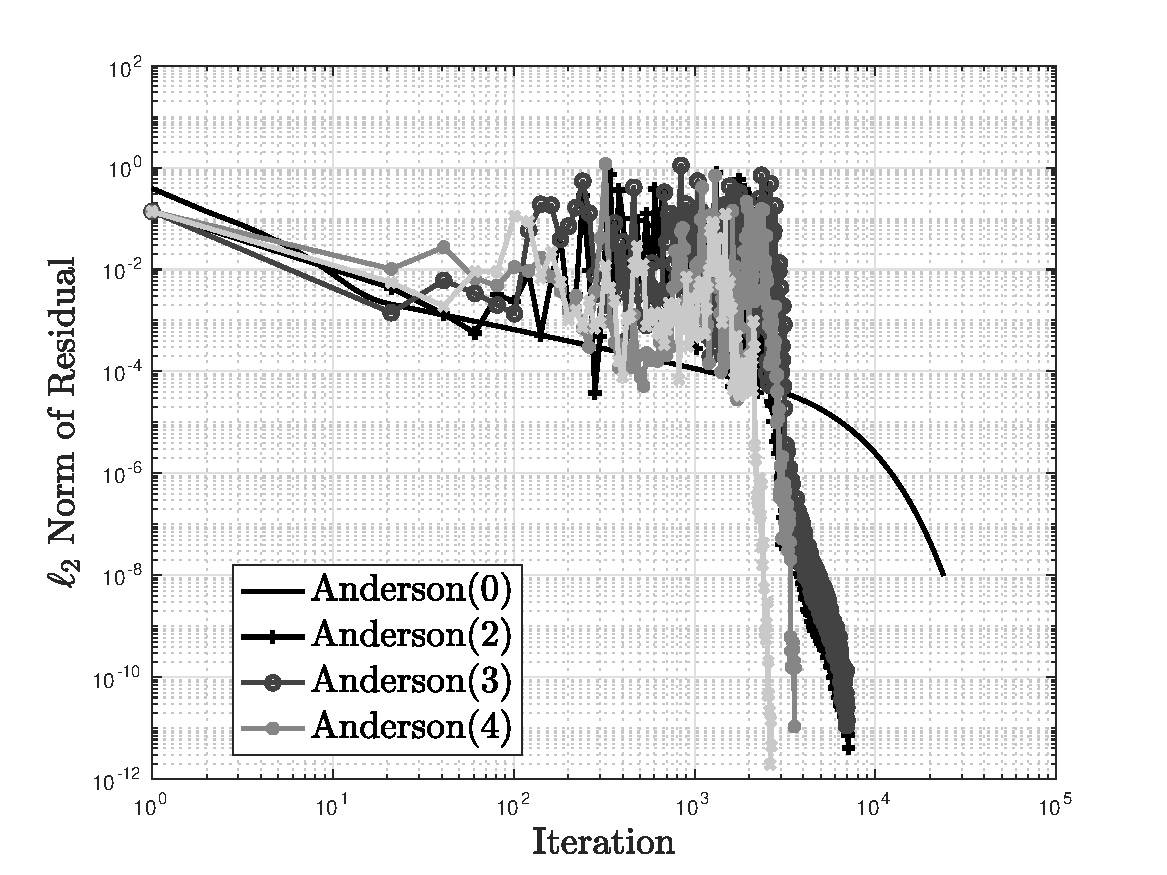
\includegraphics[width=.73\linewidth]{Figures/AndersonAcceleration/SoodProb68_FPI1}
\end{subfigure}
\caption{Anderson Acceleration Convergence for Sood Criticality Problem 68 ($\beta_{n} = 1$), No Initial Fixed-Point Iterations}
\label{fig:AASoodProb68}
\end{figure}

\begin{figure}[!htbp]
\centering
\begin{subfigure}{\textwidth}
  \centering
  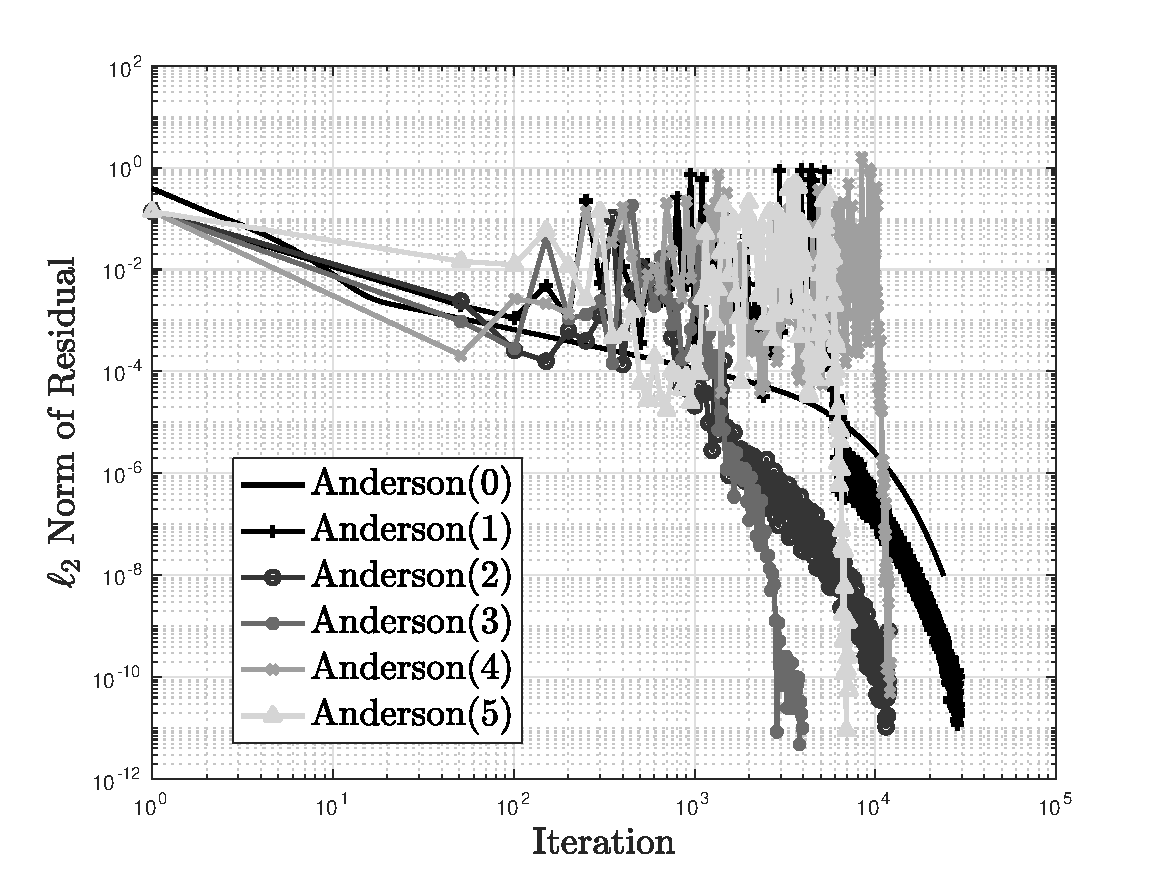
\includegraphics[width=.73\linewidth]{Figures/AndersonAcceleration/SoodProb68_FPI1_HalfBeta}
\end{subfigure}
\caption{Anderson Acceleration Convergence for Sood Criticality Problem 68 ($\beta_{n} = 0.5$), No Initial Fixed-Point Iterations}
\label{fig:AASoodProb68HalfBeta}
\end{figure}

\clearpage

\subsection{Uranium-Heavy Water Critical Slab (Sood Criticality Benchmark Problem 73)}

In this section we examine another uranium-heavy water critical slab problem that is slow to converge when using the Rayleigh Quotient Fixed Point method. Similar to Sood Criticality Benchmark Problem 68, Sood Criticality Benchmark Problem 73 has large amounts of scattering and a large critical width. This problem also contains anisotropic scattering where some of these cross sections are negative. Table~\ref{table:D2O-Sood73} lists the two-group cross sections and Table~\ref{table:Sood73Ref} lists the critical width of the slab and the reference alpha-eigenvalue. The problem was modeled using one hundred spatial cells, step differencing, and S$_{16}$ discrete ordinates angular quadrature.

The number of iterations required to converge the eigenvalue/eigenvector is shown in Table~\ref{table:Sood73AA}. Zero, five, ten, 20, 50, and 100 preliminary fixed-point iteration variants were studied with relaxation factor $\beta_{n} = 1$. The Rayleigh Quotient Fixed Point (Anderson(0)) required 22749 iterations to converge the eigenvalue/eigenvector to an $\ell_{2}$ residual of $10^{-8}$. As before, the tolerance of the Anderson acceleration calculations was set to $10^{-12}$ to prevent false convergence. Unlike Sood Criticality Benchmark Problem 68, it was found that all Anderson acceleration variants converged to the correct eigenvalue. As the number of residual vectors increased, the number of iterations decreased except in the case of five residual vectors. For this number of residual vectors, it was found that the linear system was poorly conditioned.

Increasing the number of initial fixed-point iterations before acceleration only reduces the number of total iterations in some cases. As the number of initial fixed-point iterations increases, it was seen that the number of iterations either remained the same or increased (Table~\ref{table:Sood73AA}). By allowing for more initial iterations, it is possible that the vector iterates ended up much further from the fixed point. If instead the acceleration were turned on sooner, the iterates would instead end up in the region of convergence much sooner.

Figure~\ref{fig:AASoodProb73} shows the convergence behavior of the different Anderson acceleration variants ($\beta_{n} = 1$, zero initial fixed-point iterations) and the Rayleigh Quotient Fixed Point method. The Anderson acceleration variants oscillate substantially until converging to the fixed point. While Anderson(1) only reduced the number of iterations required by a factor of 20\%, Anderson(3) and Anderson(4) reduced iteration number by up to factor of 10. Using relaxation parameter $\beta_{n} = 0.5$, the number of iterations increased. We see a shift toward the right of the convergence behavior in Figure~\ref{fig:AASoodProb73Half}. For this particular problem, the relaxation parameter is not necessary since all Anderson acceleration variants converge onto the right fixed point.

For this particular problem, Anderson acceleration provided substantial reductions in iterations. However, for certain combinations of residual vector number, relaxation parameters, and initial fixed-point iterations, it was found that the acceleration method would not perform as well. Similar to the previous problem, using three or four residual vectors with five or ten initial fixed-point iterations was found to give the best results. This problem, however, shows that the various parameters of Anderson acceleration require optimization.

\begin{table}[!htbp]
	\caption{Two-Group U-D$_{2}$O Problem Cross Sections (cm$^{-1}$)}
	\label{table:D2O-Sood73}
	\begin{subtable}[!htbp]{1.0\textwidth}
		\centering\ra{1.3}
		\begin{tabular}{@{}cccccc@{}}\toprule
			$g$ & $\sigma_{g} $ & $\nu_{g}$ & $\sigma_{fg}$ & $\chi_{g}$ & $v_{g}$ [cm/s] \\ 
        			\midrule
			1 & 0.33588  & 2.50 & 0.002817 & 1.0 & 2.0 \\
			2 & 0.54628  & 2.50 & 0.097 & 0.0 & 1.0 \\
			\bottomrule
		\end{tabular}
	\caption{U-D$_{2}$O(73) Cross Sections}
	\end{subtable}%
	\vspace{0.25cm}
	\begin{subtable}[!htbp]{1.0\textwidth}
	\centering\ra{1.3}
	\begin{tabular}{@{}ccc@{}}\toprule
	$g' \rightarrow g$ & 1 & 2 \\ 
        \midrule
	1 & 0.31980 & 0.004555   \\
	2 & 0.0 & 0.42410  \\
	\bottomrule
	\end{tabular}
	\caption{U-D$_{2}$O(73) Scattering Block-$\sigma_{s0}$}
	\end{subtable}
		\begin{subtable}[!htbp]{1.0\textwidth}
	\centering\ra{1.3}
	\begin{tabular}{@{}ccc@{}}\toprule
	$g' \rightarrow g$ & 1 & 2 \\ 
        \midrule
	1 & 0.06694 & -0.0003972 \\
	2 & 0.0 & 0.05439  \\
	\bottomrule
	\end{tabular}
	\caption{U-D$_{2}$O(73) Scattering Block-$\sigma_{s1}$}
	\end{subtable}
\end{table}

\begin{table}[!htbp]
\caption{Sood Criticality Problem 73 Critical Width and Reference Alpha-Eigenvalue \cite{sood2003analytical}}
	\label{table:Sood73Ref}
	\begin{subtable}[h]{1.0\textwidth}
	\centering\ra{1.3}
	\begin{tabular}{@{}ccc@{}}\toprule
	Cross Section Set & r$_{c}$ [cm] & Reference $\alpha$ [s$^{-1}$] \\
	\midrule
	U-D$_{2}$O(73) & 1000.506133 & $-1.221913 \times 10^{-5}$ \\
	\bottomrule
	\multicolumn{3}{l}{$M = 100$, $L = 16$, Tolerance = $10^{-12}$} \\
	\end{tabular}
	\end{subtable}%
\end{table}

\begin{table}[!htbp]
\caption{Anderson Acceleration for Sood Criticality Problem 73 ($\beta_{n} = 1, M = 100, L = 16$)}
	\label{table:Sood73AA}
	\begin{subtable}[h]{1.0\textwidth}
	\centering\ra{1.3}
	\begin{tabular}{@{}ccc@{}}\toprule
	Anderson($m_{n}$) & Calculated $\alpha$ [s$^{-1}$] & Iterations \\
	\midrule
	Anderson(0) & $-1.221913 \times 10^{-5}$ & 22,749 \\
	Anderson(1) & $-1.221913 \times 10^{-5}$ & 17,620 \\
	Anderson(2) & $-1.221913 \times 10^{-5}$ & 4,814  \\
	Anderson(3) & $-1.221913 \times 10^{-5}$ & 2,777  \\
	Anderson(4) & $-1.221913 \times 10^{-5}$ & 1,854  \\
	Anderson(5) & $-1.221913 \times 10^{-5}$ & 6,008  \\
	\bottomrule
	Initial Fixed-Point Iterations = 0
	\end{tabular}
	\end{subtable}%
	\vspace{0.25cm}
	\begin{subtable}[h]{1.0\textwidth}
	\centering\ra{1.3}
	\begin{tabular}{@{}ccc@{}}\toprule
	Anderson($m_{n}$) & Calculated $\alpha$ [s$^{-1}$] & Iterations \\
	\midrule
	Anderson(1) & $-1.221913 \times 10^{-5}$ & 17,775 \\
	Anderson(2) & $-1.221913 \times 10^{-5}$ & 9,204 \\
	Anderson(3) & $-1.221913 \times 10^{-5}$ & 2,583 \\
	Anderson(4) & $-1.221913 \times 10^{-5}$ & 1,407 \\
	Anderson(5) & $-1.221913 \times 10^{-5}$ & 6,172 \\
	\bottomrule
	Initial Fixed-Point Iterations = 5
	\end{tabular}
	\end{subtable}%
	\vspace{0.25cm}
	\begin{subtable}[h]{1.0\textwidth}
	\centering\ra{1.3}
	\begin{tabular}{@{}ccc@{}}\toprule
	Anderson($m_{n}$) & Calculated $\alpha$ [s$^{-1}$] & Iterations \\
	\midrule
	Anderson(1) & $-1.221913 \times 10^{-5}$ & 12,186 \\
	Anderson(2) & $-1.221913 \times 10^{-5}$ & 11,382 \\
	Anderson(3) & $-1.221913 \times 10^{-5}$ & 4,809 \\
	Anderson(4) & $-1.221913 \times 10^{-5}$ & 2,626 \\
	Anderson(5) & $-1.221913 \times 10^{-5}$ & 3,603 \\
	\bottomrule
	Initial Fixed-Point Iterations = 10
	\end{tabular}
	\end{subtable}
\end{table}

\begin{table}[!htbp]\ContinuedFloat
	\begin{subtable}[h]{1.0\textwidth}
	\centering\ra{1.3}
	\begin{tabular}{@{}ccc@{}}\toprule
	Anderson($m_{n}$) & Calculated $\alpha$ [s$^{-1}$] & Iterations \\
	\midrule
	Anderson(1) & $-1.221913 \times 10^{-5}$ & 12,241 \\
	Anderson(2) & $-1.221913 \times 10^{-5}$ & 3,604  \\
	Anderson(3) & $-1.221913 \times 10^{-5}$ & 6,713  \\
	Anderson(4) & $-1.221913 \times 10^{-5}$ & 5,430  \\
	Anderson(5) & $-1.221913 \times 10^{-5}$ & 2,925  \\
	\bottomrule
	Initial Fixed-Point Iterations = 20
	\end{tabular}
	\end{subtable}%
	\vspace{0.25cm}
	\begin{subtable}[h]{1.0\textwidth}
	\centering\ra{1.3}
	\begin{tabular}{@{}ccc@{}}\toprule
	Anderson($m_{n}$) & Calculated $\alpha$ [s$^{-1}$] & Iterations \\
	\midrule
	Anderson(1) & $-1.221913 \times 10^{-5}$ & 17,166 \\
	Anderson(2) & $-1.221913 \times 10^{-5}$ & 7,363 \\
	Anderson(3) & $-1.221913 \times 10^{-5}$ & 4,205 \\
	Anderson(4) & $-1.221913 \times 10^{-5}$ & 1,729 \\
	Anderson(5) & $-1.221913 \times 10^{-5}$ & 2,253 \\
	\bottomrule
	Initial Fixed-Point Iterations = 50
	\end{tabular}
	\end{subtable}%
	\vspace{0.25cm}
	\begin{subtable}[h]{1.0\textwidth}
	\centering\ra{1.3}
	\begin{tabular}{@{}ccc@{}}\toprule
	Anderson($m_{n}$) & Calculated $\alpha$ [s$^{-1}$] & Iterations \\
	\midrule
	Anderson(1) & $-1.221913 \times 10^{-5}$ & 17,313 \\
	Anderson(2) & $-1.221913 \times 10^{-5}$ & 14,811 \\
	Anderson(3) & $-1.221913 \times 10^{-5}$ & 10,654 \\
	Anderson(4) & $-1.221913 \times 10^{-5}$ & 3,923 \\
	Anderson(5) & $-1.221913 \times 10^{-5}$ & 3,657 \\
	\bottomrule
	Initial Fixed-Point Iterations = 100
	\end{tabular}
	\end{subtable}
\end{table}

\begin{figure}[!htbp]
\centering
\begin{subfigure}{\textwidth}
  \centering
  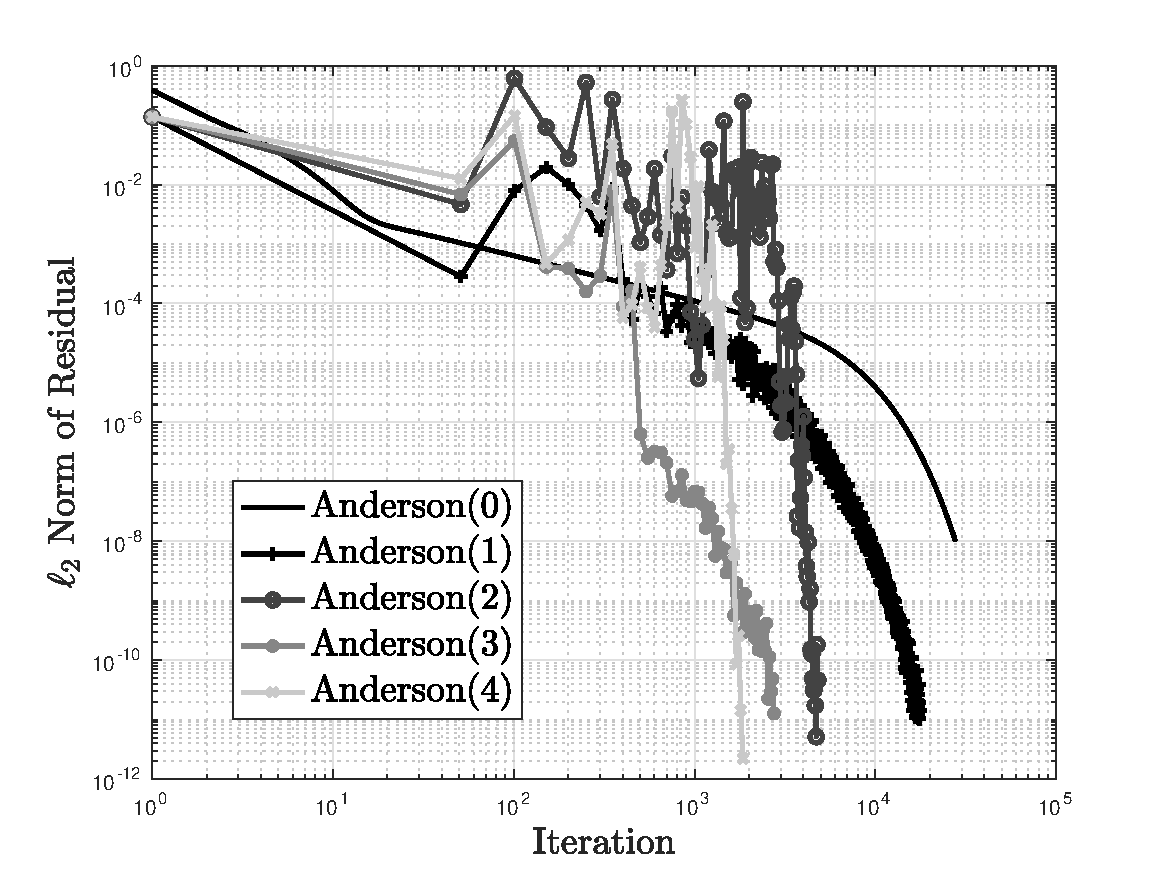
\includegraphics[width=.73\linewidth]{Figures/AndersonAcceleration/SoodProb73}
\end{subfigure}
\caption{Anderson Acceleration Convergence for Sood Criticality Problem 73 ($\beta_{n} = 1$), No Initial Fixed-Point Iterations}
\label{fig:AASoodProb73}
\end{figure}

\begin{figure}[!htbp]
\centering
\begin{subfigure}{\textwidth}
  \centering
  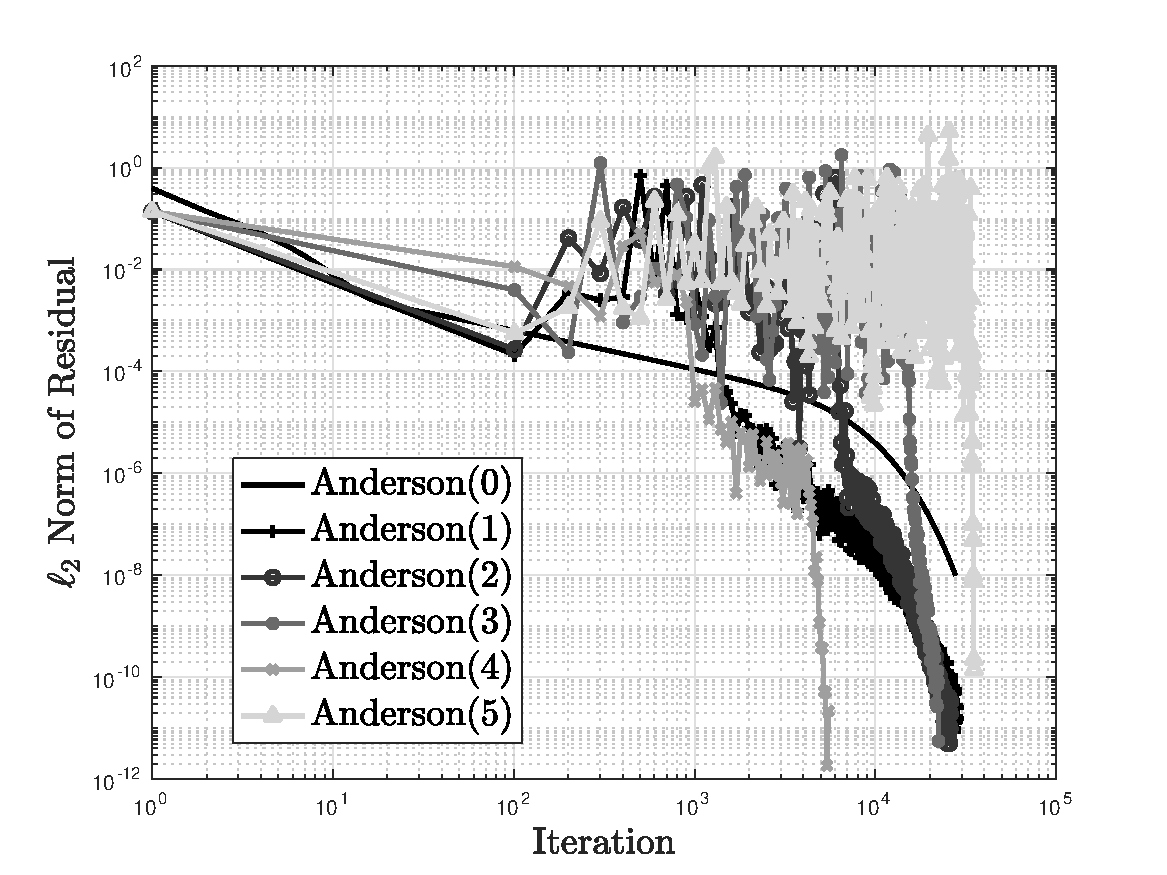
\includegraphics[width=.73\linewidth]{Figures/AndersonAcceleration/SoodProb73_FPI1_HalfBeta}
\end{subfigure}
\caption{Anderson Acceleration Convergence for Sood Criticality Problem 73 ($\beta_{n} = 0.5$), No Initial Fixed-Point Iterations}
\label{fig:AASoodProb73Half}
\end{figure}

\clearpage

\section{Conclusion}

Anderson acceleration was applied to the Rayleigh Quotient Fixed Point method for alpha-eigenvalue problems. Anderson acceleration and its constrained and unconstrained formulations were presented. The unconstrained formulation of Anderson acceleration was implemented in MATLAB and applied to the RQFP method. Two slowly converging one-dimensional slab geometry problems were considered and the number of iterations compared for various variants of the acceleration scheme. The effects of different numbers of residual vectors, relaxation parameters, and initial fixed-point iterations before acceleration were considered and their effects on the ability of the method to converge to the fundamental eigenvector and eigenvalue were discussed. It was found that while larger numbers of residual vectors produced faster convergence, the memory required quickly increased. Instead it was found that using a combination of initial fixed-point iterations and a lesser number of residual vectors produced substantial speedups. In particular, the initial fixed-point iterations were found to help the method to converge to the correct eigenpair by allowing the vector iterate to enter the region of convergence for the fixed point. Using a relaxation parameter also improves the ability of the method to converge by reducing step lengths when the vector iterate is not near the fixed-point solution. Despite the fact Anderson acceleration required tighter tolerance to prevent false convergence, the reduction in iterations required for convergence is substantial and should be considered for slowly converging problems. 
\chapter{Conclusion}
\label{ch:Conc}

This dissertation described the derivation and mathematical foundation of the Rayleigh Quotient Fixed Point method and its use to determine the alpha- and $k$-effective eigenvalue criticality problems in neutron transport. The Rayleigh Quotient Fixed Point method is a non-linear fixed point method that uses the proven primitivity property of the discretized neutron transport eigenvalue equations to find the positive angular flux eigenvector solution and corresponding eigenvalue. This dissertation discusses the application of the Rayleigh Quotient Fixed Point method to infinite media, one-dimensional slabs and sphere, as well as realistic two- and three-dimensional reactor models using the neutral particle transport code ARDRA \cite{hanebutte_ardra_1999}.

For alpha-eigenvalue problems, previous methods were limited to transport-based matrix method or criticality search iterative schemes. For transport-based matrix methods, the discretized matrices of the alpha-eigenvalue were formed and traditional eigenvalue solution methods were applied. These methods become increasingly expensive in memory and computational effort as problems increase in complexity. For criticality search iterative schemes, the alpha-eigenvalue is determined by relating the eigenvalue to another eigenvalue problem, the $k$-effective eigenvalue. These methods require multiple $k$-effective eigenvalue calculations to converge the alpha-eigenvalue, increasing the number of transport sweeps required to converge the alpha-eigenvalue. A substantial amount of iterations are spent determining an eigenvalue not of interest to the problem. Furthermore, there remain open questions as to how converged the proxy eigenvalue calculation must be to allow for convergence of the alpha-eigenvalue problem. These methods also historically have been applied to supercritical nuclear systems, being of limited use for subcritical problems that are become more of interest in the recent years. The Rayleigh Quotient Fixed Point for alpha-eigenvalue problems is an iterative method that uses an eigenvalue update that is optimal in the least squares sense. The Rayleigh Quotient Fixed Point method directly updates the alpha-eigenvalue, not requiring knowledge of any other eigenvalue, substantially reducing the number of iterations required for convergence. Additionally, it is able to solve subcritical. critical, and supercritical systems, providing a more general solution method to alpha-eigenvalue problems.

For $k$-effective problems, the traditional workhorse method, the power method, traditionally used a fission source update for the eigenvalue at each iteration. By using the Rayleigh Quotient Fixed Point method, the $k$-effective eigenvalue problem can be viewed as a non-linear fixed point method where an optimal update for the eigenvalue can be derived. In certain circumstances, this provides a reduction in transport sweeps necessary to converge the eigenvalue and eigenvector of interest.

Throughout the derivation of the Rayleigh Quotient Fixed Point method, the primitivity property of the discretized eigenvalue equations was used to guarantee the existence of a unique positive eigenvector corresponding to the spectral radius as stated in the Perron-Froebenius theory for primitive matrices. It was shown that for a one-dimensional slab geometry eigenvalue problem discretized with diamond differencing in space, discrete ordinates angular quadrature, and the multigroup-in-energy approximation, the discretized linear system is a primitive system with index of primitivity of two. This result is similar to that of Mokhtar-Kharroubi where it was found that the continuous neutron transport equation eigenvalue problem was \textit{positivity-improving} or primitive with index of primitivity of two \cite{mokhtar1997mathematical}.The existence of a unique eigenvector and a way to relate it to either the alpha- or $k$-effective eigenvalue provided a powerful tool to derive a fixed point method capable of determining the eigenvalue and the physical, positive angular flux eigenvector.

The Rayleigh Quotient Fixed Point method for alpha- and $k$-effective eigenvalues accurately determined the alpha- and $k$-effective eigenvalues of various analytic, infinite-medium problems by Betzler \cite{Betzler2014Alpha}. It was also demonstrated the failure of the eigenvalue problem when the conditions of irreducibility and primitivity failed to exist and how these problems were unphysical in most cases. Next, the method was validated for one-dimensional slabs and spheres and compared to the Green's Function Method of Kornreich and Parsons \cite{kornreich_timeeigenvalue_2005}. The number of transport sweeps required by the Rayleigh Quotient Fixed Point method was compared to the standard solvers, showing that the RQFP method provided major reductions in the number of iterations required for convergence and the ability to converge problems where other methods failed. Next, realistic two-dimensional cylindrical problems and two- and three-dimensional fuel assembly benchmark problems were analyzed to show the general applicability of the RQFP method even when some of the assumptions made in deriving the method did not apply. Transport sweep comparisons were used to show the improvement the RQFP method provides over traditional eigenvalue solvers for both alpha- and $k$-effective eigenvalue problems. For realistic reactor problems with large amounts of materials, energies, and other heterogeneities, the RQFP method outperformed the standard eigensolvers.



\printbibliography

\appendix
\chapter[Discretization of the Alpha-Eigenvalue Problem For Slab Geometry][Discretized Slab Alpha-Eigenvalue Problem]{Discretization of the Alpha-Eigenvalue Problem For Slab Geometry}

\label{Discrete1D}

In Appendix~\ref{Discrete1D}, we describe the discretization of the alpha-eigenvalue problem for one-dimensional slab geometry using a matrix formalism similar to that of three-dimensional Cartesian geometry. In one dimension, the discretization of the continuous eigenvalue equation is substantially simpler and may be helpful to reader to study this case before analyzing the three-dimensional problem.

We begin with the alpha-eigenvalue transport equation in one-dimensional slab geometry with isotropic scattering. The spatial domain is the interval $[a,b]$ in $x$, $\mu$ is the angle cosine in $[-1,1]$, the energy variable is $E \in [0, \infty)$, and the equations for the angular flux $\psi(x, \mu, E)$ are given by
\begin{multline}
\bigg [ \mu \frac{\partial}{\partial x} + \frac{\alpha}{v(E)} + \sigma(x,E) \bigg ] \psi(x,\mu,E) \\ = \frac{\chi(E)}{2} \int_{0}^{\infty} \diff E' \nu(E') \sigma_{f}(x,E') \int_{-1}^{1} \diff \mu' \psi(x,\mu',E) \\ + \frac{1}{2} \int_{0}^{\infty} \diff E' \sigma_{s}(x, E' \rightarrow E) \int_{-1}^{1} \diff \mu' \psi(x,\mu',E).
\label{eq:1DAlpha}
\end{multline}
We assume vacuum Dirichlet conditions
\begin{align}
	\psi(a, \mu, E) &=0, \quad 0 < \mu \leq 1, \\
        \psi(b, \mu, E) &=0, \quad -1 \leq \mu < 0.
\end{align}
The discretization of Eqn~\ref{eq:1DAlpha} is done using diamond differencing in space, multigroup in energy, and discrete ordinates collocation in angle.

\section{Discretization of the One-Dimensional Slab Geometry Problem}

We begin by discretizing Eq.~\ref{eq:1DAlpha} in energy using the \textit{multigroup} approximation. We restrict the energy $E$ to a finite interval and partition the interval into groups:
\begin{equation}
	E_{max} = E_{0} > E_{1} > \dots > E_{G} = E_{min}.
\end{equation}
The eigenvalue equation is then averaged over each group $E_{g} < E < E_{g-1}$ and the cross sections are approximated by a flux-weighted average over each energy group. In the spatial dimension, we introduce a spatial grid
\begin{equation}
	a \equiv x_{0} < \dots < x_{i+1} < x_{i} < \dots < x_{M} \equiv b,
\end{equation}
and let 
\begin{equation}
\Delta x_{i} = x_{i} - x_{i-1}.
\end{equation} 
We refer to the $x_{i}$ as nodes and function values at the nodes are called nodal values. We assume that $\sigma_{g}$ and $\sigma_{s,g,g'}$, the total and scattering cross sections for energy group $g$, are constant on the zone $x_{i-1} < x < x_{i}$ and denote these values by $\sigma_{g,i}$ and $\sigma_{s,g,g',i}$. We use a discrete ordinates collocation of Eq.~\ref{eq:1DAlpha} at an even number of Gauss points $\mu_{\ell}$ with
\begin{equation}
	-1 < \mu_{1} < \dots < \mu_{L/2} < 0 < \mu_{L/2+1} < \dots < \mu_{L} < 1, \mu_{L+1-\ell} = - \mu_{\ell}.
\end{equation}
The integrals in angle in Eq.~\ref{eq:1DAlpha} are then approximated by
\begin{equation}
	\frac{1}{2} \int_{-1}^{1} \diff \mu \, \psi_{g}(x, \mu) \approx \sum_{\ell=1}^{L} w_{\ell} \psi_{g}(x, \mu_{\ell}).
\end{equation}
Using diamond differencing in the spatial dimension \cite{lewis_computational_1984}, we obtain the fully discretized set of equations for the eigenvalue problems
\begin{multline}
	\mu_{\ell} \frac{ \psi_{g,\ell,i} - \psi_{g, \ell, i-1}}{\Delta x_{i}} + \frac{\alpha}{v_{g}} \frac{\psi_{g,\ell,i} + \psi_{g, \ell, i-1}}{2} + \sigma_{g,i} \frac{\psi_{g,\ell,i} + \psi_{g, \ell, i-1}}{2} \\ = \frac{\chi_{g}}{2} \sum_{g'=1}^{G} \frac{\nu_{g}\sigma_{f,g',i}}{2} \sum_{\ell' = 1}^{L} w_{\ell'} \bigg ( \frac{\psi_{g',\ell',i} + \psi_{g',\ell',i-1} }{2} \bigg ) + \sum_{g'=1}^{G} \frac{\sigma_{s,g,g',i}}{2} \sum_{\ell' = 1}^{L} w_{\ell'} \bigg ( \frac{\psi_{g',\ell',i} + \psi_{g',\ell',i-1} }{2} \bigg ),
\label{eq:AlphaSlab}
\end{multline}
for $g = 1, \dots, G$, $i = 1, \dots, M$, and $\ell = 1, \dots, L$. The discretized boundary conditions are given by
\begin{align}
\psi_{g,\ell,M} &= 0 \text{ for } \ell = 1, \dots, L/2,  \\
\psi_{g,\ell,0} &= 0 \text{ for } \ell = L/2+1, \dots, L.
\end{align}
Using cell-centered flux values, it follows that Eq.~\ref{eq:AlphaSlab} is a system of $GL(M+1)$ equations for $GL(M+1)$ unknowns. 

%\subsection{The Diamond Difference Operator Matrix Form}

To write Eq.~\ref{eq:AlphaSlab} in matrix form, we define the angular flux vector for a single energy group $g$ as
\begin{equation}
\Psi_{g} \equiv 
\begin{pmatrix}
\Psi_{g,1} \\
\vdots \\
\Psi_{g,L}
\end{pmatrix} \in \mathbb{R}^{L(M+1)} \quad \text{ with } \quad
\Psi_{g, \ell} \equiv 
\begin{pmatrix}
\psi_{g,\ell,0} \\
\vdots \\
\psi_{g,L,M}
\end{pmatrix} \in \mathbb{R}^{M+1}.
\end{equation}
To write the matrix form of the diamond difference discretized operator $\mu_{\ell} \partial/\partial x + 1/v_{g} + \sigma_{g}$, we define the block diagonal matrix
\begin{equation}
\bar{S} \equiv \text{diag}(S_{1}, \dots, S_{L}) \in \mathbb{R}^{LM \times L(M+1)}
\end{equation}
with
\begin{equation}
S_{\ell} = S = \frac{1}{2}
\setlength\arraycolsep{2pt}
\begin{pmatrix}
1 & 1 & & \\
& \ddots & \ddots & \\
& & 1 & 1
\end{pmatrix} \in \mathbb{R}^{M \times (M+1)},
\end{equation}
for all $\ell$. The matrix $S$ interpolates nodal vectors into zone-centered vectors by averaging the nodal values. Now we define the total cross section and inverse velocity matrices for energy group $g$ as
\begin{equation}
	\Sigma_{g}  \equiv \text{diag}(\sigma_{g,1},\dots,\sigma_{g,M}) \in \mathbb{R}^{M \times M},
\end{equation}
\begin{equation}
	V^{-1}_{g}  \equiv \text{diag}(1/v_{g,1},\dots,1/v_{g,M}) \in \mathbb{R}^{M \times M}.
\end{equation}
We define the following matrices to describe the discretized derivative term
\begin{equation}
	\Delta x \equiv \text{diag}(\Delta x_{1}, \dots, \Delta x_{M}) \in \mathbb{R}^{M \times M}
\end{equation}
and
\begin{equation}
D \equiv
\setlength\arraycolsep{2pt}
\begin{pmatrix}
-1 & 1 & & \\
& \ddots & \ddots & \\
& & -1 & 1
\end{pmatrix} \in \mathbb{R}^{M \times (M+1)}.
\end{equation}
Boundary values are isolated by defining the row vector
\begin{equation}
	B_{\ell} \equiv \begin{cases}
				e_{M}^{T} \quad \text{ if } \ell \leq L/2, \\
				e_{0}^{T}  \quad \text{ if } \ell > L/2,
                              \end{cases} \in \mathbb{R}^{M+1},
\end{equation}
where the indices on the standard basis vectors $e_{\ell}$ are from 0 to $M$. Finally, we define the matrices $Z$ and $Z_{b}$ as
\begin{equation}
	Z \equiv \begin{pmatrix}
			I_{M} \\
			0
		     \end{pmatrix} \in \mathbb{R}^{(M+1) \times M} \quad \text{ and } \quad
	Z_{b} \equiv  e_{M}.
\end{equation}
We can now define the matrix form of the diamond difference representation of  $\mu_{\ell} \partial/\partial x + \alpha/v_{g} + \sigma_{g}$ as 
\begin{equation}
	H_{g} + \alpha V^{-1}_{g} \equiv \text{diag}(H_{g,1}, \dots, H_{g,L}) + \alpha \text{ diag}(V^{-1}_{g,1}, \dots, V^{-1}_{g,L}) \in \mathbf{R}^{L(M+1)},
\end{equation}
where
\begin{equation}
	H_{g,\ell} + \alpha V^{-1}_{g,\ell} \equiv Z(\mu_{\ell}\Delta x^{-1}D + \Sigma_{g}S_{\ell}) + Z_{b}B_{\ell} + \alpha ZV_{g}^{-1}S_{\ell}.
\end{equation}
It can be shown that $H_{g} + \alpha V^{-1}_{g}$ is nonsingular for the diamond difference method if $\alpha$ is not too negative.

We now define discretized representations of angular flux moment operators. The matrices operate on zone-centered vectors and are in $\mathbb{R}^{M \times LM}$. We define the matrix
\begin{equation}
	L_{n} \equiv (l_{n}W) \otimes I_{M},
\end{equation}
where $l_{n} \equiv (P_{n}(\mu_{1}), P_{n}(\mu_{2}), \dots, P_{n}(\mu_{L}))$ are the Legendre polynomials and the quadrature weights are given by $W \equiv \text{diag}(w_{1}, \dots, w_{L})$.
If the vector $\Psi_{g}$ approximates $\psi_{g}(x, \mu)$, then $L_{n}\Psi_{g}$ approximates taking the n$^{th}$ moment of the angular flux $\phi_{g,n}(x)$. We also define the matrix
\begin{equation}
	L_{n}^{+} \equiv (2n+1)l_{n}^{T} \otimes I_{M} \in \mathbb{R}^{LM \times M}.
\end{equation}
If a vector $\Phi$ approximates $\phi(x)$, then $L_{n}^{+}\Psi$ will approximate $P_{n}(\mu)\phi(x)$. We define the grouped matrices for $N_{s}$ moments as
\begin{equation}
L^{N} = \begin{pmatrix}
		L_{0} \\
		\vdots \\
		L_{N}
	     \end{pmatrix} \quad \text{ and } \quad
L^{N,+} = (L_{0}^{+}, \dots, L_{N}^{+}).
\end{equation}
We can define the scattering and fission matrices as
\begin{equation}
	\Sigma_{s,g,g',n} \equiv \text{diag}(\sigma_{s,g,g',n,1}, \dots, \sigma_{s,g,g',n,M}) \in \mathbb{R}^{M \times M}
\end{equation}
and
\begin{equation}
	\Sigma_{f,g,g',n} \equiv \text{diag}(\chi_{g}\nu\sigma_{f,g',n,1}, \dots, \chi_{g}\nu\sigma_{f,g',n,M}) \in \mathbb{R}^{M \times M}.
\end{equation}
We now define matrices that inject zone-centered vectors into nodal vector space and vice versa. We define the matrices
\begin{equation}
\bar{\Sigma}_{g} \equiv I_{L} \otimes \Sigma_{g} \in \mathbb{R}^{LM \times LM},
\end{equation}
\begin{equation}
\bar{V^{-1}}_{g} \equiv I_{L} \otimes V^{-1}_{g} \in \mathbb{R}^{LM \times LM},
\end{equation}
\begin{equation}
	\bar{Z} = I_{L} \otimes Z \in \mathbb{R}^{L(M+1) \times LM},
\end{equation}
\begin{equation}
	\bar{Z}_{B} = I_{L} \otimes Z_{b} \in \mathbb{R}^{L(M+1) \times L},
\end{equation}
\begin{equation}
	B = \text{diag}(B_{1}, \dots, B_{L}) \in \mathbb{R}^{L \times L(M+1)},
\end{equation}
and
\begin{equation}
	C = \text{diag}(\mu_{1}\Delta x^{-1}D, \dots, \mu_{L} \Delta x^{-1}D) \in \mathbb{R}^{LM \times L(M+1)}.
\end{equation}
Using the above matrices, we can write the matrix $H_{g} + V^{-1}_{g}$ as
\begin{multline}
H_{g} + V^{-1}_{g} \equiv \text{diag}(H_{g,1}, \dots, H_{g,L}) + \text{diag}(V^{-1}_{g,1}, \dots, V^{-1}_{g,L}) \\ = \bar{Z}(C + \bar{\Sigma}_{g}\bar{S}) + \bar{Z}_{B}B + \bar{Z}\bar{V}^{-1}\bar{S}.
\end{multline}
The discretized multigroup eigenvalue equations can then be written in the matrix form as
\begin{equation}
	H_{g} \Psi_{g} + \alpha V^{-1}_{g}\Psi_{g} = \bar{Z} \sum_{g'=1}^{G} \sum_{n=0}^{N_{s}} L_{n}^{+}\Sigma_{s,g,g',n}L_{n}\bar{S}\Psi_{g'}  +  \bar{Z} \sum_{g'=1}^{G} \sum_{n=0}^{N_{s}} L_{n}^{+}\Sigma_{f,g,g',n}L_{n}\bar{S}\Psi_{g'}, 
	\label{eq:AlphaMGg}
\end{equation}
Finally, we can write the multigroup discretized eigenvalue equations if we define the matrices
\begin{equation}
	\mathbf{\Psi} \equiv \begin{pmatrix}
					\Psi_{1} \\
					\Psi_{2} \\
					\vdots \\
					\Psi_{G}
				       \end{pmatrix}, \quad
	\mathbf{\Sigma_{s}} \equiv \begin{pmatrix}
					\Sigma_{s, 11}^{N_{s}} & \dots & \Sigma_{s,1G}^{N_{s}} \\
					\vdots & \ddots & \vdots \\
					\Sigma_{s, G1}^{N_{s}} & \dots & \Sigma_{s,GG}^{N_{s}}
					\end{pmatrix}, \quad 
	\mathbf{\Sigma_{f}} \equiv \begin{pmatrix}
					\Sigma_{f, 11}^{N_{s}} & \dots & \Sigma_{f,1G}^{N_{s}} \\
					\vdots & \ddots & \vdots \\
					\Sigma_{f, G1}^{N_{s}} & \dots & \Sigma_{f,GG}^{N_{s}}
					\end{pmatrix},
\end{equation}
where 
\begin{equation}
\Sigma_{s,gg'}^{N_{s}} \equiv \text{diag}(\Sigma_{s,g,g',0}, \dots, \Sigma_{s,g,g',N_{s}})
\end{equation}
and
\begin{equation}
\Sigma_{f,gg'}^{N_{s}} \equiv \text{diag}(\Sigma_{f,g,g',0}, \dots, \Sigma_{f,g,g',N_{s}}).
\end{equation}
Defining the following matrices 
\begin{equation}
\mathbf{S} \equiv I_{G} \otimes \bar{S},
\end{equation} 
\begin{equation}
\mathbf{Z} \equiv I_{G} \otimes \bar{Z},
\end{equation}
\begin{equation}
\mathbf{H} + \mathbf{V}^{-1} \equiv \text{diag}(H_{1} + V^{-1}_{1}, H_{2} + V^{-1}_{2}, \dots, H_{G} + V^{-1}_{G}),
\end{equation}
\begin{equation}
\mathbf{L}^{+} \equiv I_{G} \otimes L^{N_{s},+},
\end{equation}
\begin{equation}
\mathbf{L} \equiv I_{G} \otimes L^{N_{s}},
\end{equation} 
then Eq.~\ref{eq:AlphaMGg} can be written as
\begin{equation}
	\big ( \mathbf{H} + \alpha \mathbf{V}^{-1} \big ) \mathbf{\Psi} = \mathbf{Z} \mathbf{L}^{+}  \big ( \mathbf{\Sigma_{s}} + \mathbf{\Sigma_{f}} \big )\mathbf{L} \mathbf{S} \mathbf{\Psi}.
	\label{AlphaMG}
\end{equation}
Similarly, the discretized $k$-eigenvalue problem can be written as
\begin{equation}
	\mathbf{H}\mathbf{\Psi}  = \mathbf{Z} \mathbf{L}^{+} \bigg ( \mathbf{\Sigma_{s}} + \frac{1}{k} \mathbf{\Sigma_{f}} \bigg ) \mathbf{L} \mathbf{S} \mathbf{\Psi}.
	\label{kMG}
\end{equation}

Equations~\ref{AlphaMG} and \ref{kMG} are eigenvalue equations for the criticality eigenvalue and the node-centered angular flux eigenvector. In the derivation of the Rayleigh Quotient Fixed Point method, an inner product is required. However, the inner product is defined for zone-centered vectors, whereas the unknown angular flux vectors in Eqns.~\ref{AlphaMG} and \ref{kMG} are node-centered. To satisfy this requirement, Eqns.~\ref{AlphaMG} and \ref{kMG} are rewritten using zone-centered angular flux eigenvectors. We denote $\mathbf{\Psi_{z}}$ as the zone-centered unknown and $\mathbf{H_{z}}$ as the zone-centered version of $\mathbf{H}$.
\chapter[Implementation of Anderson Acceleration in MATLAB for the Alpha-Eigenvalue Rayleigh Quotient Fixed Point Method][Anderson Acceleration MATLAB Implementation]{Implementation of Anderson Acceleration in MATLAB for the Alpha-Eigenvalue Rayleigh Quotient Fixed Point Method}

\label{AnderAccMATLAB}

\section{Alpha-Eigenvalue Rayleigh Quotient Fixed Point Method MATLAB Implementation}
\lstinputlisting[numbers=none]{MATLAB/AlphaRQSweep.m}

\section{Anderson Acceleration MATLAB Implementation}
\lstinputlisting[numbers=none]{MATLAB/AnderAccel.m}
% \chapter{More Monticello Candidates}

\end{document}
